%%%%%%%%%%%%%%%%%%%%%%%%%%%%%%%%%%%%%%%%%%%%%%%%%%%%%%%%%%%%%%%%%%%%%%%%%%%%%%%%
%\documentclass[12pt,papel,twoside]{ibtesis}
% \documentclass[12pt]{ibtesis}

% \documentclass[12pt,papel,oneside]{ibtesis}
\documentclass[12pt,papel,twoside,pagebackref]{ibtesis}
% \documentclass[11pt,papel,oneside, singlespace]{ibtesis}

% \documentclass[12pt,papel,preprint,singlespace,oneside]{ibtesis}

%%%%%%%%%%%%%%%%%%%%% Paquetes extra %%%%%%%%%%%%%%%%%%%%%%%%%%%%%%%%%%%%%%%%%%%
% Por conveniencia: aqu\'{\i} puede cargar todos los paquetes y definir los comandos 
% que necesite
\usepackage{ibextra}
\usepackage[utf8]{inputenc}
\usepackage{subcaption}  % Enable figure captions or figure notes
\usepackage{float}
\usepackage{nicefrac}
\usepackage{mathtools}
\usepackage{textcomp}

\usepackage{multirow}
\usepackage{amsfonts}

\usepackage{hyperref}
\usepackage{tablefootnote}

\usepackage{scalerel}
\usepackage{physics}
\usepackage{xcolor}

\usepackage{xparse}
\let\realItem\item % save a copy of the original item
\makeatletter
\NewDocumentCommand\myItem{ o }{%
   \IfNoValueTF{#1}%
      {\realItem}% add an item
      {\realItem[#1]\def\@currentlabel{#1}}% add an item and update label
}
\makeatother

\usepackage{notoccite}

\usepackage{enumitem}    
\setlist[enumerate]{
    before=\let\item\myItem%,       % use \myItem in enumerate
    %label=\textnormal{(\arabic*)}, % format the label
    %widest=(2')                    % set the widest label
}


%%%%%%%%%%%%%%%%%%%%%%%%%%%%%%%%%%%%%%%%%%%%%%%%%%%%%%%%%%%%%%%%%%%%%%%%%%%%%%%%
%%%%%%%%%%%%%%%%%%%%% Información sobre la tesis %%%%%%%%%%%%%%%%%%%%%%%%%%%%%%%
\title{Análisis de las direcciones de arribo de rayos cósmicos de ultra-alta energía en el Observatorio Pierre Auger}
\author{Evelyn~Gabriela~Coronel}
\director{Dra.~Silvia Mollerach}
%\codirector{Dr.~J.~Otro m\'{a}s}b
\carrera{Tesis de Maestría en Ciencias Físicas}
\grado{Maestrando}
\laboratorio{Partículas y Campos -- Centro Atómico Bariloche}
\jurado{ 
	{
		Dr.~Diego~Harari 

		Dra.~Geraldina~Golup  
		
		Dr.~Xavier~Bertou 
		}
 }

\palabrasclave{Rayos Cósmicos, Análisis de datos, Instituto Balseiro}
%\keywords{Cosmic Rays, Data Analysis, Balseiro Institute}
%\neembaeguasu{Mba'e michĩ yvágagui ouva, Mbo'ehaoguasu Balseiro}
% Si queremos poner la fecha manualmente:
% \date{Diciembre de 2099}

%%%%%%%%%%%%%%%%%%%%%%%%%%%%%%%%%%%%%%%%%%%%%%%%%%%%%%%%%%%%%%%%%%%%%%%%%%%%%%%%
%\titlepagefalse % Si no quiere compilar la portada descomente esta linea
%\includeonly{apendices} % Compilar s\'{o}lo estos archivos 
%\graphicspath{{/h}} % Lugar donde encontrar las figuras generales (se puede poner uno en cada cap{\'{\i}}tulo)
%%%%%%%%%%%%%%%%%%%%%%%%%%%%%%%%%%%%%%%%%%%%%%%%%%%%%%%%%%%%%%%%%%%%%%%%%%%%%%%%


%\setcounter{tocdepth}{4}
%\setcounter{secnumdepth}{4}
\begin{document}

\begin{preliminary}

%%% Índices %%%%

\begin{abreviaturas}

\begin{tabular}{l l}
CR: 		& Rayos cósmicos  (\emph{Cosmic Rays}) \\
CMB: 		& Radiación Cósmica de Fondo (\emph{Cosmic Microwave Background})\\
FD: 		& Detector de Fluorescencia (\emph{Fluorescence Detector}) \\
HEAT:		& Telescopios de Auger de Alta Elevación (\emph{High Elevation Auger Telescopes})\\
SD: 		& Detector de Superficie (\emph{Surface Detector})  \\
WCD: 		& Detector de radiación Cherenkov de agua\\
EAS: 		& Lluvia Atmosférica Extendida  (\emph{Extensive Air Shower})    \\
VAOD: 		& Profundidad atmosférica óptica vertical (\emph{Vertical} \\
			& \emph{Atmosferic Optical Depth})\\
CLF:		& \emph{Central Laser Facility}\\
XLF:		& \emph{eXtreme Laser Facility}\\
X$_{max}$: 	& Profundidad atmosférica del máximo de la lluvia \\
LDF: 		& Función de Distribución Lateral (\emph{Lateral Distribution Function}) \\
S(1000): 	& Señal a 1000\,m del núcleo de la lluvia y al nivel del suelo \\
S(1000)$_w$:& Señal de S(1000) corregida por la modulación del clima. \\
CIC: 		& Corte de Intensidad Constante (\emph{Constant Intensity Cut}) \\
S$_{38}$: 	& Señal a 1000\,m del núcleo y al nivel del suelo si el ángulo\\
			& cenital del evento fuera de $38^o$\\
S$_{38,w}$: & Señal S$_{38}$ corregida por la modulación del clima \\
eV: 		& electrón Voltio, $1\,$eV$= 1.602\times 10^{-19}\,$J \\
EeV: 		& $1\,$EeV$=10^{18}\,$eV\\
PMT: 		& Tubo fotomultiplicador (\emph{Photo-Multiplier Tube})\\
VEM: 		& Muón vertical equivalente (\emph{Vertical Equivalent Muon})\\
ICRC: 		& Conferencia Internacional de Rayos Cósmicos \\
			& (\emph{International Cosmic Ray Conference})\\
EW:			& Método East - West\\
Ray:		& Método de Rayleigh\\
msnm:		& Metros Sobre el Nivel del Mar\\
ToT:		& Tiempo por encima del umbral (\emph{Time over Threshold})\\
ToTd		& Tiempo por encima del umbral deconvolucionado (\emph{Time over }\\
			&  \emph{Threshold deconvoluted})\\
MoPS		& Cantidad de pasos positivos (\emph{Multiplicity of Positive Steps})\\
\end{tabular}
                     %Abreviaturas
\end{abreviaturas}

	\tableofcontents                %Indice
	\listoffigures                  %Figuras
	\listoftables                   %Tablas

	\begin{resumen}%
Cuando un rayo cósmico interactúa con una molécula en la parte superior de la atmósfera, se inicia un proceso en el cual se generan otras partículas secundarias. Este proceso es conocido como lluvia atmosférica extendida. Estas lluvias pueden ser detectadas sobre la superficie de la Tierra mediante varios experimentos. Este trabajo utiliza los datos recolectados por los detectores de superficie separados en 1500\,m entre sí del Observatorio Pierre Auger durante los años 2005-2020. 

Se estudian eventos obtenidos mediante distintos algoritmos de adquisición de datos. El \emph{Disparo Estándar} que alcanza eficiencia completa para eventos asociados a rayos cósmicos de energía mayor a $3\,$EeV, y el \emph{Todos los Disparos} llega a detectar, con una eficiencia del 100\%, eventos por encima de $1\,$EeV. El primer disparo contiene eventos registrados desde el año 2005 y el segundo disparo empezó funcionar desde el 2013. 

Las condiciones atmosféricas como la presión (P), la temperatura (T) y la densidad ($\rho \propto \nicefrac{P}{T}$) afectan el desarrollo de la lluvia a través de la atmósfera. Las variaciones de estas condiciones inducen una modulación en la señal producida en los detectores por un rayo cósmico de una dada energía. Mediante un estudio hecho por la Colaboración sobre eventos del Disparo Estándar, se corrigió el efecto de esta modulación en la estimación de la energía de los rayos cósmicos medidos por el Observatorio. En este trabajo extendimos el periodo de tiempo analizado de esta modulación, y se observó que los parámetros obtenidos son comparables con la reconstrucción oficial. También se estudia la modulación en los datos de Todos los Disparos, y se realiza una corrección sobre el mismo conjunto de datos usando los parámetros obtenidos por este trabajo.

Se  estudian las modulaciones en distintas frecuencias mediante el análisis en Rayleigh, y se propone una variable generalizada para hacer un barrido en frecuencias con el método de East-West. Se obtienen resultados de la modulación en ascensión recta para distintos rangos de energía y se comparan con resultados reportados por la Colaboración Pierre Auger.

\end{resumen}


% \begin{nemombyky}%
% Mbyjakua\'ape (\emph{astronomía} karaiñe'\~eme) ojeikuaase mba\textquotesingle e oik\'ova umi mba\textquotesingle e  michĩ yv\'agagui o\'uva (\emph{rayos cósmicos} karaiñe'\~eme) oguah\~evove amo yvatetépe (\emph{atmósfera} karaiñe'\~eme). Ombok\'aramo tuminguaave\textquotesingle \~yty (\emph{conjunto de átomos o molécula}  karaiñe'\~eme ) yvatetépe oĩva, oñepyr\~u ojapo het\~a umi tuminguaave\textquotesingle \~yjokaku\'era (\emph{partículas}  karaiñe'\~eme ) op\'arupi. Ko\textquotesingle a       ha\textquotesingle e  h\'ina peteĩ ama guasu tuminguaave\textquotesingle \~yjoka rehegua ( \emph{lluvia atmosf\'erica extendida} karaiñe'\~eme). Umi ama guasuku\'era tuichaterei ha ikatu eñeña\textquotesingle ã yvy ári op\'arupi. Mend\'osape oĩ peteĩ mba\textquotesingle etuicha h\'erava \emph{Pierre Auger} Mbyjañama\textquotesingle \~eha\~gua (\emph{Observatorio Pierre Auger}) oña'\~ava ko ama. Ko\textquotesingle  ape romba\textquotesingle  ap\'ota umi ama ko mbyjañama\textquotesingle \~eha\~gua oña\textquotesingle \~ava\textquotesingle  kue 2005-guive 2018-peve. Mba\textquotesingle \'eichapa umi amaku\'era oguah\~e yvy \'ari ikatu ojuavy hakúramo (T, \emph{temperatura} karaiñe\textquotesingle \~eme) tér\~a  poh\'yiramo pe pytundyry mbyjañama\textquotesingle \~eha\~gua áripe ($\rho$, \emph{densidad} h\'erava karaiñe\textquotesingle \~eme). Ko mbyjañama'\~eha\~gua ojapova\textquotesingle ekue peteĩ tembiapo ha ko\textquotesingle ape rojapojey up\'eva roikuaaha\~gua umi papapo oñenoh\~eva\textquotesingle ekue oiko gueteri ko'\~anga peve, ha rotopa kóva oikópa añetete.
% \end{nemombyky}



%%% Local Variables: 
%%% mode: latex
%%% TeX-master: "template"
%%% End: 


\end{preliminary}

\chapter{Introducción}
	\graphicspath{{../01_Introduccion/}}
	

\chapterquote{We can only measure what Nature sends us}{Jim Cronin}  


%%%%%% Párrafo check%%%%%%
La parte superior de la atmósfera terrestre está siendo constantemente bombardeada con partículas provenientes del espacio, con energías de los $10^{10}\,$eV para arriba. Estas partículas son conocidas como rayos cósmicos (RC) y han sido descubiertas en 1911 por Victor Hess. Aunque el área lleva tiempo siendo estudiada, los mecanismos que producen los RCs y las zonas del espacio donde se originan los mismos siguen siendo investigadas por distintos experimentos.  A partir del 2004, el Observatorio Pierre Auger ha detectado rayos cósmicos con el objetivo de estudiar su origen. Un análisis adecuado de los eventos registrados es necesario para estudiar las posibles fuentes de rayos cósmicos, además de su composición y espectro de energía.
%%%%%%%%%%%%%%%%%%%%%%%%%%%%%

%%%%%%%%%%%Check%%%%%%%%%%%%%
Un aspecto estudiado por varios trabajos \cite{collaboration2013pierre} \cite{data} es la distribución de las direcciones de arribo de los rayos cósmicos. Estas direcciones son prácticamente isotrópicas salvo variaciones pequeñas alrededor de la media, por lo que es importante tener en cuenta todos los efectos que pueden ser fuentes de modulación espuria sobre los datos. Un ejemplo claro de una modulación que no aporta información sobre las anisotropías es la modulación del clima.
%%%%%%%%%%%%%%%%%%%%%%%%%%%%%

%%%%%%%%%%%%Check%%%%%%%%%%%%%%%%%
Este trabajo consiste en el análisis de las direcciones de arribo de los rayos cósmicos de ultra alta energía registrados por el Observatorio Pierre Auger. En el mismo se estudia la modulación del clima sobre los eventos medidos por los detectores de superficie, y además se estudian las anisotropías a grandes escalas angulares para distintos rangos de energía desde 0.25 EeV.  

%%%%%%%%%%%%%%%%%%%Check%%%%%%%%%%%%%%%%%%%%%%%%%%%%
Los distintos capítulos de este trabajo están organizados para introducir los rayos cósmicos, mencionar brevemente algunas características del Observatorio Pierre Auger y describir los métodos utilizados para el estudio de los rayos cósmicos, para luego presentar los resultados del análisis sobre la modulación del clima de la señal medida por el Observatorio, y por último reportar los resultados de las amplitudes y fases de las modulaciones de sobre la tasa de eventos para distintos rangos de energía.
%%%%%%%%%%%%%%%%%%%%%%%%%%%%%%%%%%%%%%%%%%%%%%%%%%%%
\section{Rayos cósmicos}
%%%%%%%%%%%%%%%%%%%%%%Check%%%%%%%%%%%%%%%%%%%%%%%%%%
Los rayos cósmicos (CRs) fueron descubiertos en 1911 por Victor Hess \cite{hess1912}. Los mismos son partículas que llegan a la Tierra desde el espacio como  electrones, positrones, rayos gamma entre otros, además de núcleos atómicos. En 1962, John Linsley detectó un evento asociado a un CR con energía cercana a $10^{20}\,$eV. Posterior a esta medición, otros experimentos encontraron más eventos por encima de esta energía. 
%%%%%%%%%%%%%%%%%%%%%%%%%%%%%%%%%%%%%%%%%%%%%%%%%%

%%%%%%%%%%%%%%%%%%%Check%%%%%%%%%%%%%%%%%%%%%%%%%%%%%%%
A pesar de que han sido medidos y estudiados en experimentos alrededor del mundo, el origen de los CRs es incierto. Las partículas con energía por encima de $10^{18}\,$eV se conocen como rayos cósmicos de ultra alta energía (UHECRs) y son las partículas con más energía en el universo actual. Las direcciones de arribo de los UHECRs son casi isotrópicas  \cite{collaboration2013pierre} \cite{data} y se cree que son de origen extra-galáctico, es decir, que no fueron producidos dentro de la Vía Láctea. Esto se debe a que los campos magnéticos galácticos no pueden confinarlos, además que la distribución de sus direcciones de arribo es aproximadamente uniforme en el cielo, sin correlación significativa con el plano o el centro galáctico. 
%%%%%%%%%%%%%%%%%%%%%%%%%%%%%%%%%%%%%%%%%%%%%%%%%%

%%%%%%%%%%%%%%%%%%%%Check%%%%%%%%%%%%%%%%%%%%%%%%%%%%%%
Para estudiar los CRs, se disponen de tres observables principales: el espectro, la composición y la anisotropía. El espectro se refiere a la distribución de energía de los CRs detectados, la composición es la distribución de masas nucleares, es decir que elementos y en que proporción se encuentran en los CRs, y el tercero, la anisotropía, es la distribución de las direcciones de arribo a distintas energías.
%%%%%%%%%%%%%%%%%%%%%%%%%%%%%%%%%%%%%%%%%%%%%%%%%

\section{Espectro de energías}
%%%%%%%%%%%%%%%%%%% check%%%%%%%%%%%%%%%%%%%%%%%%%%
Los mecanismos de interacción con el medio de protones y núcleos de origen extra-galáctico y su relevancia en la propagación fueron predichos por Greisen \cite{greisen1966end}, e independientemente por Zatsepin y Kuzmin \cite{zatsepin1966upper} tras el descubrimiento de la radiación cósmica de fondo (CMB). Durante la propagación  de estas  partículas por el medio extra-galáctico, las mismas sufren una pérdida de energía debido a la expansión del universo. Este el principal mecanismo de pérdida de energía para protones de $E < 2\times 10^{18}\,$eV y núcleos de $E/A < 0.5\times 10^{18}\,$eV. Además estos RCs de origen de extra-galáctico, pierden energía al interactuar con los fotones del  CMB.  Estos procesos de pérdida de energía se conocen como el efecto GZK.
%%%%%%%%%%%%%%%%%%%%%%%%%%%%%%%%%%%%%%%%%%%%%%%%%

%%%%%%%%%%%%%%%%%%No Check%%%%%%%%%%%%%%%%%%%%%%%%%%%%%%%
En la Fig.\,\ref{fig:spectra} se presenta el espectro de los rayos cósmicos medidos por distintos experimentos. La figura fue extraída del trabajo \cite{PGD}, en la misma los datos fueron multiplicados por $E^{2.6}$ para resaltar los cambios en la forma del espectro. Considerando que los CRs de energías por debajo de $\sim  10^{17}\,$eV son de origen galáctico \cite{taborda}, la rodilla que marca el cambio de pendiente alrededor de $\sim 3\times10^{15}\,$eV podría reflejar una transición en el origen de los CRs. La rodilla indicaría el límite donde los procesos que aceleran los protones han alcanzado su energía máxima. El experimento de Kascade-Grande ha reportado una segunda rodilla cercana a $8\times10^{16}\,$eV, que podría corresponder al límite de aceleración de primarios más pesados \cite{PGD}.
%%%%%%%%%%%%%%%%%%%%%%%%%%%%%%%%%%%%%%%%%%%%%%%%%

\begin{figure}[H]
	\centering
	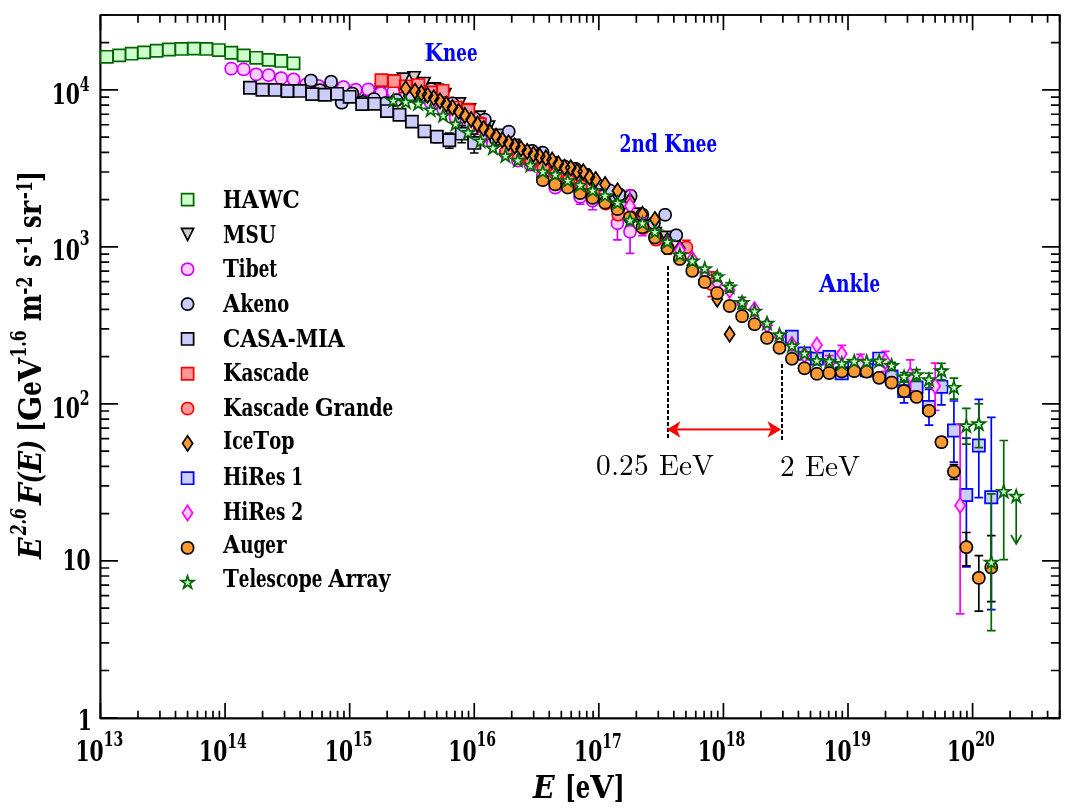
\includegraphics[width=0.7\textwidth]{auger_spectrum_v3.png}
	\caption{Espectro de rayos cósmicos medidos mediante lluvias atmosféricas en función de la energía $E$. Figura obtenida del \emph{Particle Data Group} \cite{PGD}.}
	\label{fig:spectra}
\end{figure}

%%%%%%%%%%%%%%%%%%%%%Check%%%%%%%%%%%%%%%%%%%%%%%%%%%%
Hay diversas teorías detrás del tobillo alrededor de $5 \times 10^{18}\,$EeV en la Fig\,\ref{fig:spectra}. Una teoría dice que el mismo se debe a que una población con un espectro más duro está superando a otra con espectro más blando, por ejemplo un flujo extra-galáctico empieza a dominar sobre un flujo galáctico \cite{bird1994cosmic}. Otra explica que el cambio de la forma de la curva se debe a la pérdida de energía de los protones extra-galácticos, debido al proceso $p\,\gamma \rightarrow\,e^+\,+\,e^-$ conocido como producción de pares con el CMB \cite{berezinsky2006astrophysical}. Una fuerte supresión del espectro para energías por encima de $5\times 10^{19}\,$eV se espera para protones debido a la foto-producción de piones por interacciones con el CMB y para núcleos pesados por foto-desintegración por interacciones con el fondo de radiación infrarrojo. La supresión observada podría deberse a estos procesos, a que las fuentes alcanzan la máxima energía de aceleración o a una combinación de ambos efectos. 
%El proceso para núcleos más pesado es el de foto-desintegración. Para RCs con energías  mayores  a $\nicefrac{E}{A} \geq 6\times 10^{19}\,$eV, el proceso dominante en la pérdida de energía están asociados al efecto GZK \cite{taborda}.
%%%%%%%%%%%%%%%%%%%%%%%%%%%%%%%%%%%%%%%%%%%%%%%%

%%%%%%%%%%%%%%%%%%%Check%%%%%%%%%%%%%%%%%%%%%%%%%%%%%
El flujo de los rayos cósmicos $\Phi$ en función de la energía $E$ puede aproximarse a una ley de potencias que tiene una forma del siguiente tipo
\begin{equation}
	    \frac{d\Phi}{dE} \propto \ E^{-\gamma}   \label{eq:expresion1}
\end{equation}
donde $\gamma$ se lo denomina índice espectral. Este valor varía ligeramente para distintos rangos de energía. Para el rango de energía estudiado en este trabajo, entre 0.25 EeV y 2 EeV como se indica en la Fig.\ref{fig:spectra}, el valor aproximado del índice espectral es $\gamma= 3.27 \pm 0.05$ \cite{data}.


\section{Lluvias atmosféricas extendidas}

%%%%%%%%%%%%%%%%%%%Check%%%%%%%%%%%%%%%%%%%%%%%%%%%%%

{Por encima de una energía de $10^{14}\,$eV, los RCs que llegan a la atmósfera pueden interactuar con las moléculas de la misma,  y así producir cascadas de partículas secundarias. Dependiendo de la energía del primario, es decir el RC que generó la lluvia, estas partículas pueden ser medidas usando detectores sobre la superficie de la Tierra. Esta cascada es conocida como lluvia atmosférica extendida o \emph{EAS} y está compuesta por una componente electromagnética, que consiste en electrones, positrones y fotones, y una componente muónica. Las partículas secundarias cargadas también pueden excitar moléculas de nitrógeno en el aire que producen fotones de fluorescencia y pueden ser observados por telescopios durante noches claras.}

%%%%%%%%%%%%%%%%%%%Check%%%%%%%%%%%%%%%%%%%%%%%%%%%%%
El momento transversal que adquieren las partículas secundarias en el proceso de dispersión a través de la atmósfera es tal que los secundarios se dispersan sobre un área de gran tamaño. Por ejemplo, para energías mayores a 10$\,$EeV,  la lluvia puede llegar a cubrir más de 25\,km$^2$. 

%%%%%%%%%%%%%%%%%%%Check%%%%%%%%%%%%%%%%%%%%%%%%%%%%%
El desarrollo de la lluvia puede describirse mediante la profundidad atmosférica $X(L)$, definida como la masa de aire por unidad de área que atravesó una partícula en su dirección de propagación tras recorrer una distancia $L$, 
\begin{equation}
	X(L)= \int_L^\infty dx \rho(x)
\end{equation}
donde $\rho$ es la densidad del aire en función de la posición.


\section{Descripción de una anisotropía dipolar}
Las anisotropías en las direcciones de llegada de los RCs indican que ciertas zonas del cielo tienen una variación significativa con respecto a la media de flujo de RCs. Estas anisotropías pueden describirse mediante una superposición de funciones armónicas. El primer orden corresponde a una anisotropía dipolar, la misma se puede describir de la siguiente forma:
\begin{equation}
    \Phi(\hat{\bf{u}}) = \Phi_0(1+\bf{d}\cdot\hat{\bf{u}})
    \label{eq:dipolo_general}
\end{equation}
\noindent donde $\Phi_0$ es el flujo medio de eventos, $\hat{\bf{u}}$ es un versor que apunta a la dirección a estudiar, y $\bf{d}$ es un vector con módulo igual a la amplitud del dipolo y cuya dirección está apuntando al máximo del flujo. 

Tomando coordenadas ecuatoriales \footnote{El sistema de coordenadas ecuatoriales se desarrolla en el apéndice \ref{apendice:ecuatorial}}, la dirección de $\bf{d}$ es $(\alpha_d, \delta_d$) y de $\hat{\bf{u}}$ es $(\alpha, \delta)$, entonces  el producto escalar  entre estos vectores se puede escribir de la siguiente manera:
\begin{equation}
    \textbf{d}\cdot\hat{\bf{u}}= d (\cos\delta_d \cos\delta \cos(\alpha - \alpha_d) + \sin\delta_d  \sin\delta)
    \label{eq:product_ud}
\end{equation}

Otro aspecto importante de la representación del dipolo en coordenadas ecuatoriales, es que la proyección de la amplitud del dipolo sobre el plano ecuatorial $d_\perp$ se puede aproximar de la siguiente manera \cite{taborda} :
\begin{equation}
    d_\perp \simeq \frac{r_1}{ \langle \cos\delta \rangle}
    \label{eq:fourier_perp}
\end{equation}
donde $r_1$ es la amplitud del primer armónico en ascensión recta, y $\langle \cos\delta \rangle$ es el valor medio de $\cos\delta $ de los eventos.

\subsection{Representación en coordenadas locales de una anisotropía dipolar}

Podemos reescribir el producto escalar entre el dipolo $\textbf{d}$ y el versor $\hat{u}$ que apunta en una dirección cualquiera mediante las coordenadas locales\footnote{El sistema de coordenadas locales se desarrolla en el apéndice \ref{apendice:local}.}  $\theta$ y $\phi$ como se muestra en la siguiente expresión: 
\begin{align}
    \textbf{d} &=  d_{x'}(\alpha^0, \delta^0)\hat{x}' +  d_{y'}(\alpha^0, \delta^0)\hat{y}'+ d_{z'}(\alpha^0, \delta^0)\hat{z}' \\
    \hat{\bf{u}} &=\sin\theta \cos\phi \hat{x}' + \sin\theta \sin\phi \hat{y}' + \cos\theta\hat{z}'\\
    \textbf{d}\cdot\hat{\bf{u}} &= d_{x'}(\alpha^0, \delta^0)\sin\theta \cos\phi
    + d_{y'}(\alpha^0, \delta^0) \sin\theta \sin\phi  
     + d_{z'}(\alpha^0, \delta^0)\cos\theta \label{eq:dot-prod-local}
\end{align}
donde los versores $\hat{x}'$, $\hat{y}'$ y $\hat{z}'$ apuntan a la dirección Este, Norte y del cenit respectivamente. 

El dipolo $\textbf{d}$ está fijo en el cielo pero visto desde las coordenadas locales, para poder trabajar con $\theta$ y $\phi$, sus proyecciones  $d_{x'}$, $d_{y'}$ y $d_{z'}$ tienen una dependencia con la ascensión recta  $\alpha^0$ y declinación $\delta^0$ del cenit. 

  
\chapter{El Observatorio Pierre Auger}
	\graphicspath{{../02_IntroduccionAuger/}}
	

\section{Introducción}
%%%%%%%%%%%%%%%%%%%Check%%%%%%%%%%%%%%%%%%%%%%%%%%%%%

\textcolor{red}{El observatorio Pierre Auger está ubicado en la ciudad de Malargüe, provincia de Mendoza. El mismo fue construido para detectar las partículas secundarias de las EASs producidas por RCs.  Las propiedades medidas de las lluvias extendidas determinan la energía y la dirección de arribo de cada CR, además de proveer información sobre  la composición de la  misma. El observatorio posee un sistema híbrido de detección, ya que combina un arreglo de detectores de partículas sobre la superficie y un conjunto de telescopios que detectan los fotones de fluorescencia. Cuando el observatorio  registra una EAS que llega a la superficie y reconstruye la dirección de llegada del RC, se dice que se ha detectado un \textit{evento}. La adquisición de datos empezó en el año 2004 y sigue hasta la actualidad.}


\section{Detección de Rayos Cósmicos}
%%%%%%%%%%%%%%%%%%%Check%%%%%%%%%%%%%%%%%%%%%%%%%%%%%
Una característica esencial del Observatorio es la capacidad de registrar lluvias atmosféricas extendidas (EAS) simultáneamente mediante dos técnicas distintas, combinando los detectores de superficie y los detectores de fluorescencia (FD). 

%%%%%%%%%%%%%%%%%%%Check%%%%%%%%%%%%%%%%%%%%%%%%%%%%%

Los análisis presentados en este trabajo fueron realizados con los eventos obtenidos por $ 1660$ detectores Cherenkov, dispuestos sobre de $\sim 3000\,\text{km}^2$ a $1500\,$m entre sí en forma triangular. Un conjunto de 7 detectores adyacentes, es decir una en el medio y 6 en los lados, forman una celda hexagonal o hexágono. Esta disposición de tanques se menciona como \textit{arreglo principal} y se muestra en la Fig.\,\ref{fig:auger_sd}. El conjunto del tanque y la electrónica de detección  se menciona durante este trabajo como \textit{Surface Detector} o \textit{SD}. Además, el Observatorio tiene otro arreglo de SDs separados por $750\,$m llamado \emph{Infill}.

%%%%%%%%%%%%%%%%%%%Check%%%%%%%%%%%%%%%%%%%%%%%%%%%%%
\begin{figure}[H]
	\centering
	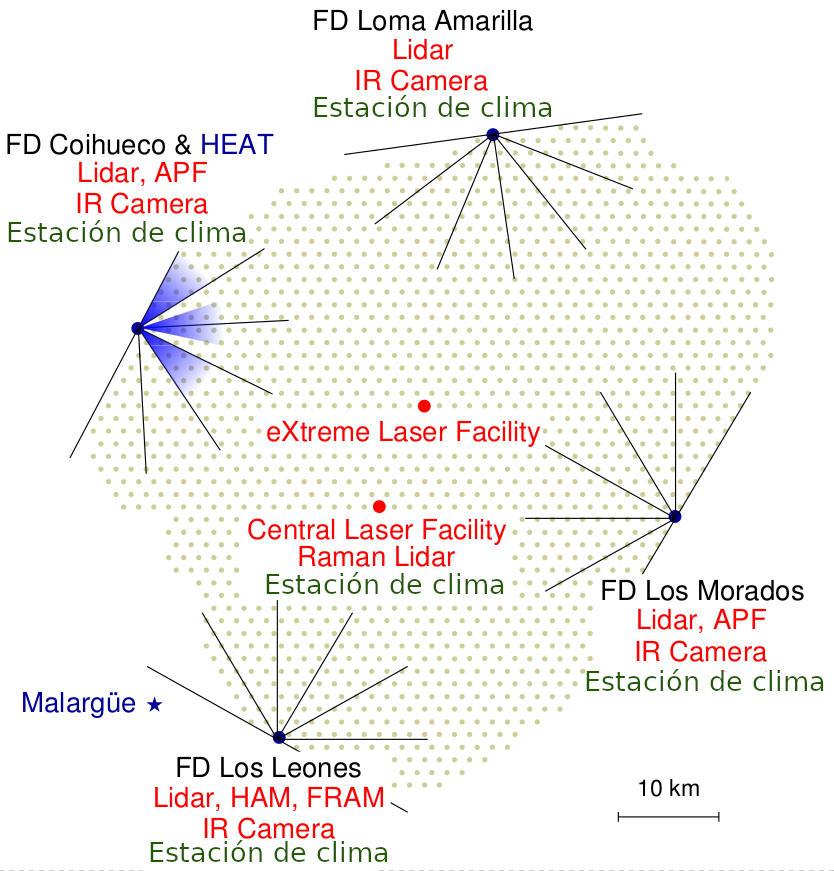
\includegraphics[width=0.7\textwidth]{auger_sd.png}
	\caption{Distribución de los detectores de superficie en el área del Observatorio Pierre Auger. Se muestra la ubicación de las estaciones del clima, otros módulos instalados sobre el observatorio y la posición de los detectores de fluorescencia (FD). Figura de la Colaboración Pierre Auger (2015).}
	\label{fig:auger_sd}
\end{figure}
%%%%%%%%%%%%%%%%%%%Check%%%%%%%%%%%%%%%%%%%%%%%%%%%%%

%%%%%%%%%%%%%%%%%%%Check%%%%%%%%%%%%%%%%%%%%%%%%%%%%%
Los FDs están colocados en cuatro edificios alrededor del arreglo principal: Coihueco, Loma Amarilla, Los Morados y Los Leones indicados en el mapa en la Fig.\,\ref{fig:auger_sd}. Cada edificio contiene 6 FDs, donde cada uno tiene un campo de visión de $30^o\times30^o$, cubriendo así cada uno $180^o$ en la horizontal. Cerca del edificio de Coihueco se encuentran los 3 telescopios del HEAT, los mismos tienen un campo de visión de $60^o$ en el cenit para detectar la máxima profundidad atmosférica de RCs de menor energía.

%%%%%%%%%%%%%%%%%%%Check%%%%%%%%%%%%%%%%%%%%%%%%%%%%%
El área del observatorio es generalmente plana, la altitud de los detectores varía entre $1340\,$m y $1610\,$m, con una altitud media de $\sim1400\,$m. Estos detectores están distribuidos entre las latitudes $35.0^o$ S y $35.3^o$ S y entre las longitudes $69.0^o$ W y $69.4^o$ W.


\subsection{El Detector de Superficie y el Detector de Fluorescencia}
%%%%%%%%%%%%%%%%%%%Check%%%%%%%%%%%%%%%%%%%%%%%%%%%%%
Un detector de superficie (SD), que se muestra en la Fig.\ref{fig:tanque}, consiste en un tanque cilíndrico de polietileno de $3.6\,$m de diámetro y $1.2\,$m de altura con 12 toneladas de agua ultra-pura.  En la parte superior del tanque se encuentran tres foto-multiplicadores (PMT) distribuidos simétricamente a $1.2\,$m respecto al centro del tanque. Los mismos colectan la radiación Cherenkov producida por una partícula cargada relativista que pasa por el agua del detector. \textcolor{red}{El interior está recubierto por una lámina de alta reflectividad para minimizar la pérdida de energía de los fotones por las paredes}. La altura del tanque lo hace sensible a detectar fotones de altas energías, que pueden convertirse en pares electrón-positrón en el volumen de agua \cite{como_funciona_auger}. Cada detector está midiendo constantemente los fotones en el agua, muchos de estos fotones son producidos por ruido y otros por partículas secundarias de una EAS. Los SDs cuentan con algoritmos o reglas para discernir ruido de un evento causado por un rayo cósmico, estos son los algoritmos de disparo que se mencionan en el apartado \ref{triggers_caracteristicas} .

%%%%%%%%%%%%%%%%%%%Check%%%%%%%%%%%%%%%%%%%%%%%%%%%%%
El detector de fluorescencia (FD) y los telescopios del HEAT consisten en 27 telescopios de fluorescencia, esquematizados en la Fig\,\ref{fig:FD}, distribuidos en 4 edificios en los límites del observatorio. Cada telescopio tiene un espejo esférico segmentado de 13$\,m^2$ y una cámara que consiste en 440 PMTs ordenados en una grilla de 22x20. Cada telescopio tiene un campo de visión de $30^o\times30^o$.


\begin{figure}[H]
    \begin{subfigure}[t]{0.45\textwidth}
	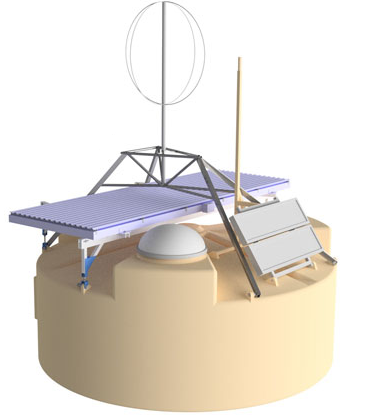
\includegraphics[width=\textwidth]{tanque.png}
	\caption{Detector de radiación Cherenkov con los elementos de la actualización para \emph{Auger Prime}} 	\label{fig:tanque}
    \end{subfigure}%
    \hspace{\fill}
    \begin{subfigure}[t]{0.5\textwidth}
	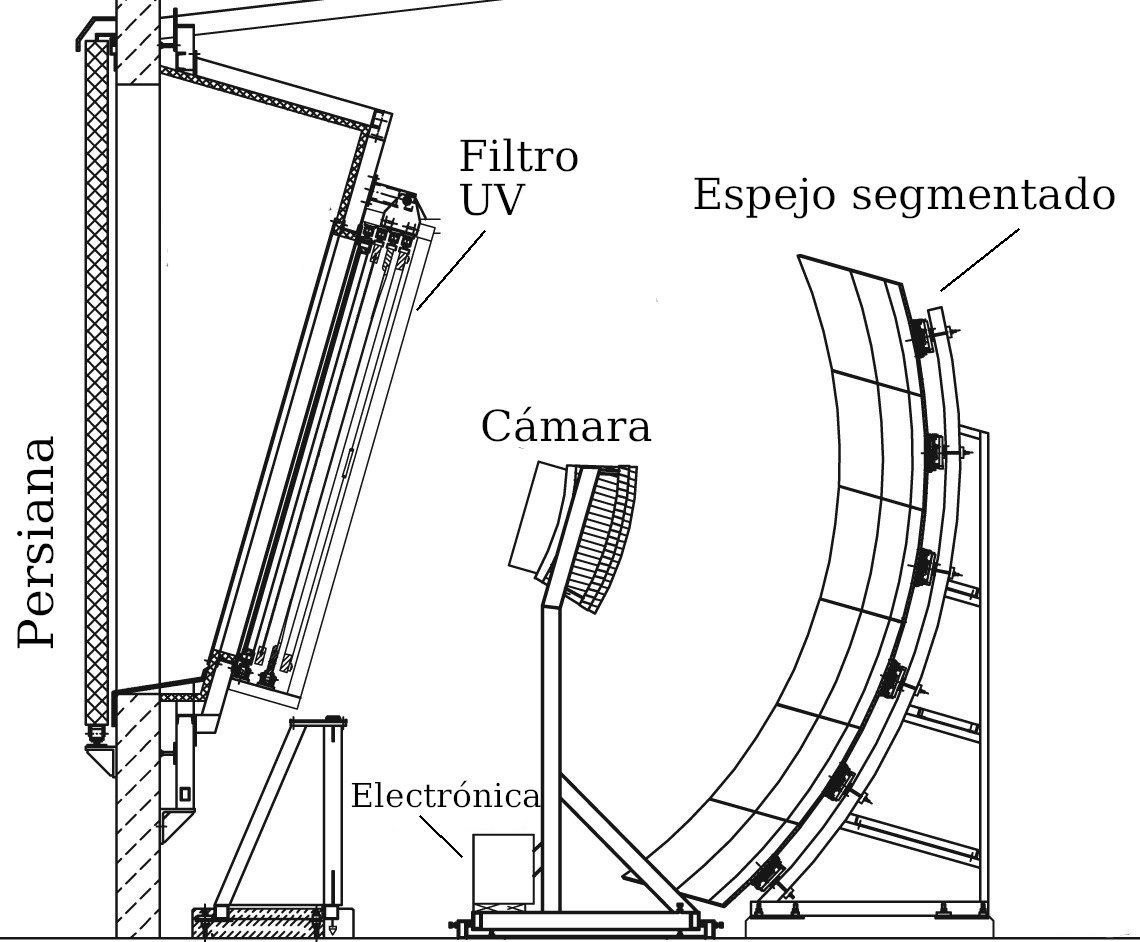
\includegraphics[width=\textwidth]{fd.png}
	\caption{Esquema simplificado de un telescopio de fluorescencia. Extraído de \cite{kit_oracle}}
	\label{fig:FD}
    \end{subfigure}%
    \caption{Detectores empleados por el Observatorio Pierre Auger para la detección de rayos cósmicos.}
	\end{figure}
%%%%%%%%%%%%%%%%%%%Check%%%%%%%%%%%%%%%%%%%%%%%%%%%%%
El FD mide los fotones ultravioletas producidos por la componente electromagnética de la EAS. Mientras se produce la lluvia en la atmósfera, algunos átomos de nitrógeno se excitan y se desexcitan emitiendo fotones. El uso del FD para detectar estos fotones es solo posible en noches sin nubes y sin luna. La posible atenuación de los fotones en la atmósfera es tenida en cuenta para la estimación de la energía, ya que se basa en la cantidad de fotones detectados. Otro factor a tener en cuenta es la presencia de aerosoles, como humo o polvo, esto se realiza midiendo la profundidad atmosférica óptica vertical \emph{Vertical Atmosferic Optical Depth (VAOD)}. Estas mediciones son realizadas por los láseres de las instalaciones de Central Laser Facility (CLF) y de eXtreme Laser Facility (XLF), cuyas ubicaciones se muestra en la Fig.\ref{fig:auger_sd}.

\subsection{Diseño híbrido}\label{seccion:sd_eff}
%%%%%%%%%%%%%%%%%%%Check%%%%%%%%%%%%%%%%%%%%%%%%%%%%%
Los SDs detectan un corte de EAS que llega al nivel del suelo, midiendo las componentes electromagnética y muónica de la lluvia. Cabe resaltar que los SDs funcionan las 24 horas del día, por lo que detectan una mayor cantidad de eventos que el FD. Existen métodos para determinar la dirección de arribo y la energía del primario a partir de estas mediciones.  El SD tiene la propiedad de que la calidad de sus mediciones aumenta con la energía del EAS. 

%%%%%%%%%%%%%%%%%%%Check%%%%%%%%%%%%%%%%%%%%%%%%%%%%%
La exposición se calcula contando la cantidad de hexágonos activos en un tiempo dado, y multiplicado la apertura de un solo SD que vale $4.59\,$km$^2$.sr para lluvias verticales. La exposición instantánea del SD se calcula fácilmente, especialmente para energías mayores a 3 EeV, donde la EAS detectada por cualquier parte del SD es detectada con 100\% de eficiencia independientemente de la masa del primario que inicio la EAS.

%%%%%%%%%%%%%%%%%%%Check%%%%%%%%%%%%%%%%%%%%%%%%%%%%%
El FD es usado para generar una imagen del desarrollo del EAS en la atmósfera. La luz de fluorescencia es emitida isotrópicamente en la parte ultravioleta del espectro, y es producida predominantemente por la componente electromagnética de la lluvia. Los períodos de observación están limitados a las noches sin luna y con buen clima, pero la ventaja del FD es la posibilidad de ver el desarrollo de la lluvia. Dado que la producción de la fotones por fotoluminiscencia es proporcional a la energía depositada en la atmósfera, se puede medir la energía del primario mediante calorimetría. Otro aspecto importante del FD es la posibilidad de medir la profundidad de la atmósfera donde la lluvia alcanza su máximo desarrollo, $X_{max}$, esta cantidad es uno de los más directos indicadores de la composición de masa. \cite{data}

\section{Reconstrucción de eventos de los detectores  de superficie}

\subsection{Selección de eventos}

%%%%%%%%%%%%%%%%%%%Check%%%%%%%%%%%%%%%%%%%%%%%%%%%%%
La reconstrucción de la energía y la dirección de arribo de los CRs se realiza mediante las señales medidas por los SDs. La dirección es reconstruida mediante  el tiempo de llegada de las señales registradas por detectores individuales. Para garantizar la selección de eventos bien contenidos en el SD, se aplica el corte llamado \emph{6T5}. Este corte considera solo a los eventos donde el tanque con mayor señal está rodeado por otros 6 tanques activos. Esta condición asegura una buena reconstrucción de la energía. Al mismo tiempo, este corte simplifica el cálculo de la exposición \cite{exposure}. Para estudios de dirección de arribo pueden utilizar cortes menos estrictos dependiendo del rango de energía a estudiar.

\subsection{Reconstrucción de las lluvias}

%%%%%%%%%%%%%%%%%%%Check%%%%%%%%%%%%%%%%%%%%%%%%%%%%%
En una primera aproximación para la dirección de arribo de la lluvia se obtiene ajustando los tiempos de llegada de la señal en cada tanque. Para eventos con suficientes tanques disparados, estos tiempos de llegada pueden ser descritas como la evolución un frente de lluvia como una esfera que crece con la velocidad de la luz. Los puntos de impacto del EAS con el suelo son obtenidas mediante ajustes a las señales de los tanques. Este ajuste se realiza con un función de distribución lateral (LDF). La LDF también tiene en cuenta la probabilidad de que los tanques no sean disparados y que los tanques con mayor señal estén saturados.

Un ejemplo de la señal que deja un evento sobre el SD 1500 m se muestra en la Fig.\,\ref{fig:evento_sd}. Este evento fue producido por un rayo cósmico de ($104\pm11$)\,EeV con un ángulo cenital de ($25.1\pm0.1 ^o$). La LDF de las señales para este evento se muestra en la Fig.\,\ref{fig:evento_S1000}. La función utilizada para el ajuste de la LDF es una función  $f_{LDF}$ propuesta por Nishimura-Kamata-Greisen \cite{data}
\begin{align*}
	%S(r) = S(r_{opt})\bigg(\frac{r}{r_{opt}}\bigg)^{\beta}\bigg(\frac{r+r_1}{r_{opt}+r_1}\bigg)^{\beta + \gamma}
	S(r) &= S(r_{opt})f_{LDF}(r)\\
	f_{LDF}(r)&=\bigg(\frac{r}{r_{opt}}\bigg)^{\beta}\bigg(\frac{r+r_1}{r_{opt}+r_1}\bigg)^{\beta + \gamma}
\end{align*}
donde $f_{LDF}$ está normalizado tal que $f_{LDF}(r_{opt})=1$ y $r_{opt}$ es la distancia óptima, %$r_1=700\,$m 
y $S(r_{opt})$ es usado para estimar la energía. Para el arreglo SD 1500\,m, el parámetro $r_{opt}=1000\,$m, por lo tanto el tamaño de la lluvia o \emph{shower size} es el valor de S(1000). Dado que la forma de la LDF es desconocida, la forma funcional propuesta para la función $f_{LDF}$ fue elegida empíricamente.  El parámetro $\beta$ depende del tamaño de la lluvia y del ángulo cenital. Los eventos verticales, es decir los eventos con $\theta < 60^o$, son medidas en una etapa menos desarrollada que eventos más inclinados. Los eventos con $\theta>60^o$ atraviesan un mayor cantidad de atmósfera.

\subsection{Calibración de la energía}

Para una energía dada, el valor de S(1000) disminuye para $\theta$ crecientes debido a la atenuación de las partículas de la lluvia. Asumiendo un flujo isotrópico de los CR primarios sobre la parte superior de la atmósfera, se obtiene la atenuación de los datos mostrados en la Fig.\,\ref{fig:s1000_theta}  usando el método de Corte de Intensidad Constante (CIC) \cite{CIC}. La curva de atenuación $f_{CIC}(\theta)$ fue ajustado con un polinomio de orden 3 del tipo $f_{CIC}(\theta)=1+ax+bx^2+cx^3$, donde $x=\cos^2(\theta) - \cos^2(38^o)$. Según lo presentado por la colaboración \cite{collaboration2013pierre}, los valores son $a=0.980\pm0.004$, $b=-1.68\pm0.01$ y $c=-1.30\pm 0.45$, aunque estos coeficientes cambian ligeramente con la energía \cite{data}. El ángulo cenital $\theta=38^o$ se toma como un punto de referencia para convertir S(1000) a S$_{38}$ mediante $S_{38}=S(1000)/f_{CIC}(\theta)$. Este valor S$_{38}$ puede considerarse como la señal S(1000) que hubiera tenido un evento que fue detectado mediante el SD con $\theta=38^o$.


\begin{figure}[H]
	\begin{small}
		\begin{center}
			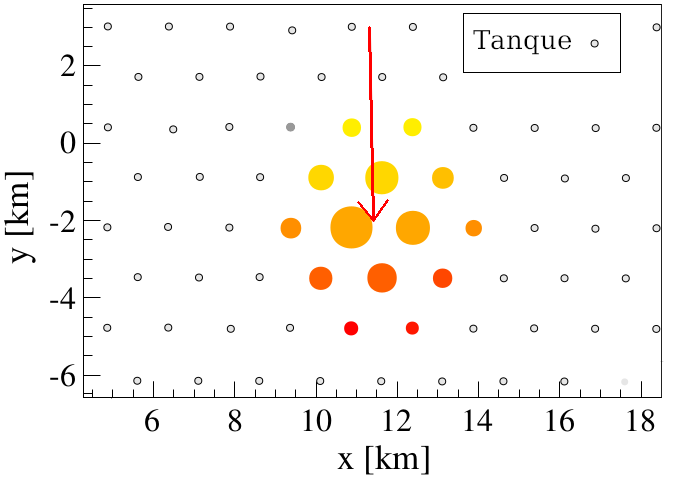
\includegraphics[width=0.65\textwidth]{evento_sd.png}
		\end{center}
		\caption{Ejemplo de la señal dejada por un evento de ($104\pm11$)\,EeV de energía con un ángulo cenital de ($25.1\pm0.1 ^o$) sobre el arreglo principal SD 1500 m. La flecha indica la dirección de arribo de la lluvia. Los colores de los círculo representa el tiempo de arribo de la lluvia, los primeros en amarillo y los últimos en rojo. En área de los círculo pintados es proporcional a logaritmo de la señal. Figura de la Colaboración Pierre Auger (2015). } 	\label{fig:evento_sd}
	\end{small}
\end{figure}


Los eventos con $\theta<60^o$  que fueron detectados por el SD y por el FD son utilizados para relacionar el tamaño de la lluvia con la energía  E$_{FD}$ medida por calorimetría por el FD.  La correlación entre S$_{38}$ y E$_{FD}$ se calcula mediante el método de máxima verosimilitud, que considera la evolución de las incertezas con la energía. La relación entre S$_{38}$ y $E_{FD}$ se describe mediante un función de potencia como se muestra en la Ec.\,\ref{eq:s38_energy}
\begin{equation}
	E_{FD}= A\, (S_{38}/VEM)^B
	\label{eq:s38_energy}
\end{equation}
donde los parámetros obtenidos son $A=(1.86\pm0.03)\times 10^{17}\,$eV y $B=(1.031\pm0.004)$  \cite{tobepublished}. En la Fig.\,\ref{fig:efd_s38} se observa el ajuste y la relación entre  S$_{38}$ y E$_{FD}$


\begin{figure}[H]
	\begin{small}
		\begin{center}
			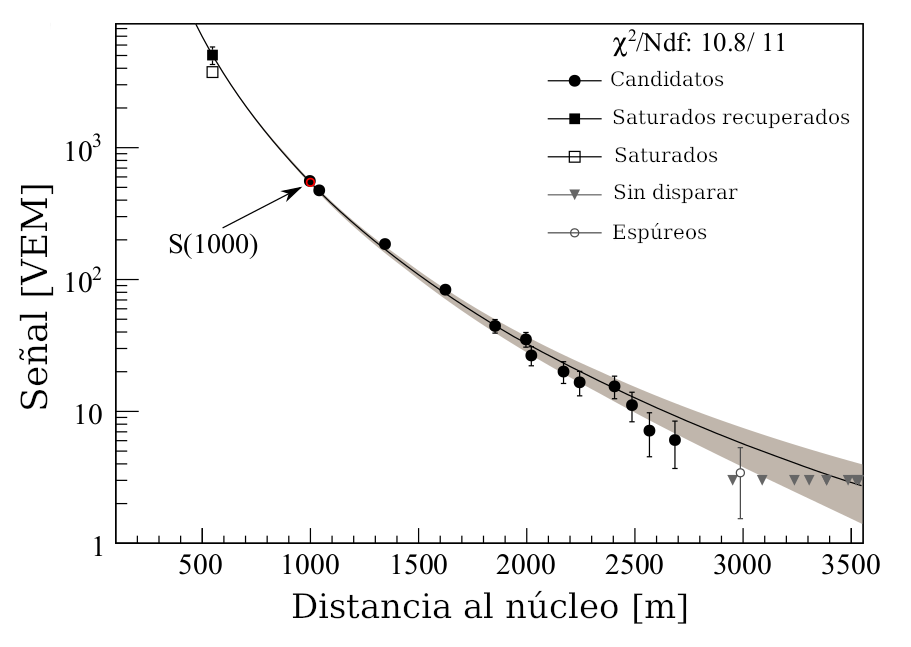
\includegraphics[width=0.65\textwidth]{evento_s1000.png}
		\end{center}
		\caption{Dependencia de la señal con la distancia del núcleo de la lluvia de un evento de ($104\pm11$)\,EeV de energía con un ángulo cenital de ($25.1\pm0.1 ^o$). La función ajustada es la función de distribución lateral (LDF). Del ajuste se obtiene el valor de S(1000). Figura de la Colaboración Pierre Auger (2015). } 	\label{fig:evento_S1000}
	\end{small}
\end{figure}



\begin{figure}[H]
	\centering
	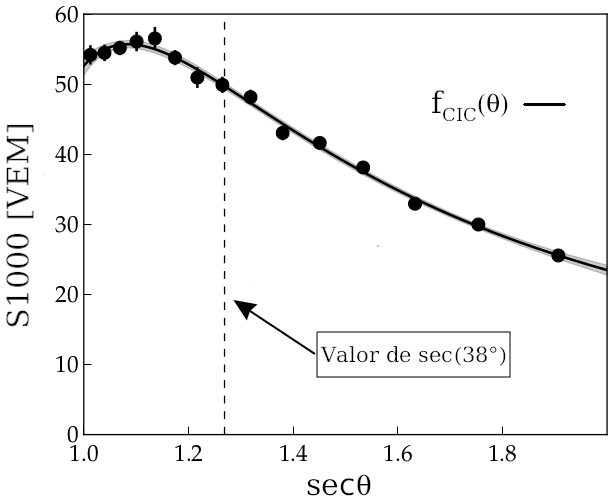
\includegraphics[width=0.6\textwidth]{s1000_theta.png}
	\caption{Curva de atenuación descrita por un polinomio de orden 3. En este ejemplo se deducen los coeficientes de la dependencia del S(1000) a S$_{38}\approx 50\,$VEM que corresponde a un energía de $10.5\,$EeV. Figura de la Colaboración Pierre Auger (2015).} 	\label{fig:s1000_theta}
\end{figure}

\begin{figure}[H]
	\centering
	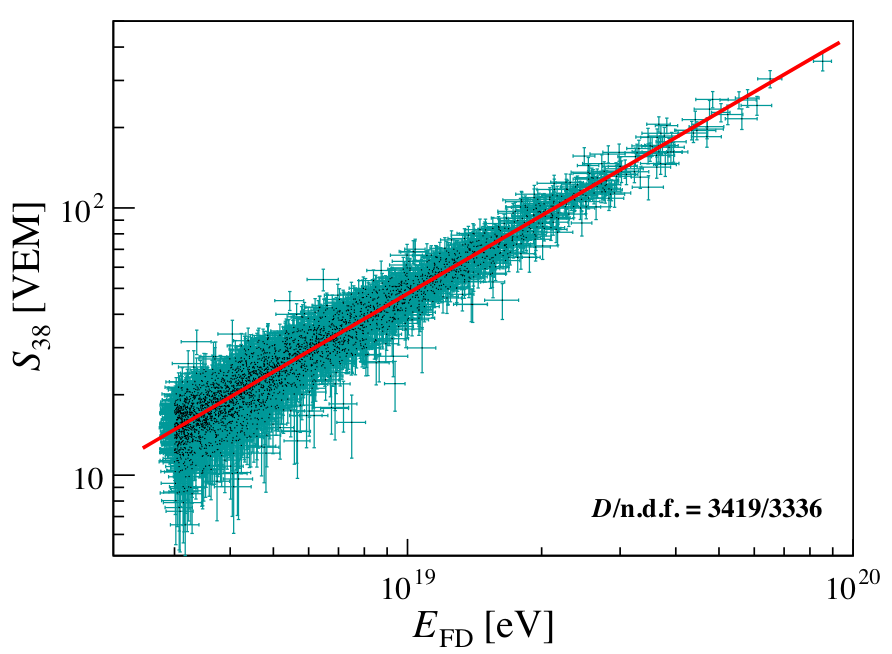
\includegraphics[width=0.67\textwidth]{efd_s38_v2.jpg}
	\caption{Correlación entre el valor S$_{38}$ y la energía $E_{FD}$ medida por el FD. Con estos datos se ajustan los parámetros A y B que relacionan la señal y la energía.  Figura de la Colaboración Pierre Auger (2020).} 	\label{fig:efd_s38}
\end{figure}


\subsection{Monitoreo del clima}\label{seccion:clima}

Las condiciones atmosféricas, como la temperatura, presión y humedad, se deben tener en cuenta para estudiar el desarrollo de los EAS, así como también para estudiar la cantidad de fotones de las lluvias sobre los moléculas de N$_2$, emitidos por fluorescencia. Distintas estaciones monitorean las condiciones atmosféricas sobre el Observatorio Pierre Auger, cuatro cerca  de los edificios donde se encuentran los FD y uno cerca del centro del SD 1500\,m. Para este trabajo se utilizaron las mediciones de la presión y temperatura registradas la mayor parte del tiempo en la estación del clima cerca del CLF, la misma realiza una medición cada intervalo de 5 minutos la mayor parte del tiempo. Cuando no se cuenta con datos registrados para intervalos entre 10 minutos hasta 3 horas, en estos casos se utiliza una interpolación de los datos medidos. Si el período de tiempo es mayor a 3 horas, los eventos durante este periodo no son considerados para la determinación de los efectos del clima en la señal detectada por el SD 1500\,m.

	\graphicspath{{../03_IntroduccionReport/}}
	\section{Algoritmos de disparo del detector de superficie} \label{triggers_caracteristicas}

\subsection{Disparo Estándar}

El disparo ToT o \emph{Time over Threshold} está diseñado para adquirir datos de una duración relativamente larga, de esta manera se puede distinguir señales producidas por EASs por encima del ruido, ya que el último consiste en picos más cortos. Las señales producidas por un evento tienen un decaimiento exponencial con una constante de $70\,$ns, que es el tiempo de decaimiento de la luz dentro del tanque. Los PMTs registran señales en intervalos de $25\,$ns, por lo que una señal alta puede ser registrada durante varios periodos de adquisición de datos. Si por algún motivo, ya sea ruido u otro evento dentro de la ventana del disparo, se produce otro pico durante el decaimiento de la señal de evento puede cumplir la condición de disparo con una mayor señal que la que le corresponde.

{El eventos comúnmente presentados en los trabajos de la Colaboración Auger son registrados con un algoritmo de disparo ToT que se menciona como \emph{Disparo Estándar}.  Estos eventos son medidos utilizando un algoritmo cuya eficiencia varía con la energía del CR. Para el Disparo Estándar, los eventos con energía mayor a $3\,$EeV y ángulo cenital $\theta<60^o$ o  por encima de $4\,$EeV y $\theta<80^o$, son detectados con una eficiencia del 100\%. Por lo tanto, el análisis en el rango de energía entre $1\,$EeV - $2\,$EeV requiere factores relacionados con la eficiencia del disparo en función de la energía. Estos factores son obtenidos de manera fenomenológica \cite{taborda}.}


A medida que los tanques pasan más tiempo midiendo van perdiendo sensibilidad a los eventos de bajas energías. Esto es una desventaja del Disparo Estándar en los SDs en el rango $1\,$EeV - $2\,$EeV.  En la Fig.\ref{fig:futuro}, para los datos presentados en el ICRC 2019, se observa como la cantidad de eventos para energía menores a $3\,$EeV va disminuyendo, además la energía media de los eventos para distintos rangos de tiempo va aumentando.

 
\subsection{Todos los Disparos}

Para recuperar la sensibilidad para bajas energías, a partir del año 2013  se implementan otros algoritmos de disparo en los SDs, llamados ToTd y MoPS \cite{pierre2013plans}. Estos algoritmos de disparo se mencionan en este trabajo como \textit{Todos los Disparos}. A comparación del Disparo Estándar o ToT, el algoritmo ToTd hace una deconvolución del pico medido por el PMT. De esta forma se acelera la caída exponencial de la señal de un evento, y la reduce a uno o dos periodos de  $25\,$ns con una señal alta, seguida de varios picos con valores negativos \cite{ToTd}. En el caso de MoPS, el mismo cuenta la  cantidad de aumentos sucesivos en la señal detectada por el PMT en una ventana de tiempo dado. La condición de disparo se cumple si esta cantidad de aumentos sucesivos está por encima de cierto número \cite{MoPS}. El algoritmo MoPS es más sensible a las señales electromagnéticas, que son anchas en tiempo, en cambio el algoritmo ToTd es sensible a los picos de corta duración.  

% We first define apositive stepin a FADC trace as a cumulation of successive increases.  Thisis illustrated in Fig.1, where the positive steps are indicated by blue arrows.  Their valuesare  integer  by  definition.   The  MoPS  algorithm  consists  in  counting  how  many  positive steps exceed a certainthresholdThwithin a slidingwindowof a certain lengthW, and to require this number to be above a certainoccupancyvalueM.  So, the parameters definingthe trigger condition are similar to those defining the ToT trigger, except that hereThisdirectly defined in FADC units, not as a given fraction of a calibrated VEM value.
% suppresses the exponentialtail of an elementary signal and reduces it to one or two slots with high amplitude, followedby a tail of positive or negative values
% In case of the MoPS the trigger probability reaches a plateau of about 50\% asby design it is not sensitive to narrow peaks but to the spread electromagnetic signals

En la Fig.\ref{fig:TLD} se observa como la cantidad de eventos para energía menores a $2\,$EeV va disminuyendo como el caso del Disparo Estándar pero en una menor proporción con respecto a los eventos registrados con eficiencia completa.


\begin{figure}[H]
	\centering
	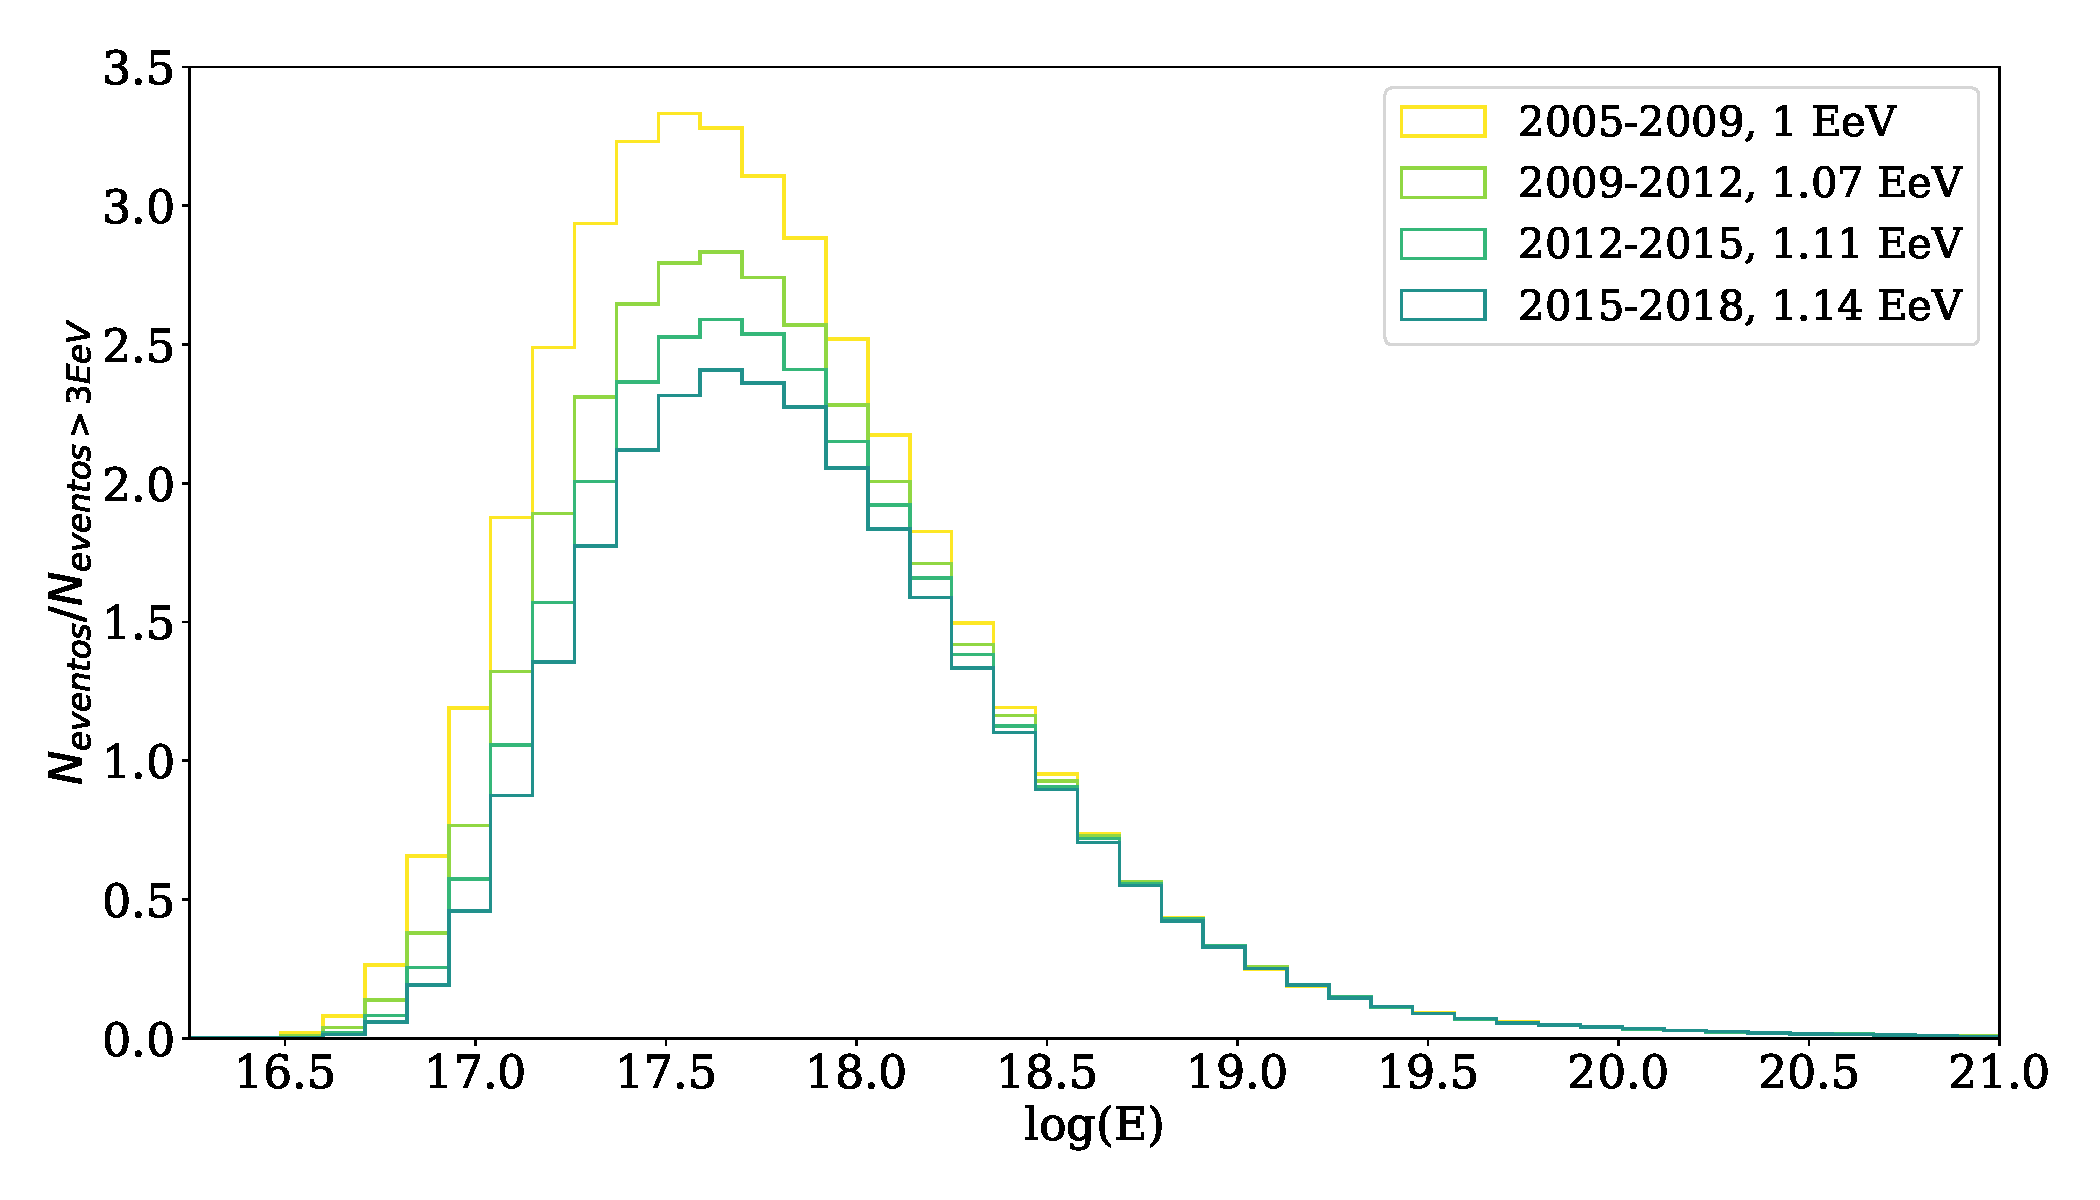
\includegraphics[width=0.8\textwidth]{histograma_Standard.pdf}
	\caption{Histograma de eventos  del Disparo Estándar por rango de tiempo medido por el Observatorio Pierre Auger}
	\label{fig:futuro}
\end{figure}


\begin{figure}[H]
	\centering
	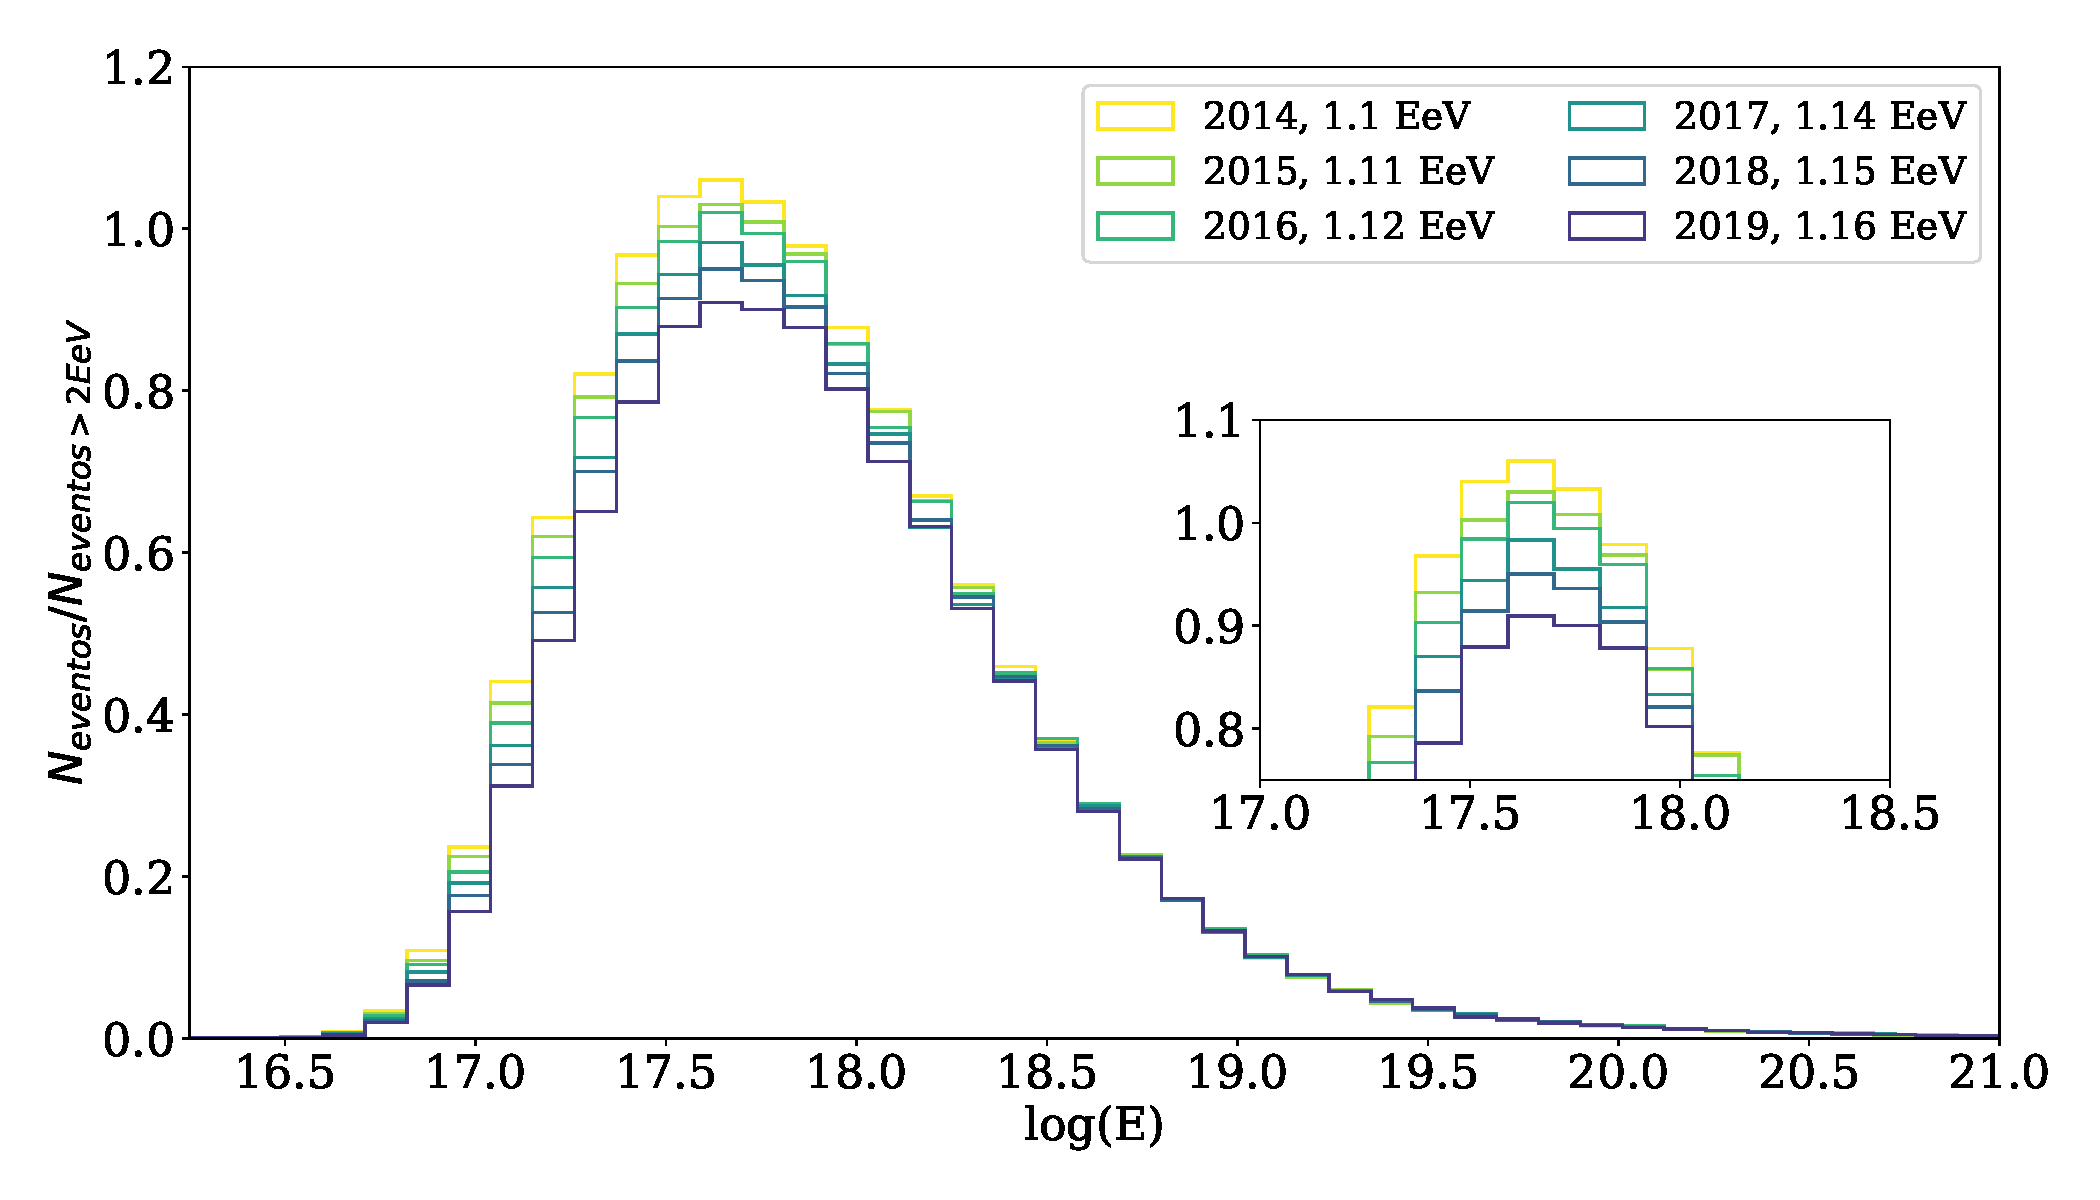
\includegraphics[width=0.8\textwidth]{histograma_AllTriggers.pdf}
  \caption{Histograma de eventos de  Todos Los Disparos por rango de tiempo medido por el +
  Observatorio Pierre Auger}
	\label{fig:TLD}
\end{figure}

La implementación de los ToTd y MoPS fue llevada a cabo mediante una actualización de la electrónica de los SDs para bajar el umbral de disparo, en particular para las señales de la componente electromagnética de la EAS, mejorando así la reconstrucción de eventos mediante la separación fotón/hadrón para bajas energías  \cite{pierre2013plans}. Con esta mejora, el umbral de eficiencia completa para Todos los Disparos es menor que el Disparo Estándar, este umbral es de una energía de $1\,$EeV. En la Fig\,\ref{fig:triggers} se comparan las eficiencia del Disparo Estándar y Todos los Disparos en función de la energía del evento. De tal manera que, al estudiar los eventos en el rango $1\,$EeV - $2\,$EeV,  no son necesarios los factores de eficiencia y sólo pueden afectar los cambios de la exposición direccional del Observatorio.


\begin{figure}[H]
  \centering
  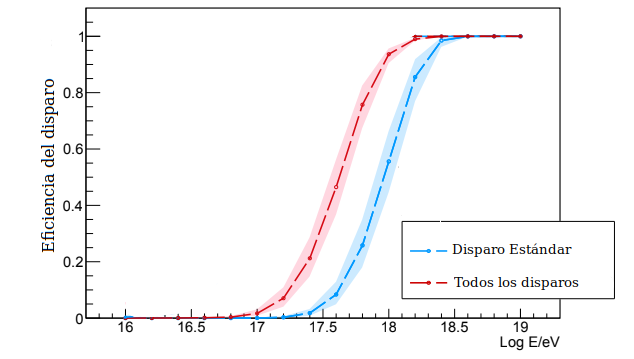
\includegraphics[width=0.75\textwidth]{comparacion_triggers.png}
  \caption{La eficiencia del disparo en función de la energía para eventos con ángulo cenital $\theta$ menor a $60^o$. Esta figura fue extraída de un trabajo interno de la Colaboración {\cite{triggers_ref}}.}
  \label{fig:triggers}
\end{figure}


Una desventaja de Todos los Disparos sobre el Disparo Estándar, es que el último tiene una mayor cantidad de años medidos, ya que se adquieren datos  desde el año 2004 con este algoritmo. Esto es conveniente ya que mientras más años han sido medidos es más factible que los efectos espúreos se cancelen. En cambio, para Todos los Disparos, el análisis  es posible desde el año 2013. Entre inicios del 2004 y finales del 2019, el conjunto de eventos del Disparo Estándar tiene $6\,975\,194$ eventos sin clasificar, es decir todos los eventos registrados por el Observatorio sin discriminar por energía. En cambio entre mediados del 2013 hasta fines del 2019, el archivo de eventos para Todos los Disparos tiene $13\,739\,351$ eventos sin clasificar, por lo que el menor tiempo de medición se compensa con la eficiencia del disparo.


\section{Acerca de los eventos utilizados en este trabajo} \label{filtro}

Se aplican cortes a los eventos para asegurar la eficiencia completa de los detectores. Estos cortes implican límites en ángulo cenital $\theta$ de los eventos, en la cantidad de vecinos al tanque de mayor señal, además de restringirse a eventos medidos en condiciones normales, es decir, cuando los sistemas de comunicación del Observatorio funcionan sin inconvenientes. De esta manera, podemos prescindir de otros factores de corrección.

A partir de los registros de eventos del arreglo principal con Todos los Disparos, se consideran solamente los eventos que cumplan las siguientes características:

    \begin{enumerate}
      \item La calidad de la reconstrucción depende de la energía y del ángulo cenital $\theta$ del evento.  Para el Disparo Estándar los eventos por debajo de los $4\,$EeV, se consideran los eventos con $\theta < 60^o$, en cambio para eventos por encima de esta energía se consideran hasta $\theta < 80^o$. Para Todos los Disparos se consideran solo los eventos con $\theta<60^o$.
      \item Los datos del evento son recopilados sin inconvenientes. Este filtro se conoce como \emph{Bad period flag} o $ib$. Un valor de 1 indica un buen periodo. Con este filtro se descartan eventos debido a probables fallas de alimentación o problemas de comunicación o adquisición que podrían inducir errores en el análisis.
      \item Buena reconstrucción de la lluvia atmosférica asociada al evento.
      \item El tanque de mayor señal está en el interior de un hexágono de tanques activos. Estos eventos se conocen como \textit{eventos 6T5}.
    \end{enumerate}


\subsection{Acerca del registro de hexágonos}\label{hexagonos_rate}

La cantidad de celdas  activas sobre el Observatorio está relacionado con el filtro de eventos $6T5$, que garantiza la calidad de la reconstrucción del evento. El Observatorio lleva un registro de la cantidad de hexágonos activos cada 5 min, además de registrar las condiciones atmosféricas en distintas estaciones de clima sobre la superficie del Observatorio. 

% #@@@@@@@@@@@@@@@@@@@@@@@@@@@@@@@@@@@@@@@@@@@@@@@@@@@@@@@@@@@@
% #@@@@@@@@@@@@@@@@@@@@@@@@@@@@@@@@@@@@@@@@@@@@@@@@@@@@@@@@@@@@
% #@@@@@@@@@@@@@@@@@@@@@@@@@@@@@@@@@@@@@@@@@@@@@@@@@@@@@@@@@@@@
% #@@@@@@@@@@@@@@@@@@@@@@@@@@@@@@@@@@@@@@@@@@@@@@@@@@@@@@@@@@@@
% \section{Acerca de la tesis de licenciatura}

% Durante la tesis de licenciatura se analizaron los efectos de las condiciones atmosféricas durante el desarrollo de las EAS.  Se analizaron los datos adquiridos durante en el periodo 2005-2018 por el arreglo principal. De esta manera, se extendió los periodos estudiados anteriormente en los siguientes trabajos \cite{abraham2009atmospheric}, \cite{abreu2012description}   y \cite{aab2017impact}. 

% Los efectos atmosféricos afectan principalmente a la atenuación de la componente electromagnética  de la EAS, en particular depende fuertemente de la temperatura y presión. Estos efectos  se caracterizan por parámetros dependientes del ángulo cenital del evento y por la presión, densidad y temperatura al momento de su detección. Los parámetros mencionados se utilizan para corregir las señales registradas por los SDs. Las correcciones del clima utilizadas por la colaboración Pierre Auger fueron implementadas a partir del trabajo \cite{aab2017impact} en el 2017. 

% Durante el trabajo de la licenciatura se reprodujo el análisis de la modulación del clima sobre el periodo 2005-2015 del trabajo \cite{aab2017impact}, obteniéndose resultados compatibles. También se estudió la modulación del clima mediante el valor de la señal medida por los SDs, $S_{38}$, sin la corrección propuesta por \cite{aab2017impact}, además de extender el rango de tiempo analizado hasta el 2018. Se observó que los parámetros del clima obtenidos en este análisis sobre  $S_{38}$  son compatibles con los utilizados en la reconstrucción oficial. 

\chapter{Modulación del clima sobre los datos del Observatorio Pierre Auger}

	\graphicspath{{../04_Clima/}}
	% Para el análisis y ajuste se trabajó con dos conjuntos de datos distintos. El primero fue el conjunto de datos que la colaboración Pierre Auger presentó en la Conferencia Internacional de Rayos Cósmicos (ICRC) del año 2015, este conjunto de datos se utilizó para el cálculo de las correcciones climáticas al estimador de energía \cite{aab2017impact}. El segundo conjunto de datos se presentó en la ICRC del año 2019. Entre estos dos conjuntos de datos existieron cambios en la reconstrucción de energía de los eventos, en particular en el valor de la señal de S$(1000)$ \cite{isabel}, además de agregar la corrección por las modulaciones del clima propuesto en \cite{aab2017impact} sobre este mismo valor de señal y se implementó una función de corte de intensidad constante CIC que varía en función de la energía. El objetivo de este capítulo es comprobar si la corrección del clima de la reconstrucción de eventos es adecuada.

\section{La física detrás de la modulación del clima}\label{seccion:fisica_clima}

El arreglo principal mide las 24 horas del día las lluvias de partículas que llegan al suelo. Las señales registradas por los WCDs, ya sea mediante la componente electromagnética o muónica de las EAS, se usan para determinan la posición del núcleo, la dirección de arribo del CR y la energía del primario. La señal de los eventos son ajustados mediante un función de distribución lateral (LDF) para obtener una señal de referencia $S(1000)$. Existieron cambios en los parámetros de la LDF y, por lo tanto, de valor de $S_{38}$, utilizado para estimar la energía del primario. La conversión de $S(1000)$ a $S_{38}$ se realiza mediante el método de corte de intensidad constante (CIC) explicado anteriormente. Además en la nueva reconstrucción el CIC es función de la energía.

\subsection{Trabajos anteriores}

Debido a la modulación del clima dependiente de la estaciones, es de esperarse encontrar una modulación diaria y anual sobre la cantidad de eventos observados por el SD. Ya que en días con menor densidad y presión atmosférica, los tanques detectan eventos por debajo del umbral con mayor facilidad. Este fenómeno fue estudiado por trabajos anteriores realizados por la colaboración Pierre Auger \cite{aab2017impact} \cite{collaboration2009atmospheric}. En particular, el trabajo \cite{aab2017impact} consideró el retraso que tienen los cambios de  la temperatura a distintas alturas sobre la superficie, como se muestra en la Fig\,\ref{fig:delay} que son datos del GDAS (Global Data Assimilation System) promediados por hora del día. Posteriormente esta corrección fue implementada en el proceso  de análisis de datos del observatorio.


En la Fig.\,\ref{fig:delay} se observa que los ajustes realizados a las variaciones de la temperatura  según la hora del día con una función del tipo $T(t) = T_{media} + A\times \sin((t-t_d)\nicefrac{\pi}{12\,\text{hs}})$.  En la Tabla\,\ref{tabla:delay} se observa que entre 1400\,m (altitud del observatorio Pierre Auger) y la mayor altitud medida por el GDAS existe un corrimiento de $2.1\pm0.7\,$hs.

Como la relación entre la densidad y la temperatura del aire están relacionadas mediante la expresión $\rho \approx \nicefrac{0.3484P}{T +273.16}\,$kgm$^{-3}$, con P en hPa y T en  $^o$C \cite{aab2017impact}, el corrimiento de la temperatura al aumentar la altitud también se ve reflejada en la densidad. Como la misma es una variable importante para el desarrollo de la cascada en al atmósfera, este retraso debe tenerse en cuenta.

\begin{figure}[H]
	\centering
	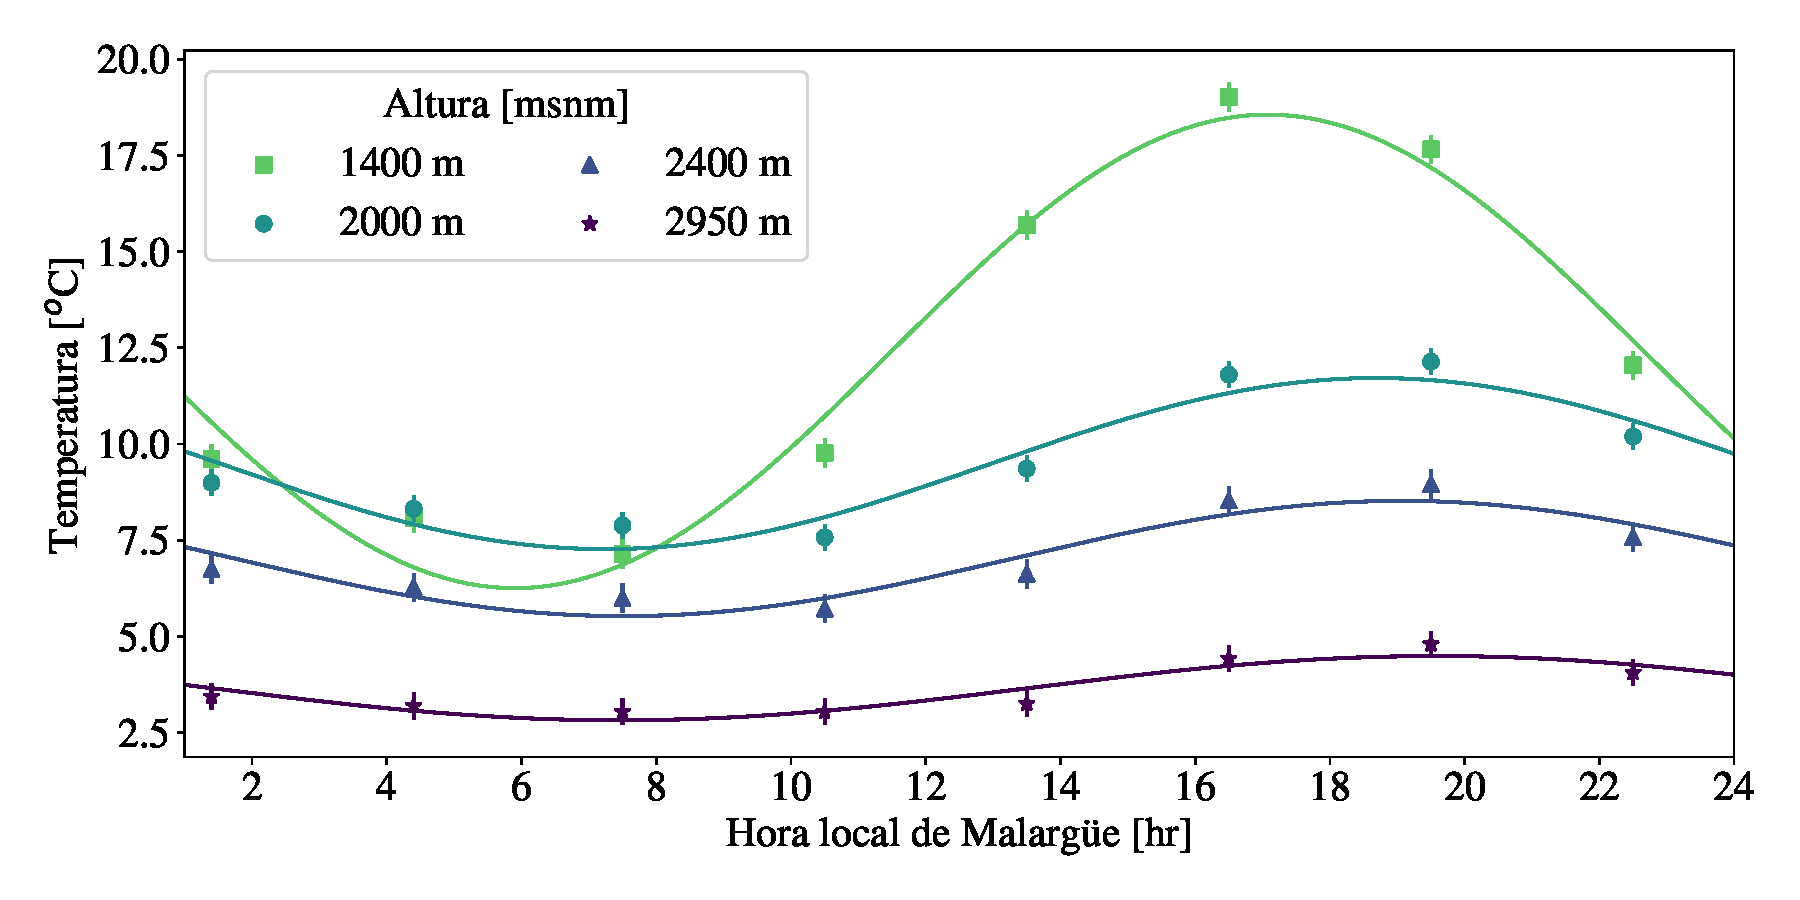
\includegraphics[width=0.8\textwidth]{delay_v2.pdf}
	\caption{Mediciones de la temperatura a distintas alturas sobre el nivel del mar en función de la hora del día en Malargüe. (Hora Local: GMT-3).}
	\label{fig:delay}
\end{figure}
\begin{table}[H]
\centering
\begin{tabular}{c|c|c|c}
	\multirow{2}{*}{\begin{tabular}[c]{@{}c@{}}Altura \\ {[}msnm{]}\end{tabular}} & \multirow{2}{*}{\begin{tabular}[c]{@{}c@{}}T$_{media}$ \\ {[}$^o$C{]}\end{tabular}} & \multirow{2}{*}{A {[}$^o$C{]}} & \multirow{2}{*}{t$_d$ {[}h{]}} \\
																				  &                                                                                                      &                                                 &                                \\ \hline
	1400                                                                          & $12.4\pm0.5$                                                                                         & $5.6\pm0.6$                                     & $12.5\pm0.5$                   \\ \hline
	2000                                                                          & $9.5\pm0.2$                                                                                          & $2.1\pm0.3$                                     & $10.8\pm0.6$                   \\ \hline
	2400                                                                          & $7.0\pm0.2$                                                                                          & $1.4\pm0.2$                                     & $10.7\pm0.6$                   \\ \hline
	2950                                                                          & $3.7\pm0.1$                                                                                          & $0.8\pm0.1$                                     & $10.4\pm0.6$                   \\ 
	\end{tabular}
\caption{Características de la modulación de la temperatura en función de la altura sobre el nivel del mar.}\label{tabla:delay}
\end{table}

\subsection{Efectos de la atmósfera sobre los rayos cósmicos}

La variación de las condiciones atmosféricas afecta las señales de las lluvias atmosféricas extendidas. Estas señales pueden ser detectadas en la superficie por un arreglo de detectores, como los que se encuentran en el Observatorio Pierre Auger. Estos efectos pueden inducir errores sistemáticos en la reconstrucción de energía de los rayos cósmicos. Se han realizado  trabajos anteriores sobre los efectos del clima sobre la señal detectada en el Observatorio Pierre Auger \cite{collaboration2009atmospheric} \cite{aab2017impact}. En este trabajo se estudió eventos con energía mayor a $1\,$EeV entre los años 2005-2018, extendiendo los periodos de tiempo estudiados anteriormente.
%444444444444444444444444444

Para entender los parámetros utilizados para describir a la lluvia, debemos entender que son la longitud de radiación $X_0$, la profundidad de la lluvia $X_{max}$ y el radio de Molière $r_M$. La longitud de radiación definida como $X_0=\nicefrac{d}{2}$,  donde $d$ es un parámetro que indica cuanta cantidad de materia debe atravesar un partícula cargada relativista para perder un factor de $\approx 50\%$ de su  energía. El $X_0$ depende del material que atraviesa la partícula, y tiene unidades de [g\,cm$^{-2}$]. La profundidad de la lluvia $X_{max}$ de una cascada puramente electromagnética, i.e. iniciada por un fotón, tiene la siguiente expresión \cite{matthews2005heitler}
\begin{equation}
 	X_{max} = X_0{ln(\frac{E}{\xi^e_c})}
 \end{equation} 
donde  $\xi^e_c$ es la energía crítica para la cual las pérdida de energía por radiación supera a la pérdida de energía por colisión, en el aire $\xi^e_c=85\,$MeV. Por último, el radio de Molière $r_M$ que puede expresarse como 
\begin{equation}
	r_M= \frac{E_s}{\xi^e_c}\frac{X_0}{\rho}
\end{equation}
es la máxima profundidad transversal que alcanza la lluvia. El valor de $E_s\approx21\,$MeV caracteriza las pérdidas por dispersión. Usualmente un cilindro con un radio $r_M$ contiene al 90\% de la energía depositada en la atmósfera por el primario. El radio de Molière local en el aire para una altura $h$ puede definirse como $r_M = \nicefrac{9.6\,\text{gcm}^{-2}}{\rho(h)}$ \cite{gora2006universal}. 
%444444444444444444444444444

Las variables atmosféricas importantes que afectan al desarrollo de la EAS en la atmósfera son la presión y la densidad del aire. Por un lado la presión es una medida de cantidad de materia que atraviesa el CR. Si la presión sobre la superficie aumenta implica que la lluvia va a atravesar más partículas, y por el contrario si la presión disminuye la lluvia tiene menos materia para interactuar. Esto afecta el desarrollo longitudinal de la lluvia cuando llega a la superficie. En la Fig.\,\ref{fig:eas} se muestran una esquema simplificado de las interacciones en al atmósfera de un primario de la misma energía. En la figura de la izquierda representa la lluvia donde la presión y la densidad está por encima de la media, y la figura de la derecha representa un lluvia donde la presión y la densidad de la atmósfera están por debajo de la media.

\begin{figure}[H]
	\centering
	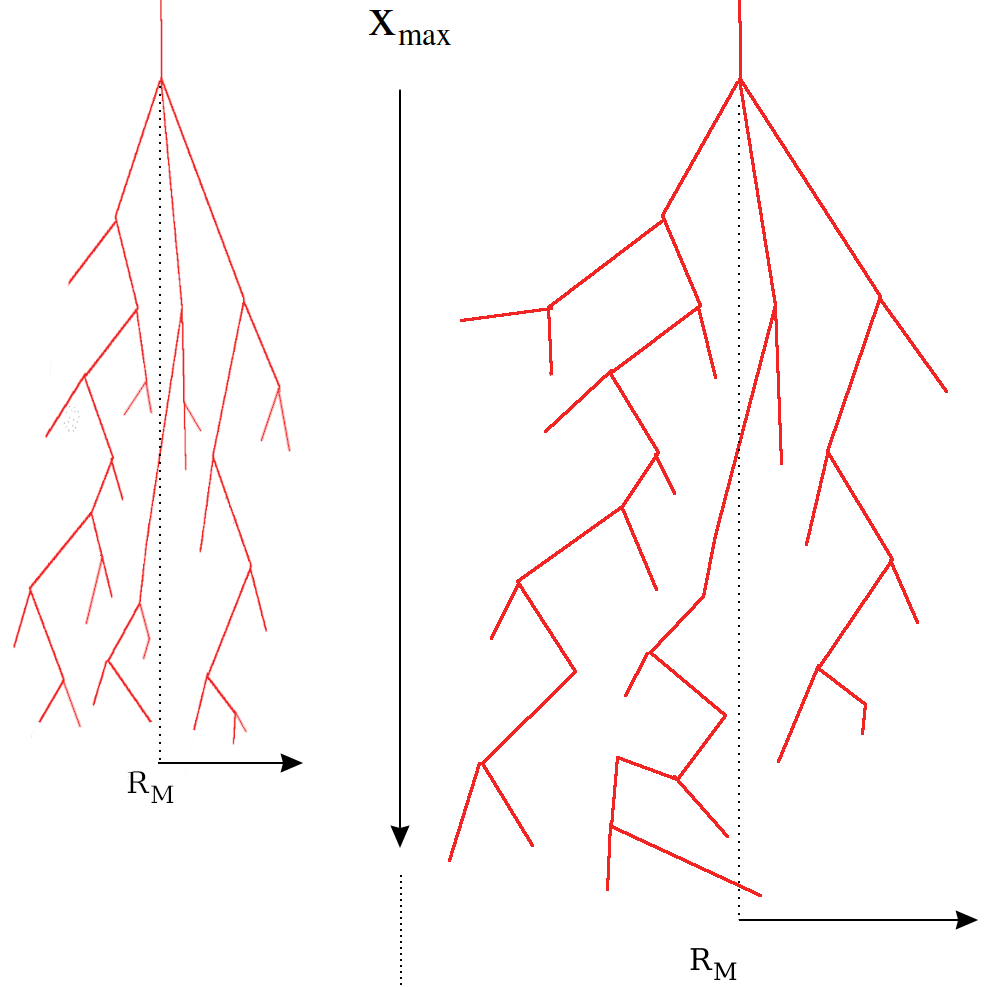
\includegraphics[width=0.5\textwidth]{eas.png}
	\caption{Diagramas simplificado de un lluvia de la misma energía para distintas condiciones atmosféricas}
	\label{fig:eas}
\end{figure}

Estos efectos se ven reflejados en la señal sobre el SD del Observatorio Pierre Auger. La extensión de la señal sobre el SD, es decir el $r_M$ puede cambiar según la densidad de la atmósfera por encima del SD. Los valores de $r_M$ relevantes para la señal medida son a nivel del suelo y a 1000 m. Esto implica que las variaciones de densidad (o de temperatura) a estas alturas están relacionadas con las variaciones al nivel del suelo. La variación a $\sim2400\,$m sobre el nivel del mar está atrasada dos horas con respecto a la variación sobre el Observatorio, que se encuentra a $\sim1400\,$m sobre el nivel del mar. Otro aspecto importante es que la amplitud de está variación disminuye con la altura. Entre las dos altitudes mencionadas existen una relación de aproximadamente $\nicefrac{1}{3}$ entre las amplitudes. 

\subsection{Descripción del modulación en la señal medida}

Considerando lo analizado en \cite{aab2017impact} \cite{collaboration2009atmospheric}, en este trabajo se propone la siguiente modulación, presentada en la Ec.\,\ref{eq:signal}, para la señal S que reciben los tanques 
\begin{equation}
	S=S_0\big(1+\alpha_P(P-P_0) +\alpha_{\rho}(\rho_{media}-\rho_0) + \beta_{\rho}(\rho_{2h}-\rho_{media})\big)
	\label{eq:signal}
\end{equation}
donde $S_0$ es la señal  del evento en condiciones atmosféricas medias, $P$ es la presión en el momento del evento, $P_0=862\,$hPa es la presión media en el rango de tiempo estudiado, $\rho_{media}$ es la densidad  media del aire en 24\,hs, $\rho_0=1.06\,$kgm$^{-3}$ es la densidad media durante el periodo estudiado, $\rho_{2h}$ es la densidad que se midió dos horas antes del evento  y los coeficientes $\alpha$ y $\beta$ tiene en cuenta la modulación del clima sobre la señal.  Si consideramos la tasa $R_{ang}$  por ángulo sólido $\Omega$

\begin{equation}
	\frac{dR_{ang}}{d\Omega} = \int_{S_{min}}^{\infty} P_{Tr}(S,\theta) d\Phi_{CR}
	\label{eq:rate_angular}
\end{equation}
donde $P_{Tr}$ es la probabilidad de que sea detectado un evento para un valor de señal mínimo $S_{min}$ dado, y $\Phi_{CR}$ es la densidad de eventos por ángulo sólido. La función $P_{Tr}$ tiene en cuenta la eficiencia del disparo de los tanques en función de la energía. Por ejemplo, para el SD 1500 m, como se mencionó anteriormente, la eficiencia máxima de disparo es a partir  de $3\,$EeV. Considerando  las Ecs.\,\ref{eq:s38_energy} y \ref{eq:expresion1} , se puede reescribir la Ec.\ref{eq:rate_angular} como integral de la señal medida S. Teniendo en cuenta que la corrección del clima es pequeña podemos escribir la Ec.\,\ref{eq:signal} como $S=S_0(1+\epsilon)$ y las Ecs. \ref{eq:expresion1} y \ref{eq:s38_energy}.
\begin{align*}
\frac{d\Phi_{CR}}{dE} 	&\propto E^{-\gamma} 					\qquad\qquad\qquad\qquad\qquad \quad \qquad \qquad		\frac{dE}{dS}  			= \frac{dE}{dS_0}\,\frac{dS_0}{dS}\\ 
					  	&= S^{-B\gamma}(1+\epsilon)^{B\gamma}    \qquad\qquad \qquad\qquad\qquad \qquad 				  	 = AB\,S^{B-1}\, (1+\epsilon)^{-B}\\
   		    			\frac{dR_{ang}}{d\Omega} &= \int_{S_{min}}^{\infty} P_{Tr}(S,\theta) \frac{d\Phi_{CR}}{dE} \frac{dE}{dS} dS\\
    						 &\propto \int_{S_{min}}^{\infty} P_{Tr}(S,\theta) \bigg( S^{-B\gamma}(1+\epsilon)^{B\gamma}\bigg) \bigg( AB\,S^{B-1}\, (1+\epsilon)^{-B}\bigg)dS\\
    						 &\propto A\,B (1+\epsilon)^{B\gamma - B}\int_{S_{min}}^{\infty} P_{Tr}(S,\theta) S^{-B\gamma +B -1} dS
\end{align*}

Dado que $\epsilon\,\ll\,1$, uno puede expandir la expresión $(1+\epsilon)^{B\gamma}$ hasta primer orden 
\begin{equation*}
	(1+\epsilon)^{B\gamma-B} \approx 1 + B(\gamma-1)\epsilon
\end{equation*}
Por lo que la expresión final queda de la siguiente forma
\begin{equation*}
	\frac{dR_{ang}}{d\Omega} \propto AB(1+B(\gamma - 1)\epsilon)\int_{S_{min}}^{\infty} P_{Tr}(S,\theta) S^{-B\gamma +B -1} dS
\end{equation*}

Considerando que $d\Omega= sin(\theta)d\theta d\phi$ y que el área efectiva  que tiene el observatorio para dado un evento con ángulo cenital $\theta$ es $M_{eff}=M\times cos(\theta)$, donde $M$ es el área activa del observatorio en el momento del evento. Podemos definir la tasa de eventos por área $R$ como
\begin{align*}
	dR 	&\propto \frac{dR_{ang}}{d\Omega} \frac{M_{eff}}{M} d\Omega \\
		&\propto \frac{dR_{ang}}{d\Omega}\, cos(\theta)\, sin(\theta)\,d\theta d\phi\\
		%&=  AB(1+B(\gamma - 1)\epsilon)\, cos(\theta)\, sin(\theta)\,d\theta d\phi \int_{S_{min}}^{\infty} P_{Tr}(S,\theta) S^{-B\gamma +B -1} dS\\
		&\propto  AB(1+B(\gamma - 1)\epsilon)\,d\sin^2\theta d\phi\,\int_{S_{min}}^{\infty} P_{Tr}(S,\theta) S^{-B\gamma +B -1} dS
\end{align*}

Así pudiendo definir la tasa por área por $sin^2(\theta)$, independiente del valor de $\phi$

\begin{align*}
	\frac{dR}{d(sin^2\theta)} &\propto AB(1+B(\gamma-1)\epsilon)\, 2\pi \,\int_{S_{min}}^{\infty} P_{Tr}(S,\theta) S^{-B\gamma +B -1} dS
\end{align*}

Los parámetros $\alpha_P$, $\alpha_{\rho}$ y $\beta_{\rho}$ podrían depender del ángulo cenital o de la energía (por ende de S). En este trabajo se considera solamente la dependencia en $\theta$. Si $P_{Tr}$ es independiente de $\theta$, podemos absorber estas constantes y dejar la expresión como

\begin{equation}
	\frac{dR}{d(sin^2\theta)} = R_0\bigg[1+a_P(P-P_0) +a_{\rho}(\rho_{media}-\rho_0) + b_{\rho}(\rho_{2h}-\rho_{media})\bigg] 
	\label{eq:rate_sin2}
\end{equation}
donde los parámetros $a_P=B(\gamma-1)\alpha_{P}$, $a_{\rho}=B(\gamma-1)\alpha_{\rho}$ y $b_{\rho}=B(\gamma-1)\beta_{\rho}$, donde los parámetros B y $\gamma$ son conocidos.

\subsection{Estimador del ajuste}

Para determinar los parámetros del clima, se calcula la tasa de eventos por hora durante un periodo seleccionado normalizada con el área correspondiente a ese momento. Durante el trabajo se menciona la tasa de eventos, pero debe tenerse en cuenta que es la tasa normalizada con el área. Esta área es calculada a partir de la cantidad de hexágonos activos. Por lo tanto, una vez obtenida la tasa, se ajusta la misma mediante la expresión de la Ec.\ref{eq:rate_sin2}, obteniéndose los parámetros del clima.

Para realizar este ajuste, se supone que el número de eventos observado en una hora sigue una distribución de Poisson. Se realiza un ajuste de máxima verosimilitud (\emph{Maximum Likelihood Estimator}) para estimar los coeficientes del clima de la Ec.\ref{eq:rate_sin2}. La función a minimizar tiene la siguiente expresión 
\begin{equation}
	L=\prod_i\frac{\mu_i^{n_i} e^{-\mu_i}}{n_i!}
\end{equation}
donde $\mu_i$ es la media de la distribución de Poisson, que es el número de eventos esperado durante una hora que puede calcularse como
\begin{equation}
	\mu_i = R_0A_iC_i
\end{equation}
donde $R_0$ es la tasa promedio que se observaría si los parámetros atmosféricos fueran los de referencia, es decir $R_0=\nicefrac{\sum n_i}{\sum A_iC_i}$, donde $A_i$ es el área efectiva en el intervalo de tiempo $i$ y el parámetro $C_i$ tiene la forma

\begin{equation}
	C_i = 1+a_P(P-P_0) +a_{\rho}(\rho_{media}-\rho_0) + b_{\rho}(\rho_{2h}-\rho_{media}) 
\end{equation}
con $\rho_{2h}$, como fue mencionado anteriormente, es la densidad medida dos horas antes del evento. Es posible que estos coeficientes dependan de la energía, por ejemplo por la dependencia del logaritmo de la energía de $X_{max}$ o por los cambios de composición a distintas energías. En todo caso, se espera que estas dependencias sean pequeñas.

\subsection{Condiciones climáticas y área activa del observatorio Pierre Auger}

Existen tres estaciones meteorológicas dentro del observatorio, que miden cada 5 minutos las condiciones climáticas en distintos puntos. Las ubicaciones de estas estaciones están indicadas en la Fig.\,\ref{fig:auger_sd}. Las Figs.\,\ref{fig:clima_p} y \ref{fig:clima_p_rho} se muestran las variaciones de los valores de presión y densidad en el periodo del $2005-2018$ con respecto a la media en este mismo periodo. En las mismas se observa las modulación anual de la densidad, Fig.\,\ref{fig:densidad_hora}, y al modulación diaria de la densidad, Fig.\,\ref{fig:area_auger}, que afecta a la detección de las lluvias por parte del SD. 

Para asegurarse eventos con una buena reconstrucción de  energía, posición del núcleo y dirección de arribo, solo los eventos que están contenidos dentro del arreglo del SD son considerados. Este criterio requiere que el detector con mayor señal esté rodeado de 6 tanques activos. Teniendo en cuenta la geometría de arreglo de WCDs, se calcula el área efectiva mediante la suma del área asociada a cada tanque. El mismo contribuye un área de $\sqrt{3} \frac{d^2}{2}$, donde $d$ es la distancia entre WCDs en una grilla triangular. Como la cantidad de hexágonos activos varía con el tiempo también lo hace  el área efectiva del observatorio. En la Fig.\,\ref{fig:area} se muestra la evolución del área efectiva del SD 1500 m hasta el año 2018. La línea horizontal  limita el área mínima considerada para el análisis. Estos periodos de baja exposición no proveen información suficiente para caracterizar la modulación.
Este valor de corte en el área corresponde aproximadamente al $10\%$ del valor nominal.

\begin{figure}[H]
	\centering
		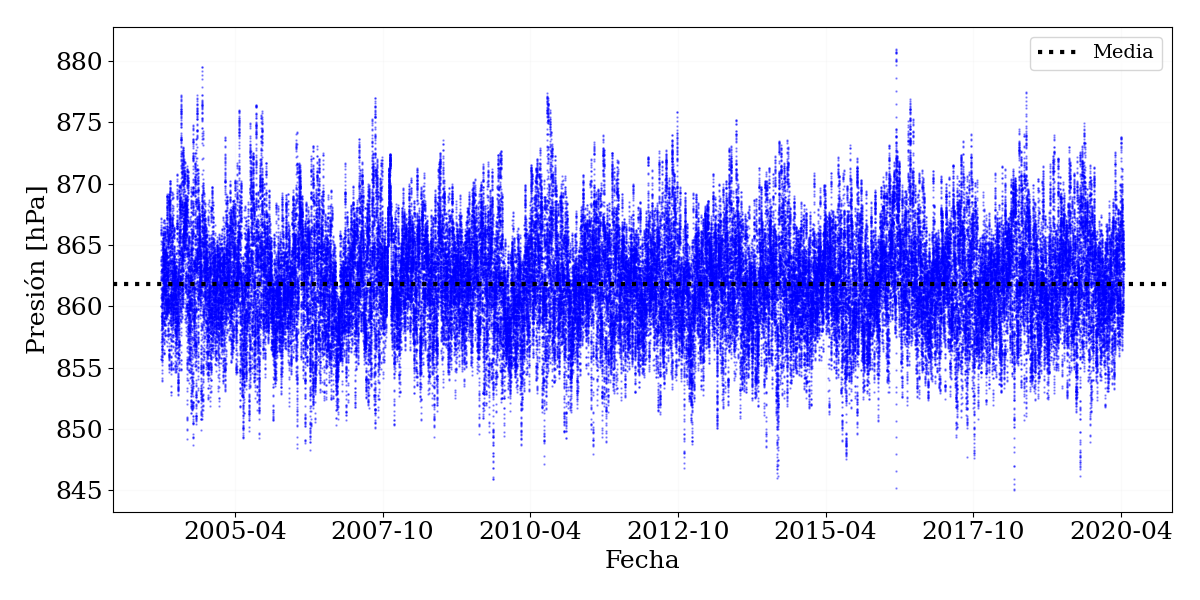
\includegraphics[width=0.8\textwidth]{Graphs/clima/presion_v2.png}
	\caption{Variación de la presión sobre el Observatorio en función del tiempo}
  \label{fig:clima_p}
\end{figure}


\begin{figure}[H]
	\centering
        \begin{subfigure}[b]{0.8\textwidth}	
			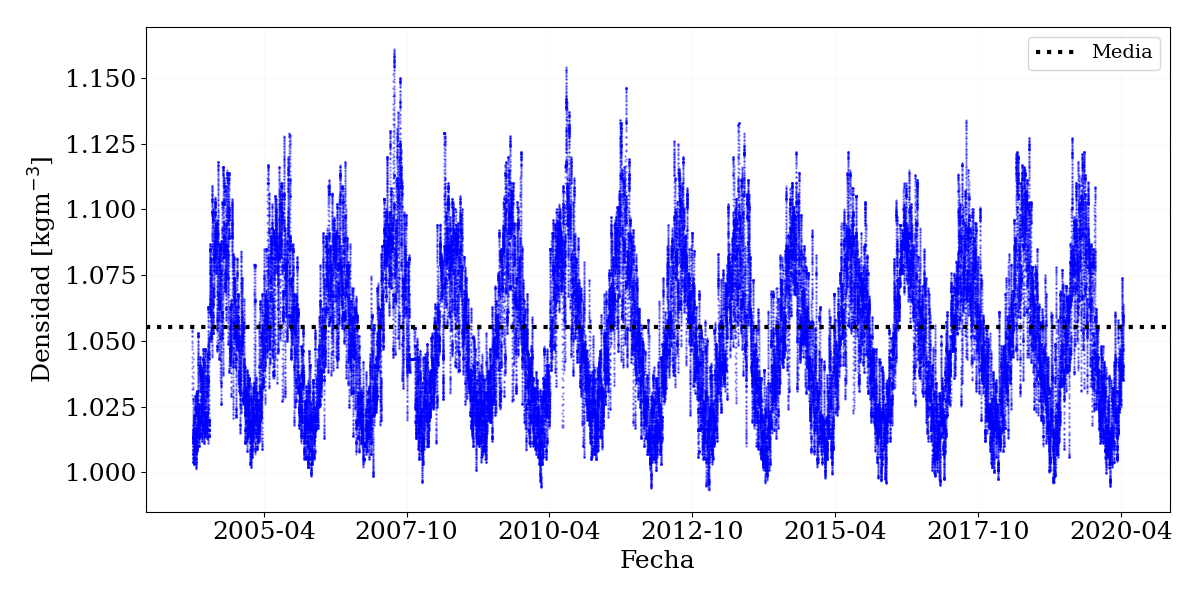
\includegraphics[width=\textwidth]{Graphs/clima/densidad_diaria_v2.png}
			\caption{Densidad diaria}
			\label{fig:densidad_diaria}
        \end{subfigure}\\
        % \hspace{\fill}
        \begin{subfigure}[b]{0.8\textwidth}
			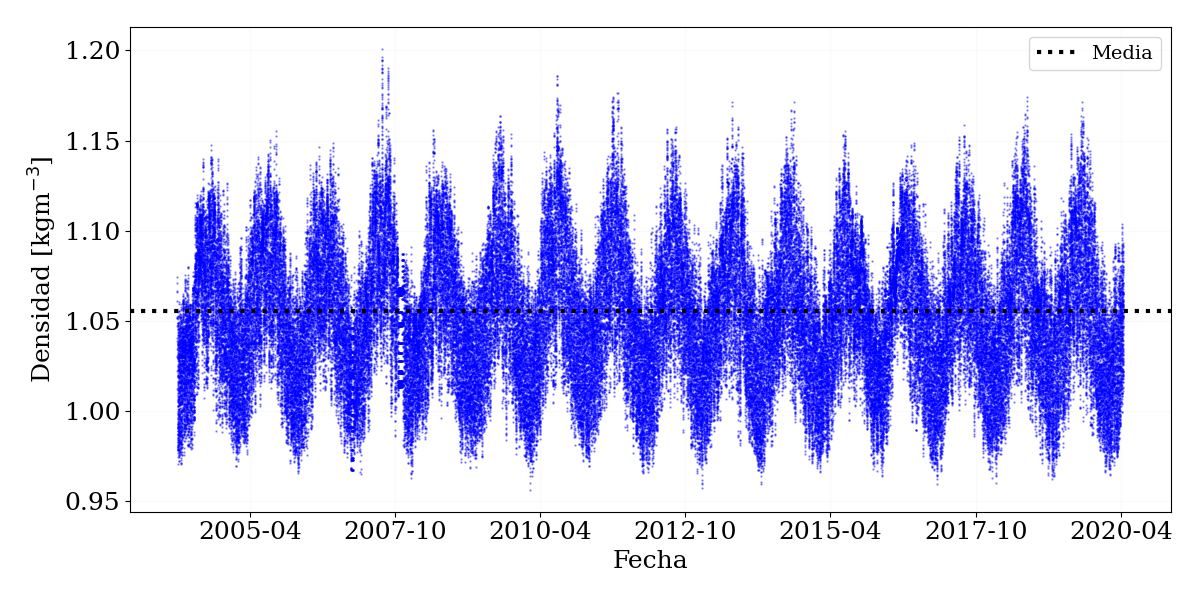
\includegraphics[width=\textwidth]{Graphs/clima/densidad_media_diaria_v2.png}
			\caption{Densidad media por hora}
			\label{fig:densidad_hora}
		\end{subfigure}\\
		% \hspace{\fill}
        \begin{subfigure}[b]{0.8\textwidth}	
			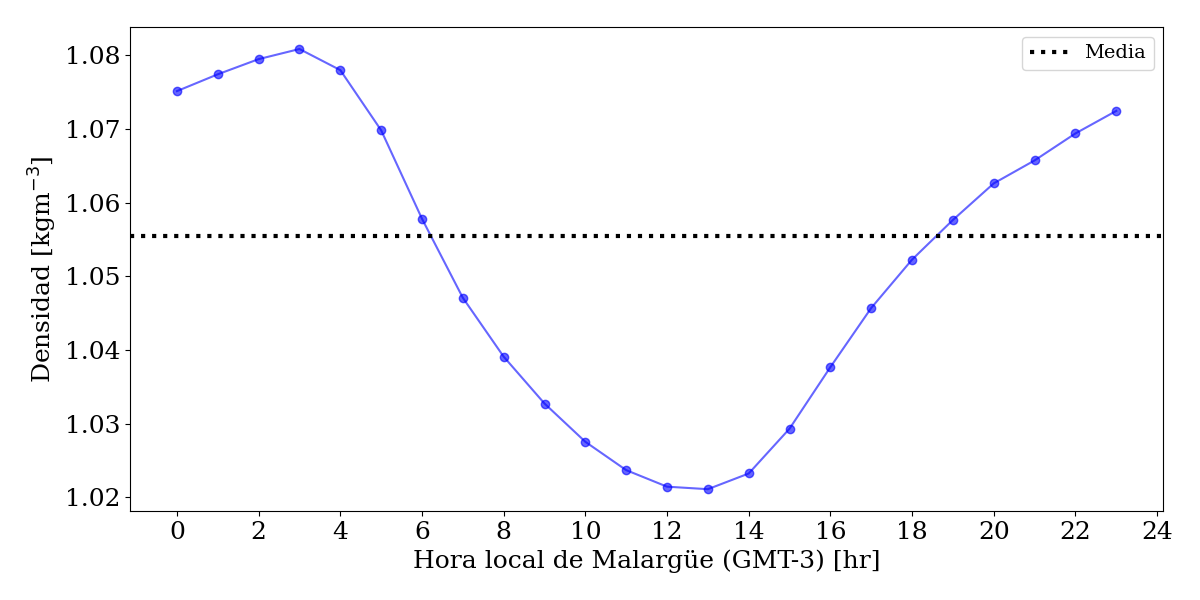
\includegraphics[width=\textwidth]{Graphs/clima/densidad_hod_v2.png}
			\caption{Densidad media por hora del día.}
			\label{fig:area_auger}
        \end{subfigure}\\
  \caption{Variaciones de las variables del clima en función del tiempo}
  \label{fig:clima_p_rho}
\end{figure}

En este trabajo se utilizan los datos recabados por las estaciones del clima del observatorio. Como se menciona en la sección \ref{seccion:clima}, existen periodos donde los datos del clima son interpolados. Es por ello que se consideran los eventos registrados durante un periodo en donde las condiciones climáticas fueron medidas o interpoladas para un periodo menor a 3 horas.

\begin{figure}[H]
    \centering
    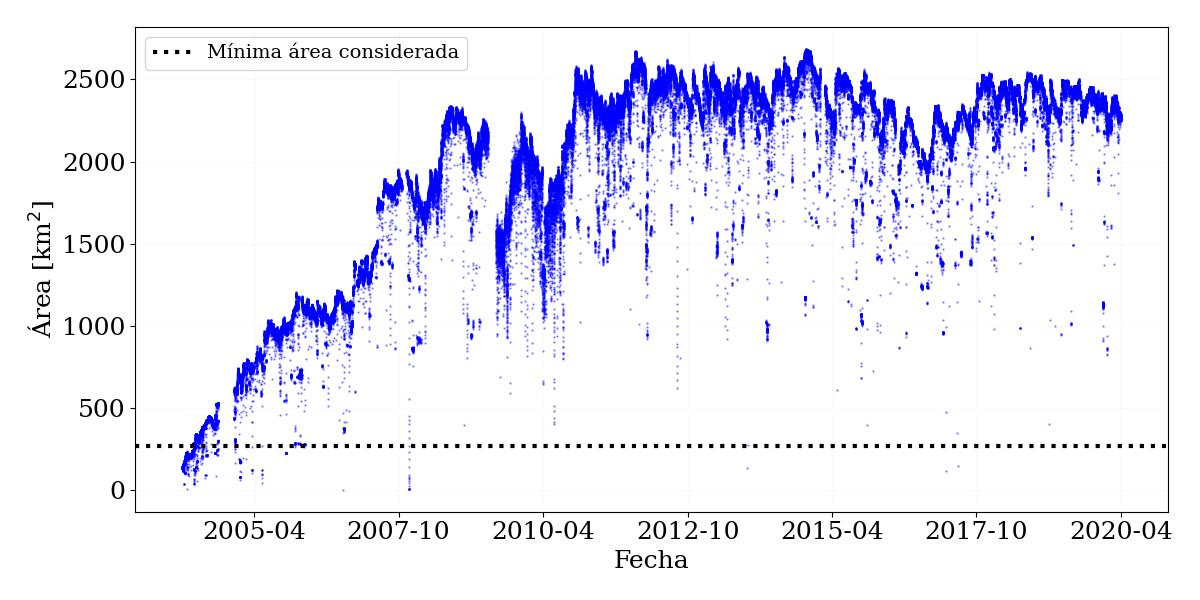
\includegraphics[width=0.8\textwidth]{Graphs/clima/area_v2.png}
    \caption{Evolución temporal del área efectiva del Observatorio Pierre Auger. La línea horizontal señala el área mínima considerada para el análisis.}
    \label{fig:area}
\end{figure}


	
%|SD 1500
% \section{Resultados para el arreglo principal}
\section{Eventos asociados al Disparo Estándar en el rango 2004-2018}\label{Stan_modulacion}	
	
En esta sección se trabajó con los conjuntos de datos  presentados en la ICRC 2015  y  en la ICRC 2019 registrados por el arreglo principal con el Disparo Estándar. La señal de $S(1000)$ del conjunto del ICRC 2019 fue corregida en la reconstrucción oficial de eventos por la modulación del clima, por los parámetros obtenidos en \cite{aab2017impact}. 

En este trabajo se emula el análisis de datos realizado en \cite{aab2017impact} con los datos del ICRC 2017, con el fin de verificar que se obtienen los mismos resultados. Luego se realizó un análisis similar con los datos de nueva reconstrucción de la señal $S_{38}$ sin la corrección del clima  del conjunto de datos de la ICRC 2019 en el periodo 2005-2018. 

Los coeficientes atmosféricos se obtienen tomando una energía mayor a $1\,$EeV en el caso de los datos de la ICRC 2015. Para el caso del análisis con el valor de $S_{38}$ de la ICRC 2019, se realiza el corte de eventos con el valor de $S_{38}$  que tiene un evento de $1\,$EeV.  



	
%====|==>ICRC 2015	
\subsection{Datos presentados en la ICRC 2015}\label{icrc2015}

Se utilizaron los datos de la ICRC 2015 utilizando los cortes recomendados mencionados en la sección anterior. Además de considerar eventos con energía mayor a $1\,$EeV en un periodo de tiempo entre el 1 de Enero del 2005 y 31 de Diciembre del 2015, y con ángulo cenital $\theta$ menor que $60^o$.  Tras los cortes mencionados, se analizaron $1\,146\,470$ eventos con una la media de energía de $2.00\,$EeV. Nos referiremos a este subconjunto de datos del ICRC 2015  como conjunto A. Las características de estos datos se resumen en la Tabla \ref{tabla:caracteristicas_ICRC_2015}.
%====|====|	Tabla de eventos exposure
        \begin{table}[H]
            \centering
            \begin{tabular}{r|c|} \cline{2-2}
                & ICRC  2015 \\ \cline{2-2}
            Inicio:              & 01/01/2005 \\ 
            Final:               & 01/01/2016  \\ 
            Número de eventos:   & $1\,146\,470$ \\ 
            Energía media:       & 2.00\,EeV    				\\ 
            Corte en energía:    & $> 1$ EeV        				\\ 
            Corte en ángulo cenital:		& $\theta < 60^o$ 				\\ \cline{2-2}
            \end{tabular}
        \caption{Características de los datos ICRC 2015 utilizados para el cálculo de los parámetros del clima de esta sección. } \label{tabla:caracteristicas_ICRC_2015}
        \end{table}

% ====|====|Tabla del fit
        Se realiza un ajuste de la tasa de eventos por hora del conjunto A para obtener los coeficientes promediados por ángulo cenital, que incluye todos los eventos de ángulo cenital $\theta< 60^o$. Los parámetros obtenidos se presentan y se comparan con \cite{aab2017impact} en la Tabla \ref{tabla:parametros_ICRC_2015}. Los errores presentados son los errores obtenidos por el ajuste. El $\chi^2_\nu$ representa el $\chi^2$ reducido, que para este ajuste es de $\chi^2_\nu=1.01328$, por lo que el modelo propuesto representa adecuadamente los datos experimentales. Se observa que los parámetros obtenidos son compatibles con el trabajo anterior.

        \begin{table}[H]
            \centering
            \begin{tabular}{c|c|c}
            {Parámetro}                 & {2005-2015}                   & {2005-2015}    \cite{aab2017impact}              \\ \hline \hline
            $a_P$ [hPa$^{-1}$]          & $(-3.2 \pm 0.2)\times 10^{-3}$& $(-3.2 \pm 0.3)\times 10^{-3}$    \\ \hline
            $a_\rho$ [kg$^{-1}$m$^3$]   & $-1.71 \pm 0.04 $             & $-1.72 \pm 0.04$                  \\ \hline
            $b_\rho$ [kg$^{-1}$m$^3$]   & $-0.51 \pm 0.05$              & $-0.53 \pm 0.04$                  \\ \hline
            $\chi^2_\nu$                & $1.013$                       & $1.013$                           \\ 
            \end{tabular} 
            \caption{Ajustes obtenidos considerando todos los eventos con $\theta<60^o$ y energía mayor a $1\,$EeV del conjunto del ICRC 2015, comparados con los parámetros utilizados por la Colaboración.} \label{tabla:parametros_ICRC_2015}
        \end{table}

%====|====|	2005-2015	rate hour of the day	1 EeV
        Mediante los coeficientes obtenidos se calculó la tasa de eventos por día que predice el modelo, teniendo en cuenta los valores medios de las variables del clima para cada hora. En la Fig. \ref{fig:rate_2015_05-15} se muestra el ajuste comparado con la tasa experimental. En esta figura se observa que el modelo propuesto se corresponde con los datos experimentales, como lo indica el valor de $\chi^2_\nu=1.01328$. En la Fig.\ref{fig:rate_dayly_ICRC_2015} se muestra la tasa media por día donde la modulación anual es apreciable. Mientras que en la Fig.\ref{fig:rate_hod_ICRC_2015} se muestra el promedio por cada hora del día a partir de la tasa de eventos por hora, donde la tasa medida experimentalmente presenta una modulación diaria. 
        

        \begin{figure}[H]
            \centering
            \begin{subfigure}[b]{0.875\textwidth}
            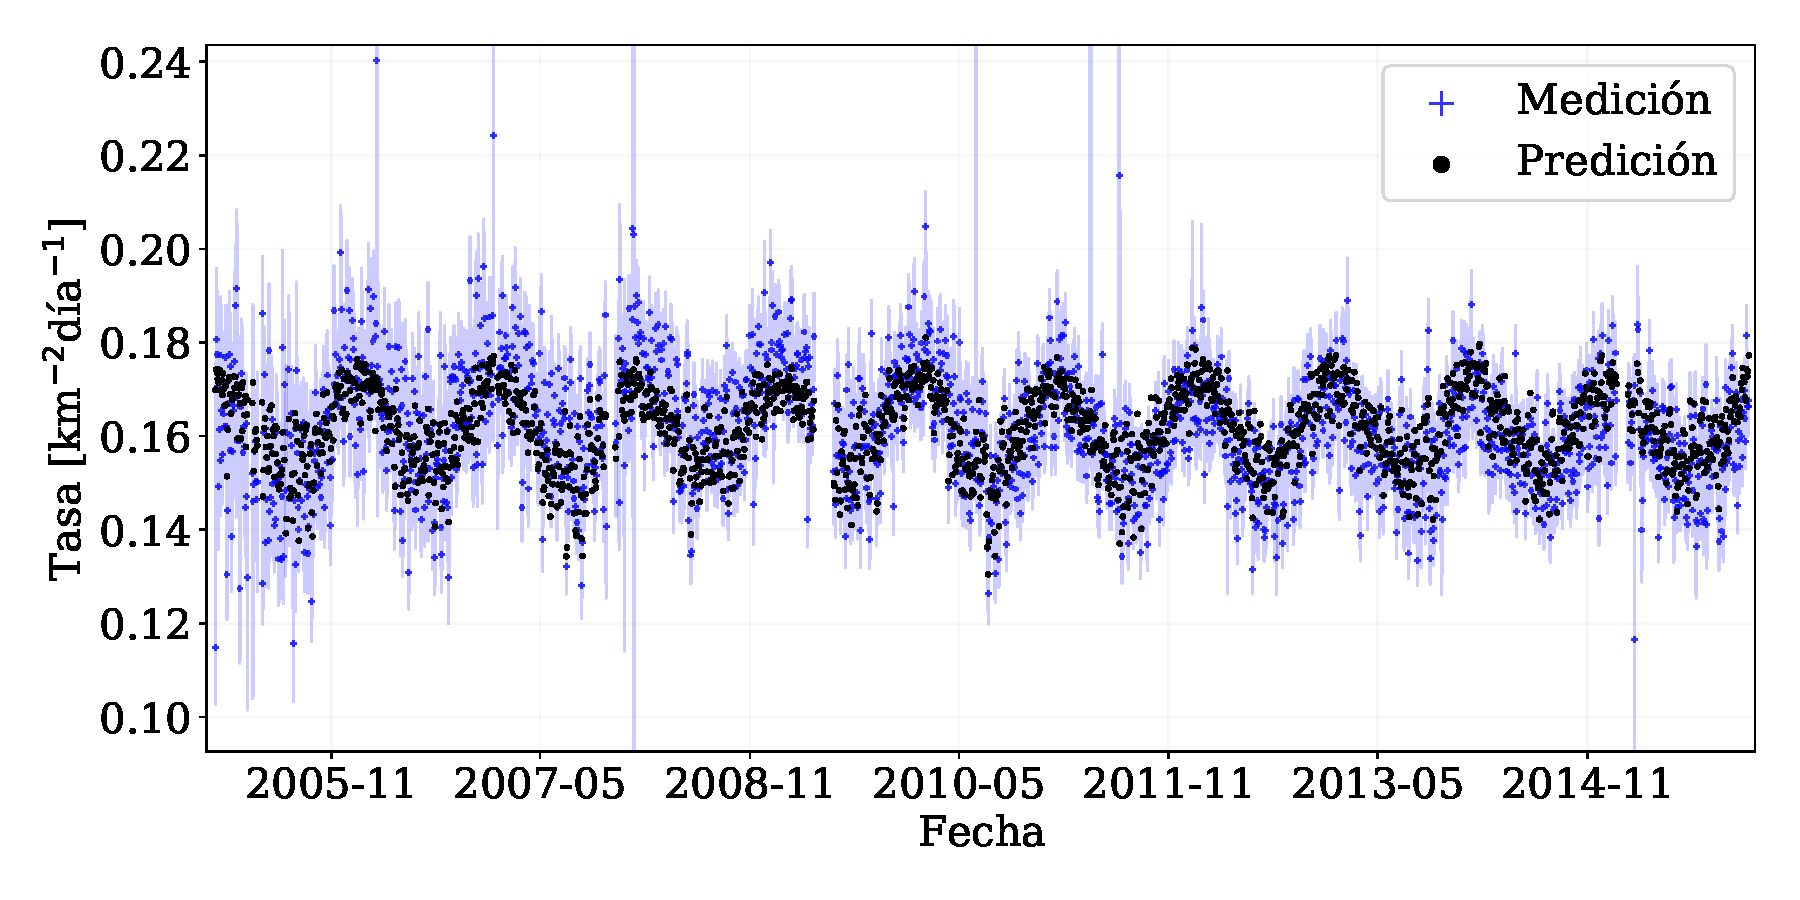
\includegraphics[width=\textwidth]{Graphs/rate_dayly/herald_old_above_1EeV_rate_day.pdf}
            \caption{Tasa eventos por día}\label{fig:rate_dayly_ICRC_2015}
            \end{subfigure}\\
            % \hspace{\fill}
            \begin{subfigure}[b]{0.875\textwidth}
            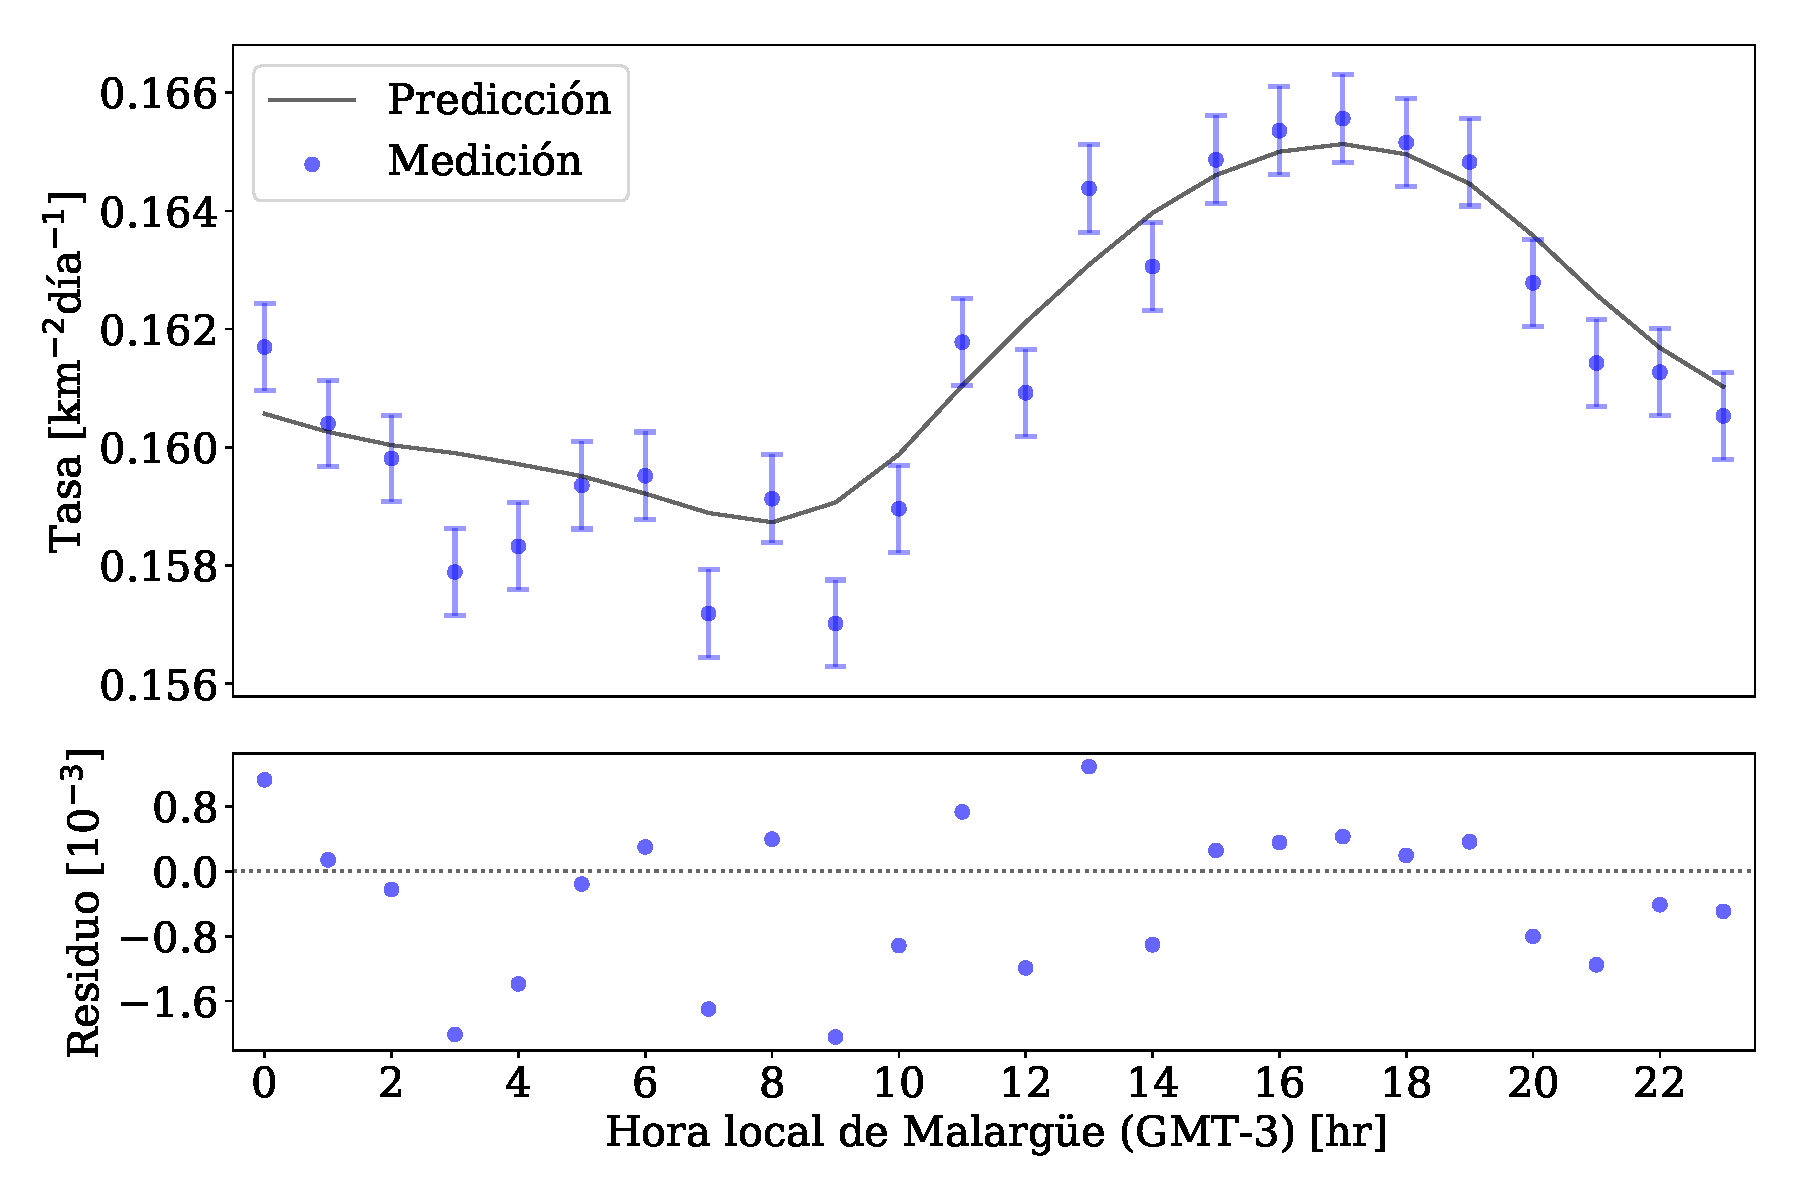
\includegraphics[width=\textwidth]{Graphs/rate_hour_of_the_day/1EeV_ICRC_2015_old_herald.pdf}
            \caption{Tasa de eventos promediada por hora del día }\label{fig:rate_hod_ICRC_2015}
            \end{subfigure}%
            \caption{Tasa de eventos por días comparadas con el ajuste entre los años 2005 hasta 2015. Los datos analizados fueron los presentados en la ICRC 2015 para energías mayores a $1\,$EeV donde se observa la modulación anual y diaria del clima. }\label{fig:rate_2015_05-15}
        \end{figure}


        Como se menciona en la sección \ref{seccion:sd_eff}, el detector alcanza su máxima eficiencia para energías mayores que 3\,EeV. A partir una energía de $2\,$EeV, los eventos tienen una mayor susceptibilidad al disparo de tres tanques, mínimo número necesario para la reconstrucción de un evento. Para el conjunto A, como se muestra en la Fig.\,\ref{fig:rate_2015_05-15_2EeV}, la modulación del clima aún es apreciable para una energía mayor a $2\,$EeV con una menor amplitud que para eventos de energía mayor a $1\,$EeV. 

        \begin{figure}[H]
            \centering
            \begin{subfigure}[b]{0.875\textwidth}
            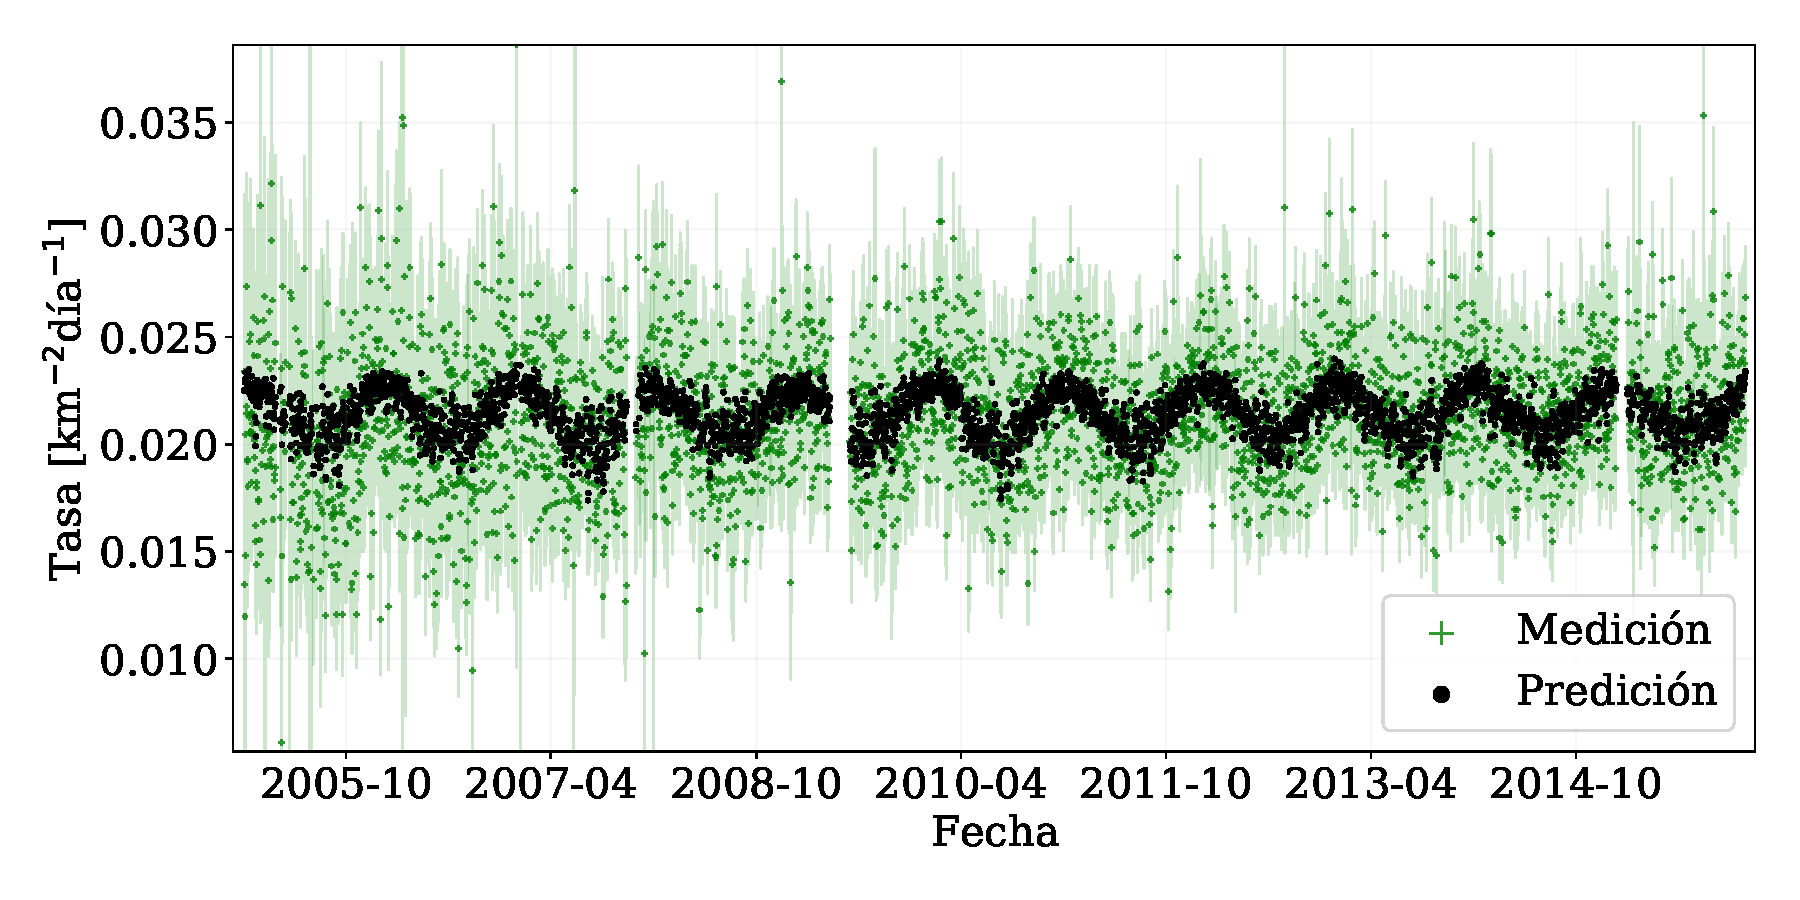
\includegraphics[width=\textwidth]{Graphs/rate_dayly/herald_old_above_2EeV_rate_day.pdf}
            \caption{Tasa eventos por día}\label{fig:rate_dayly_ICRC_2015_2EeV}
            \end{subfigure}\\
            % \hspace{\fill}
            \begin{subfigure}[b]{0.875\textwidth}
            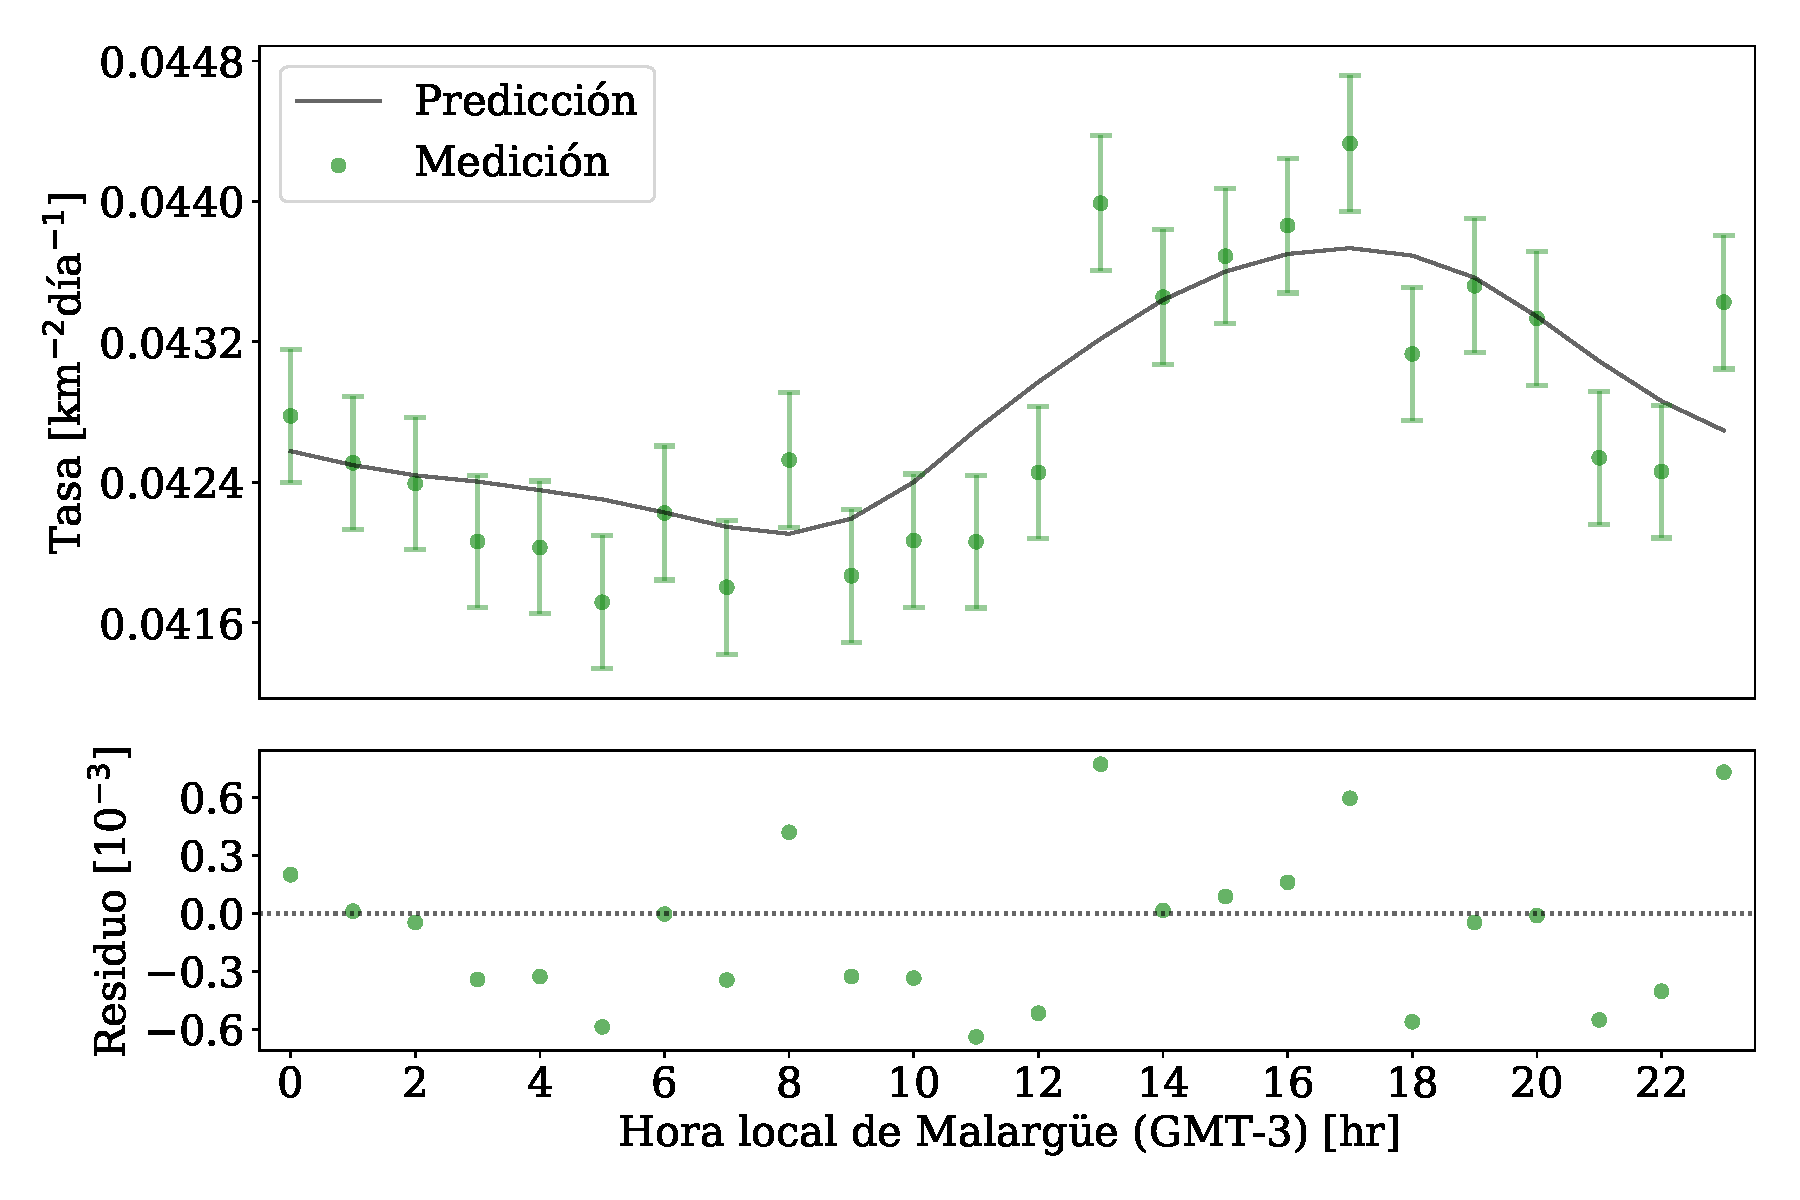
\includegraphics[width=\textwidth]{Graphs/rate_hour_of_the_day/herald_old_above_2EeV_hour_of_the_day.pdf}
            \caption{Tasa de eventos promediada por hora del día }\label{fig:rate_hod_ICRC_2015_2EeV}
            \end{subfigure}%
            \caption{Tasa de eventos por días comparadas con el ajuste entre los años 2005 hasta 2015. Los datos analizados son los presentados en la ICRC 2015 para energías mayores a $2\,$EeV. donde se observa la modulación anual y diaria del clima }\label{fig:rate_2015_05-15_2EeV}
        \end{figure}

%====|====|	Weather params
        \subsubsection{Ajuste de los parámetros del clima}
        En esta sección se estudia la dependencia de los parámetros del clima con el ángulo cenital. Clasificamos los eventos en distintos subconjuntos según el valor de $sin^2(\theta)$ para realizar un ajuste análogo al presentado en la Tabla \ref{tabla:parametros_ICRC_2015}. Se clasifica mediante este valor para obtener números de eventos similares para cada subconjunto. Estos ajustes son presentados en las Figs. \ref{fig:ap_2015}, \ref{fig:arho_2015} y \ref{fig:brho_2015}. Los mismos se comparan con los datos presentados en \cite{aab2017impact}, usados actualmente en la corrección de los datos del Observatorio Pierre Auger. Se observa que los ajustes hechos sobre el conjunto A son compatibles con los ajustes realizados en  el trabajo \cite{aab2017impact}. 
%====|====|====|	ap, arho, brho 2005-2015 vs JINST over 1 EeV
                \begin{figure}[H]
                    \centering
                    \begin{subfigure}[b]{0.75\textwidth}
                    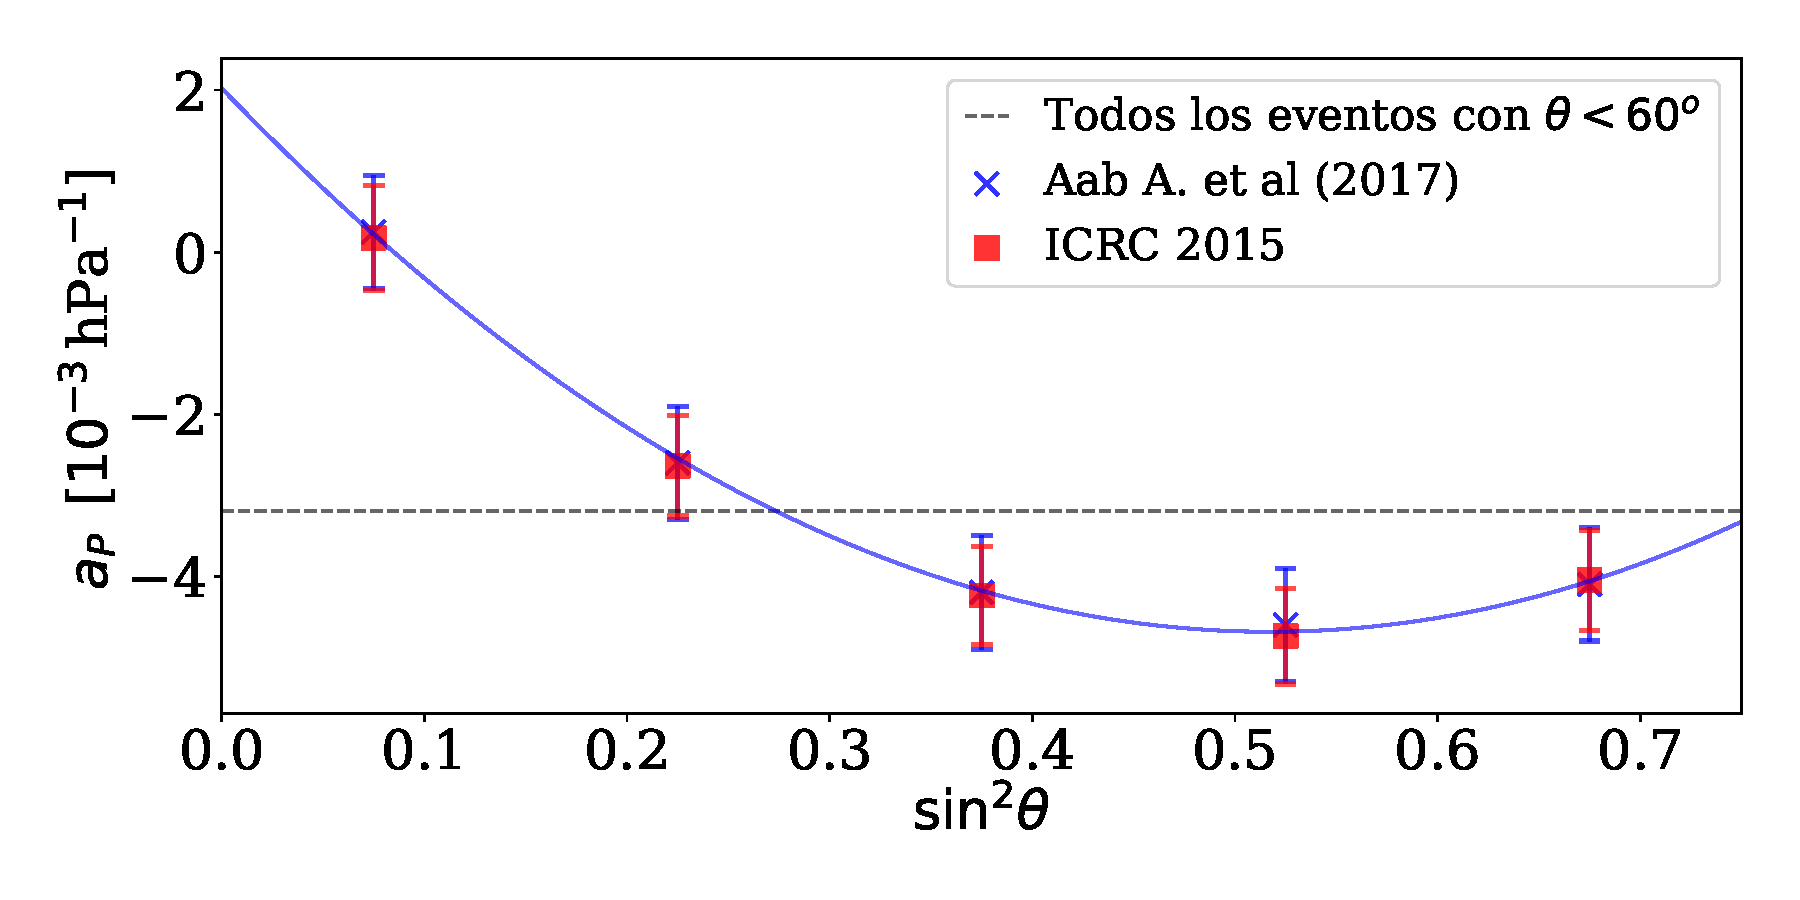
\includegraphics[width=\linewidth]{Graphs/params/ap_ICRC_2015_above_1EeV_v2.pdf}
                    \caption{Parámetro $a_P$ }
                    \label{fig:ap_2015}
                    \end{subfigure}\\
                    % \hspace{\fill}
                    \begin{subfigure}[b]{0.75\textwidth}
                    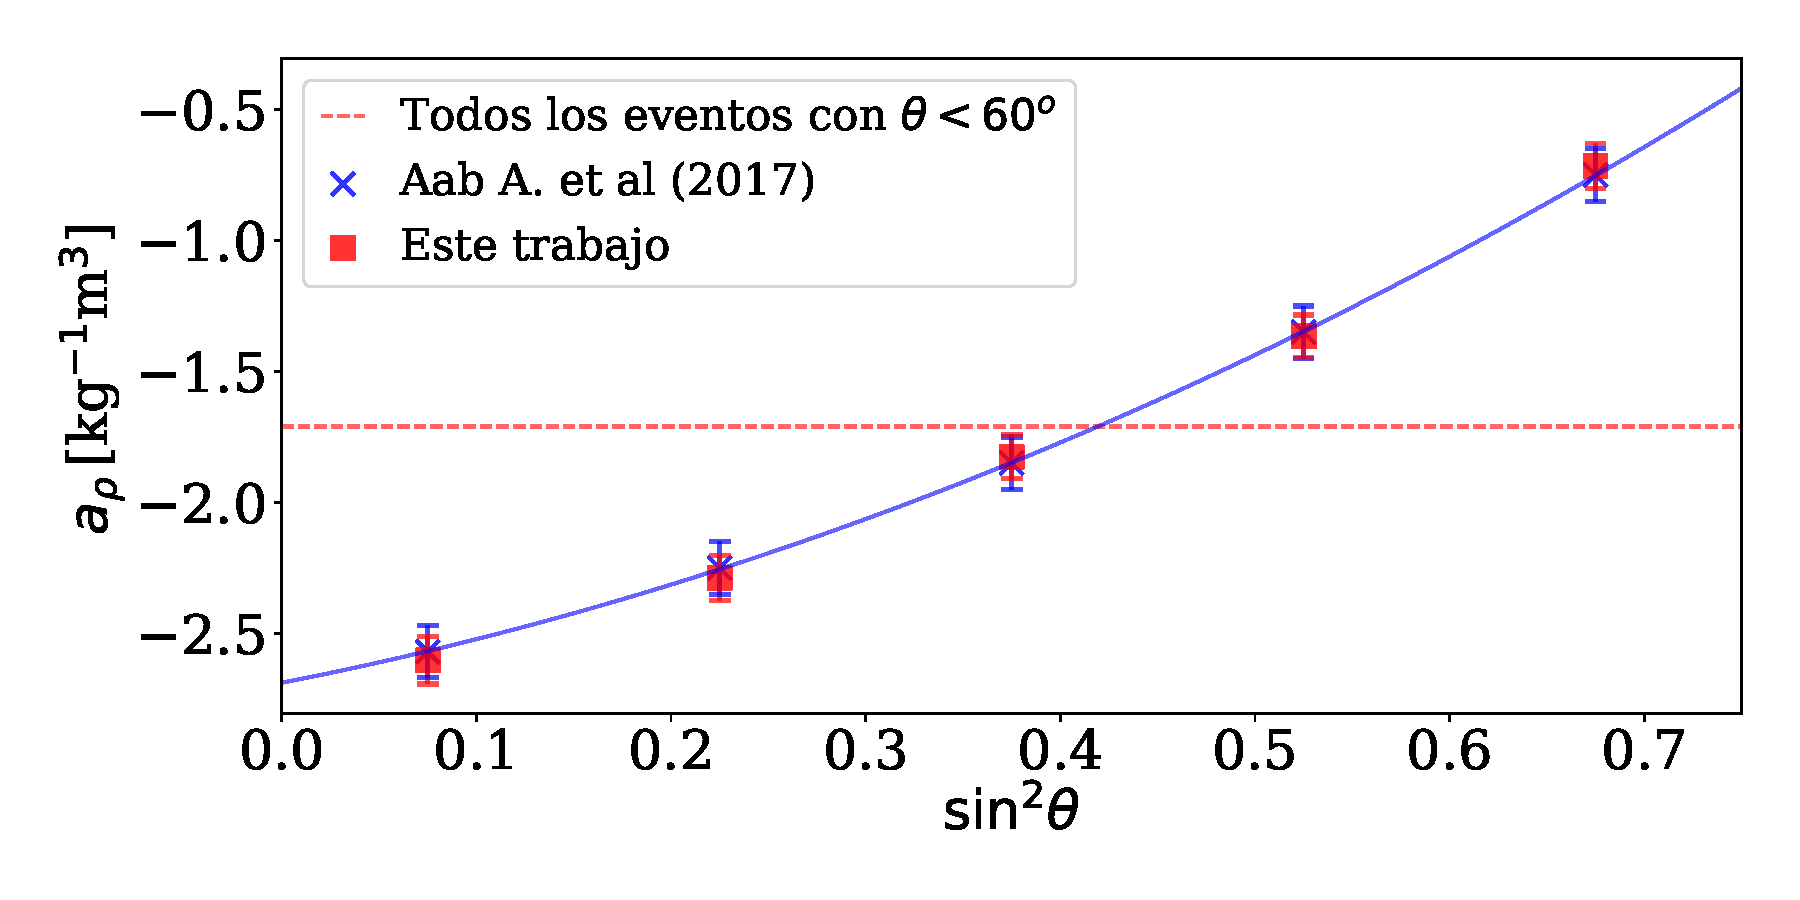
\includegraphics[width=\linewidth]{Graphs/params/arho_ICRC_2015_above_1EeV_v2.pdf}
                    \caption{Parámetro $a_{\rho}$ }
                    \label{fig:arho_2015}
                    \end{subfigure}\\
                    % \hspace{\fill}
                    \begin{subfigure}[b]{\textwidth}
                    \centering
                    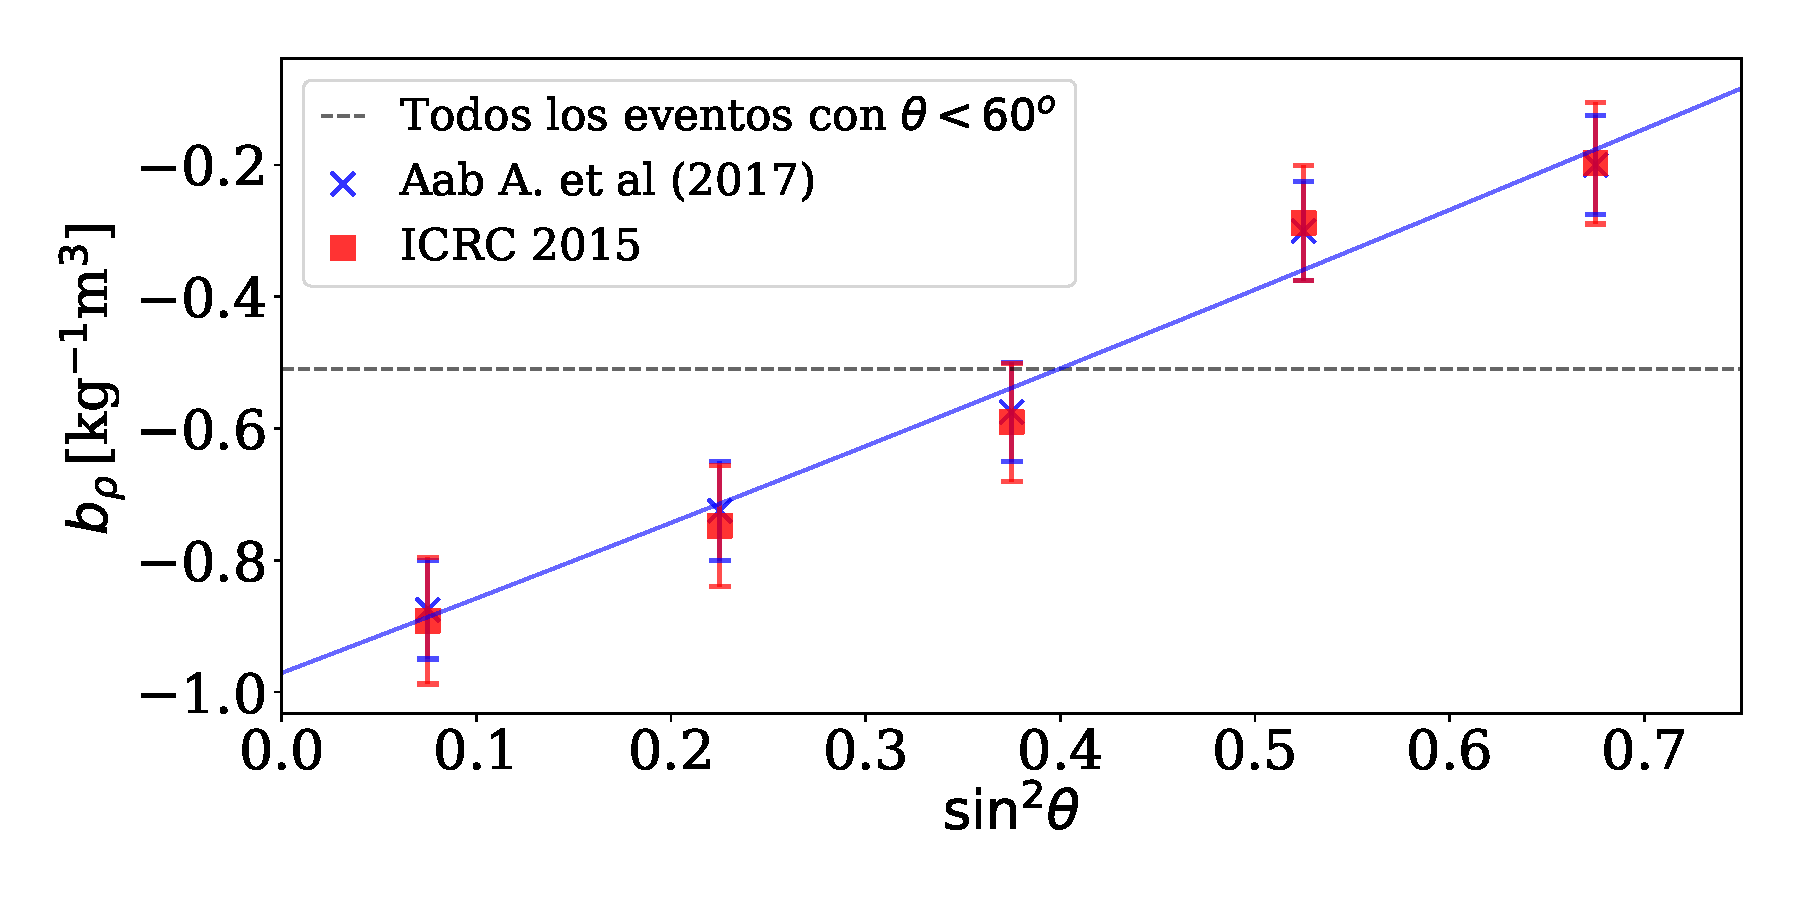
\includegraphics[width=0.75\linewidth]{Graphs/params/brho_ICRC_2015_above_1EeV_v2.pdf}
                    \caption{Parámetro  $b_{\rho}$	 }
                    \label{fig:brho_2015}
                    \end{subfigure}%
                    \caption{Parámetros de la modulación del clima considerando los datos de la ICRC 2015. Los mismos se comparan con los ajustes obtenidos por la Colaboración y con los ajustes obtenidos sin considerar la dependencia con $sin^2(\theta)$. }\label{fig:parameters_old}
                \end{figure}
%====|====|====| 	Tabla de c0, c1, c2
            En la Fig. \ref{fig:parameters_old} también se compara los ajustes obtenidos considerando los datos sin clasificar por $sin^2\theta$. Se observa que existe una dependencia con el ángulo cenital correspondiente al evento. Esta dependencia fue modelada mediante una función cuadrática dada en la Ec.\,\ref{eq:cuadratica}
            \begin{equation}
                f(x) = c_0 + c_1x + c_2x^2
                \label{eq:cuadratica}
            \end{equation}
            donde $x=sin^2\theta$.  En la Tabla\,\ref{tabla:cuadratica_ICRC_2015} se comparan los coeficientes obtenidos considerando la Ec.\,\ref{eq:cuadratica} con los mismos coeficiente obtenidos en el trabajo anterior \cite{aab2017impact}. 

        La dependencia con el ángulo cenital se debe a que para distintos ángulos de incidencia la lluvia interactúa con más o menos atmósfera. Los efectos de las condiciones climáticas afectan el desarrollo de la lluvia. Por ejemplo, el coeficiente de la presión  es negativo para $\sin^2(\theta)>0.3$ o $\theta>33^o$, lo que indica que si la presión sube la señal baja. Esto es una consecuencia de que la lluvia  está en un estado más avanzado de su desarrollo. Para ángulos cenitales cercanos a $60^o$, la componente electromagnética es suprimida por las interacciones en la atmósfera, por lo tanto el efecto de la presión disminuye. El resultado obtenido en la Fig.\,\ref{fig:ap_2015} es consistente con este fenómeno, dado que el valor de $a_P$ disminuye al aumentar el ángulo. 		En el caso de los coeficientes relacionados con la densidad, también se observa que los parámetros son negativos, dado que un aumento de la densidad disminuye $r_M$ y por lo tanto la extensión de la señal. Se observa también que los parámetros $a_\rho$ y $b_\rho$ tienen la misma tendencia con $\sin^2(\theta)$, además de que los coeficientes tienen una razón de aproximadamente $\nicefrac{1}{3}$, lo cual se esperaba por lo discutido en la sección \ref{seccion:fisica_clima}.
                \begin{table}[H]
                    \centering
                    \begin{tabular}{l|l|l|l}
                         Parámetros									& Coeficiente		& Este Trabajo			& \cite{aab2017impact}	\\ \hline \hline
                     \multirow{3}{*}{$a_P$ [hPa$^{-1}$]}  			&  $c_0$			& $( 2.00\pm 0.05)\times 10^{-3}$	& $( 2.1 \pm 0.9)\times 10^{-3} $	\\ \cline{2-4} %Done
                                                                    &  $c_1$			& $(-26.3 \pm 0.2)\times 10^{-3}$	& $(-26.0 \pm 0.6 )\times 10^{-3}$	\\ \cline{2-4} 
                                                                    &  $c_2$			& $( 25.7 \pm 0.2)\times 10^{-3}$	& $( 26.0 \pm 0.7 )\times 10^{-3}$	\\ \hline \hline% 
                    
                     \multirow{3}{*}{$a_\rho$ [kg$^{-1}$m$^3$]}  	&  $c_0$			& $-2.73   \pm 0.05$	& $ -2.7  \pm 0.1  $\\ \cline{2-4} 
                                                                    &  $c_1$			& $ 1.5    \pm 0.4 $	& $ 1.5   \pm 0.8  $\\ \cline{2-4} 
                                                                    &  $c_2$			& $ 2.1    \pm 0.7 $	& $ 2.2   \pm 1.0  $\\ \hline \hline%
                    
                    \multirow{3}{*}{$b_\rho$ [kg$^{-1}$m$^3$]} 		&  $c_0$			& $-1.0    \pm 0.1$		& $-1.0   \pm 0.1 $	\\ \cline{2-4} 
                                                                    &  $c_1$			& $ 1.2    \pm 0.6$		& $ 1.2   \pm 0.8  $	\\ \cline{2-4} 
                                                                    &  $c_2$			& $ 0.1    \pm 0.8$		& $ 0.0   \pm 1.1  $	\\ 
                    
                    \end{tabular}	
                    \caption{Tabla de los coeficientes obtenidos para el conjunto de datos de la ICRC 2015, comparados con los parámetros de la reconstrucción de los eventos del Observatorio.} \label{tabla:cuadratica_ICRC_2015}
                \end{table}

%==================================================================================
%==================================================================================
%==================================================================================
%==================================================================================


	%====|==> ICRC 2019
\subsection{Datos presentados en la ICRC 2019}\label{conjuntoB}

Este conjunto de datos contiene eventos de los tres años posteriores con respecto  a los datos del ICRC 2017. Posteriormente al trabajo \cite{aab2017impact}, la señal de S(1000) fue corregida por las condiciones climáticas en la reconstrucción oficial de eventos. Además el valor de S(1000) estimado para cada evento cambió entre estos dos conjuntos de datos, por parte de la reconstrucción oficial \cite{isabel}. Se realizó también una nueva calibración de la energía mediante eventos híbridos, como la mostrada en la Fig.\,\ref{fig:efd_s38} en el trabajo  \cite{tobepublished}. 

En el conjunto de datos de la ICRC 2019, se realizó los mismos cortes que para el conjunto de A de la sección anterior. En el periodo 2005-2015 de los datos de la ICRC 2019 con los cortes mencionados de energía mayor a $1\,$EeV para eventos verticales, la cantidad de eventos con energías mayores a $1\,$EeV subió de $1\,146\,470$ a  $1\,280\,918$ eventos. %Esto puede deberse a la corrección del clima de los eventos, donde aquellos eventos que estaban por debajo del corte de energía, tras la corrección pudieron estar por encima de este corte. 
Una posibilidad es que la nueva reconstrucción implementada sobre los datos del ICRC 2019, haya aumentado la cantidad de eventos por encima de $1\,$EeV, por eso la energía media bajó de $2.00\,$EeV a $1.91\,$EeV.  Las características de los datos en los rangos de tiempo relevantes se resumen en la Tabla\,\ref{tabla:caracteristicas_ICRC_2019}. 

%====|====|	Tabla de eventos exposure
   \begin{table}[H]
       \centering
       \begin{tabular}{r|c|c|}
    %    {Tiempo }           & {01/01/2005-31/12/2015}   & {01/01/2005-31/12/2018 }\\ \hline 
    \cline{2-3}
                              & \multicolumn{2}{c|}{ICRC 2019} \\ \cline{2-3}
         Inicio:              & 01/01/2005      & 01/01/2005\\
         Fin:                 & 31/12/2015      & 31/12/2018\\  
         Número de eventos:   &  $1\,280\,918$     			    &  1635045     		        \\ 
         Energía media:       &  1.91				        &	1.92				        \\ 
         Corte en energía:    &  $>1$ EeV       		 	    &  $>1$  EeV       		 \\ 
         Corte en ángulo cenital:	&  $\theta<60^o$ 				    & $\theta < 60^o$\\ \cline{2-3}
       \end{tabular}
       \caption{Características de los datos de la ICRC 2019 utilizados para los ajustes de esta sección.} \label{tabla:caracteristicas_ICRC_2019}
   \end{table}

   En la Fig.\,\ref{fig:rate_new_18} se muestran las tasas de eventos por día para energía mayores a $1\,$EeV y $2\,$EeV, con la energía corregida por los efectos climáticos según la reconstrucción oficial \cite{data}.  Comparemos las tasas de eventos por hora del día de los eventos, por encima de $1\,$EeV y $2\,$EeV con las tasas para el conjunto  A. Por encima de $1\,$EeV, se aprecia un remanente de la modulación del clima diaria comparado con la tasa para $2\,$EeV. Esto se debe a que el arreglo principal tiene eficiencia completas para energías mayores a $3\,$EeV, comentado anteriormente. Por encima de 2\,EeV, la modulación en la tasa ya no es apreciable. 


   Existe una modulación remanente en la tasa de eventos con energía mayor a 1 EeV como se aprecia en la Fig.\,\ref{fig:rate_new_18} y \ref{fig:rate_new_18_2EeV}. Esto se debe que la señal es mayor que la esperada como consecuencia de las condiciones atmosféricas en el momento del evento, por lo tanto la eficiencia del disparo ante este evento también es mayor. De esta forma la eficiencia tiene una dependencia con las condiciones atmosféricas.
%====|====|	2005-2019	rate day over 1 EeV
%====|====|	2005-2019	rate hour of the day	1 EeV
   \begin{figure}[H]
       \centering
      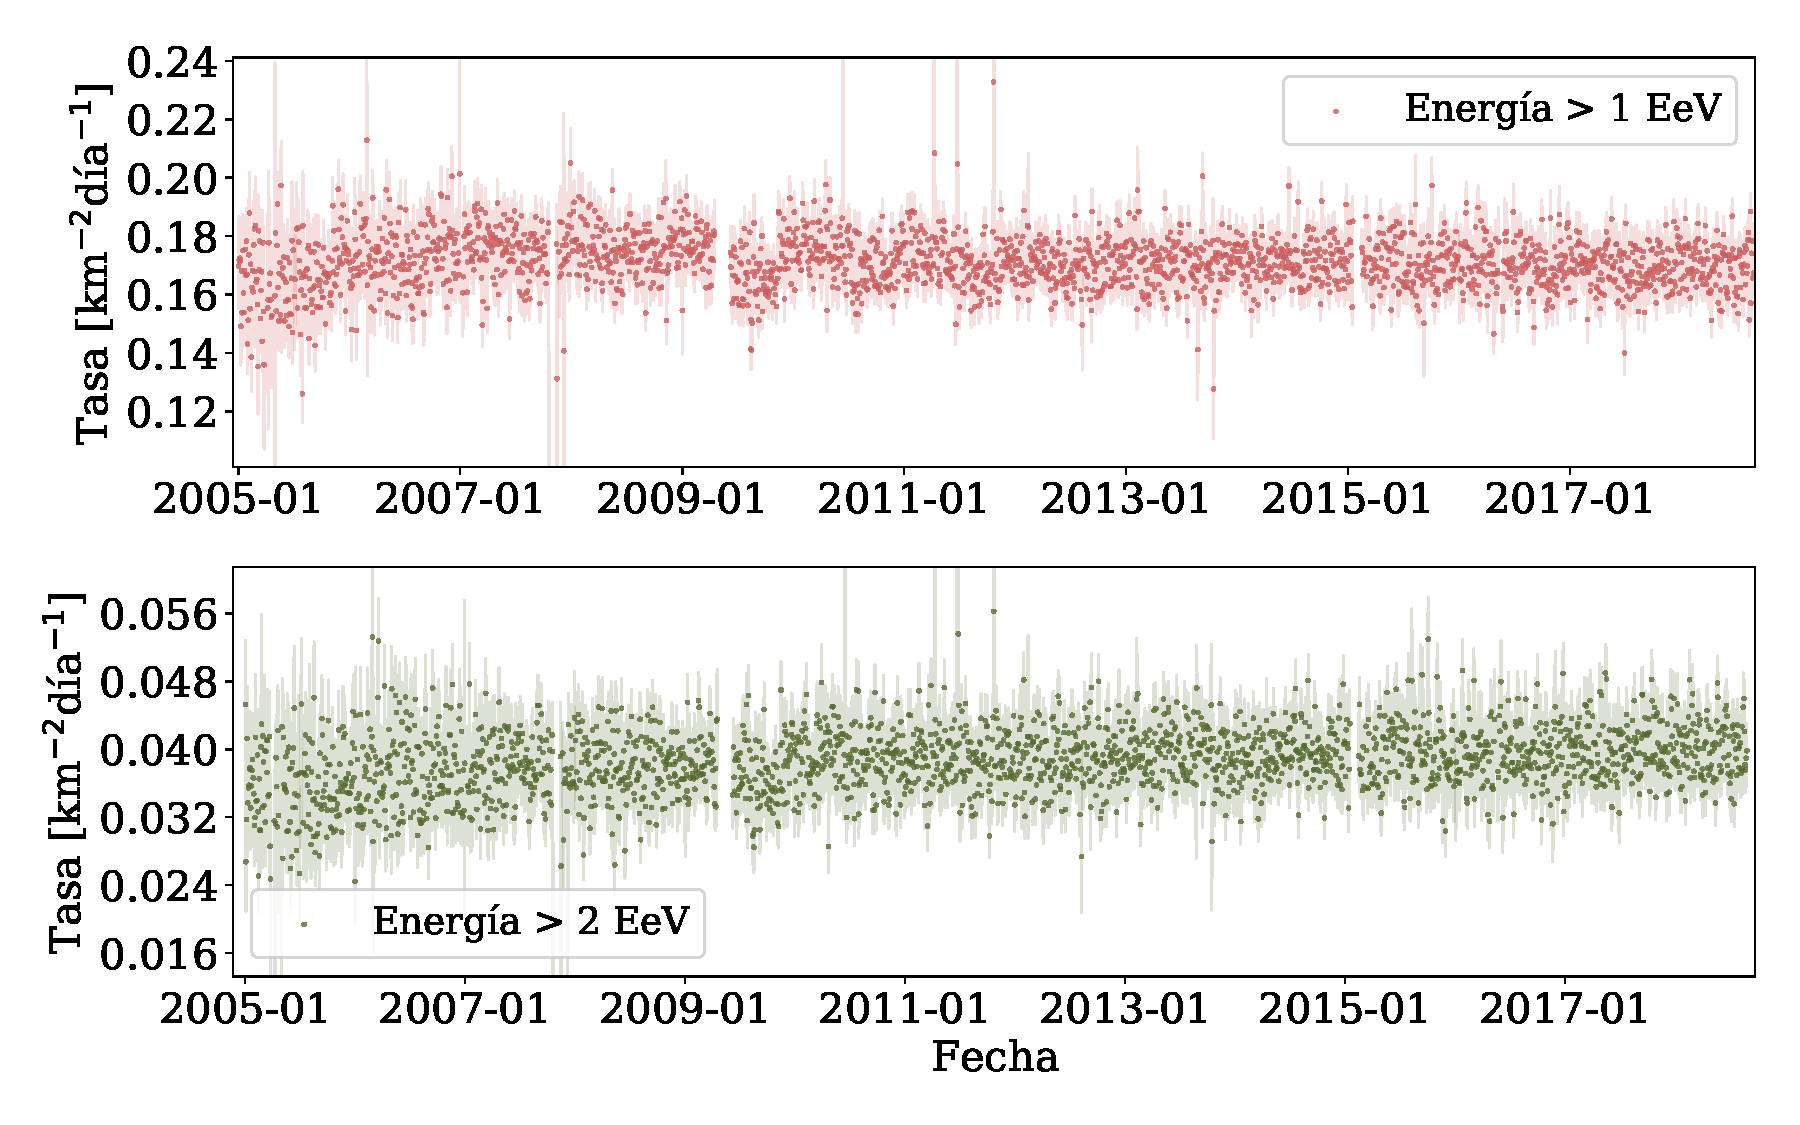
\includegraphics[width=0.8\textwidth]{Graphs/rate_dayly/herald_above_1EeV_2EeV_rate_day.pdf}
       \caption{Tasa de eventos promedio por cada día desde inicios del 2005 hasta inicios del 2018 del conjunto de datos presentado en la ICRC 2019. Se muestran las tasas para dos cortes en energía, mayor a $1\,$EeV y mayor a $2\,$EeV}\label{fig:rate_new_18}
   \end{figure}



   \begin{figure}[H]
       \centering
      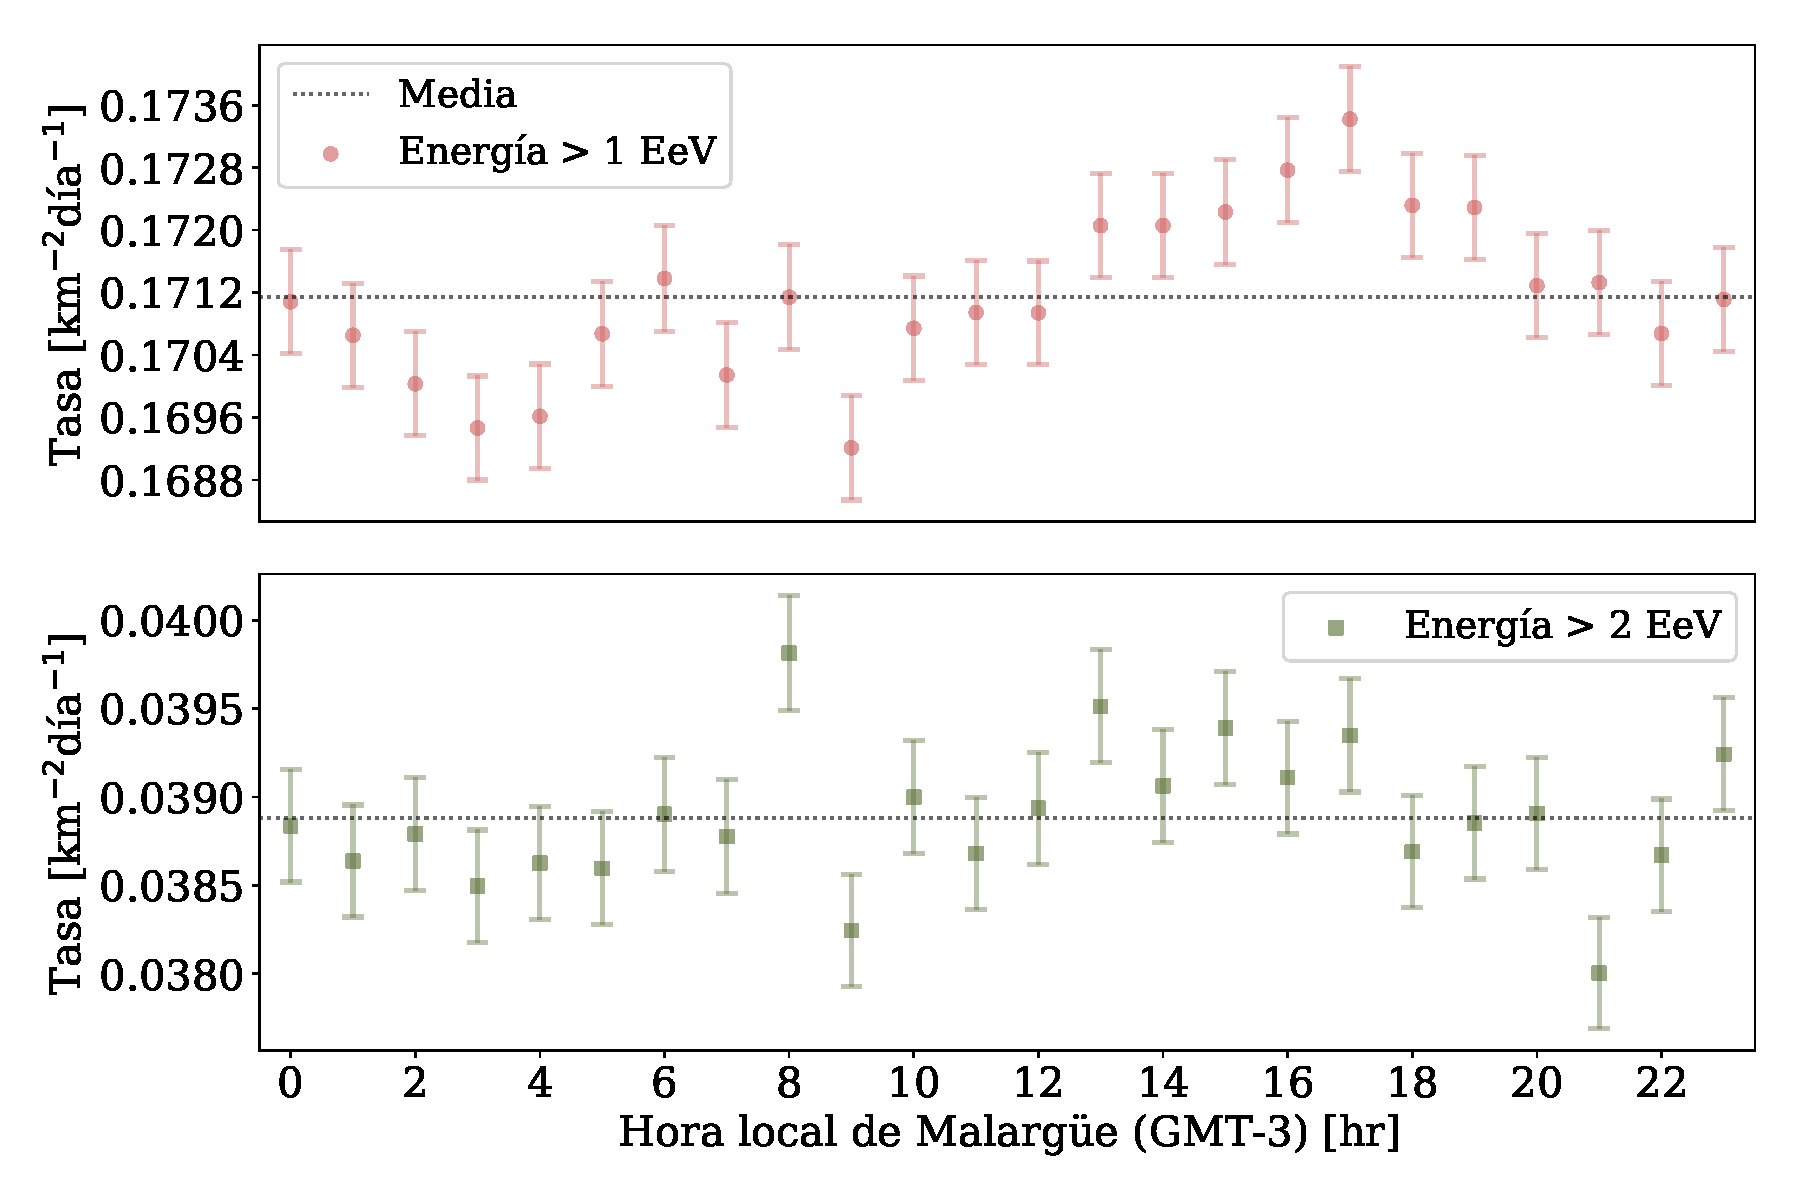
\includegraphics[width=0.8\textwidth]{Graphs/rate_hour_of_the_day/herald_above_1EeV_and_2EeV_hour_of_the_day.pdf}
       \caption{Tasas de eventos  por hora del día por unidad de área desde inicios del 2005 hasta inicios del 2018 del conjunto de datos presentado en la ICRC 2019.  Se muestran las tasas para dos cortes en energía, mayor a $1\,$EeV y mayor a $2\,$EeV}\label{fig:rate_new_18_2EeV}
   \end{figure}


%====|==>ICRC 2019 S$_{38}$-Sin Corrección
\subsection{Datos presentados en la ICRC 2019 usando $S_{38}$ sin corregir por el clima} \label{sin_corregir_s38}


Además de tener más estadística de los eventos registrados, durante el periodo 2016-2018 también se recabaron datos sobre el clima en el observatorio. En la modulación del clima estudiada con el conjunto A, se  realiza un corte de la energía sin corregir. En esta sección se realiza el análisis de la modulación mediante un  corte sobre la señal medida por el arreglo principal. En el conjunto de datos de la ICRC 2019, es posible acceder al valor de S(1000) sin corregir por el trabajo \cite{aab2017impact}, por lo que uno puede obtener el valor de S$_{38}$ sin corregir mediante la expresión
\begin{equation}
S_{38} = \frac{S(1000)}{S(1000)_w}S_{38,w}
\label{eq:s38_w}
\end{equation}
donde las variables $S(1000)_w$ y $S_{38,w}$ indican los valores corregidos por clima. Estas variables están listadas en el conjunto de datos presentado en la ICRC 2019. 

Dado que los trabajos anteriores se basaron en la energía para hacer el corte de los eventos, se realizó el corte con la señal de $S_{38}\ge 5.37\,$VEM correspondiente a 1\,EeV aproximadamente. Las características de este conjunto de datos están resumidos en la Tabla\,\ref{tabla:caracteristicas_ICRC_2019_S38}.
%====|====|	Tabla de eventos exposure
   \begin{table}[H]
       \centering
       \begin{tabular}{r|c|c|}
    %    {Tiempo}                & {01/01/2005-31/12/2015}   & {01/01/2005-31/12/2018 }\\ \hline
    \cline{2-3}
                              & \multicolumn{2}{c|}{ICRC 2019} \\ \cline{2-3}
 
       Inicio:                 & 01/01/2005                 &  01/01/2005 \\
       Fin:                    & 31/12/2015                 &   31/12/2018 \\
       Número de eventos:       &   $1\,267\,265$     	    &  $1\,618\,717$     		\\ 
       Energía media:           &  1.89        		 	    &  1.90        		\\  
       Corte en S$_{38}$: 	   &  $>5.37$\,VEM   		 	    &  $>5.37$\,VEM       	\\  
       Corte en ángulo cenital: &  $\theta<60^o$ 			 	 & $\theta<60^o$\\ \cline{2-3}
       \end{tabular}
       \caption{Características de los datos de la ICRC 2019 con el corte en la señal de S$_{38}$ utilizados para los ajustes de esta sección.} \label{tabla:caracteristicas_ICRC_2019_S38}
   \end{table}
   
%====|====| Tabla del fit
   Con estos eventos, se realizó un  ajuste de los parámetros del clima para todos los ángulos cenitales de la tasa de eventos por hora, así se obtienen los coeficientes promediados por ángulo cenital. Estos parámetros son presentados en la Tabla\,\ref{tabla:parametros_ICRC_2019_S38}. Se observa que para ambos periodos estudiados los parámetros obtenidos son compatibles entre sí, además de ser compatibles con los resultados obtenidos para el periodo 2005-2015 de los datos de la ICRC 2017 y los parámetros de \cite{aab2017impact} presentados en la Tabla\,\ref{tabla:parametros_ICRC_2017}.

   \begin{table}[H]
       \centering
       \begin{tabular}{c|c|c}
       {Parámetro}                 & {2005-2015}    		        & {2005-2018}    \\ \hline \hline
       $a_P$ [hPa$^{-1}$]          & $ (-3.3\pm 0.3)\times 10^{-3}$& $(-3.2\pm 0.2)\times 10^{-3}$  \\ \hline
       $a_\rho$ [kg$^{-1}$m$^3$]   & $ -1.75\pm 0.04$            	& $ -1.71\pm 0.03$       \\ \hline
       $b_\rho$ [kg$^{-1}$m$^3$]   & $ -0.51\pm 0.04$             	& $ -0.52\pm 0.03$       \\ \hline
       $\chi^2_\nu$                & $1.00616$                     & $1.01819$              \\   
       \end{tabular} 
       \caption{Parámetros del clima obtenidos para todos los ángulos cenitales para los dos rangos de tiempo estudiados de los datos de la ICRC 2019 con el corte en la señal de S$_{38}$.} \label{tabla:parametros_ICRC_2019_S38}
   \end{table}
   
   Calculando la tasa de eventos esperado con los parámetros de la Tabla\,\ref{tabla:parametros_ICRC_2019_S38}, esta se comparan con la tasa experimental medida con el arreglo principal, que se muestra en la Fig. \ref{fig:rate_new_18_S38} para el rango de tiempo 2005-2018. En estos gráficos se observa que la modulación del clima tiene las mismas características que las observadas en la sección \ref{icrc2015} salvo un aumento en la tasa media de eventos.

   \begin{figure}[H]
    \centering
       \begin{subfigure}[b]{0.85\textwidth}
       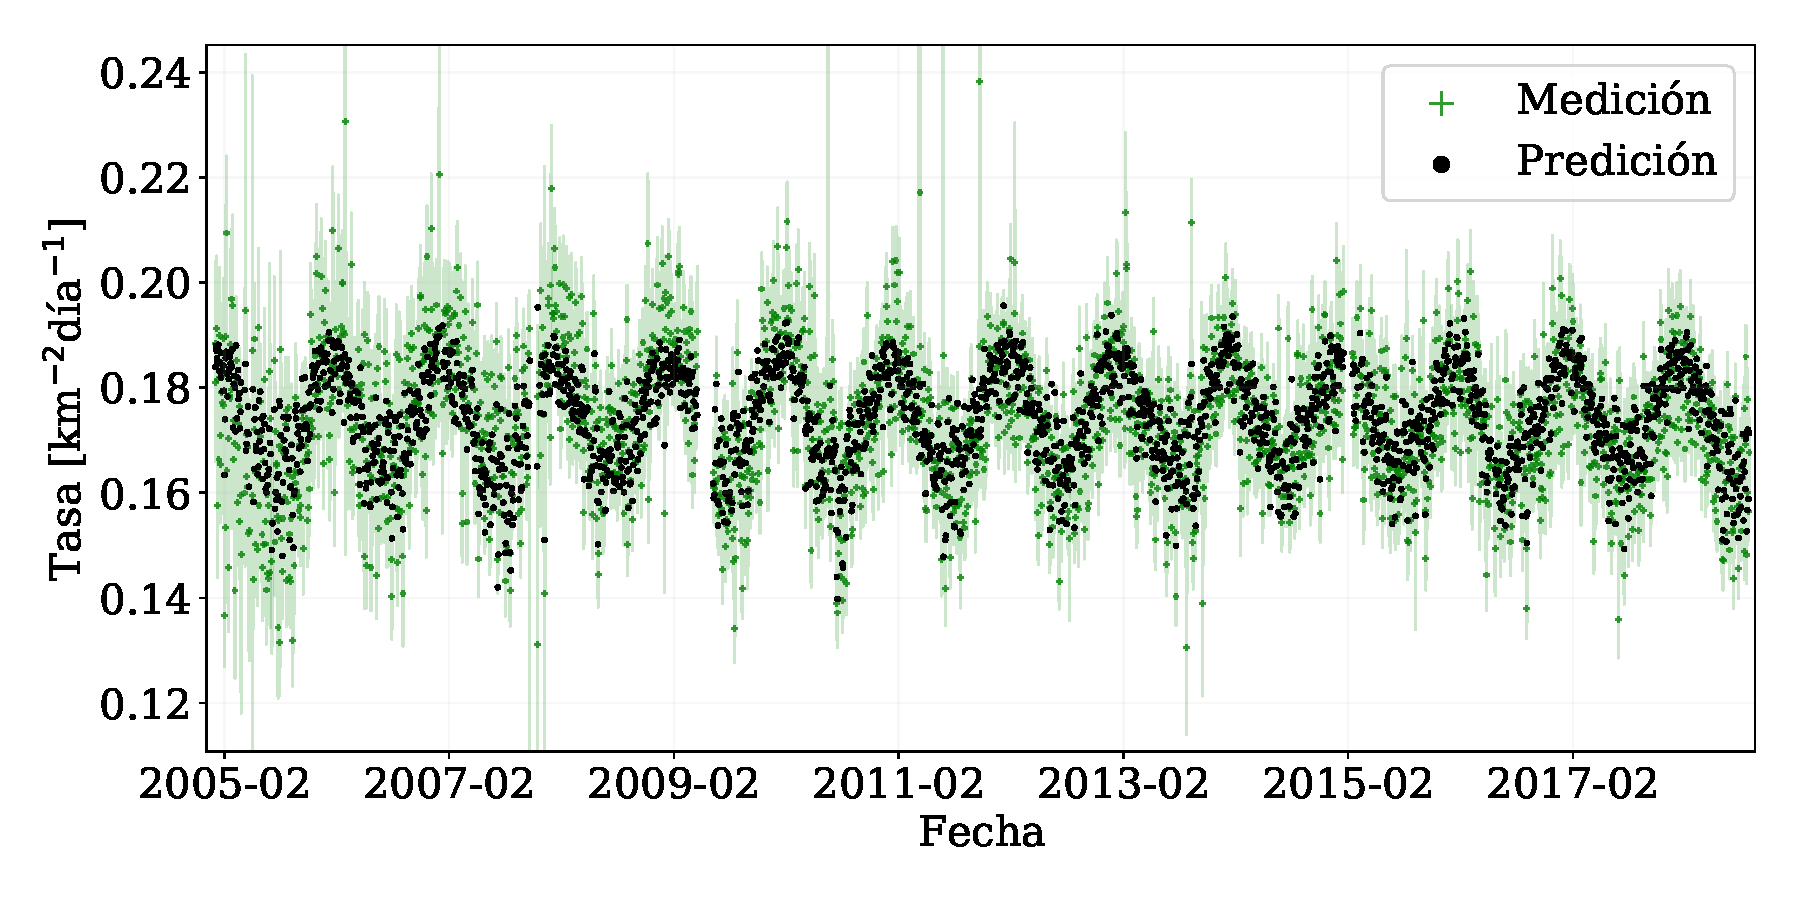
\includegraphics[width=\textwidth]{Graphs/rate_dayly/0EeV_ICRC_2019_S38_05_18.pdf}
       \caption{Tasa eventos por cada día por unidad de área}
       \label{fig:rate_day_ICRC_19_S38_05_18}
       \end{subfigure}\\%
    %    \hspace{\fill}
       \begin{subfigure}[b]{0.85\textwidth}
       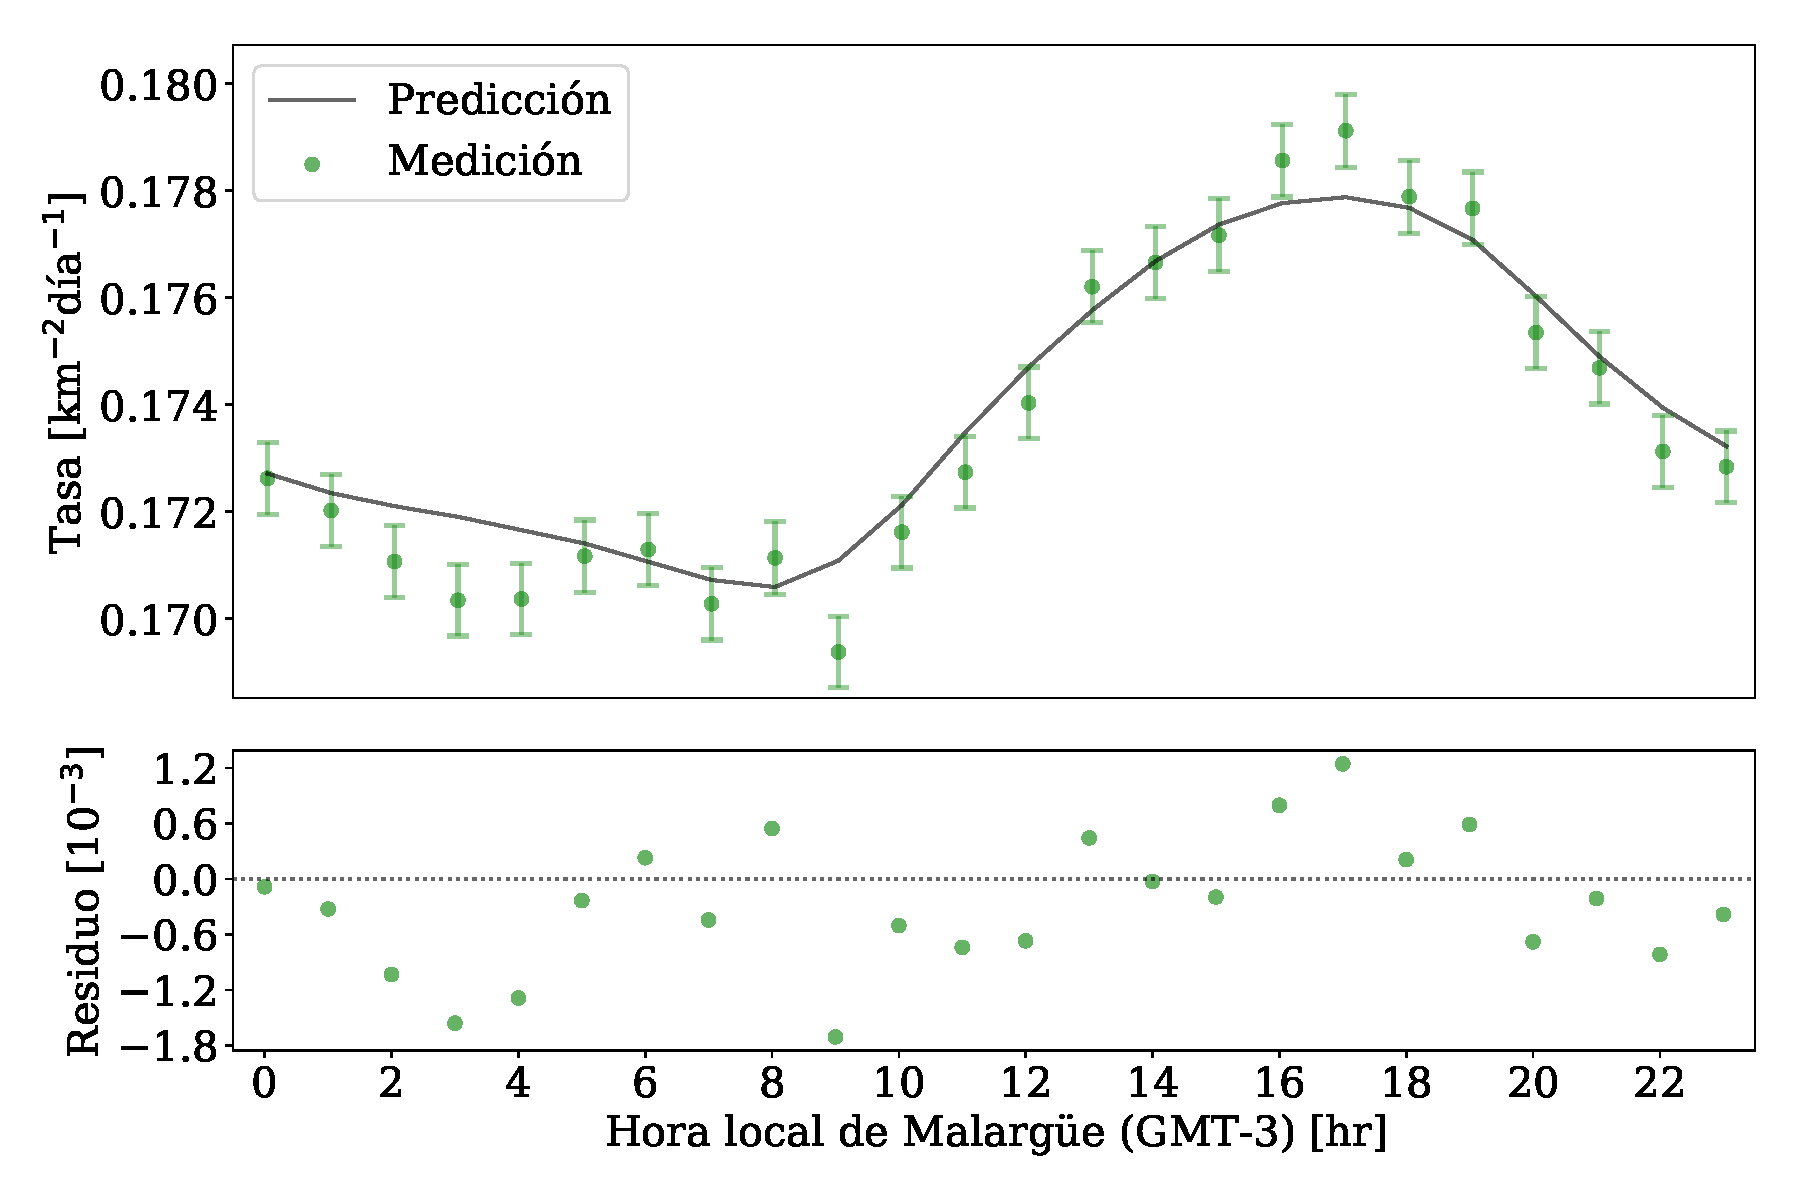
\includegraphics[width=\textwidth]{Graphs/rate_hour_of_the_day/S38_above_0EeV_hour_of_the_day.pdf}
       \caption{Tasa de eventos promedio por hora del día}
       \label{fig:rate_2015_ICRC_19_S38_05_18}
       \end{subfigure}%
       \caption{Tasa de eventos desde inicios del 2005 hasta inicios del 2018 de los datos de la ICRC 2019 con el corte en la señal de S$_{38}$. La predicción es obtenida por los parámetros calculados en este trabajo.}\label{fig:rate_new_18_S38}
   \end{figure}

%====|====|	Weather params
\subsubsection{Ajuste de los parámetros del clima}

En esta sección se clasificó los eventos mediante el valor de $sin^2\theta$ y se realizó el ajuste para obtener los parámetros del clima. Este ajuste se realizó en el periodo 2005-2018. Los valores obtenidos se resumen en la Tabla\,\ref{tabla:cuadratica_ICRC_2019_S38} y se  observan en la Fig.\,\ref{fig:parameters_new_S38}. Comparando estos resultados con los resultados de \cite{aab2017impact}, los eventos mediante el valor S$_{38}$  conservan la tendencia con $sin^2\theta$ que se observa en los datos de la ICRC 2017 en la Fig.\,\ref{fig:parameters_old}. Además los parámetros obtenidos mediante el corte por S$_{38}$ son comparables con los resultados obtenidos para el conjunto de datos de la ICRC 2017. Por lo que puede decirse que la modulación del clima es apreciable  hasta el día de hoy con una amplitud comparable al año 2015.

%====|====|====| ap, arho, brho 2005-2015  2005-2019 vs JINST over 1 EeV
       \begin{figure}[H]
        \centering
           \begin{subfigure}[b]{0.73\textwidth}
           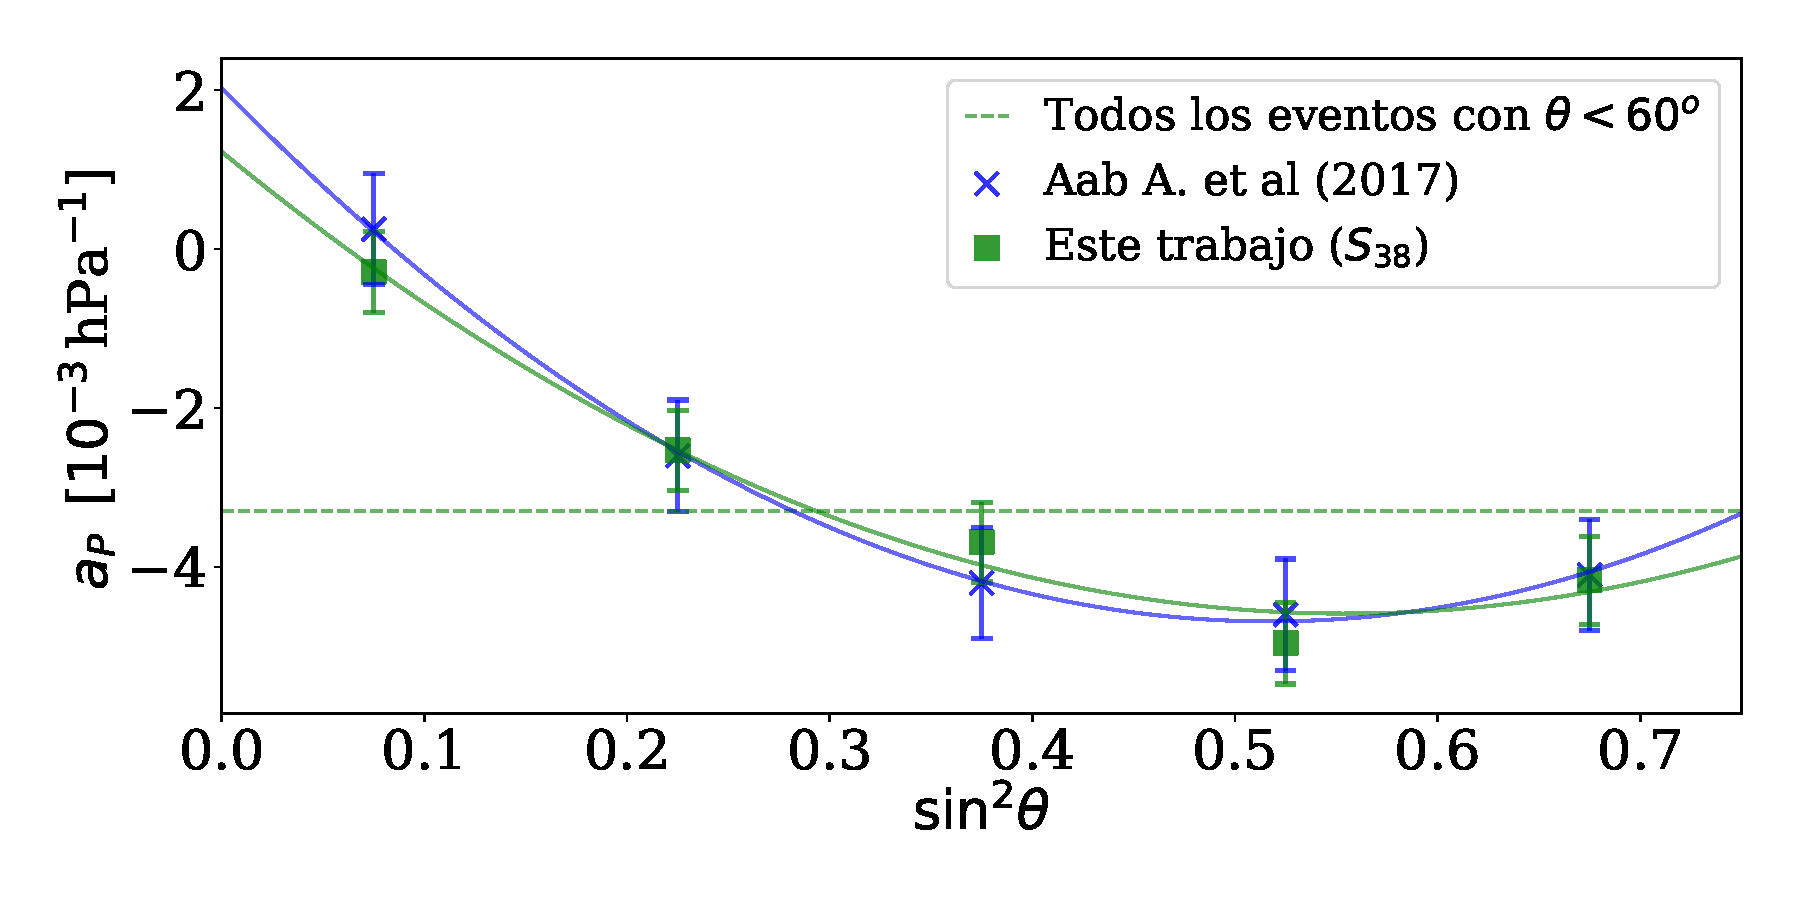
\includegraphics[width=\linewidth]{Graphs/params/ap_ICRC_2019_S38_above_0EeV.pdf}
           \caption{Parámetro $a_P$ }
           \label{fig:ap_2019_S38}
           \end{subfigure}\\%
        %    \hspace{\fill}
           \begin{subfigure}[b]{0.73\textwidth}
           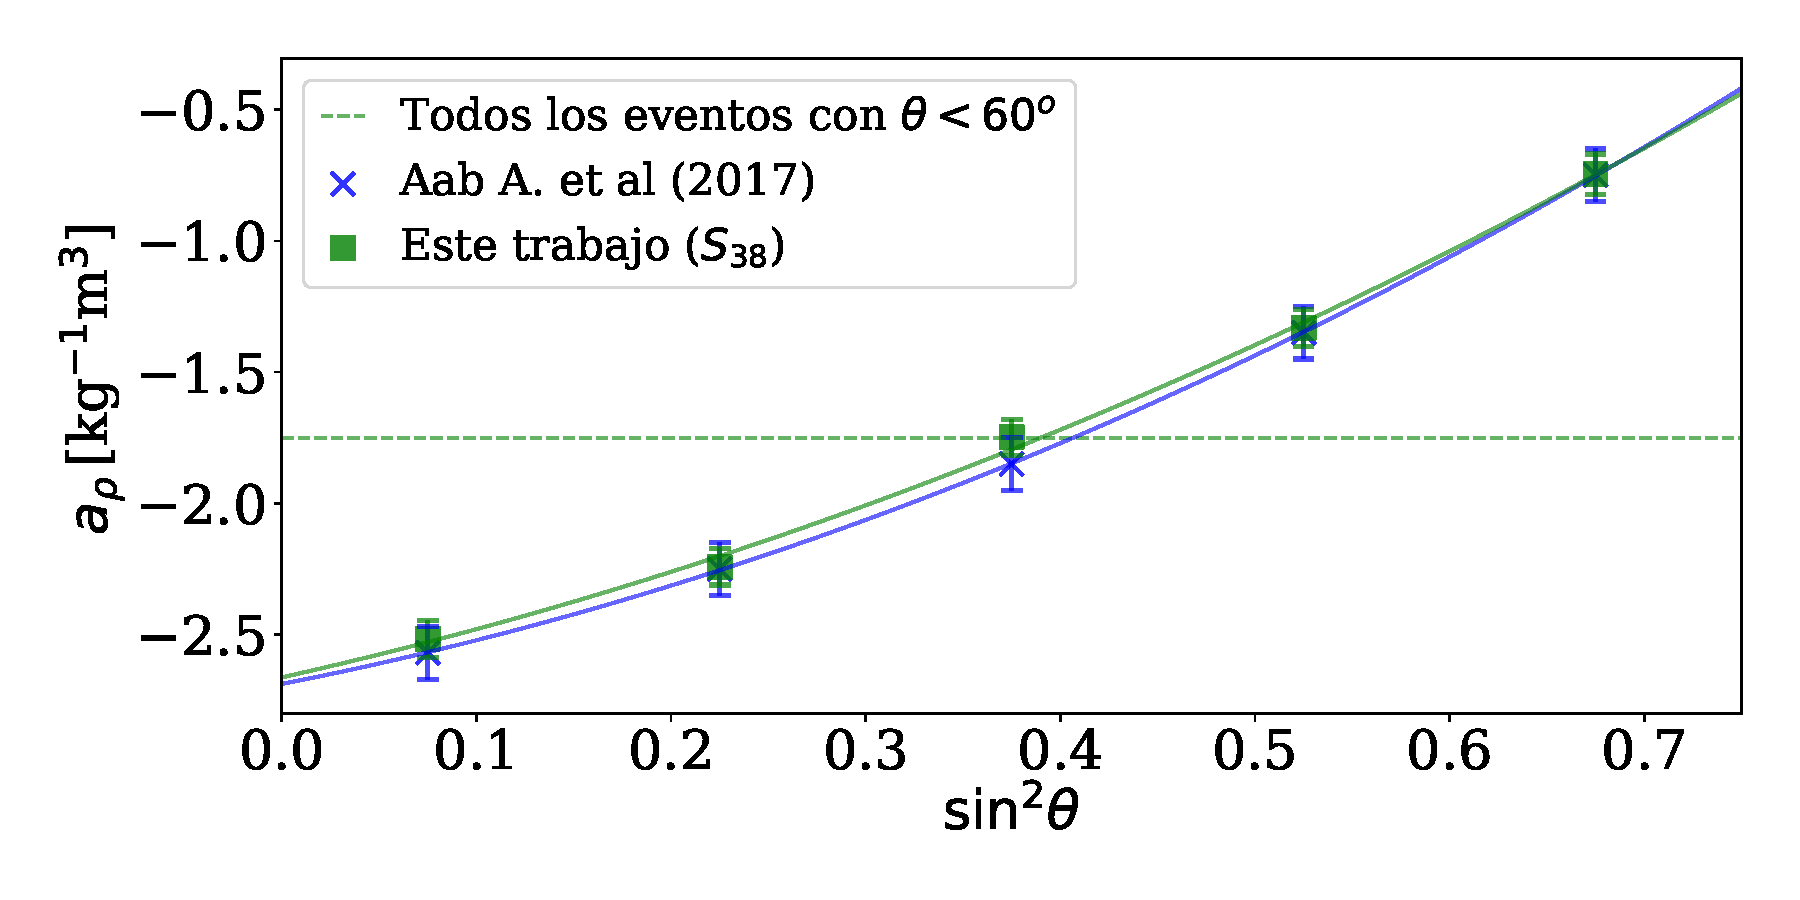
\includegraphics[width=\linewidth]{Graphs/params/arho_ICRC_2019_S38_above_0EeV.pdf}
           \caption{Parámetro $a_{\rho}$ }
           \label{fig:arho_2019_S38}
           \end{subfigure}\\%
        %    \hspace{\fill}
           \begin{subfigure}[b]{\textwidth}
           \centering
           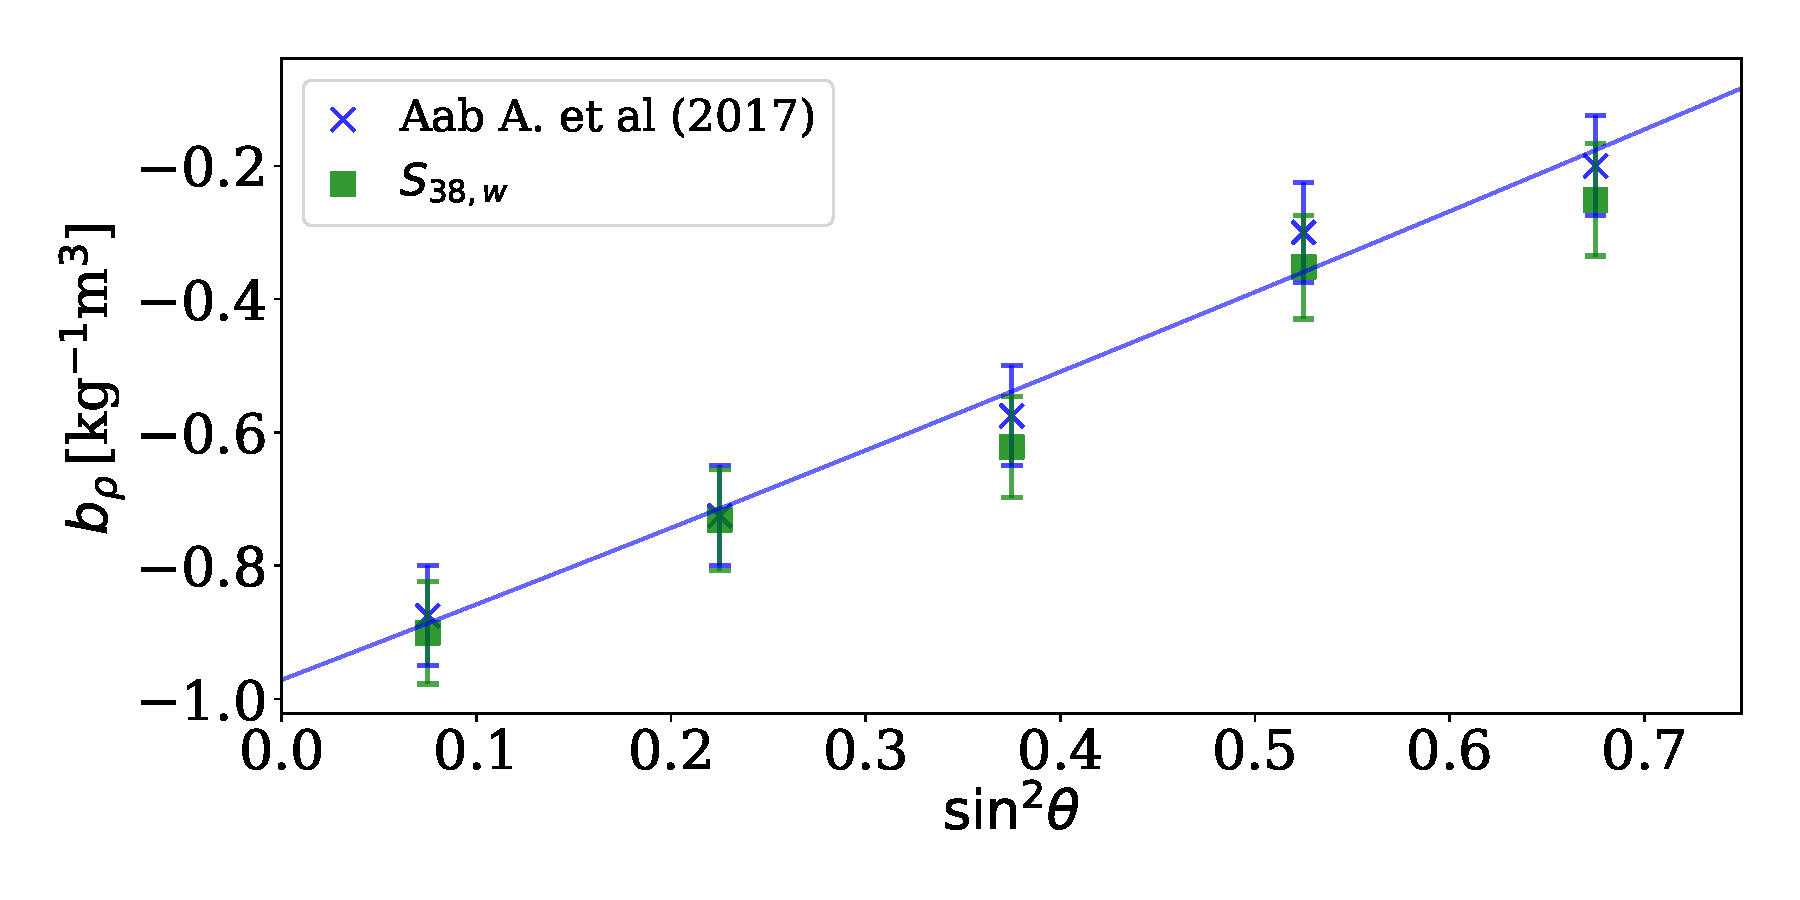
\includegraphics[width=0.73\linewidth]{Graphs/params/brho_ICRC_2019_S38_above_0EeV.pdf}
           \caption{Parámetro  $b_{\rho}$	 }
           \label{fig:brho_2019_S38}
           \end{subfigure}%
           \caption{Parámetros de la modulación del clima considerando los datos sin corregir con el clima y la reconstrucción anterior.}\label{fig:parameters_new_S38}
       \end{figure}
%====|====|====| Tabla de c0, c1, c2
           \begin{table}[H]
               \centering
               \begin{tabular}{l|l|l|l}
                {Parámetros}						        & {Coeficiente}	    & {Este Trabajo} & Reportado por { \cite{aab2017impact}}	\\ \hline \hline
                \multirow{3}{*}{$a_P$ [hPa$^{-1}$]}  		&  $c_0$				& $ (0.12\pm0.05)\times 10^{-3}$	    & $(2.1 \pm 0.09)\times 10^{-3} $	\\ \cline{2-4} %Done
                                                           &  $c_1$				& $ (-2.0\pm0.3)\times 10^{-3}$		& $(-2.6  \pm 0.6)\times 10^{-3} $	\\ \cline{2-4} 
                                                           &  $c_2$				& $ (1.9\pm0.4)\times 10^{-3}$		& $(2.6   \pm 0.7)\times 10^{-3} $	\\ \hline \hline% 
               
                \multirow{3}{*}{$a_\rho$ [kg$^{-1}$m$^3$]} &  $c_0$			& $-2.66   \pm 0.07$	& $ -2.7  \pm 0.1  $\\ \cline{2-4} 
                                                            &  $c_1$			& $ 1.7    \pm 0.4 $	& $ 1.5   \pm 0.8  $\\ \cline{2-4} 
                                                           &  $c_2$			& $ 1.7    \pm 0.6 $	& $ 2.2   \pm 1.0  $\\ \hline \hline %
               
               \multirow{3}{*}{$b_\rho$ [kg$^{-1}$m$^3$]} 	&  $c_0$			& $-0.98    \pm 0.08$	& $-1.0   \pm 0.1 $	\\ \cline{2-4} 
                                                           &  $c_1$			& $ 1.00    \pm 0.5$	& $ 1.2   \pm 0.8  $	\\ \cline{2-4} 
                                                           &  $c_2$			& $ 0.1    \pm 0.6$		& $ 0.0   \pm 1.1  $	\\ \hline  \hline
               
               \end{tabular}	
               \caption{Tabla de los coeficientes obtenidos con el S$_{38}$ sin corregir por el clima, comparados con el trabajo anterior} \label{tabla:cuadratica_ICRC_2019_S38}
           \end{table}

%=================================================================================
%=================================================================================
%=================================================================================
%=================================================================================


%====|==>ICRC 2019 Reconstrucción con este trabajo
\subsection{Datos presentados en la ICRC 2019 usando la energía reconstruída en este trabajo}

Se realizó la corrección del valor de S$_{38}$ con los parámetros del clima presentados en la Tabla.\,\ref{tabla:cuadratica_ICRC_2019_S38} sobre el conjunto de datos de la ICRC 2019. Con este valor corregido se calculó la energía corregida mediante la Ec.\,\ref{eq:s38_energy}. Para una energía mayor de $2\,$EeV, se espera que los efectos del clima sean despreciables tras la corrección, porque se acerca a la eficiencia máxima de los detectores de superficie. %El método de CIC está determinado usando los eventos donde el arreglo principal tiene un eficiencia máxima, evitando la susceptibilidad del disparo de los detectores.

En la Fig.\,\ref{final} se comparan las tasas de eventos por hora del día para el conjunto de datos de la ICRC 2019 y para la corrección de energía realizada en este trabajo. En la figura superior se muestra la tasa de eventos por hora del día del conjunto de datos de la sección \ref{conjuntoB}, comparada con la tasa de eventos para la energía corregida por este trabajo, presentada en la figura inferior. En ambos casos, la tasa tras la corrección queda plana, siendo despreciable el error sistemático de la modulación del clima.

Cabe aclarar que para la corrección de la energía para este trabajo, no se consideraron las posibles modulaciones de los valores del CIC o del posible cambio en los coeficientes de la Ec.\ref{eq:s38_energy}, debido a que estos coeficientes son calibrados con eventos híbridos, la señal corregida puede variar estos coeficientes.

   \begin{figure}[H]
       \centering
           \begin{subfigure}[b]{0.8\textwidth}
           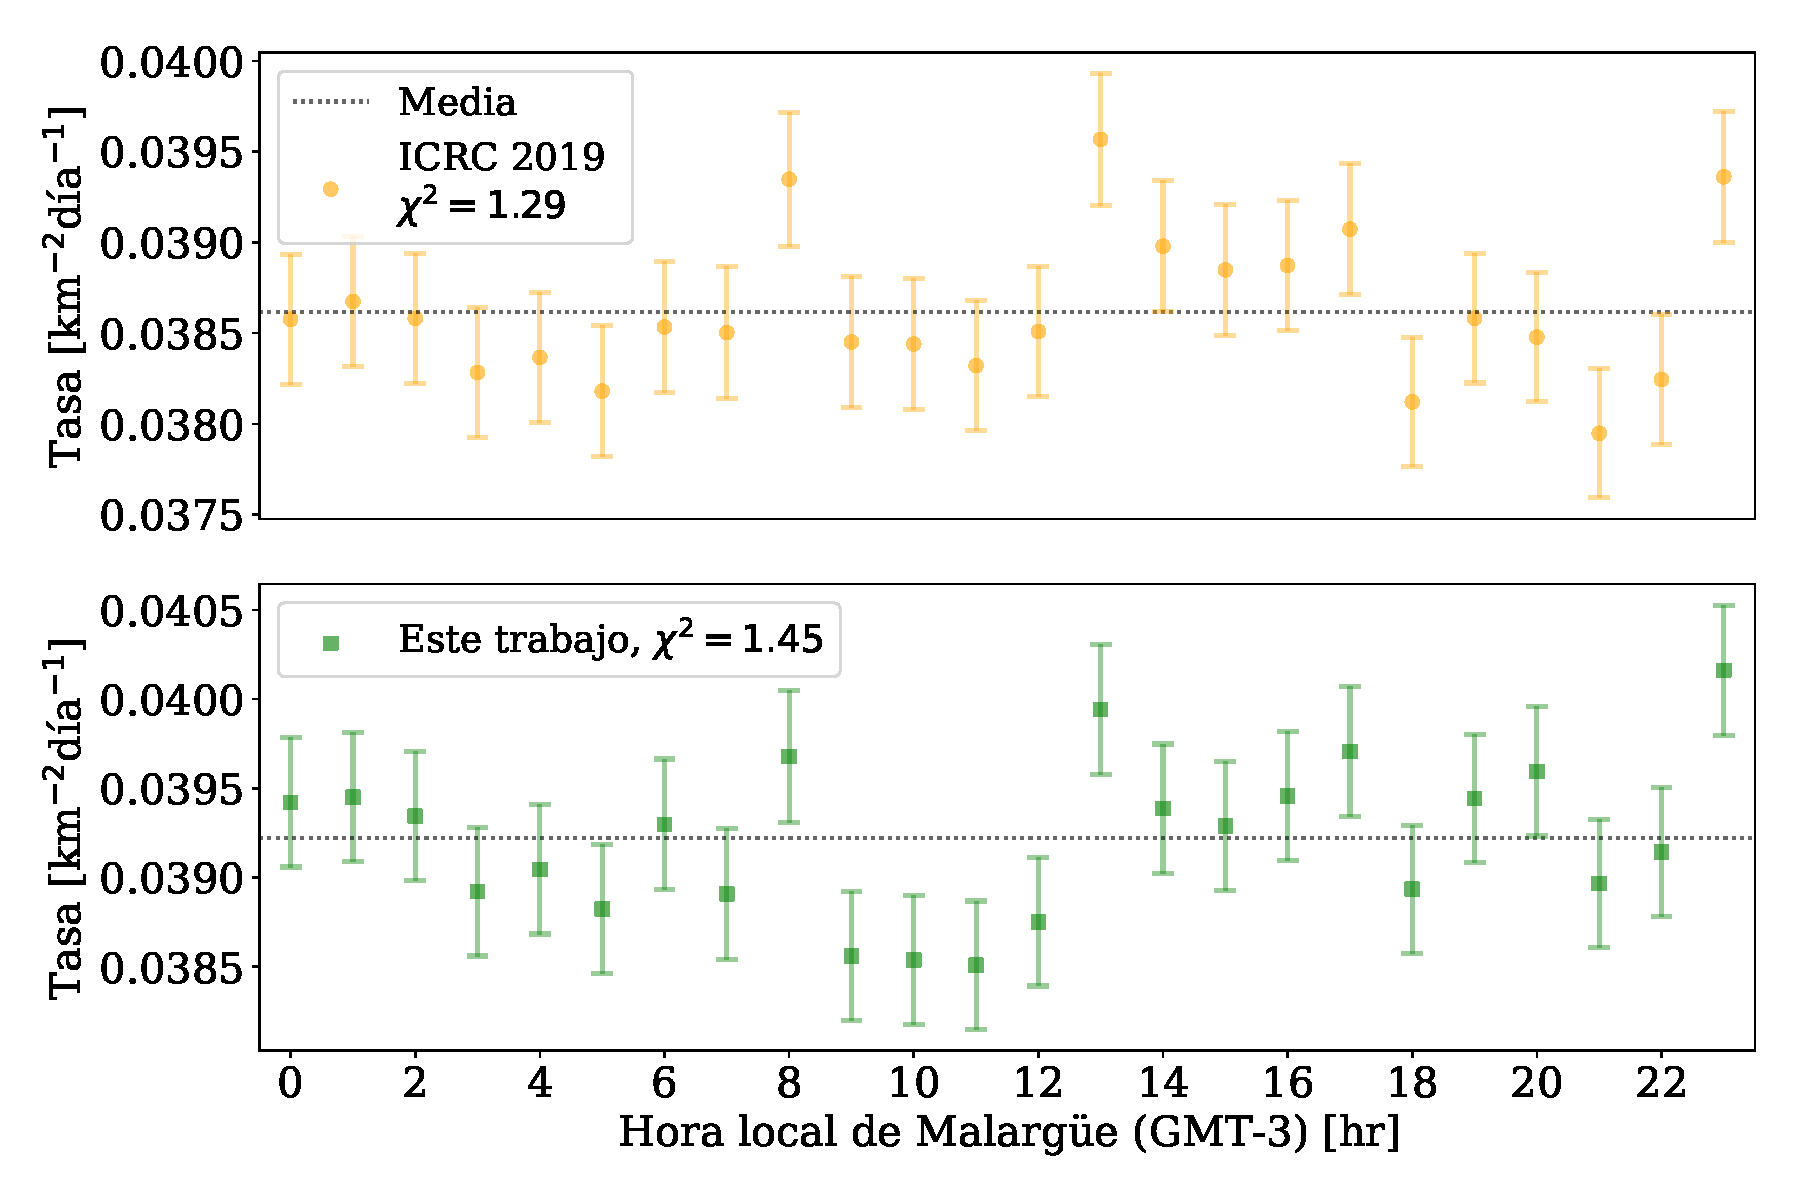
\includegraphics[width=\textwidth]{Graphs/rate_hour_of_the_day/2EeV_ICRC_2019_S38_S1000_expected.pdf}
           \caption{2005-2015} \label{fig:2EeV_expected}
           \end{subfigure}\\
           % \hspace{\fill}
           \begin{subfigure}[b]{0.8\textwidth}
           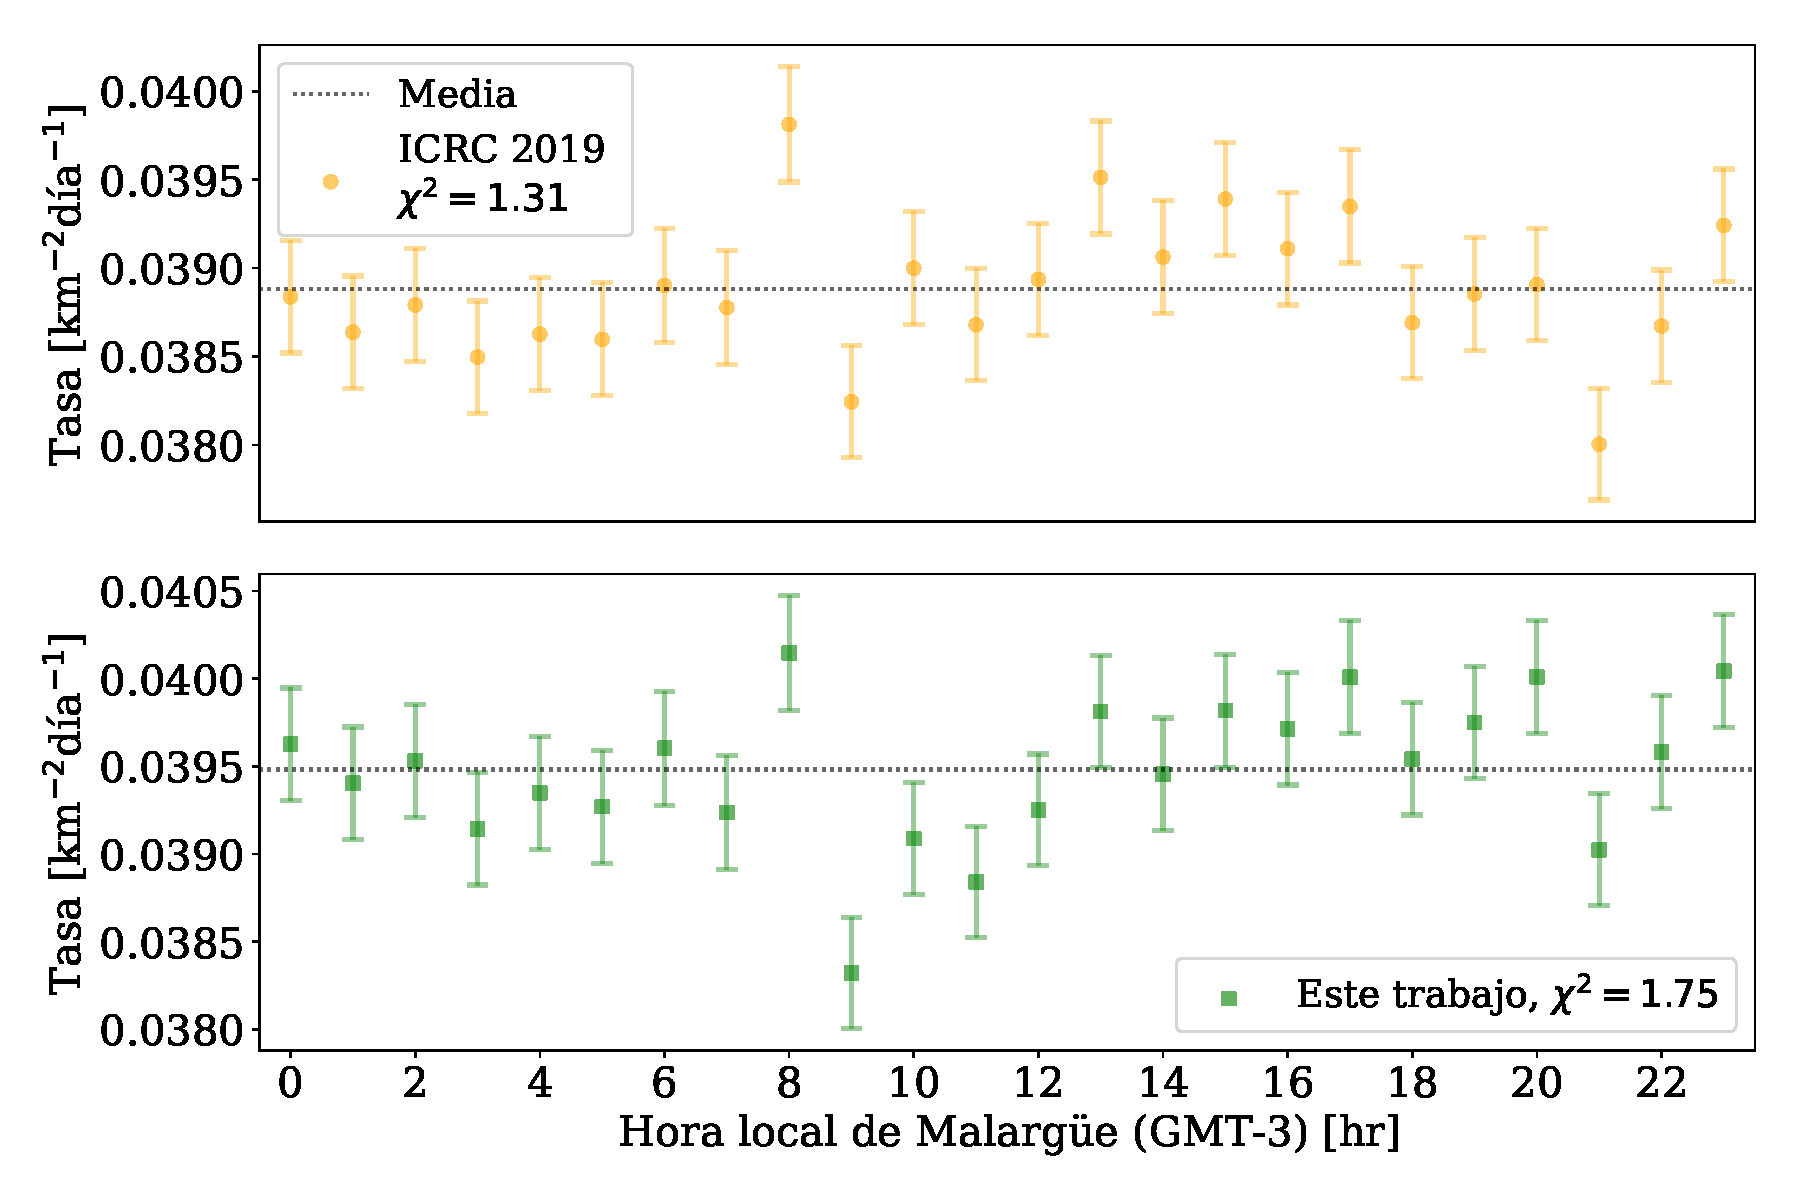
\includegraphics[width=\textwidth]{Graphs/rate_hour_of_the_day/2EeV_ICRC_2019_S38_S1000_expected_05_18.pdf}
           \caption{2005-2018}\label{fig:2EeV_expected_05_18}
           \end{subfigure}%
           \caption{Tasa de eventos por día para eventos de energía mayor a 2\,EeV para los datos de ICRC 2019 y la tasa de eventos obtenida con la reconstrucción de energía en este trabajo comparados en los periodos estudiados}\label{final}
   \end{figure}

	
\section{Eventos asociados a Todos los Disparos en el rango 2014-2020 }	\label{ALL_modulacion}
	

En este trabajo se busca comparar los parámetros obtenidos con los eventos de Todos los Disparos con los parámetros de la reconstrucción oficial. Para esto se realizó un análisis de la señal $S_{38}$ sin la corrección del clima, siguiendo un proceso similar a la sección \ref{sin_corregir_s38}.

\begin{figure}[H]
  \centering
      \begin{subfigure}[b]{0.75\textwidth}
      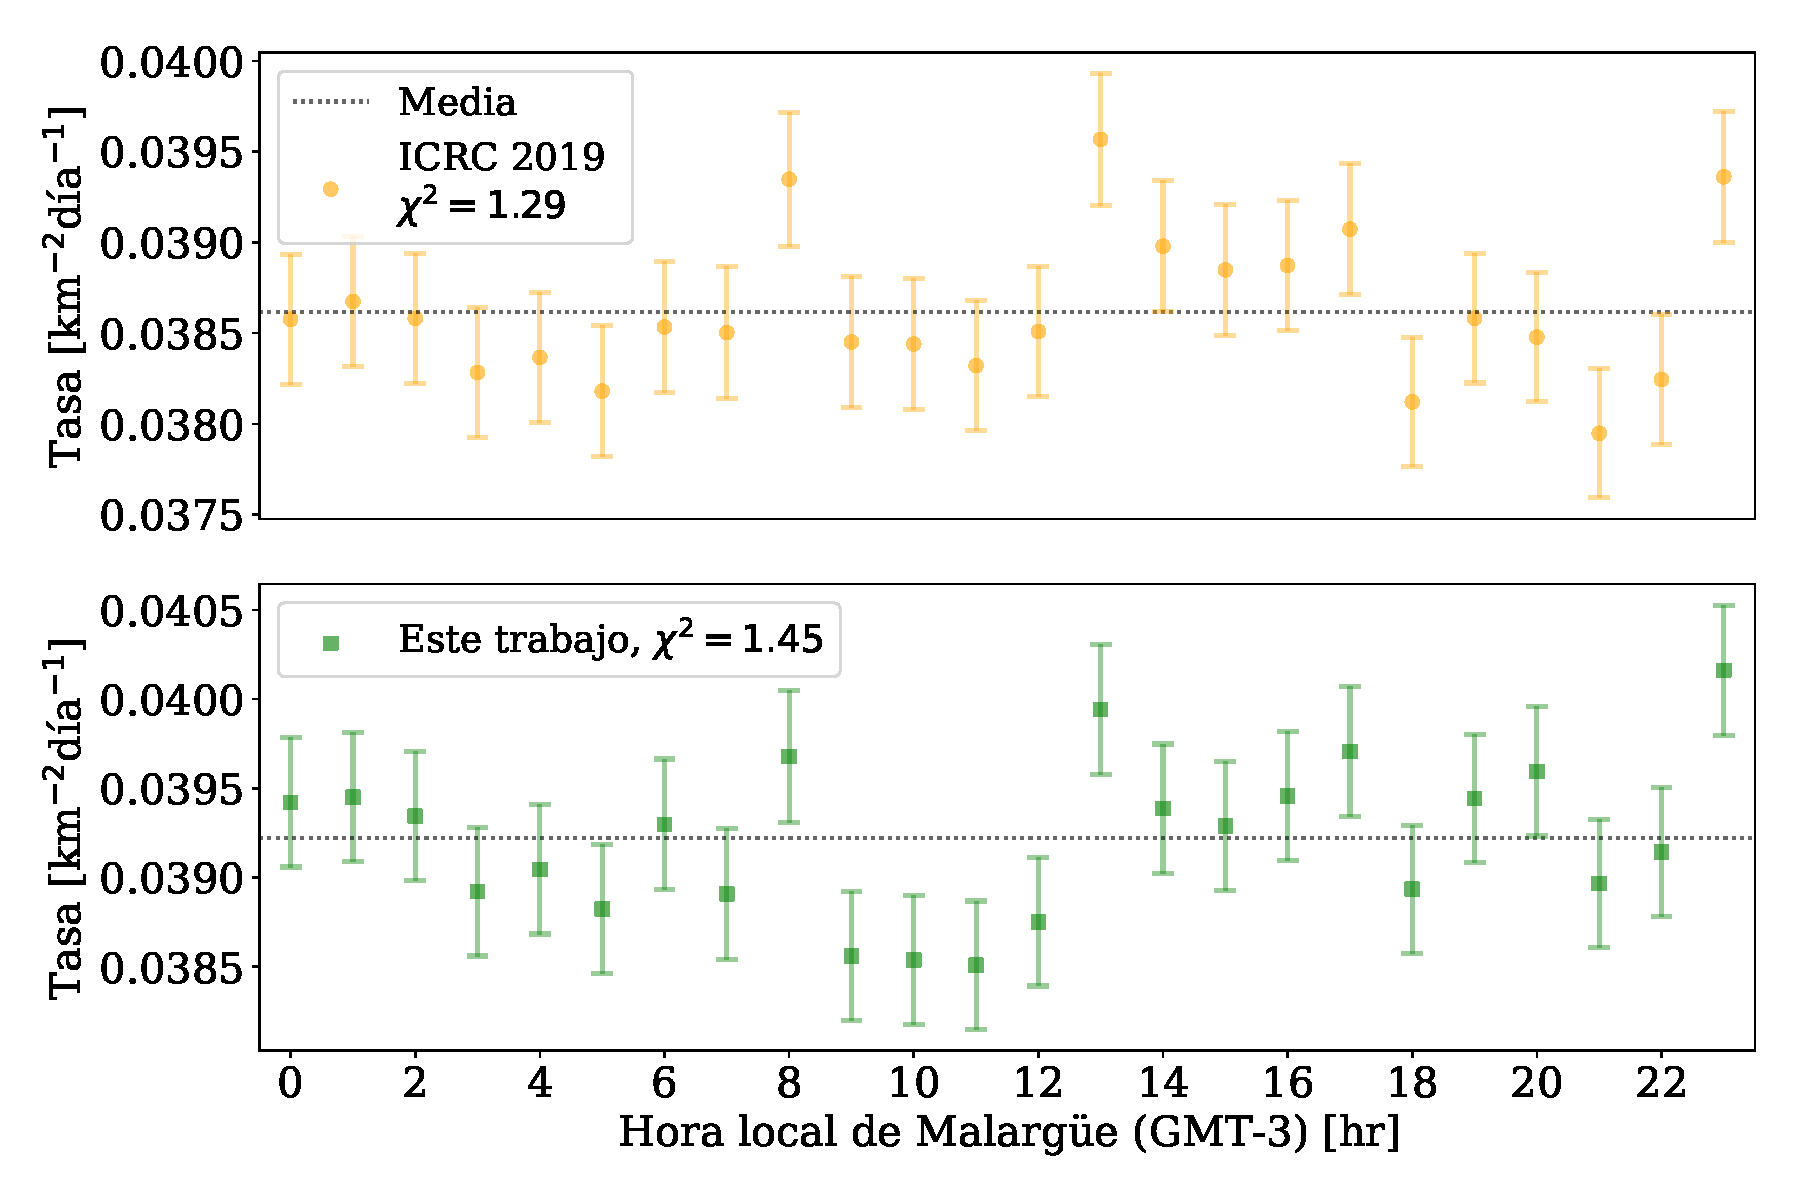
\includegraphics[width=\textwidth]{Graphs/rate_hour_of_the_day/2EeV_ICRC_2019_S38_S1000_expected.pdf}
      \caption{2005-2015} \label{fig:2EeV_expected}
      \end{subfigure}\\
      % \hspace{\fill}
      \begin{subfigure}[b]{0.75\textwidth}
      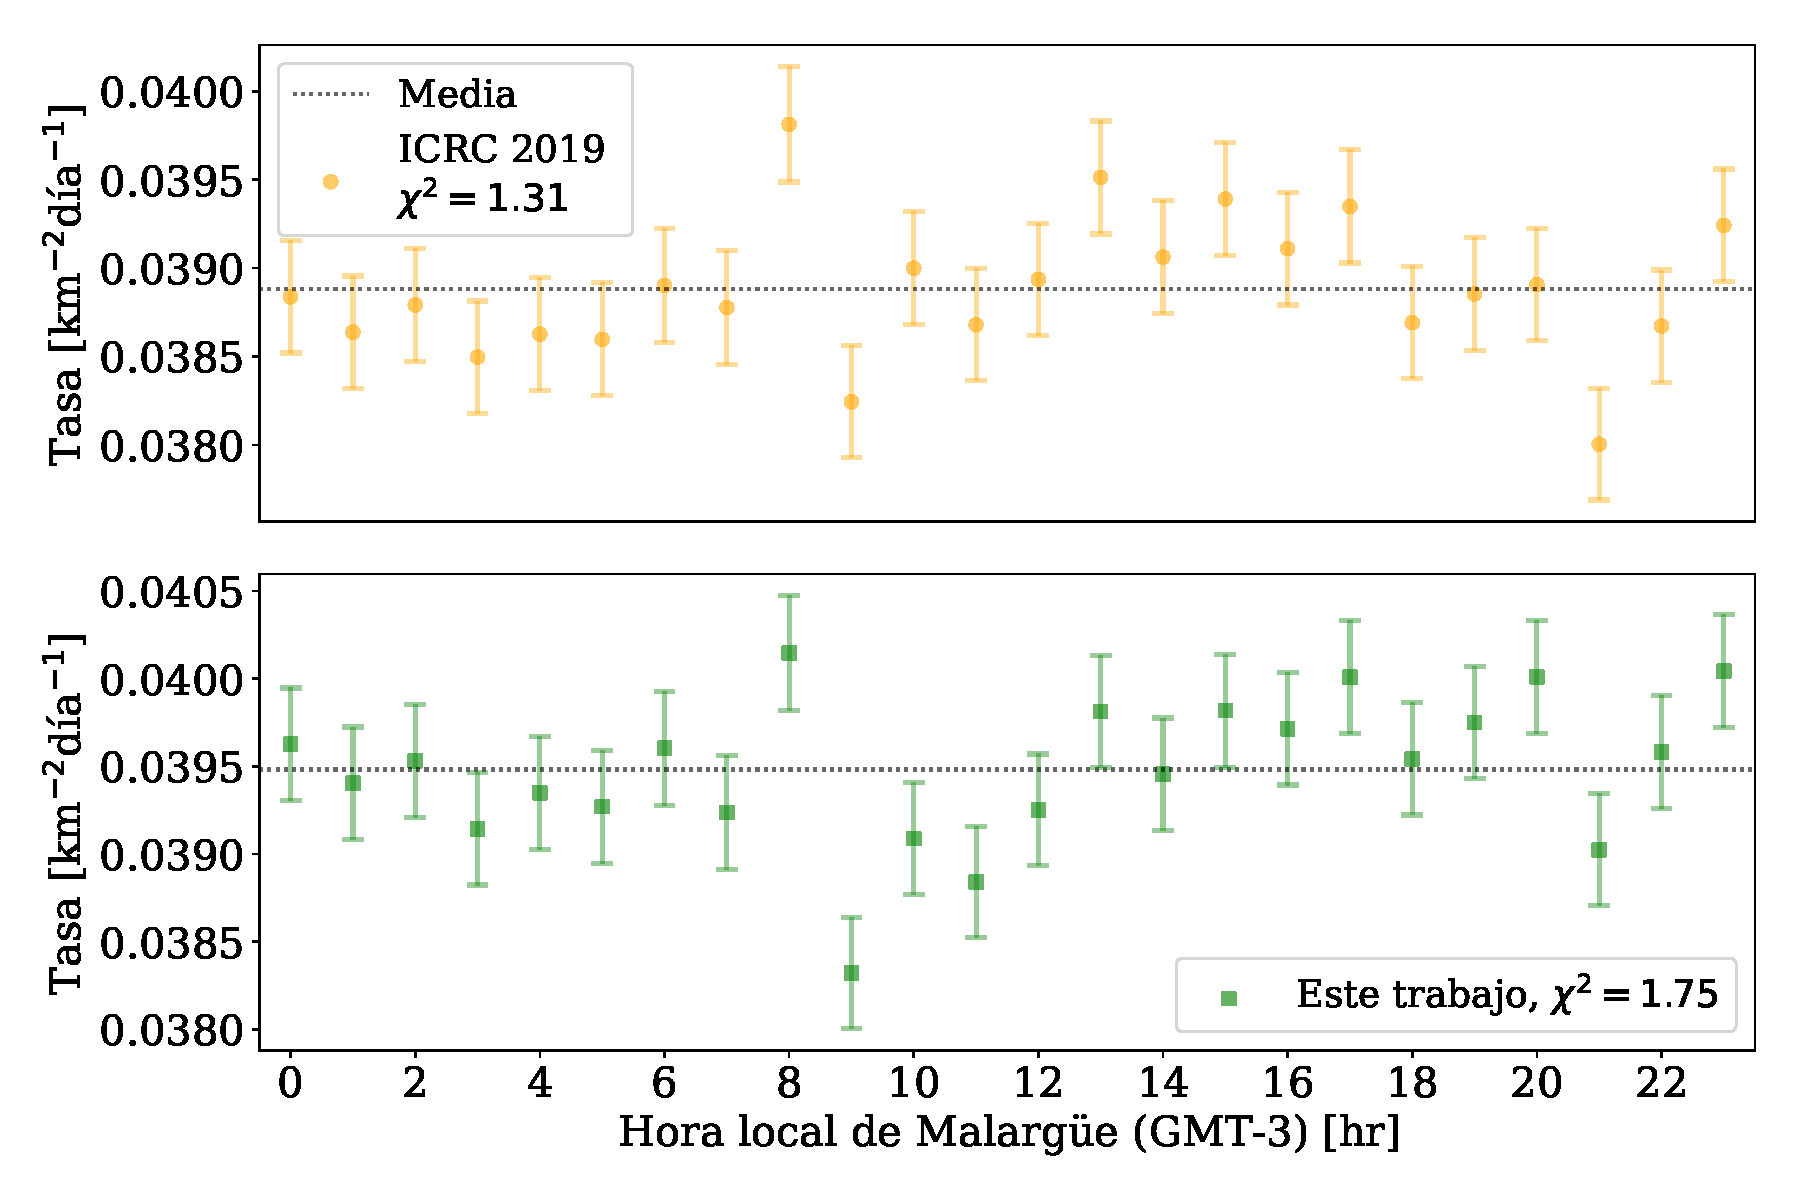
\includegraphics[width=\textwidth]{Graphs/rate_hour_of_the_day/2EeV_ICRC_2019_S38_S1000_expected_05_18.pdf}
      \caption{2005-2018}\label{fig:2EeV_expected_05_18}
      \end{subfigure}%
      \caption{Tasa de eventos por día para eventos de energía mayor a 2\,EeV para los datos de ICRC 2019 y la tasa de eventos obtenida con la reconstrucción de energía en este trabajo comparados en los periodos estudiados}\label{final}
\end{figure}


\subsection{Distribución de los eventos en función de $\sin^2\theta$}

La separación de los eventos en rango de $\sin^2\theta$ para los datos del Disparo Estándar se realizó debido a que distribuye los eventos con energía por encima de $3\,$EeV de forma uniforme en cada rango. En la Fig\,\ref{fig:bin_eventos_sin_2_theta} se muestran las distribuciones que tiene los eventos del Disparo Estándar en distintos rangos de tiempo y los eventos de Todos los Disparos por encima de $3\,$EeV y $1\,$EeV respectivamente. Se toman estos límites porque los disparos alcanzan eficiencia completa a partir de estos valores de energía.  Se observa que para el Disparo Estándar los eventos varian $\sim 2.5\%$ con respecto a la media para los dos rangos de tiempo, en cambio los eventos por encima de $1\,$EeV para Todos los Disparos tienen una variación de $\sim 10\%$ con respecto a media.

\begin{figure}[H]
  \begin{small}
    \begin{center}
      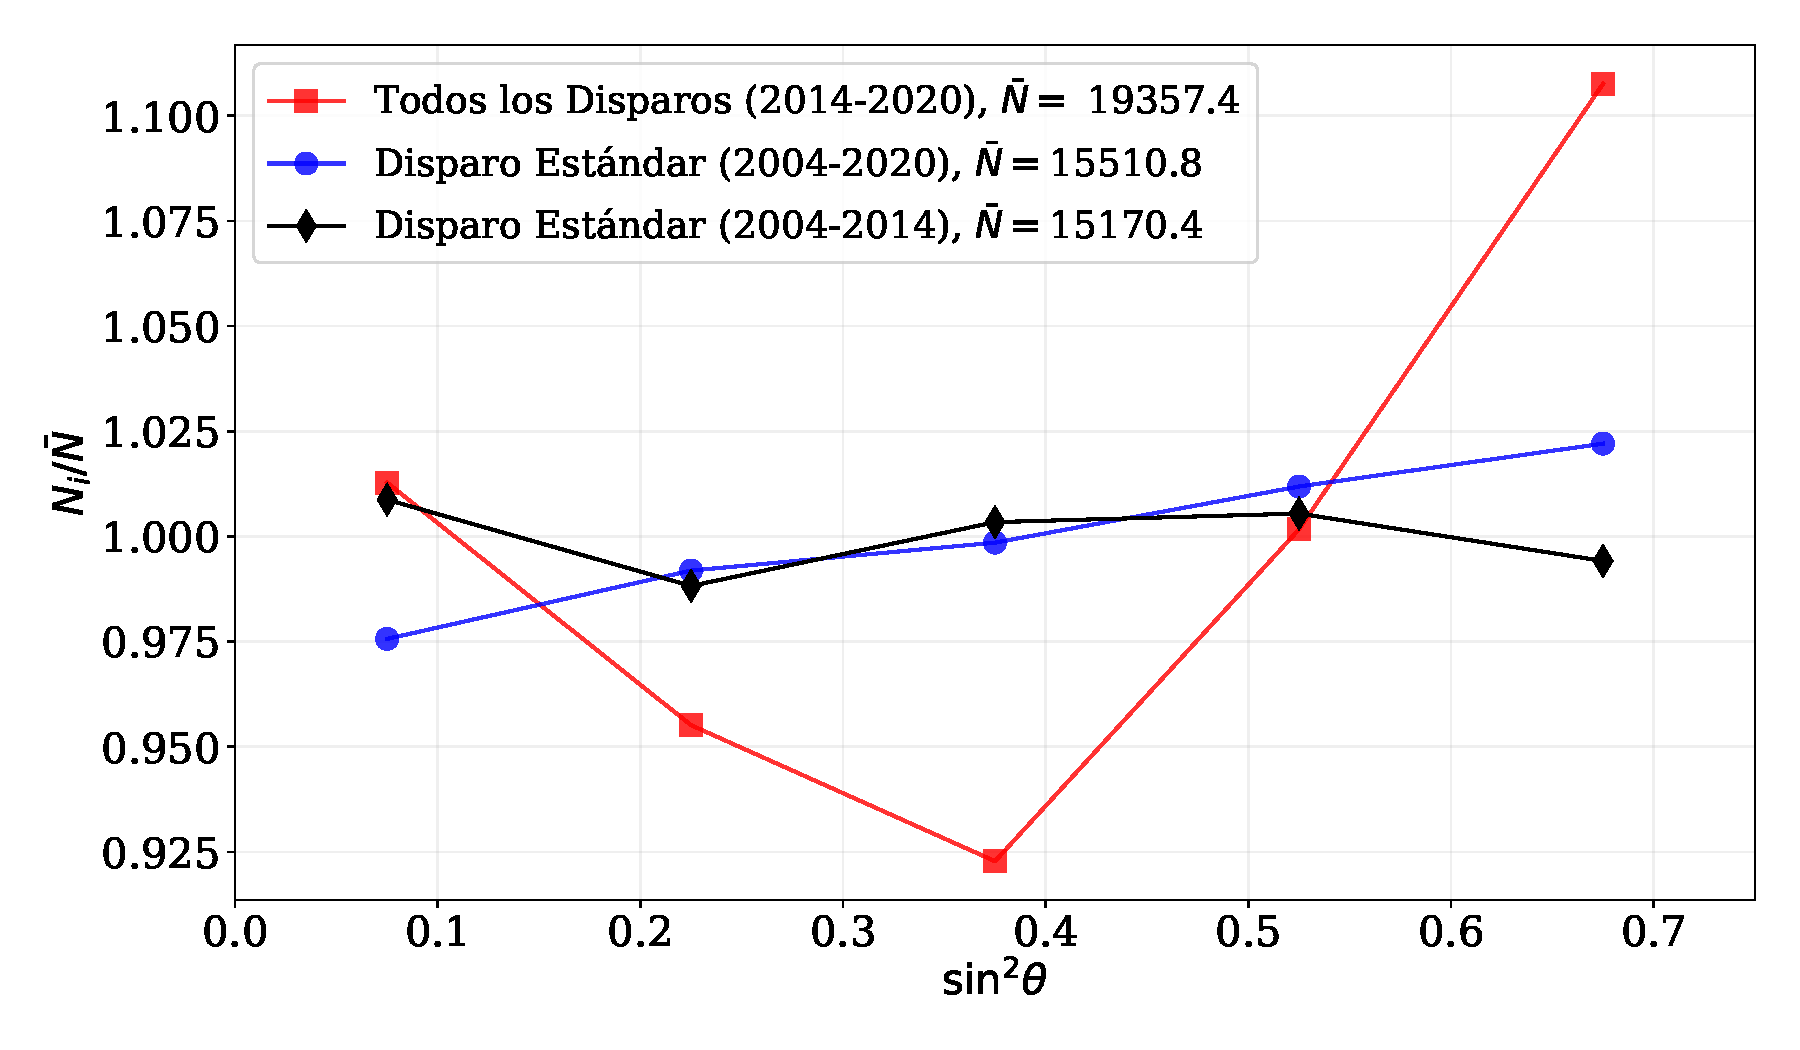
\includegraphics[width=0.8\textwidth]{bin_eventos_sin_2_theta.pdf}
    \end{center}
    \caption{Variación de eventos en cada rango de $\sin^2\theta$ respecto a la media para el Disparo Estándar y Todos los Disparos. }
    \label{fig:bin_eventos_sin_2_theta}
  \end{small}
\end{figure}
\subsection{Tasa de eventos de Todos los Disparos por encima de 1 EeV}

Los eventos de este conjunto de datos, la modulación espuria del clima está corregida con los parámetros obtenidos sobre el Disparo Estándar. Las tasas de eventos diario mostrados en la Fig.\,\ref{fig:rate_ALL}, por encima de 1 EeV y 2 EeV respectivamente, no muestran modulaciones importantes. En el caso de la tasa por encima de 1 EeV, se observa un remanente de modulación anual similar a los datos del ICRC 2019. 





\subsection{Parámetros del clima para Todos los Disparos usando $S_{38}$}


En esta sección, se trabajó con el conjunto de datos registrados por el arreglo principal con Todos los Disparos. La señal de $S(1000)$ de estos eventos fue corregida en la reconstrucción oficial de eventos por la modulación del clima por los parámetros obtenidos en \cite{aab2017impact}, por este motivo se trabajó con un corte en la señal de $S_{38}$ sin corregir por el clima. Las características de eventos obtenidos con el corte en la señal y otros filtros mencionados se resumen en la Tabla~\ref{tabla:caracteristicas_ALL}. 

\begin{figure}[H]
  \centering
  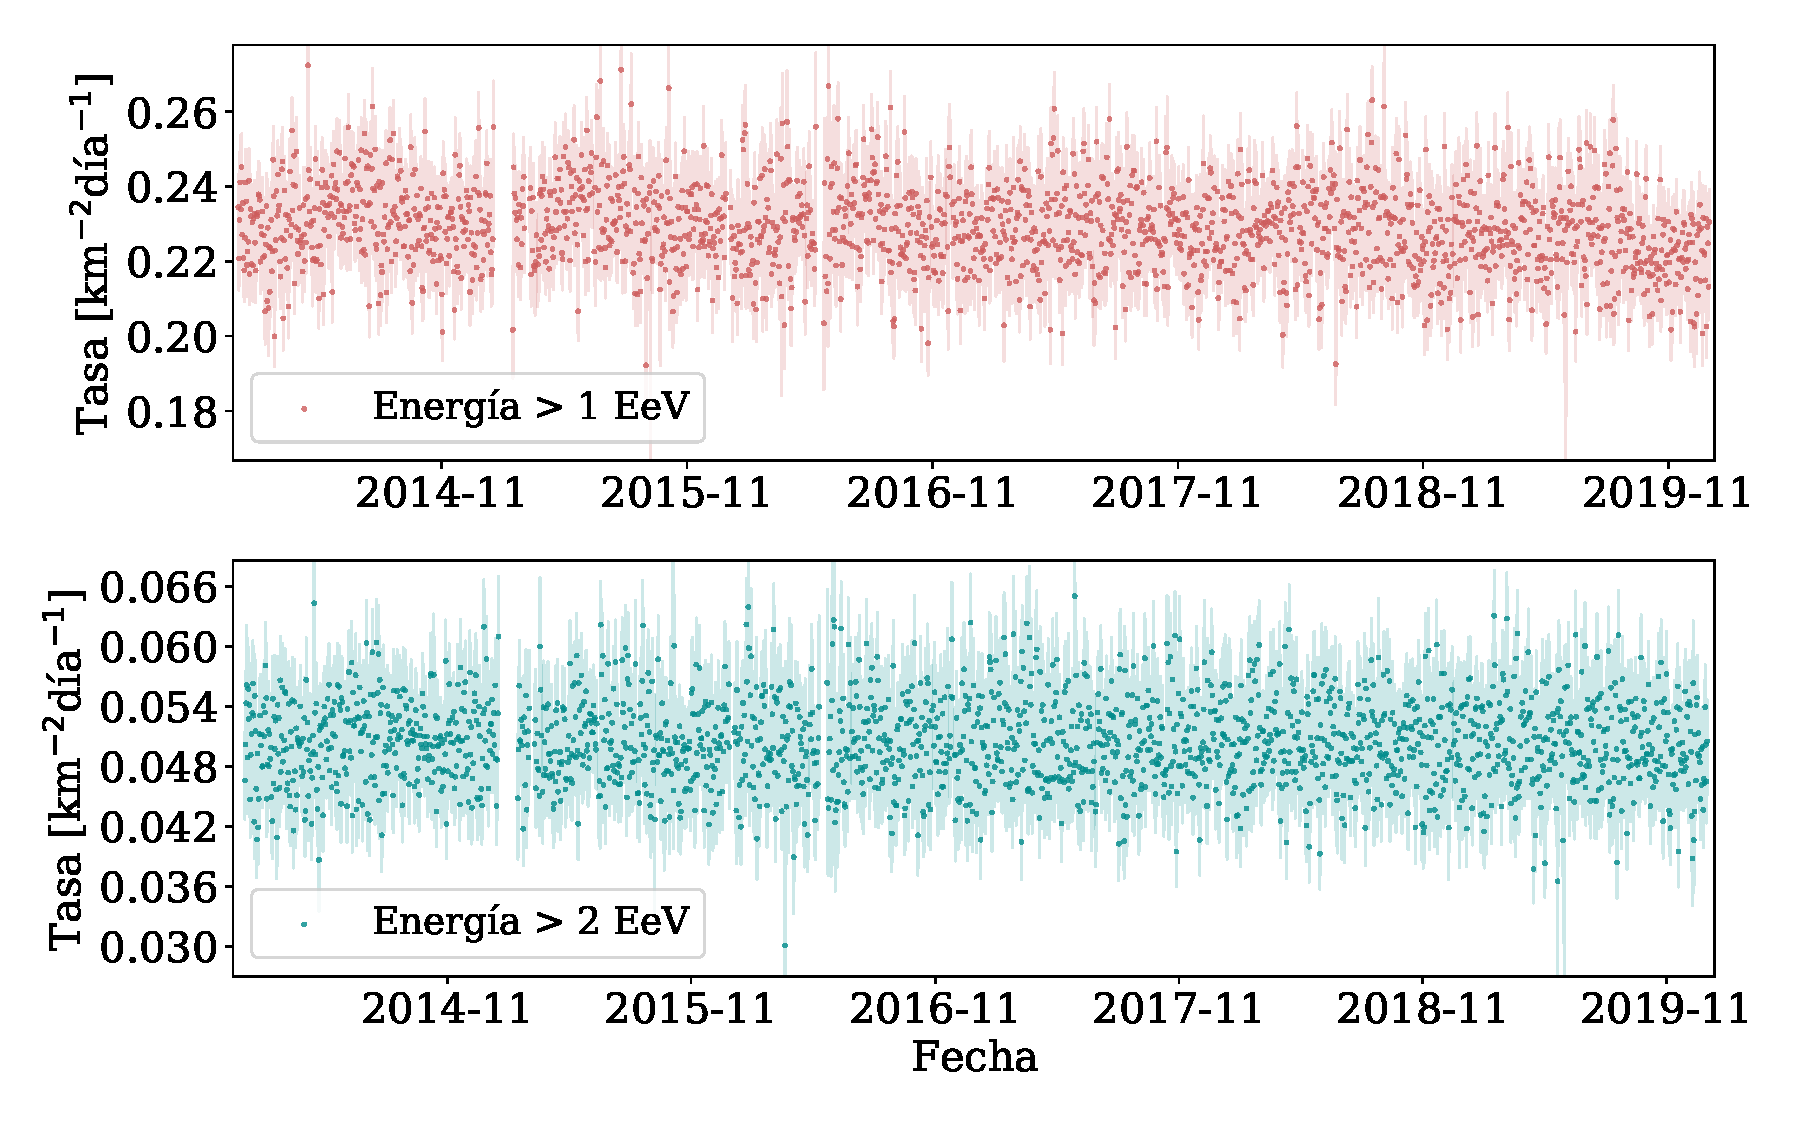
\includegraphics[width=0.8\textwidth]{../04_Clima/Graphs/rate_dayly/AllTriggers_1EeV_2EeV_rate.pdf}
  \caption{Tasa de eventos promedio por cada día desde inicios del 2005 hasta inicios del 2020 de Todos los Disparos. Se muestran las tasas para dos cortes en energía, mayor a $1\,$EeV y mayor a $2\,$EeV}\label{fig:rate_ALL}
\end{figure}

\begin{table}[H]
  \centering
  \begin{tabular}{r|c|}
    \cline{2-2}
                & Todos los Disparos \\ \cline{2-2}
  Inicio:              & 01/01/2014\\ 
  Final:               & 01/01/2020       							\\ 
  Número de eventos:   & 1\,263\,015							\\ 
  Energía media:       & 1.76\,EeV       				\\  %  1.005\,EeV
  Corte en $S_{38}$:   & $>$5.37 VEM        				\\ 
  Corte en ángulo cenital:& $\theta < 60^o$ 				\\ \cline{2-2}
  \end{tabular}
\caption{Características del conjunto de datos de Todos los Disparos.} \label{tabla:caracteristicas_ALL}
\end{table}

Se realiza un ajuste de la tasa de eventos de Todos los Disparos y de esta manera se obtienen los coeficientes promediados por ángulo cenital. Los parámetros obtenidos se presentan y se comparan con los obtenidos sobre eventos del Disparo Estándar \cite{aab2017impact} en la Tabla \ref{tabla:parametros_ALL}. Los errores presentados son los errores obtenidos por el ajuste.  

\begin{table}[H]
  \centering
  \begin{tabular}{c|c|c}
  {Parámetro}                 & Todos los Disparos (2014-2020)& {2005-2015}    \cite{aab2017impact}              \\ \hline \hline
  $a_P$ [hPa$^{-1}$]          & $(-4.8 \pm 0.2)\times 10^{-3}$& $(-3.2 \pm 0.3)\times 10^{-3}$    \\ \hline
  $a_\rho$ [kg$^{-1}$m$^3$]   & $-1.54 \pm 0.04 $             & $-1.72 \pm 0.04$                  \\ \hline
  $b_\rho$ [kg$^{-1}$m$^3$]   & $-0.55 \pm 0.04$              & $-0.53 \pm 0.04$                  \\ \hline
  $\chi^2_\nu$                & $1.016$                       & $1.013$                           \\ 
  \end{tabular} 
  \caption{Ajustes obtenidos considerando todos los eventos con $\theta<60^o$ y energía mayor a $1\,$EeV del conjunto de Todos los disparos, comparados con los parámetros utilizados por la Colaboración \cite{aab2017impact}.} \label{tabla:parametros_ALL}
\end{table}


La tasa de eventos media por día  medida y la tasa predicha según los parámetros del clima obtenidos se observan en la Fig.\ref{fig:rate_dayly_AllTriggers}. En la misma, la modulación anual y diaria del clima sobre los eventos es apreciable, a diferencia de las tasas de la Fig.\,\ref{fig:rate_ALL} donde  la energía de estos eventos están corregidos.  
\begin{figure}[H]
\centering
  \begin{subfigure}[b]{0.9\textwidth}
  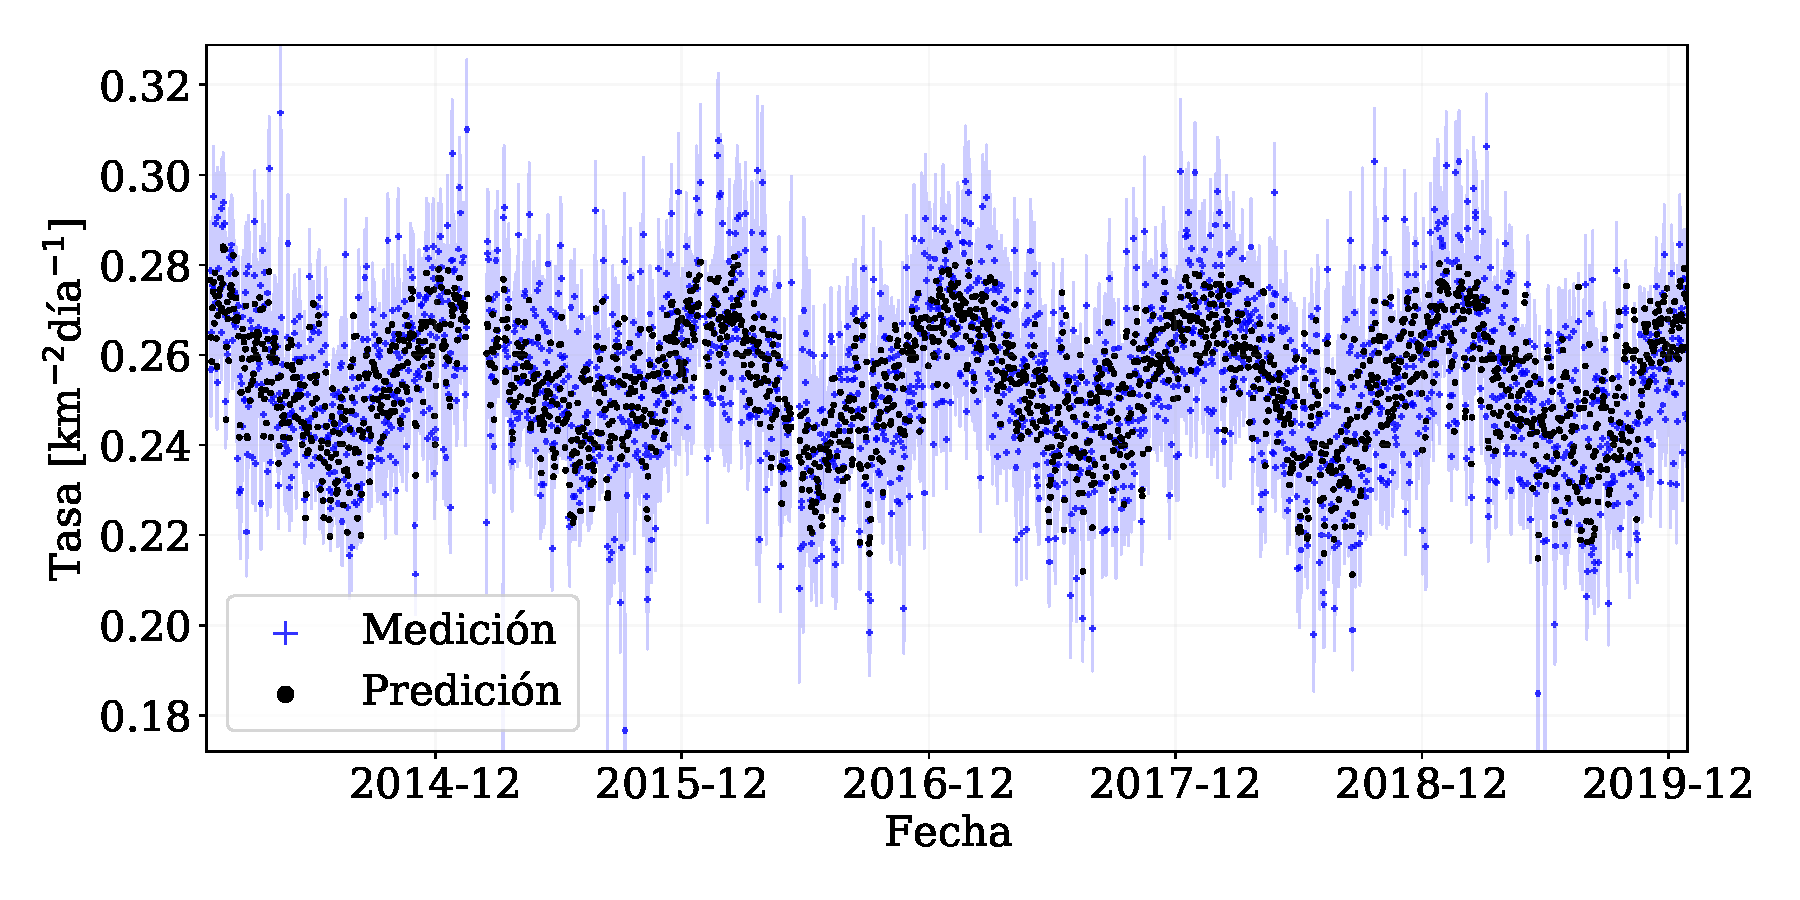
\includegraphics[width=\textwidth]{Graphs/rate_dayly/AllTriggers_S38_over_1EeV_rate_v3.pdf}
  \caption{Tasa eventos por día}\label{fig:rate_dayly_AllTriggers}
  \end{subfigure}\\
  \begin{subfigure}[b]{0.9\textwidth}
  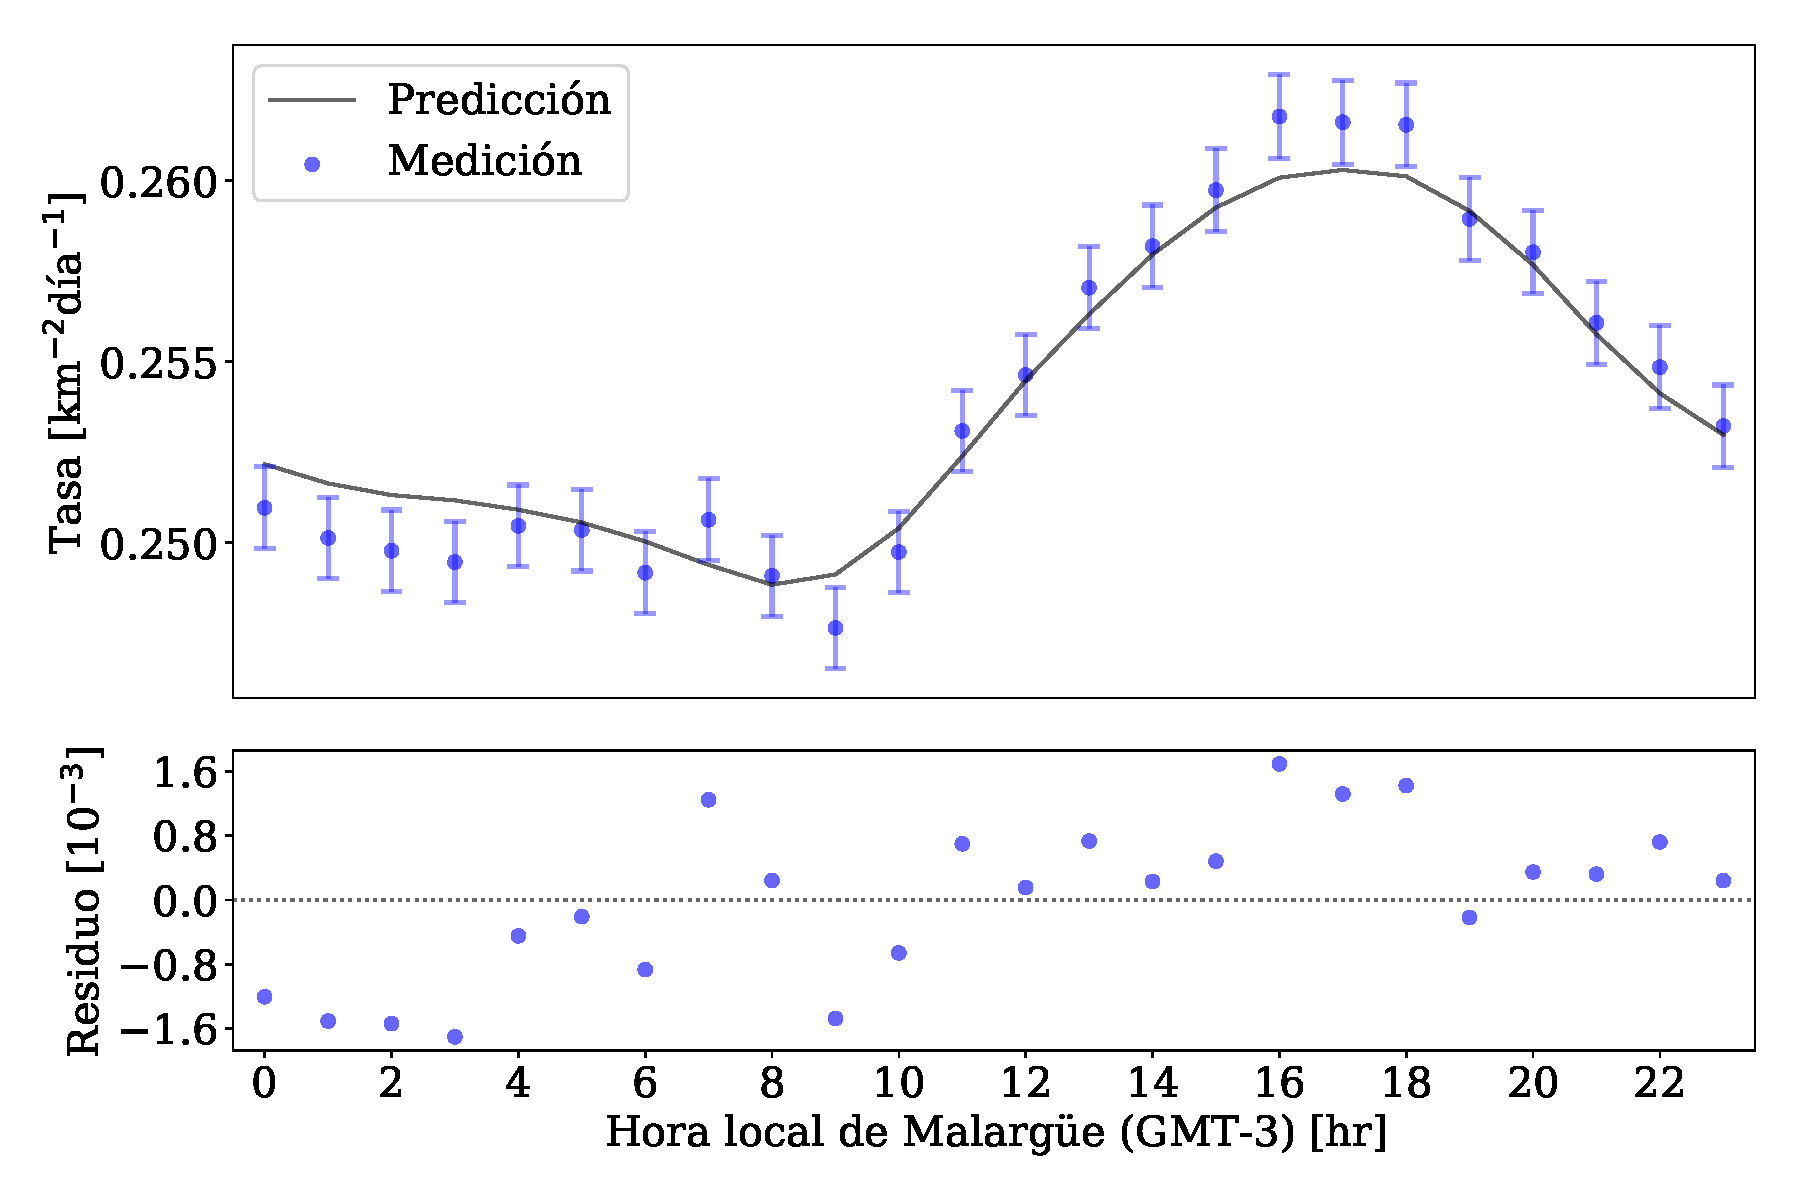
\includegraphics[width=\textwidth]{Graphs/rate_hour_of_the_day/AllTriggers_S38_over_1EeV_hour_of_the_day.pdf}
  \caption{Tasa de eventos promediada por hora del día }\label{fig:rate_hod_AllTriggers}
  \end{subfigure}
  \caption{Tasa de eventos por días comparadas con el ajuste entre los años 2014 hasta 2020. Estos eventos se registraron con Todos los Disparos  y tienen un valor de $S_{38}$ mayor a $5.37\,$VEM. En las tasas se observan la modulación anual y diaria del clima. La predicción es obtenida por los parámetros calculados en este trabajo.}\label{fig:rate__AllTriggers}
\end{figure}

Para poder verificar que los parámetros del clima en función de $\sin^2\theta$ obtenidos sobre el Disparo Estándar son válidos para Todos los Disparos, se calculó estos parámetros del último y se compararon con los utilizados por la Colaboración en la reconstrucción oficial. Estos resultados se observan en la Fig.\,\ref{fig:ALL-params} y los ajustes de la Ec.\,\ref{eq:cuadratica} se presentan en la Tabla~\ref{tabla:cuadratica_ALL}.   

\begin{figure}[H]
  \centering
  \begin{subfigure}[b]{0.8\textwidth}
  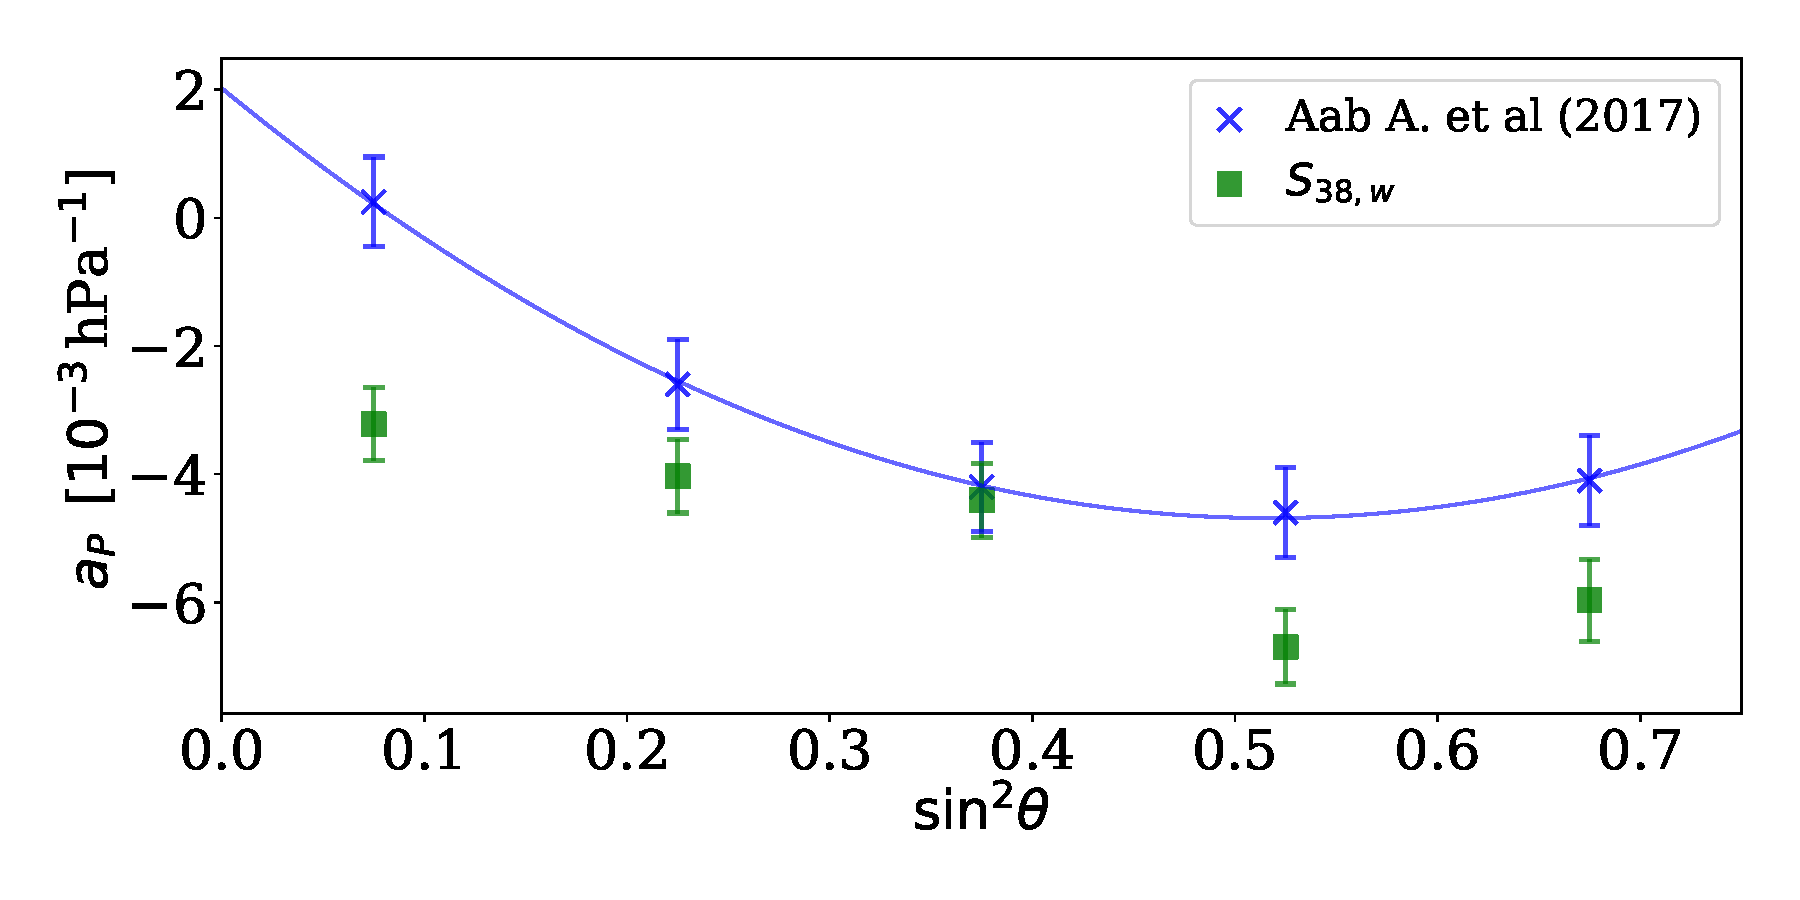
\includegraphics[width=\linewidth]{Graphs/params/ap_AllTriggers.pdf}
  \caption{Parámetro $a_P$ }
  \end{subfigure}\\
  \begin{subfigure}[b]{0.8\textwidth}
  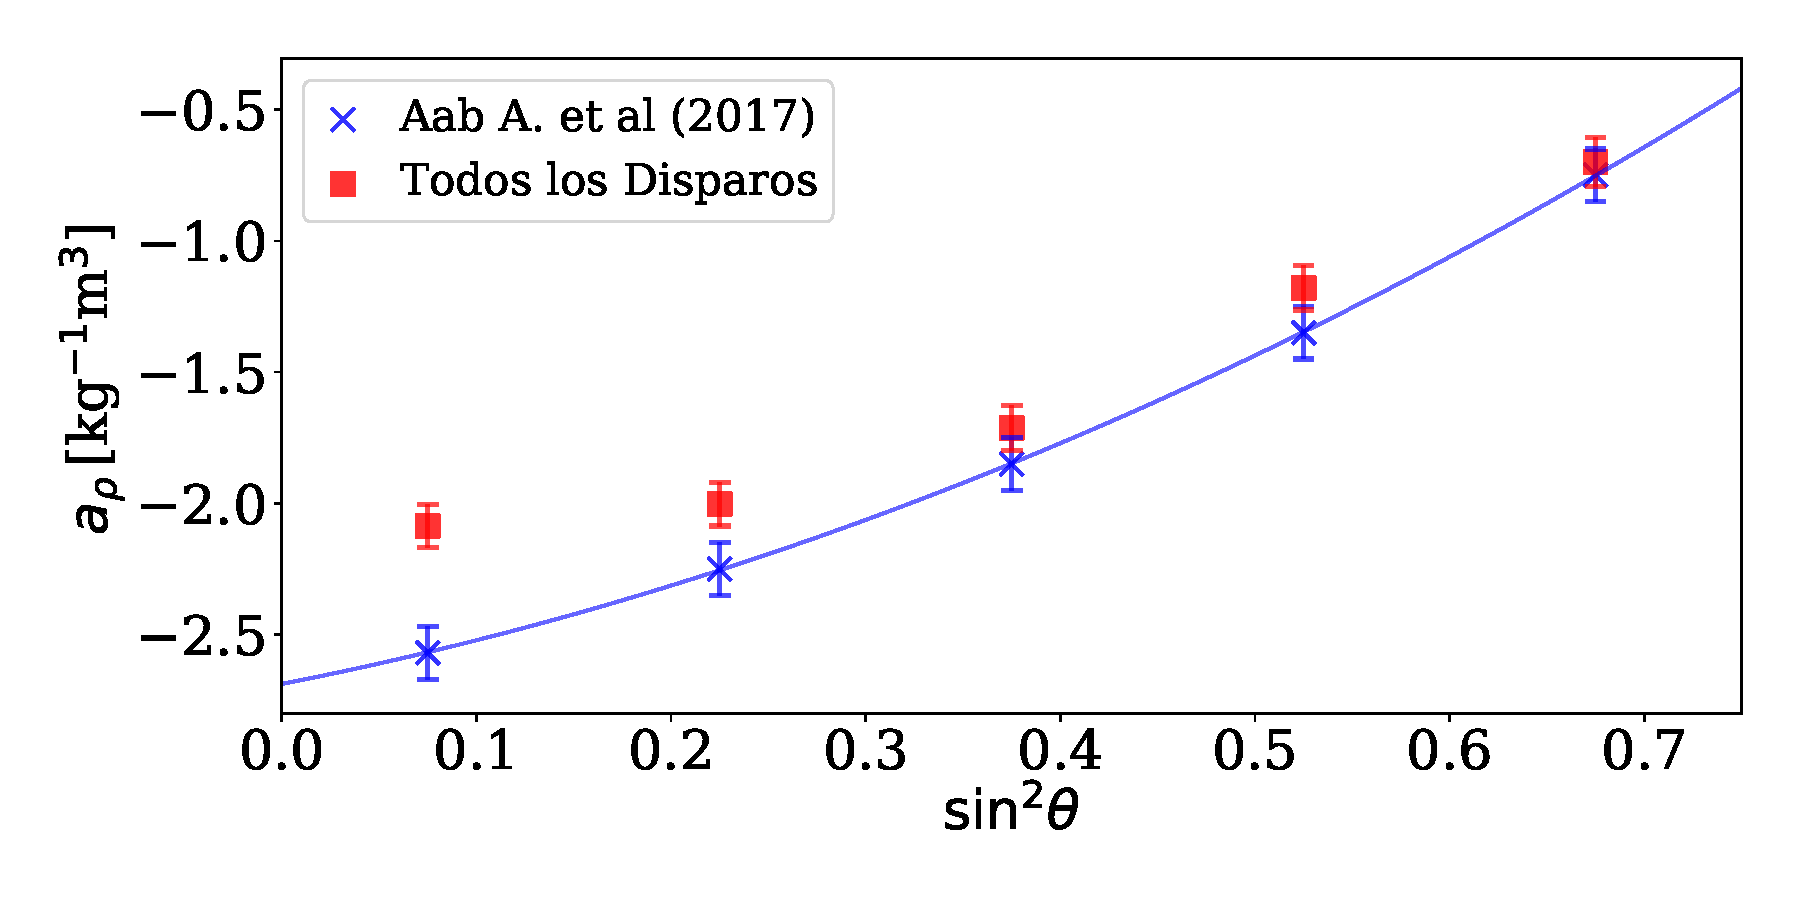
\includegraphics[width=\linewidth]{Graphs/params/arho_AllTriggers.pdf}
  \caption{Parámetro $a_{\rho}$ }
  \end{subfigure}\\
  \begin{subfigure}[b]{\textwidth}
  \centering
  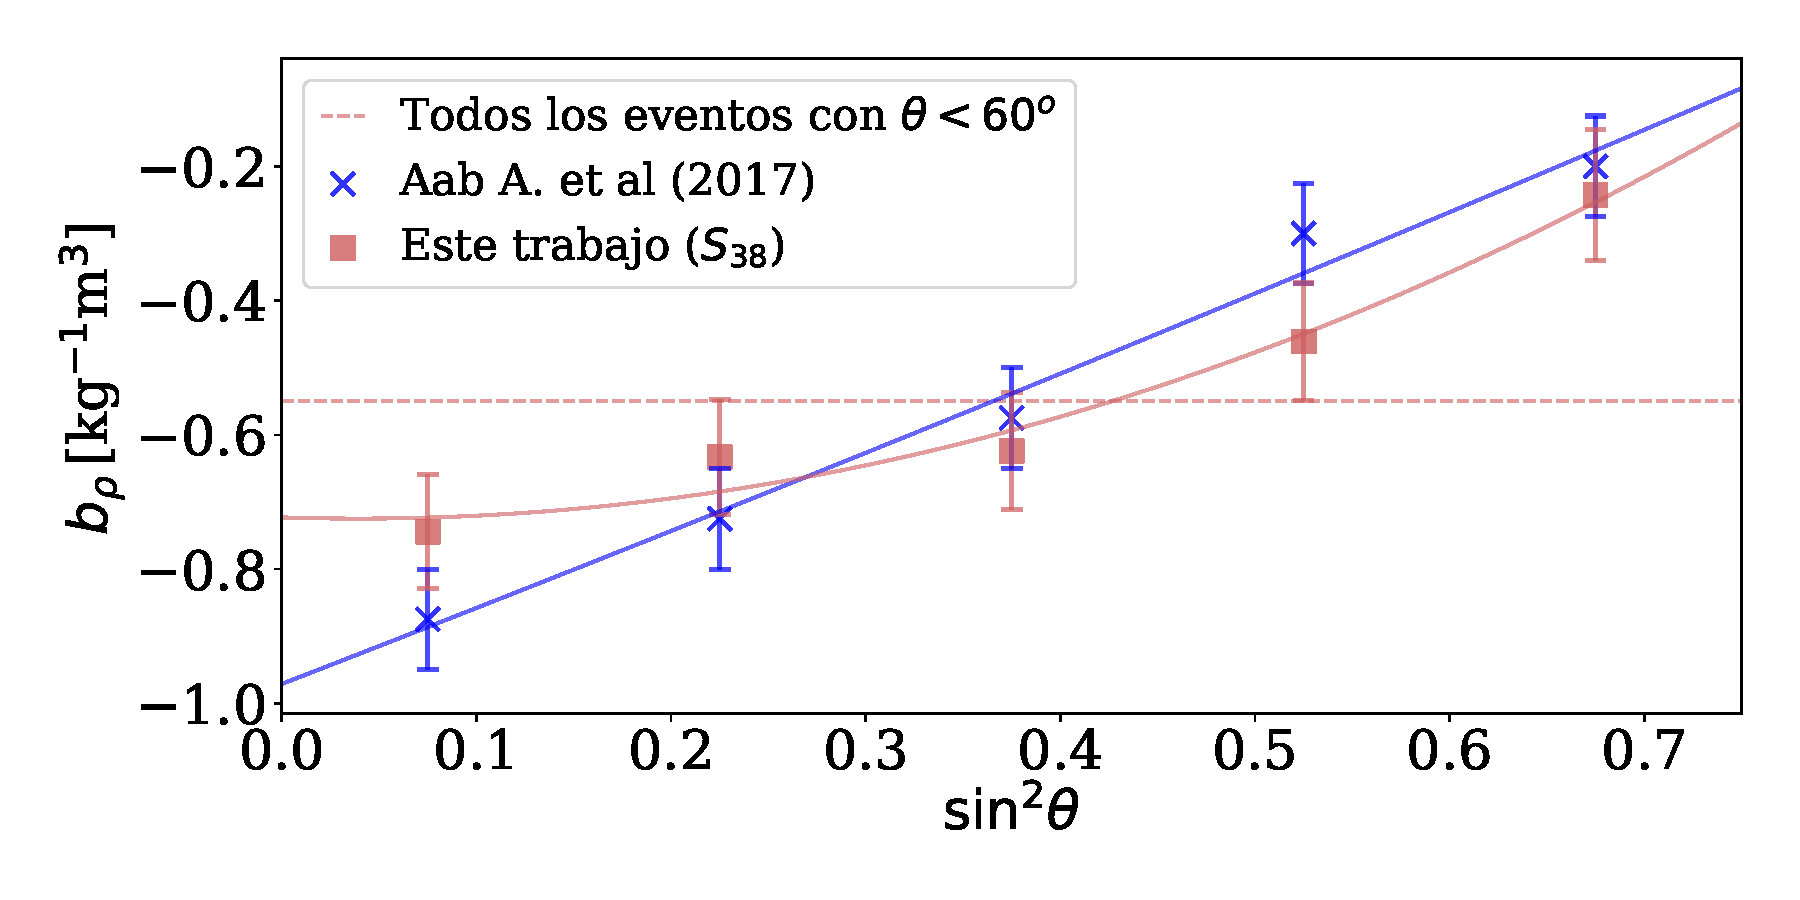
\includegraphics[width=0.8\linewidth]{Graphs/params/brho_AllTriggers.pdf}
  \caption{Parámetro  $b_\rho$   }
  \end{subfigure}
  \caption{Parámetros de la modulación del clima considerando los datos de Todos los Disparos, obtenido en el rango 2014-2020 . Los mismos se comparan con los coeficientes utilizados por la Colaboración \cite{aab2017impact}.}
  \label{fig:ALL-params}
\end{figure}

\begin{table}[H]
  \centering
  \begin{tabular}{l|l|l|l}
       Parámetros									& Coeficiente		& Todos los Disparos (2014-2020)	                  & \cite{aab2017impact}	\\ \hline \hline
   \multirow{3}{*}{$a_P$ [hPa$^{-1}$]}  			    &  $c_0$			& $( 2.5\pm 1.2)\times 10^{-3}$	& $( 2.1 \pm 0.9)\times 10^{-3} $	\\ \cline{2-4} %Done
                                                  &  $c_1$			& $(-8 \pm 8)\times 10^{-3}$	& $(-26.0 \pm 0.6 )\times 10^{-3}$	\\ \cline{2-4} 
                                                  &  $c_2$			& $( 0.0\pm 1.0)\times 10^{-3}$	& $( 26.0 \pm 0.7 )\times 10^{-3}$	\\ \hline \hline% 
  
   \multirow{3}{*}{$a_\rho$ [kg$^{-1}$m$^3$]}  	  &  $c_0$			& $-2.07   \pm 0.09$	            & $ -2.7  \pm 0.1  $\\ \cline{2-4} 
                                                  &  $c_1$			& $-0.0    \pm 0.5 $	            & $ 1.5   \pm 0.8  $\\ \cline{2-4} 
                                                  &  $c_2$			& $ 3.3    \pm 0.8 $	            & $ 2.2   \pm 1.0  $\\ \hline \hline%
  
  \multirow{3}{*}{$b_\rho$ [kg$^{-1}$m$^3$]} 		  &  $c_0$			& $-0.72   \pm 0.07$		            & $-1.0   \pm 0.1 $	\\ \cline{2-4} 
                                                  &  $c_1$			& $-0.0    \pm 0.4$		            & $ 1.2   \pm 0.8  $	\\ \cline{2-4} 
                                                  &  $c_2$			& $ 1.1    \pm 0.6$		            & $ 0.0   \pm 1.1  $	\\ 
  
  \end{tabular}	
  \caption{Tabla de los coeficientes obtenidos para Todos los Disparos, comparados con los parámetros de la reconstrucción de los eventos del Observatorio.} \label{tabla:cuadratica_ALL}
\end{table}


% \subsection{Pesos de los hexágonos en el rango 2014-2020}

% Para constatar que no exista ninguna anomalía en los pesos de los hexágonos, se realiza el cálculo de los mismos para tres frecuencias de referencia para el análisis de anisotropías.  Los pesos se muestran en la Fig.\,\ref{fig:wei_14_20}. El rango de tiempo en el que se calculan estas curvas es entre 1 de Enero del 2014 y el 1 de Enero del 2020.

% \begin{figure}[H]
% 	\centering
% 	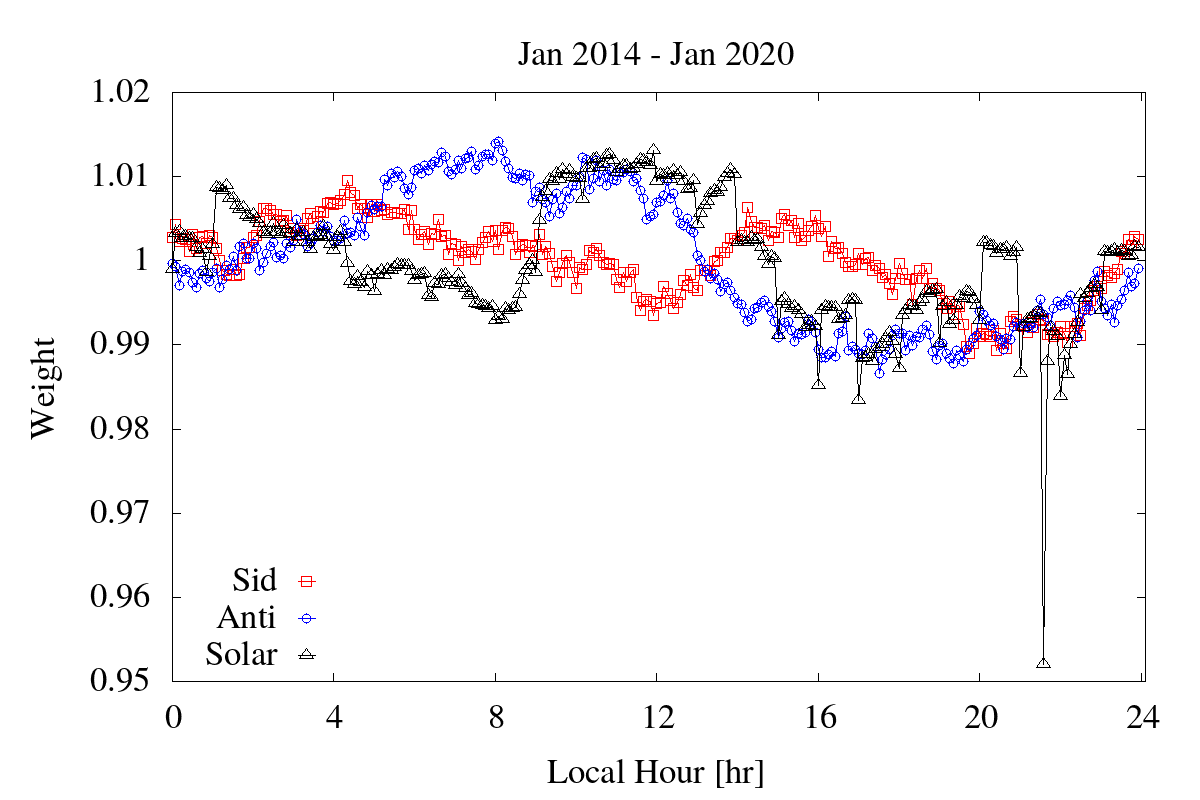
\includegraphics[width=0.5\textwidth]{weigth2014-2020_jan.png} 	
% 	\caption{Pesos de los hexágonos}
% 	\label{fig:wei_14_20}
% \end{figure}



      % Considerando el filtro con el S38 en el archivo 2020 y la energía en el 2017, quiero saber si obtengo parámetros  del clima comparables. Ya que el Main Array se corresponden los parámetros del 2015 y 2019, yo esperaría que con todos los triggers pase los mismo. Una diferencia importante entre ambos análisis es que los parámetros del 2020 contienen eventos hasta el 31/12/2019.
      
      % Los mismos se comparan con los ajustes obtenidos en \cite{aab2017impact}.

        % \begin{figure}[H]
        %   \centering
        %   \begin{subfigure}[b]{0.75\textwidth}
        %   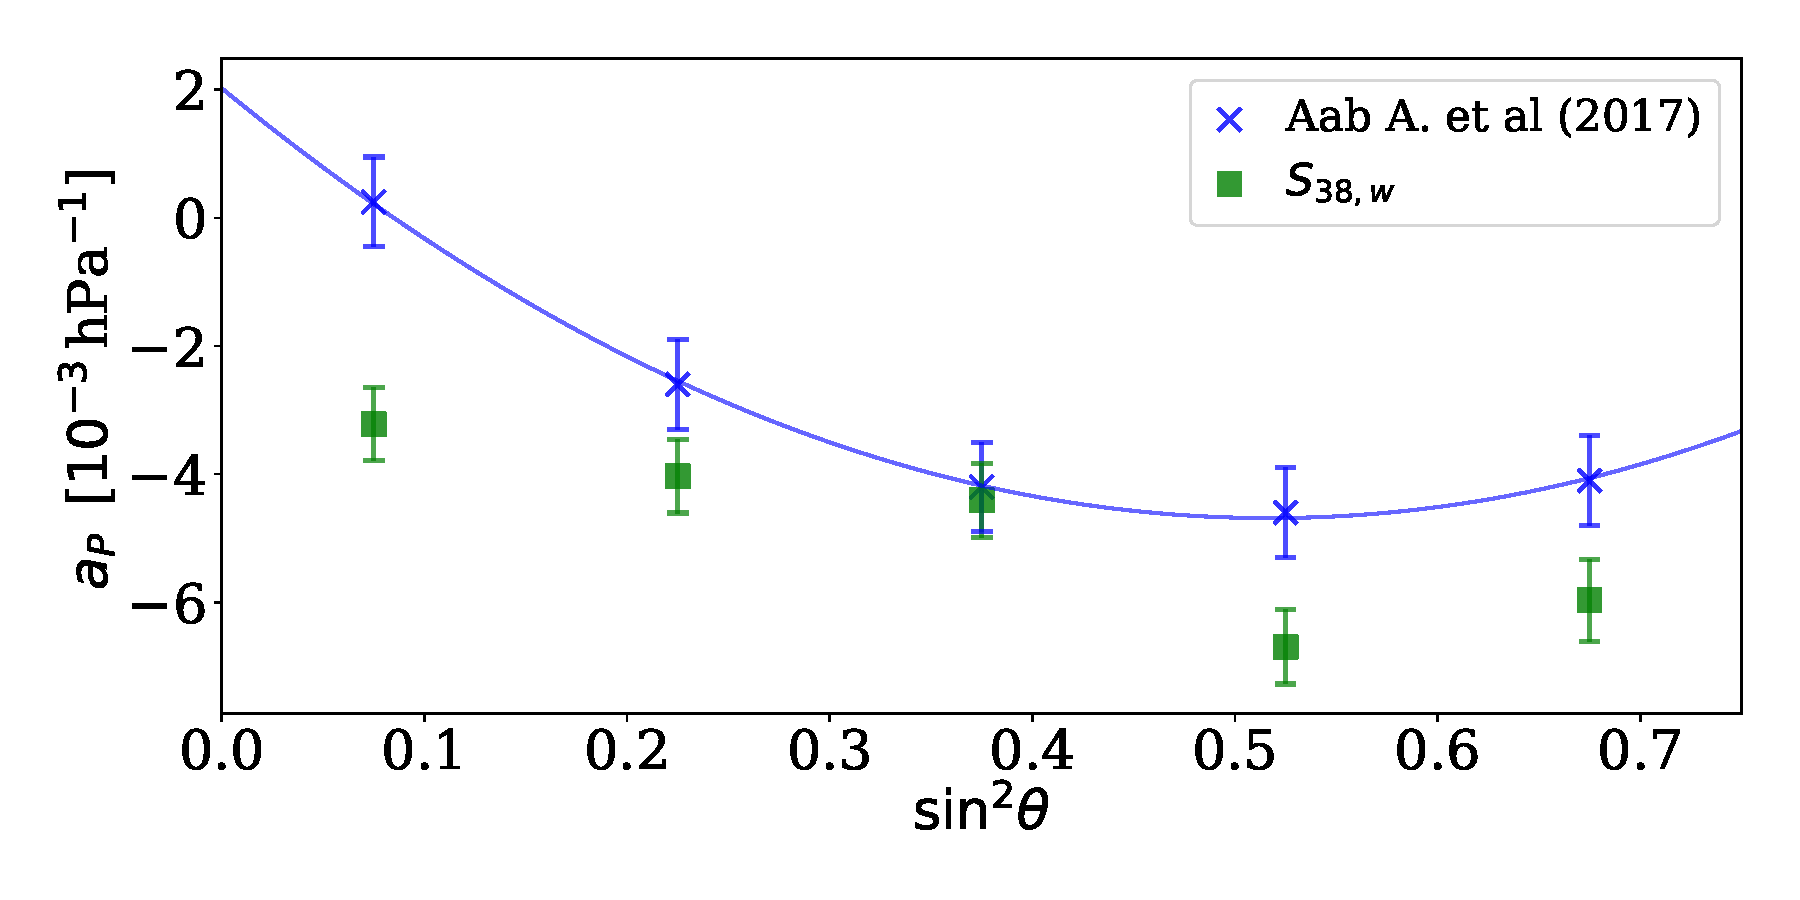
\includegraphics[width=\linewidth]{Graphs/params/ap_AllTriggers.pdf}
        %   \caption{Parámetro $a_P$ }
        %   \end{subfigure}\\
        %   \begin{subfigure}[b]{0.75\textwidth}
        %   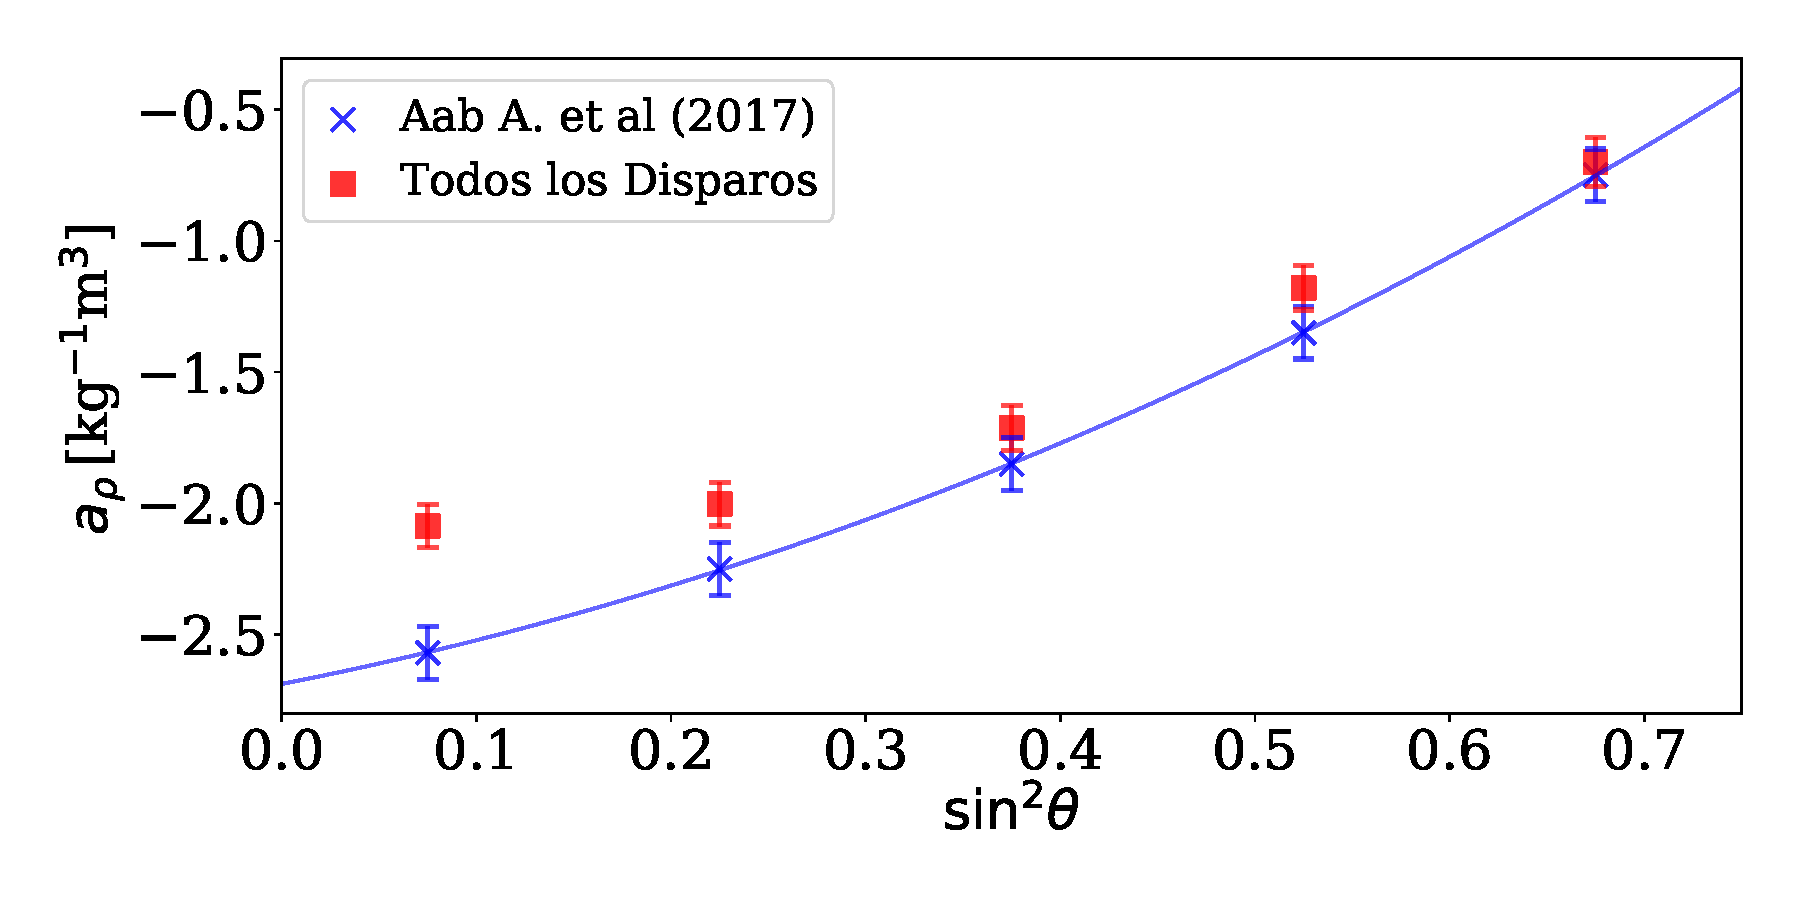
\includegraphics[width=\linewidth]{Graphs/params/arho_AllTriggers.pdf}
        %   \caption{Parámetro $a_{\rho}$ }
        %   \end{subfigure}\\
        %   \begin{subfigure}[b]{\textwidth}
        %   \centering
        %   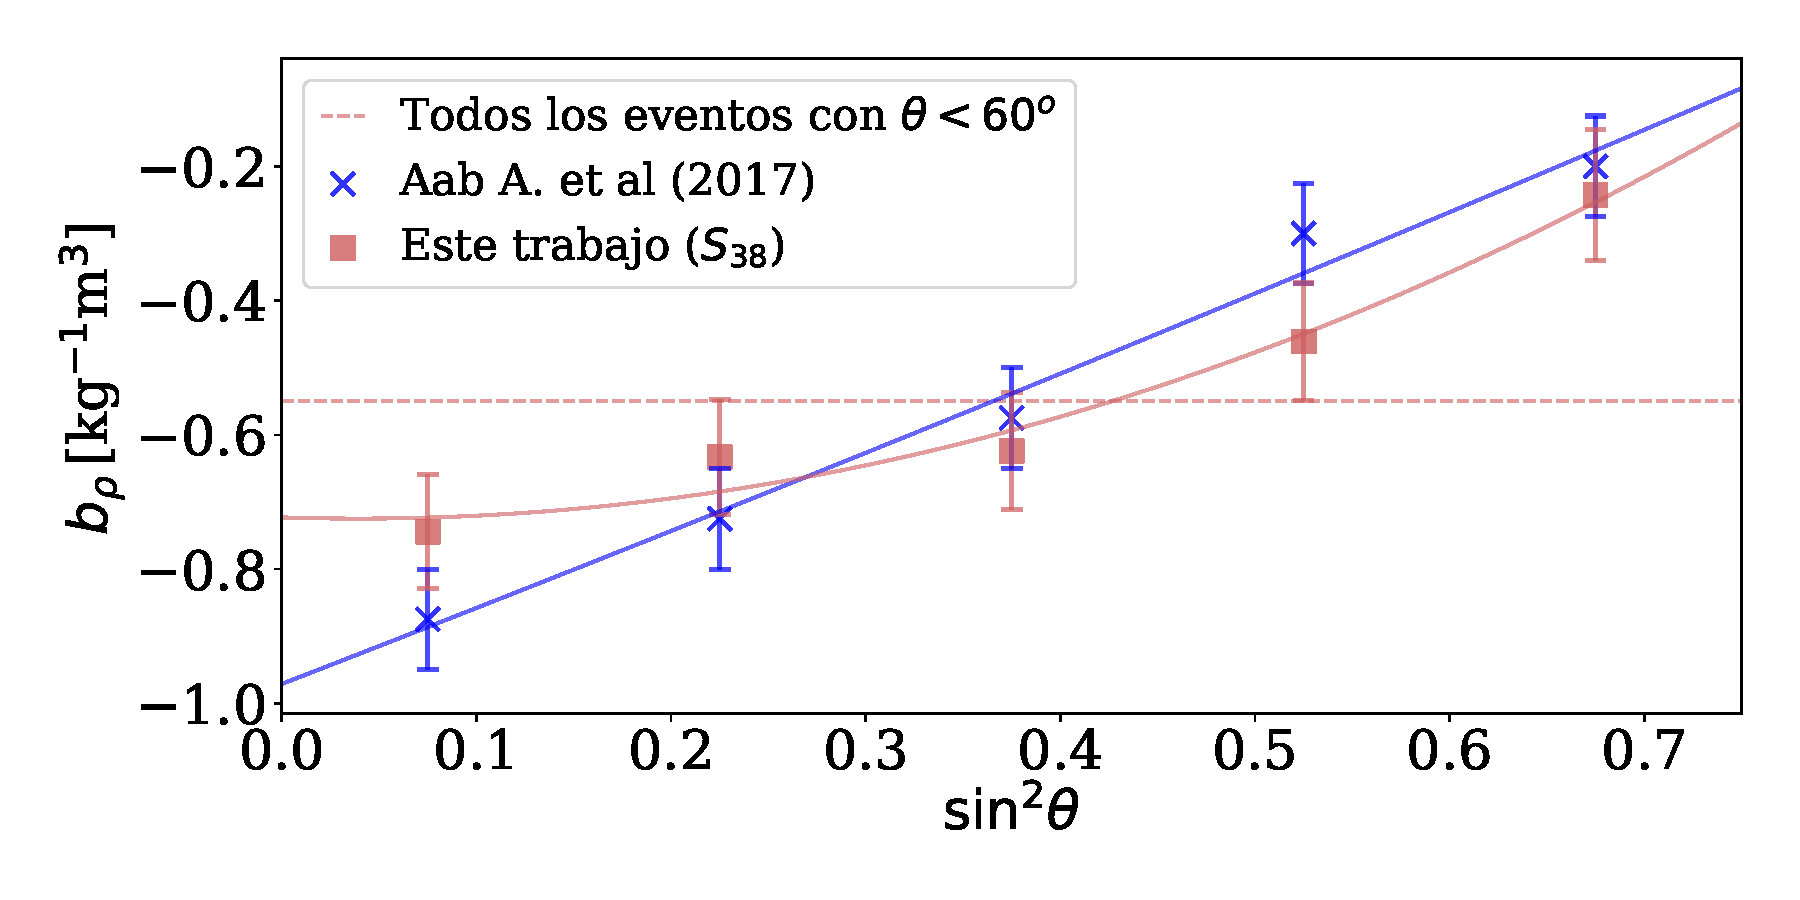
\includegraphics[width=0.75\linewidth]{Graphs/params/brho_AllTriggers.pdf}
        %   \caption{Parámetro  $b_\rho$   }
        %   \end{subfigure}
        %   \caption{Parámetros de la modulación del clima considerando los datos para Todos los Disparos del archivo 2017 y 2020. Los mismos se comparan con los coeficientes utilizados por la Colaboración.}
        % \end{figure}

%       ???????????Se ve que estos parámetros no son comparables. 


	
\chapter{Método Rayleigh}
	\graphicspath{{../05_MetodoRayleigh/}}
	% METODOS
El estudio de la distribución de las direcciones de arribo de los eventos es una herramienta importante para obtener información sobre el origen de los RCs . Las irregularidades sobre el flujo casi isotrópico de los RCs, en un rango de energía, pueden deberse a  zonas del espacio donde se producen más RCs que en otras, estas irregularidades se conocen como anisotropías. 

El análisis de anisotropías a grandes escalas angulares suele ser hecho sobre las irregularidades de la distribución de eventos en ascensión recta $\alpha$, ya que el arreglo principal tiene una exposición direccional en función de esta coordenada casi constante \cite{referencia_anis}.

\section{Cálculo de los coeficientes de Fourier para el análisis de anisotropía en ascensión recta}

Las anisotropías son variaciones pequeñas por lo que eliminar todo factor espurio en el análisis es importante. Para obtener la amplitud de la misma en ascensión recta, se estudia la frecuencia sidérea ($f_{sid}=366.25\,$ ciclos/año) \cite{taborda}. Los errores sistemáticos debido a la modulación de eventos por el clima u otros errores propios de la adquisición de datos, aparecen en la frecuencia solar  ($f_{sid}=365.25\,$ ciclos/año), por lo que se debe tener en consideración el análisis de esta frecuencia. La frecuencia anti-sidérea ($f_a=364.25\,$ ciclos/año) es una frecuencia que puede indicar efectos sistemáticos en la amplitud de la anisotropía en la frecuencia sidérea \cite{farley1954sidereal}. La mezcla entre modulaciones diarias y anuales induce bandas laterales ubicadas a $\pm1\,$ciclo/año con respecto a la solar \cite{taborda}. Por estos motivos se toman estas frecuencias  como referencia.

  \subsection{Variaciones relativas de los hexágonos} \label{peso_hexagonos}

Para corregir las variaciones de la exposición del observatorio, podemos definir un peso  $w_i$ por cada evento $i$, que corrige la variación  $\Delta N_{cell}(\alpha^0)$ en función de la ascensión recta del cenit del observatorio $\alpha^0$ durante el rango de tiempo estudiado. Estas variaciones pueden deberse al crecimiento del arreglo a través de los años,  por caídas en la comunicación del observatorio con los SDs u otros motivos. 

El factor $\Delta N _{cell}(\alpha^0)$ tiene en cuenta que la exposición  direccional  el observatorio no es uniforme en tiempo sidéreo.  Se obtiene sumando el número de celdas durante el periodo de medición, en cada segmento de $\alpha^0$ y luego se normaliza con el valor medio de los segmentos.

Para calcular estos pesos $w_i$, se sigue el algoritmo presentado a continuación:
     
      \begin{enumerate}
        \item Se establecen una frecuencia $f$  y un rango de tiempo a estudiar. Por ejemplo, se desea estudiar la frecuencia solar entre el 1 de Enero del 2014 a las 12:00:00 GMT y el 1 de Enero del 2020 a las 12:00:00 GMT.

        \item Cada dato del registro de hexágonos, tomado en un momento $t$ durante el rango seleccionado, se clasifica según la cantidad de horas desde un momento de referencia $t_0$. Esta referencia $t_0$ se tomará como el 1 de Enero del 2005 a las 00:00:00 GMT, o  $21\,$hs del 31 de Diciembre del 2004, según la hora local de Malargüe.

        \item Podemos asociar una coordenada angular $h$ a $t$  y $f$  utilizando la siguiente expresión:
         \begin{equation}
          h = (t-t_0) \times \frac{360^o}{24\text{hs}} \times\frac{f}{f_{Solar}} + h_0
          \label{eq:h_horas} 
        \end{equation}
        El factor $\nicefrac{f}{f_{Solar}}$ sirve para hacer un cambio de escala temporal entre los periodos de distintas frecuencias. Se usa como referencia la $f_{Solar}$ dado que las horas (solares) se basan en esta frecuencia, y el valor de $h_0=31.4971^o$ representa la ascensión recta del cenit del observatorio en el momento utilizado como referencia.
        
        \item  Para simplificar el cálculo del peso de los hexágonos, se divide los $360^o$ de la ascensión recta en $L$ segmentos de $\nicefrac{360}{L} ^o$ cada uno. Para clasificar un dato se  toma  el valor $h$  y se calcula
        \begin{equation}
          h' = h\, mod \,360 %=  h - 360\Big \lfloor \frac{h}{360} \Big \rfloor
          \label{eq:h_primado}
        \end{equation}
        donde la función $mod$ representa la función módulo que devuelve un número real positivo. Con el valor de $h'$ del dato, se asigna el mismo al segmento $k$ que le corresponde, mediante la siguiente expresión
        \begin{equation}
          k = \bigg \lceil \frac{h'}{360}\times L \bigg \rceil
        \end{equation}
        donde $\lceil a \rceil$ representa la función techo \footnote{La función techo da como resultado el número entero más próximo por exceso}. Por ejemplo, si optamos por $L=24$ y un dato en particular resulta con  $h=395\,^o$, esto implica que $h'= 35^o$ y que $k=\lceil 2.333 \rceil=3$, por lo tanto, este registro corresponde al segmento en la $3^{a}$ posición.

        \item Una vez clasificados todos los datos del registro de hexágonos, se calcula la suma  $N_{hex, j}$ de los datos que cayeron un segmento $j$ dado. Para definir la variación relativa de hexágonos  $\Delta N_{cell,k}$ de un segmento $k$ en particular, necesitamos la media de hexágonos por segmento $ \langle N \rangle$  para normalizar las variaciones.
       \begin{align}
         \langle N \rangle &= \sum^{L}_{i=1} \frac{N_{cell, i}}{L}  \qquad
         \Delta N_{cell,k} = \frac{N_{cell, k}}{\langle N \rangle}  \label{epepe}
       \end{align}

      \end{enumerate}
 En la Fig.\ref{fig:pesos_referencia} se muestran las variaciones relativas de los hexágonos en función de la ascensión recta del cenit del observatorio para las frecuencias mencionadas. Este análisis fue realizado en el marco del trabajo \cite{referencia_pesos} con eventos del periodo 2004-2017. 



       En la Fig.\ref{fig:pesos_ejemplo} se observan los valores obtenidos de $\Delta N_{cell,k}$  con el código escrito para este trabajo, en función de la ascensión recta del cenit  para $L=288$ segmentos. Se analizó el conjunto de datos  utilizado para obtener los resultados la Fig.\ref{fig:pesos_referencia}, con el fin de validar dicho código. Los datos se analizaron desde el 1 de Enero del 2004 a las 00:00:00 GMT  hasta el 1 de Enero del 2017 a las 00:00:00 GMT. Se  observa que estos los resultados obtenidos son compatibles con la Fig.\ref{fig:pesos_referencia}
      
      \begin{figure}[H]
          \centering
              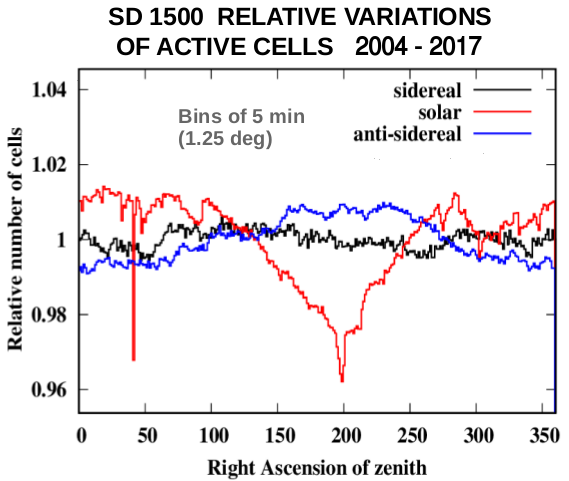
\includegraphics[width=0.5\linewidth]{pesos_referencia.png}  
              \caption{Valores de $\Delta N_{cell, k}$ en el rango 2004-2017 para distintas frecuencias obtenidas en el trabajo \cite{referencia_pesos}.}
              \label{fig:pesos_referencia}
        \end{figure}

       \begin{figure}[H]
          \centering
              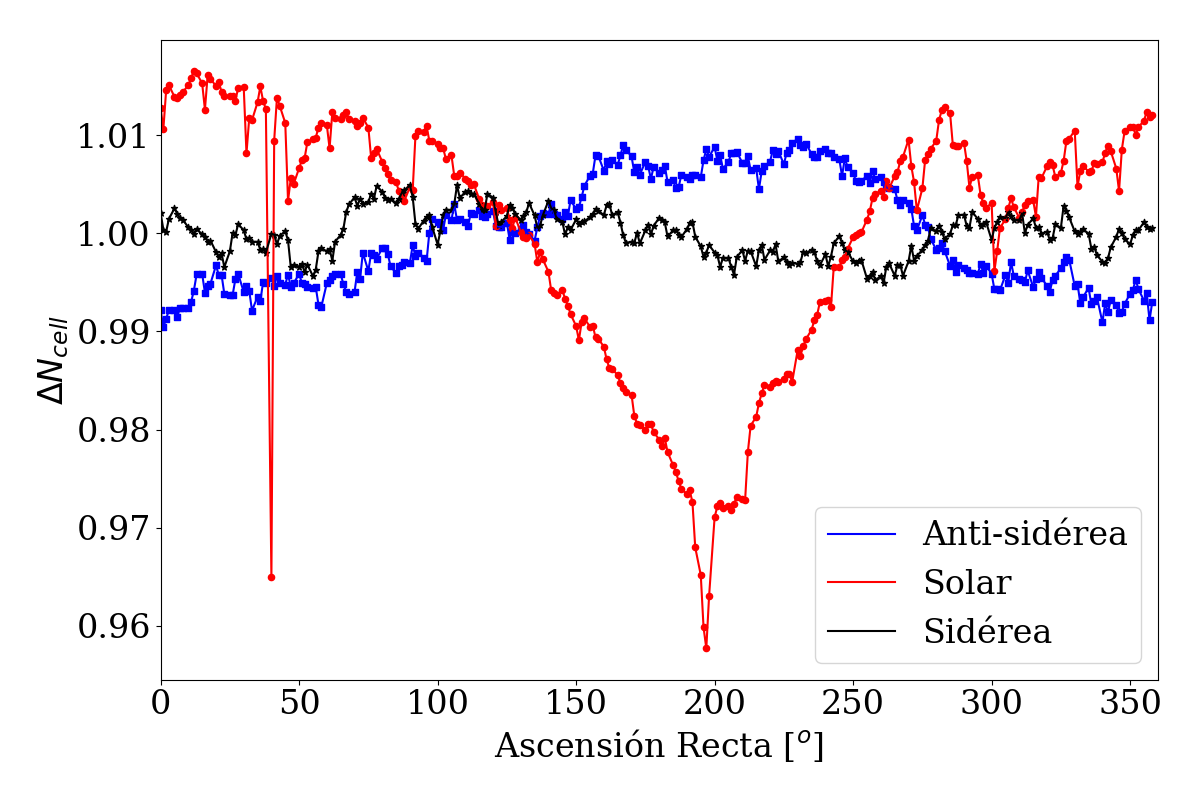
\includegraphics[width=0.75\linewidth]{weigths_2020.png}
              \caption{Valores de $\Delta N_{cell, k}$ en el rango 2004-2017 para distintas frecuencias utilizando el código escrito en este trabajo.}
              \label{fig:pesos_ejemplo}
        \end{figure}

    Para una representación fiel entre los registros de los hexágonos y los pesos de los eventos, se optó por clasificar los datos de los hexágonos en $288$ segmentos, donde cada segmento tiene un ancho de $1.25^o$. Esto es conveniente ya que la actualización del registro de hexágonos se realiza una vez  cada $5\,$min como se menciona en la sección \ref{hexagonos_rate}. Esta tasa de actualización es equivalente a decir que la adquisición se realiza cada vez que el cenit del observatorio barre  $1.25^o$ en ascensión recta sobre la esfera celeste.


  \subsection{Cálculo de Rayleigh en ascensión recta para una frecuencia dada} \label{rayleigh}

  Un procedimiento para estudiar anisotropías en la direcciones de arribos de los RCs es realizar un análisis de Fourier en ascensión recta $\alpha$. La distribución en ascensión recta $\alpha$ del flujo de RCs $I(\alpha)$ que llega al arreglo principal puede caracterizarse por las amplitudes $r_k$ y fases $\phi_k$ de su expansión en serie de Fourier al $k-$ésimo orden. 

  \begin{equation}
    I(\alpha) = I_0 \bigg ( 1+ \sum^\infty_{k=1} r_k\cos{[k(\alpha - \phi_k)]} \bigg) = I_0 \bigg ( 1+ \sum^\infty_{k=1} a_k\cos{k\alpha} +  b_k\sin{k\alpha} \bigg ) 
  \end{equation}
  donde $a_k=r_k\cos k\phi_k$ y $b_k=r_k\sin k \phi_k$, y $I_0$ es el flujo medio. La distribución $I(\alpha)$ puede obtenerse a partir de la distribución de direcciones de arribo de los eventos observados.  En este trabajo, suponiendo que existieron $N$ eventos en el rango analizado, se considera que los mismos tienen una distribución en ascensión recta del tipo $\nicefrac{dN}{d\alpha}= \sum^N_{i=1} \delta(\alpha - \alpha_i)$ \cite{taborda}. 

  Como se mencionó anteriormente, los análisis en ascensión recta están asociados a la frecuencia sidérea. Para realizar el análisis de los eventos en cualquier frecuencia arbitraria, es necesario modificar $\alpha$ por $\tilde{\alpha}$. Esta nueva variable tiene la forma como se utiliza en el trabajo \cite{taborda}:
  \begin{equation}
    \tilde{\alpha} = 2\pi f_x t_i + \alpha_i - \alpha_i^0(t_i) \label{ra_mod}
  \end{equation}
  donde $f_x$ es el frecuencia arbitraria a estudiar, $t_i$ es el momento en que ocurrió el evento y $\alpha_i^0(t_i)$ es la ascensión recta del cenit del observatorio en el momento del evento. Si la frecuencia a analizar es la sidérea, el análisis con $\alpha$ y $\tilde{\alpha}$ arrojan los mismos parámetros $r_k$ y $\phi_k$.

 Clasificando a los eventos mencionados en la sección \ref{specs} según el valor de la ascensión recta y considerando que todos los eventos tienen un peso uniforme de $w_i=1$, se dicen que los eventos fueron analizados \textit{sin pesos}, donde no consideramos la corrección de la exposición. En caso contrario, se habla de análisis \textit{con pesos} de los hexágonos  y estos pesos se calculan como se menciona en la sección anterior.

  Para realizar el análisis de frecuencias de los eventos, en el $k$-ésimo orden en la expansión de Fourier, se siguen los siguientes pasos.

        \begin{enumerate}
        \item Fijando un rango de tiempo y un rango de energía en el cual se desea estudiar la anisotropía, se establece una frecuencia en particular $f$ a analizar. Siguiendo el ejemplo de la sección anterior, se analiza la frecuencia solar entre el 1 de Enero del 2014 a las 12:00:00 GMT y 2019 hasta el 1 de Enero del 2020 a las 12:00:00 GMT.

        \item Con los eventos ya filtrados según el criterio de la sección \ref{filtro}, asigno cada evento $i$ un valor $h_i$, definida en la Ec.\ref{eq:h_horas}

        \item En caso de considerar los pesos de los hexágonos, para asignar el peso correspondiente al evento, se asocia a un segmento $k$, calculado en la sección \ref{peso_hexagonos}, mediante el valor de $h'_i$ definido en la Ec.\,\ref{eq:h_primado}. Luego, el peso asignado $w_i$  al evento $i$ es: $ w_{i}= (\Delta N_{cell,k})^{-1}$, caso contrario, se toman que todos los eventos tiene $w_i=1$.
        
        \item Para el análisis en frecuencias, a partir del valor de $h_i$ se asigna el ángulo $\tilde{\alpha}_i$ definida en la Ec.\ref{ra_mod}. La implementación en el código es de la siguiente manera: 
        \begin{equation}
         \tilde{\alpha}_i = 2\pi \frac{h_i}{24} + \alpha_i -\alpha^0_{i}
        \end{equation}
        donde $\alpha_i$  representa la ascensión recta del evento y $\alpha^0_{,i}$ la ascensión recta en el cenit del observatorio en el momento del evento. Cabe resaltar que la información de la frecuencia que se está estudiando se encuentra en el valor de $h$. Si la frecuencia a estudiar fuera la sidérea, el término $2\pi \frac{h}{24} $ seguiría el cenit del observatorio, por lo que este término sería equivalente a $\alpha^0_{i}$, por lo tanto en esta frecuencia $ \tilde{\alpha}_i =\alpha_i$ como es de esperarse. 
        
        \item Para calcular los coeficientes de Fourier del k-ésimo armónico $a_k$ y $b_k$, se siguen los siguiente pasos:
        \begin{enumerate}
          \item Por cada evento  $i$ se calculan los siguientes valores:
          \begin{equation}
             a_{ik}' = {w_i}\cos k\tilde{\alpha}_i \qquad
             b_{ik}' = {w_i}\sin k\tilde{\alpha}_i
         \end{equation}
         \item Una vez que se obtuvieron los valores de $a_{ik}'$ y $b_{ik}'$ para todos los eventos en el rango de tiempo estudiado, se calculan los coeficientes definidos en el trabajo \cite{analisis_fourier} mediante:
         \begin{alignat}{3}
          \mathcal{N} &= \sum^{Eventos}_i w_i \qquad
            a_k = \frac{2}{\mathcal{N}} \sum^{Eventos}_i a_{ik}' \qquad
            b_k = \frac{2}{\mathcal{N}} \sum^{Eventos}_i b_{ik}'  
         \end{alignat}
        \end{enumerate}
        \item Con los coeficientes es posible calcular la amplitud de la frecuencia estudiada $\tilde{r}$ y la fase $\phi$. Otros parámetros calculados para el análisis son la probabilidad $P(\tilde{r})$  y $r_{99}$. 
        \begin{alignat}{3}
            \tilde{r}_k &= \sqrt{a_k^2 +b_k^2}                       \qquad &&   \phi_k&&= \frac{1}{k}\arctan\frac{a_k}{b_k}\\
          P(\tilde{r}_k)&= \exp(-\mathcal{N}\frac{\tilde{r}_k^2}{4})\qquad &&   r_{99}&&= \sqrt{\frac{-4\log(0.01)}{\mathcal{N}}}
        \end{alignat}
        Cabe resaltar que el $r_{99}$ depende solamente de los pesos de los eventos que se está estudiando. La interpretación  de este valor es cual es la probabilidad de tener una amplitud mayor como una fluctuación de una distribución isotrópica sea del $1$\%
        %., y el valor de amplitud $r_{99}$ para que dicha probabilidad sea del $1$\%.
      \end{enumerate}

    Una forma de validar el código para el análisis de anisotropía es comparar los resultados del código con los obtenidos en otros trabajos \cite{taborda}. En la Fig.\ref{fig:sin_pesos_referencia} se muestra el análisis hecho sobre el mismo conjunto de eventos. Estos eventos fueron adquiridos con el disparo estándar desde el 1 de Enero del 2004 a las 00:00:00 GMT  hasta el 1 de Enero del 2017 a las 00:00:00 GMT. Se consideraron los eventos por encima de $8\,$EeV que además cumplan las condiciones dadas en la sección \ref{filtro}.  En esta figura que los resultados obtenidos en \cite{taborda} y con el código utilizado por este trabajo son indistinguibles. 

      \begin{figure}[H]
        \centering
        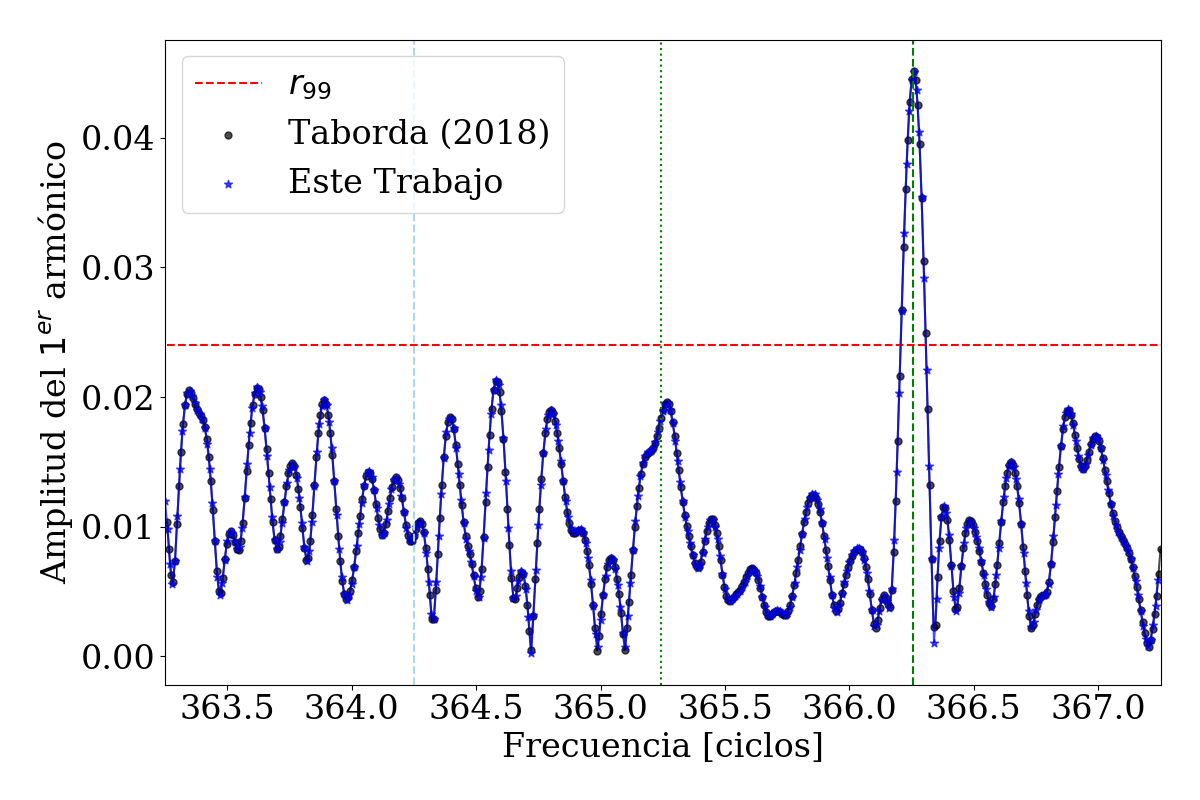
\includegraphics[width=0.75\linewidth]{sin_pesos_referencia_8_EeV.png}
        \caption{Comparación entre los análisis de anisotropía hechos para el mismo conjunto de datos, con el código de \cite{taborda} y con el código escrito para este trabajo.}
        \label{fig:sin_pesos_referencia}
      \end{figure}


\chapter{Método East-West}
	\graphicspath{{../EW/}}
	

El método de Rayleigh se basa ajustar el flujo de CRs en función de la ascensión recta mediante una función armónica. El mismo permite calcular la amplitud de la anisotropía para distintos armónicos, su fase y la probabilidad de detectar la misma señal debido a fluctuaciones de una distribución isótropa de RCs. 

La dificultad en utilizar el método Rayleigh recae en procesamiento de los datos: efectos del clima,  variaciones en el área del Observatorio, y la sensibilidad de los instrumentos deben tenerse en cuenta.  Los efectos mencionados deben ser corregidos de la señal medida de los eventos, ya que los mismos inducen modulaciones espurias en el análisis.

En el método East - West consiste en el ajuste de una función armónica a la diferencia entre los flujos de eventos provenientes del Este y del Oeste. Si se consideran que las modulaciones espurias producidas por los efectos atmosféricos y sistemáticos son las mismas en ambas direcciones, la diferencia de flujos remueve estos efectos sin realizar correcciones adicionales. Una desventaja de este método es que su sensibilidad es menor que el método de Rayleigh \cite{taborda}.


\section{Descripción de una anisotropía dipolar}
Las anisotropías en las direcciones de llegada de los RCs indican que ciertas zonas del cielo tienen una variación significativa con respecto a la media de flujo de RCs. Esta anisotropía puede describirse mediante funciones armónicas, la más sencilla es la anisotropía dipolar es una aproximación a primer orden.

Una anisotropía dipolar se puede describir de la siguiente forma:
\begin{equation}
    \Phi(\hat{\bf{u}}) = \Phi_0(1+\bf{d}\cdot\hat{\bf{u}})
    \label{eq:dipolo_general}
\end{equation}
\noindent donde $\Phi_0$ es el flujo medio de eventos, $\hat{\bf{u}}$ es un versor que apunta a la dirección a estudiar, y $\bf{d}$ es el vector con módulo igual a la amplitud del dipolo y con dirección al eje del mismo. Tomando coordenadas ecuatoriales \footnote{Referencia al apéndice de ecuatoriales}, la dirección de $\bf{d}$ es $(\alpha_d, \delta_d$) y  de $\hat{\bf{u}}$ es $(\alpha, \delta)$, por lo tanto  el producto escalar  entre estos vectores se puede escribir de la siguiente manera \footnote{Falta mencionar el producto de versor de esta representación para decir sale de acá. Eso va a estar en el apéndice porque el cálculo me  sale fácil poniendo  todo en cartesianas.)}:
\begin{equation}
    \textbf{d}\cdot\hat{\bf{u}}= d (\cos\delta_d \cos\delta \cos(\alpha - \alpha_d) + \sin\delta_d  \sin\delta)
    \label{eq:product_ud}
\end{equation}


Otro aspecto importante de la representación del dipolo en coordenadas ecuatoriales, es que la proyección de la amplitud del dipolo sobre el plano ecuatorial se puede aproximar de la siguiente manera:
\begin{equation}
    r_1 \simeq d_\perp \langle \cos\delta \rangle
    \label{eq:fourier_perp}
\end{equation}
donde $r_1$ es la amplitud de la aproximación a primer orden en Fourier, y $\langle \cos\delta \rangle$ es el valor medio de $\cos\delta $ de los eventos utilizados para realizar la aproximación mencionada.

\subsection{Representación en coordenadas locales de la anisotropía dipolar}
Podemos reescribir el producto escalar entre dipolo $\textbf{d}$ y el versor $\hat{u}$ apunta en la dirección cualquiera mediante las coordenadas locales $\theta$ y $\phi$ \footnote{Referencia locales apéndice}.
\begin{align}
    \textbf{d} &=  d_x(\alpha^0)\hat{x} +  d_y(\alpha^0)\hat{y}+ d_z(\alpha^0)\hat{z} \\
    \hat{\bf{u}} &=\sin\theta \cos\phi \hat{x} + \sin\theta \sin\phi \hat{y} + \cos\theta\hat{z}\\
    \textbf{d}\cdot\hat{\bf{u}} &= d_x(\alpha^0)\sin\theta \cos\phi
    + d_y(\alpha^0) \sin\theta \sin\phi  
     + d_z(\alpha^0)\cos\theta \label{eq:dot-prod-local}
\end{align}
donde los versores $\hat{x}$, $\hat{y}$ y $\hat{z}$ apuntan a la dirección Este, Norte  y  del cenit respectivamente. 

El dipolo está fijo en el cielo pero visto desde las coordenadas locales para poder trabajar con $\theta$ y $\phi$, sus proyecciones  proyecciones $d_x$, $d_y$ y $d_z$  tienen una dependencia con la ascensión recta  $\alpha^0$ y declinación $\delta_0$ del cenit. 

\section{Descripción formal del método East-West}

    \subsection{Flujo de eventos del Este y Oeste}
    El flujo de eventos observado $I^{obs}(\alpha^0)$ para la ascensión recta del cenit $\alpha^0$ entre los ángulos azimutales $\phi_1$ y $\phi_2$ puede calcularse mediante el flujo total de RCs $\Phi(\theta, \phi, \alpha^0)$ (expresado en coordenadas locales) como
    \begin{equation}
        I^{obs}(\alpha^0) = \int_{\phi_1}^{\phi_2} d\phi \int_{0}^{\theta_{max}} d\theta \sin\theta \tilde{\omega}(\theta, \alpha^0) \Phi(\theta, \phi, \alpha^0),
        \label{eq:rate_general}
    \end{equation}
    \noindent  donde  el término $\tilde{\omega}(\theta, \alpha^0)$ representa la exposición del Observatorio. Este término también incluye los efectos sistemáticos y atmosféricos, como la variación de los hexágonos del arreglo y las correcciones de la modulación del clima, mediante  su dependencia con $\alpha^0$.

    Para calcular los flujos de eventos del Este y Oeste, $I^{obs}_E$ y $I_O^{obs}$ respectivamente, se integra la Ec.\ref{eq:rate_general} en los siguientes  rangos: para el Este: entre $\phi_1=\nicefrac{-\pi}{2}$ y $\phi_2=\nicefrac{\pi}{2}$ y para el Oeste: entre $\phi_1=\nicefrac{\pi}{2}$ y $\phi_2=\nicefrac{3\pi}{2}$.

    \subsection{Aproximaciones del método}
    Se considera que pueden  desacoplarse de las variables $\theta$ y $\alpha^0$, por lo tanto, podemos expresar $\tilde{\omega}$ de la siguiente manera:
    \begin{equation}
        \tilde{\omega}(\theta, \alpha^0) = \omega(\theta)F(\alpha^0)
    \end{equation}    
    
    A su vez, consideremos que las amplitudes de las variaciones asociadas a $\tilde{\omega}$ son pequeñas con respecto al valor medio, por lo que se puede tomar la expansión en primer orden de la función $F(\alpha^0)$:
    \begin{equation}
        \tilde{\omega}(\theta, \alpha^0) = \omega(\theta)\big(1 + \eta(\alpha^0) \big)
        \label{eq:omega_expandido}
    \end{equation}
    \subsection{Cálculo de la diferencia de flujos}
  
    Teniendo en cuenta la Ec.\ref{eq:omega_expandido} y \ref{eq:dipolo_general}, se tiene la siguiente expresión:
    \begin{align}
        I^{obs}(\alpha^0) &= \int_{\phi_1}^{\phi_2} d\phi \int_{0}^{\theta_{max}} d\theta  \sin\theta \omega(\theta)\big(1 + \eta(\alpha^0) \big) \Phi_0 ( 1 +  \textbf{d}\cdot\hat{\bf{u}}) \label{eq:I-obs}
    \end{align}
    donde la primera parte  de la igualdad  puede simplificarse con una definición apropiada  \footnote{ $
        \text{Por simplicidad, definimos la siguiente expresión: }
      \overline{f(\theta)} = \int_{0}^{\theta_{max}} d\theta \sin\theta \omega(\theta) f(\theta)
      \label{eq:media_angular}
  $
  \noindent, donde $\overline{f(\theta)}$ es la media de la función $f(\theta)$ sobre el ángulo cenital pesado por la exposición del Observatorio $\omega(\theta)$, hasta  un ángulo máximo de $\theta_{max}$. En este trabajo se centra en eventos hasta 2 EeV, por lo que $\theta_{max}=60^o$ para los datos del Observatorio.}. Además dado que la integral sobre $\phi$ tiene el mismo valor para el Este y Oeste, se  obtiene que la primera parte se puede escribir de la siguiente forma
    \begin{align*}
        &\int_{\phi_1}^{\phi_2} d\phi \int_{0}^{\theta_{max}} d\theta \sin\theta \omega(\theta)\big(1 + \eta(\alpha^0) \big) \Phi_0 
        = \Phi_0 (1+ \eta(\alpha^0)) \overline{1}. 
    \end{align*}
    Trabajando con la segunda parte de la expresión \ref{eq:I-obs}, si  consideramos la expresión \ref{eq:dot-prod-local} del producto escalar $\textbf{d}\cdot\hat{\bf{u}}$ en coordenadas locales, e integramos el ángulo  $\phi$ entre $[\nicefrac{-\pi}{2}, \nicefrac{\pi}{2}]$ o $[\nicefrac{\pi}{2}, \nicefrac{3\pi}{2}]$, se obtiene que:

    \begin{align}
        &\int_{\phi_1}^{\phi_2} d\phi \int_{0}^{\theta_{max}} d\theta \sin\theta \omega(\theta)\big(1 + \eta(\alpha^0) \big) \Phi_0 \textbf{d}\cdot\hat{\bf{u}}=\\
        &=\Phi_0 (1+ \eta(\alpha^0)) \int_{0}^{\theta_{max}}  d\theta (\pm 2d_x(\alpha^0)\sin\theta 
        + \pi d_z(\alpha^0)\cos\theta) \label{segundo_term}
    \end{align}
    \noindent donde $+2$ corresponde al Este y $-2$ al Oeste. No hay una dependencia con la proyección del dipolo $d_y$ porque en la integral aparece el término $\int_{\phi_1}^{\phi_2}\, d\phi\, d_y(\alpha^0) \sin\theta \sin\phi $, que se anula al integrar sobre el Este y Oeste.

     Usando la definición dada en la nota \ref{eq:media_angular} y la expresión \ref{segundo_term}, podemos reescribir la expresión \ref{eq:I-obs} y los flujos para el Este y el Oeste como:
    \begin{align*}
    I^{obs}_E&= \Phi_0 (1+ \eta(\alpha^0)) \Big( \pi\overline{1} + 2d_x(\alpha^0)\overline{\sin\theta} + \pi d_z(\alpha^0)\overline{\cos\theta}  \Big) \\
        I^{obs}_O&= \Phi_0 (1+ \eta(\alpha^0)) \Big( \pi \overline{1} - 2d_x(\alpha^0)\overline{\sin\theta}   + \pi d_z(\alpha^0)\overline{\cos\theta} \Big) \\
        I^{obs}&= \Phi_0 (1+ \eta(\alpha^0)) \Big( 2\pi\overline{1} +\pi d_z(\alpha^0)\overline{\cos\theta}  \Big)
    \end{align*}
    Ya que se busca calcular la diferencia entre los flujos provenientes del Este y del Oeste, $I^{obs}_E $ y $  I^{obs}_O $ respectivamente, esta resta queda como:
    \begin{equation*}
        I^{obs}_E -  I^{obs}_O = 4 \Phi_0 (1+ \eta(\alpha^0)) \,  d_x(\alpha^0)\overline{\sin\theta}
    \end{equation*}

    Para obtener las componentes del vector $\bf{d}$, tenemos que considerar que las mismas están en el plano x-z. Para hacer esto, consideremos a los versores $\hat{\bf{u}}_x$ y $\hat{\bf{u}}_z$ que apuntan al cenit y al Este respectivamente. Podemos obtener las proyecciones con un producto escalar con los versores en las direcciones de interés:
    \begin{equation}
        d_x(\alpha^0) \hat{x} =  (\textbf{d}\cdot\hat{\bf{u}}_x)\hat{\bf{u}}_x \rightarrow d_x(\alpha^0) = \textbf{d}\cdot\hat{\bf{u}}_x,
    \end{equation}
    donde estos versores en coordenadas ecuatoriales se escriben como:
    $\hat{\bf{u}}_z = (\alpha^0,\delta_0 )$ y $ \hat{\bf{u}}_x = (\alpha^0 + \frac{\pi}{2},0)$ \footnote{Se suma  $\frac{\pi}{2}$ para apuntar al Este, cuando el versor recorre $\nicefrac{\pi}{2}$ en ascensión recta, llega al plano del ecuador que tiene declinación $0$.}.

    Usando la expresión \ref{eq:product_ud} para el producto escalar en coordenadas ecuatoriales, se obtienen las componentes:
    \begin{align*}
        d_z=\textbf{d}\cdot\hat{\bf{u}}_z &= d (\cos\delta_d \cos\delta_0 \cos(\alpha^0 - \alpha_d) + \sin\delta_d  \sin\delta_0)\\
        d_x=\textbf{d}\cdot\hat{\bf{u}}_x &= d (\cos\delta_d \cos(\alpha^0 +\frac{\pi}{2} - \alpha_d) 
        = -d\cos\delta_d \sin(\alpha^0  - \alpha_d)
    \end{align*}
    
     Entonces la diferencia entre flujos queda como:
    \begin{equation}
        I^{obs}_E -  I^{obs}_O =-4d \Phi_0 (1+ \eta(\alpha^0)) \cos\delta_d \sin(\alpha^0  - \alpha_d)\overline{\sin\theta}
        \label{resta}
    \end{equation}

    Esta diferencia se debe relacionar con la variación del flujo verdadero $I(\alpha^0)$, es decir el flujo que se observaría si no existieran variaciones temporales en ascensión recta en la exposición, que implicaría $\eta(\alpha^0)=0$. 

    La variación del flujo verdadero en ascensión recta provee información sobre la componente $d_z$ del dipolo. 
    \begin{align}
        \dv{I(\alpha^0)}{\alpha^0}  & = 2\pi\Phi_0 \overline{\cos\theta} \dv{\,d_z(\alpha^0) }{\alpha^0}\\ 
        \dv{I(\alpha^0)}{\alpha^0} &= -2d\pi\Phi_0 \overline{\cos\theta}\cos\delta_d \cos\delta_0 \sin(\alpha^0 - \alpha_d) \label{total_flux}
    \end{align}

    Para llegar a la expresión \ref{resta}, hicimos la expansión hasta el primer orden de $\tilde{\omega}(\theta, \alpha^0)$ y de $\bf\Phi(\alpha, \delta)$, por lo tanto, para ser consistentes en el orden de aproximación, se desprecia el término de segundo orden de la expresión \ref{resta} que es proporcional de $\eta \cdot d$ y la expresión \ref{resta} queda:
        \begin{equation}
            I^{obs}_E -  I^{obs}_O \approx -4d \Phi_0 \cos\delta_d \sin(\alpha^0  - \alpha_d)\overline{\sin\theta}
            \label{resta_final}
        \end{equation}

    Considerando las expresiones \ref{total_flux} y \ref{resta_final}, se tiene una relación entre el flujo observado por el Observatorio  y el flujo real de RCs \footnote{
    $
        \text{Se usa la expresión:  }
        \langle f(\theta) \rangle = \frac{\overline{f(\theta)}}{\overline{1}} = \displaystyle\frac{\int_{0}^{\theta_{max}} d \theta \sin\theta \omega(\theta) f(\theta) }{\int_{0}^{\theta_{max}} d \theta \sin\theta \omega(\theta)} 
    $,  
    que es equivalente a hacer la media ponderada de todos los datos de $f(\theta)$.} %Como consideramos una expansión de $\omega(\theta)$ }:
    \begin{equation}
        I^{obs}_E -  I^{obs}_O \approx  \frac{2}{\pi \cos \delta_0} \frac{\langle\sin\theta \rangle}{\langle\cos\theta \rangle}\dv{I(\alpha^0)}{\alpha^0} 
        \label{eq:final}
    \end{equation}
   

\section{Estimación de la componente ecuatorial del dipolo mediante el análisis del  primer armónico}


El objetivo del método  East - West es estimar la modulación dipolar de  $I(\alpha^0)$ a partir de la diferencia $I^{obs}_E -  I^{obs}_O$ mediante un análisis similar al método de  Rayleigh, salvo modificaciones para tener en cuenta la dirección de los eventos. 
\begin{equation}
    I^{obs}_E -  I^{obs}_O = \frac{N}{2\pi} r_{EW} \cos(\alpha^0 -  \phi_{EW}) \label{eq:ray_ew_like}
\end{equation}
La amplitud $r_{EW}$ y fase $\phi_{EW}$ obtenidas por el Método  East - West no es la amplitud del dípolo físico aunque está relacionada con la misma. 


Esta relación puede obtenerse reescribiendo la expresión \ref{eq:final}, teniendo en cuenta la proyección del dípolo físico sobre el ecuador $d_{\perp}= d\cos\delta_0$, la expresión  \ref{resta_final} y que $N \simeq 4\pi^2 \Phi_0 \overline{1} $ \footnote{Porque es la integral con respecto a los dos ángulos, $\theta$ y $\phi$}:
\begin{align}
    I^{obs}_E -  I^{obs}_O \approx -4 d_\perp \frac{N}{ 4\pi^2\overline{1}} \sin(\alpha^0  - \alpha_d)\overline{\sin\theta} \frac{\overline{1}}{\overline{1}}\\
    I^{obs}_E -  I^{obs}_O \approx -4 d_\perp \frac{N}{ 4\pi^2} \sin(\alpha^0  - \alpha_d)\langle\sin\theta \rangle\\
    I^{obs}_E -  I^{obs}_O \approx -\frac{N}{2\pi} d_\perp \frac{2\langle\sin\theta \rangle }{\pi}\sin(\alpha^0  - \alpha_d) \label{ultima_ew_ray}
\end{align}


Comparando las expresiones \ref{eq:ray_ew_like} y \ref{ultima_ew_ray} y considerando la ecuación \ref{eq:fourier_perp}, se puede inferir que las relaciones entre la amplitud y fase obtenidas mediante EW y el dipolo físico son las siguientes:

\begin{tabular}{@{}p{.4\linewidth}@{}p{.5\linewidth}@{}}
    \begin{align}
        d_{\perp} = \frac{2\langle\sin\theta \rangle}{\pi} r_{EW} \label{dperp} \\
        r_1   =\frac{\pi}{2} \frac{\langle\cos\delta \rangle}{\langle\sin\theta \rangle} r_{EW} \label{r_fisico}  \\
        \alpha_d = \phi_{EW} + \frac{\pi}{2} \label{phase_fisico}
    \end{align}
    &    \begin{align}
        \sigma_{x,y} = \frac{\pi}{2\langle\sin\theta \rangle} \sqrt{\frac{2}{\mathcal{N}}}\\
        \sigma   = \frac{\pi \langle\cos\delta \rangle}{2\langle\sin\theta \rangle} \sqrt{\frac{2}{\mathcal{N}}}
    \end{align}
  \end{tabular}

Como en el caso del análisis de Rayleigh, la probabilidad de obtener una amplitud mayor o igual a que $r_{EW}$ a partir de una distribución isótropa es una distribución acumulada de Rayleigh:
\begin{equation}
    P(\geq r_{EW}) = \exp \Big(-\frac{N}{4}r^2_{EW}\Big) \label{p99}
\end{equation}

\subsection{Cálculo  de la amplitud del dipolo para los eventos de Todos los Disparos}

\begin{enumerate}
    \item Definimos el rango de tiempo a estudiar, para los resultados para Todos los Disparos se utilizaron los límites: 1 de Enero del 2014 hasta el 1 de Enero del 2020.
    \item Se recorre cada evento que cumpla con las siguientes características:
     \begin{itemize}
        \item Pertenezca el rango de energía a estudiar
        \item Sea un evento 6T5 con ángulo cenital menor a $60^o$
        \item Se haya registrado en el rango de tiempo seleccionado
    \end{itemize}
    En cada evento se calcula los siguientes valores:
    \begin{align}
        a_i' = \cos(X_i - \beta) \qquad
        b_i' = \sin(X_i - \beta)
    \end{align}
    el valor de $X_i$ depende la frecuencia a estudiar, la misma es igual a la ascensión recta del cenit $\alpha^0_i$ al momento del evento  si se estudia la frecuencia sidérea, en cambio para la frecuencia solar es igual al equivalente en grados de la hora local de Malargüe. El valor de $\beta$ es depende si el evento provino del Este donde $\beta=180^o$ o $\beta=0$ caso contrario.
    
    \item Una vez corridos todos los  eventos se calculan los parámetros:
    \begin{align*}
        a_{EW} &= \frac{2}{N} \sum^N_{i=1}a_i' =\frac{2}{N} \sum^N_{i=1} \cos(X_i - \beta_i)\\
        b_{EW} &= \frac{2}{N} \sum^N_{i=1}b_i' =\frac{2}{N} \sum^N_{i=1} \sin(X_i - \beta_i)
    \end{align*}
    donde N indica la cantidad eventos considerados. La cantidad de eventos por rango de energía se muestran en la tabla \ref{tab:}.

    Con esto puedo calcular la amplitud asociada al análisis $r_{EW}$ y la fase $\phi_{EW}$:
    \begin{align*}
        r_{EW} = \sqrt{a_{EW}^2 + b_{EW}^2}\\
        \phi_{EW} = \tan^{-1}(\nicefrac{b_{EW}}{a_{EW}})
    \end{align*}

    Estos valores se traducen a los valores de amplitud $r$, $d_\perp$ y fase $\phi$ del dipolo físico mediante las expresiones \ref{dperp}, \ref{r_fisico} y \ref{phase_fisico}.   Los valores $\langle\cos\delta \rangle$ y $\langle\sin\delta \rangle$ son los valores medios de estas variables en los años estudiados. 

    \item Se calcula la amplitud límite $r_{99}$ y la probabilidad  $P(r_{EW})$ utilizando la expresión \ref{p99}:
    \begin{align*}
        r_{99} &= \frac{\pi}{2} \frac{\langle\cos\delta \rangle}{\langle\sin\theta \rangle}\sqrt{\frac{4}{N}\ln(100)}\\
        d_{\perp,99} &= \frac{r_{99}}{\langle\cos\delta \rangle}    
    \end{align*}

    \item Se calculan los límites de confianza de las variables $r$,$\phi$ y $d_\perp$ mediante los densidad de probabilidad de la amplitud y fase. Las mismas se describen en el capítulo \ref{PDFs}.


\end{enumerate}


Por último, estos resultados se comparan con los valores obtenidos con el método EW en el trabajo \cite{Aab_2020} en frecuencia sidérea, aplicado al conjunto de eventos del disparo estándar registrados entre el 1 de Enero del 2004 y el 1 de Agosto del 2018. 


\subsubsection{Cálculo para frecuencias  arbitrarias}

Cambiamos las variable de la ascensión recta del cenit $\alpha^0$ por
\begin{equation}
    \tilde{\alpha} = 2\pi f_x t_i  \label{ra_arb}
  \end{equation}
donde $f_x$ es la frecuencia arbitraria a estudiar y $t_i$ es el momento donde ocurre el evento a estudiar. Luego se realizan el mismo procedimiento que lo anterior para calcular el valor de la amplitud $r$.

En la siguiente sección se verifica que se obtiene los mismo resultados con esta variable general que con el valor de $\alpha^0$ para la frecuencia sidérea.

\section{Verificación del código}

\subsection{Comparación con el trabajo \cite{Aab_2020} de la colaboración}
Se verificó el código escrito en este trabajo de la siguiente manera:

\begin{enumerate}
    \item El conjunto de eventos del disparo estándar registrados entre el 1 de Enero del 2004 y el 1 de Agosto del 2018 fue analizado en el trabajo \cite{Aab_2020}.
    \item Utilizando el código y los datos de los eventos del paper \cite{Aab_2020}, obtenidos de la página del \emph{Publications Committee} de la colaboración Auger, se replicaron los datos del paper. 
    \item Luego utilizando el código escrito para este trabajo, se realizó el análisis de EW con los datos del trabajo \cite{Aab_2020}. 
    \item Finalmente se verificó que los valores obtenidos en los item 2 y 3, con  ambos códigos, sean el mismo.
\end{enumerate}

\subsection{Tabla comparando con la variable $\tilde{\alpha}$ con la ascensión recta del cenit }

Para verificar que la variable de la Ec.\ref{ra_arb} es útil para estudiar otras frecuencias, en la Tabla~\ref{tab:comp_vars} se comparan los resultados de la referencia para el rango $0.25-0.5$ EeV, los obtenidos usando la ascensión recta del cenit y los valores obtenidos con la Ec.\ref{ra_arb} en el mismo rango de energía. Se observan que los valores son comparables entre sí.

(FALTA ACTUALIZAR LA TABLA)
\begin{table}[H]
    \begin{small}
        \begin{center}
            \begin{tabular}[c]{l|l|l|l}
                                    & \cite{Aab_2020} & $\alpha^0$   & $\alpha=2\pi f_xt_i$   \\ 
                Frecuencia:         & 366.25          &  366.25      &  366.25            \\
                $d_\perp$[\%]:      & 0.60            &  0.60        &  0.60              \\
                $\sigma_{x,y}$[\%]  & 0.48            &  0.48        &  0.48              \\ 
                Probabilidad:       & 0.45            &  0.45        &  0.45              \\
                Fase[$^o$]:         & 225$\pm$64\cite{discrepancia} & 225$\pm$45   &  227$\pm$45          \\
                $r_{99}$[\%]:       & 1.5             &  1.5       &  1.5             \\
                $d_{\perp,99}$[\%]: & 1.8             &  1.8       &  1.8             \\
            \end{tabular}
        \end{center}
        \caption{Verificando la  variable $\alpha=2\pi ft$}
        \label{tab:comp_vars}
    \end{small}
\end{table}


	
\chapter{Distribución de probabilidad de la amplitud y fase del dipolo} \label{PDFs}
	\graphicspath{{../EW/}}
	
En el trabajo \cite{linsley1975fluctuation} se estudian los límites de confianza para la amplitud $r_1$ y la fase $\phi$ obtenidos mediante el análisis del primer armónico en Fourier. Las distribuciones de probabilidad describen a un conjunto de N mediciones cuya modulación en ascensión recta está caracterizada por el vector $\vec{s}$ con una dispersión $\sigma = \sqrt{\nicefrac{2}{N}}$.  Sin pérdida de generalidad, se puede restar a las mediciones la fase $\phi$ para que las mismas varíen alrededor del 0. Este vector $\vec{s}$ puede ser estimado mediante distintos métodos, en este trabajo se  utilizó como estimador el valor de la amplitud de la modulación en ascensión recta $r_1$ obtenido mediante el método de Rayleigh e East - West.

La distribución de probabilidad de la amplitud y la fase está dada por la Ec.\ref{eq:full_pdf}. Las variables $r$ y $\psi$ representan las amplitudes y fases medidas respectivamente
\begin{equation}
    p(r,\psi) =dr\,d\psi\,\frac{r}{2\pi\sigma^2}\exp{ -\frac{(r^2+s^2 - 2rs\cos\psi)}{2\sigma^2} } \label{eq:full_pdf}
\end{equation}  

\section{Distribución de probabilidad de la amplitud}

Integrando la Ec.\ref{eq:full_pdf} con respecto a $\psi$, se obtiene la función de densidad de probabilidad $p(r)$ y el nivel de confianza $CL$ entre en rango $[r_i,r_f]$:
\begin{align}
    p(r) &=\frac{r}{\sigma^2}\exp{ -\frac{(r^2+s^2)}{2\sigma^2} }K_0(\frac{rs}{\sigma^2})    \label{ec:pdf}\\
    CL_r(r_i,r_f,s) &= \int_{r_i}^{r_f} dr \, p(r)
    \label{ec:integral}
\end{align}
donde $K_0(x)$ es la función de Bessel modificada de primer orden.
Estas ecuaciones nos permiten determinar el nivel de confianza $CL$ con el cual se puede afirmar que el módulo del dipolo se encuentra entre los valores $r_i$ y $r_f$.

Se define el valor $r^{UL}$ como el límite superior donde se puede afirmar que el módulo de dipolo se encuentra en el rango $[0, r^{UL}]$ con un $99\%$ de certeza.
\begin{align}
    CL_r(0,r^{UL},s) = 0.99 = \int_{0}^{r^{UL}} dr \, p(r)
    \label{ec:r_upper_limit}
\end{align} 
% Para alcanzar un  nivel del confianza  del  CL[\%] \footnote{ Donde CL=.99 para un 99\% o CL=0.68 para un 68\%,},  se toma el valor de amplitud $r^{UL}$ y la integral de la función \ref{ec:pdf} desde 0 hasta $r^{UL}$, donde el resultado debe ser el nivel de confianza CL.
% \begin{align}
%     CL = \int_{0}^{r^{UL}} dr \frac{r}{\sigma^2}\exp{\Big( -\frac{(r^2+s^2)}{2\sigma^2} + \frac{rs}{\sigma^2}\Big)}K_0(\frac{rs}{\sigma^2})
%     \label{ec:integral}
% \end{align}

Suponiendo que mediante el análisis de un conjunto de eventos, se obtiene que $s=0.0047$ y $\sigma=0.0038$. El gráfico de la función $p(r)$ se muestra a continuación:

\begin{figure}[H]
    \begin{small}
        \begin{center}
            \includegraphics[width=0.75\textwidth]{bessel_prob_value_s_v2.pdf}
        \end{center}
        \caption{El gráfico de la densidad de probabilidad $p(r)$ de la amplitud $r$ para $s=0.0047$ y $\sigma=0.0038$ }
    \end{small}
\end{figure}

\subsection{Haciendo la cuenta de los márgenes de confianza de la amplitud}

Calculemos los márgenes de confianza para el ejemplo anterior de $s=0.0047$ y $\sigma=0.0038$. En este trabajo los márgenes que se obtuvieron nos dicen que el nivel de confianza en ese intervalo del $68.27\%$. Se toma este límite, dado que si $N>>1$, la distribución $p(r)$ tiende a una distribución normal y el nivel de confianza sería $1\sigma$.

Los pasos para el cálculo son los siguientes: 

\begin{enumerate}
    \item 
    Dado que la distribución tiene una función de bessel modificada de primer orden que diverge en el 0, se toma una aproximación a la función con los primeros 8 términos de la sucesión. Por lo que la función no es exacta y la norma difiere de $1$. 
    
    Para normalizar el área, se calcula la integral hasta $r_{max}=s +  10\sigma$, dado que está tan alejada del valor de amplitud obtenida, el nivel de confianza en $CL_r(0,r_{max},s)\simeq 1$, por lo que se  usa este valor para normalizar la Ec. \ref{ec:pdf} en el código.

    \item Una vez que se tiene la función normalizada, se calcula la integral de la ecuación \ref{ec:integral} $CL_r(0,s,s)$ en el intervalo  $[0,s]$ y se obtiene el valor de la función $p(s)=p_1$.

    % \item Si $CL_r(0,s,s)< 0.6827$:
    % \begin{enumerate}
        \item Teniendo en cuenta el valor inicial de $p_1$, se actualiza el valor  $p_2 \leftarrow p_1 - 0.01 p_1$ \label{itm:1}.
        \item Se calcula la integral entre los dos puntos con valores igual a $p_2$. 
        \item \label{itm:3} Si la integral es menor a $0.6827$, se repite el proceso desde el paso \ref{itm:1}. Caso contrario, si esta integral es mayor o igual a $0.6827$, se calculan los valores límites de $r$ mediante el valor $p_2$ en el paso \ref{pasofinal}. 

        La Fig.\ref{fig:itera} se muestra el área calculada en la primera iteración que se muestra verde, el valor de área obtenido no es el nivel de confianza buscada se sigue iterando hasta alcanzar el valor $p_N$, donde la integral entre esos extremos es de $0.6827$.
        \begin{figure}[H]
            \begin{small}
                \begin{center}
                    \includegraphics[width=0.75\textwidth]{bessel_prob_iterations_v2.pdf}
                \end{center}
                \caption{Iteraciones para encontrar los márgenes de confianza del $68.27\%$ de la distribución de probabilidad de la amplitud. En la N-ésima iteración se obtiene los límite de confianza buscados.}
                \label{fig:itera}
            \end{small}
            
        \end{figure}
    % \end{enumerate}
    \item Puede ocurrir que el valor de $s$ no esté entre los márgenes
     de confianza que se calcula. En este caso se toma como límite inferior $r^-$el valor $s$ y se busca el límite superior $r^+$ de tal forma que $CL(s,s+\sigma^+,s) \simeq 0.6827$.
    % \end{enumerate}
    \item \label{pasofinal} Los límites de confianza superior $r^+$  y inferior $r^-$, teniendo en cuenta el valor final $p_N$ del paso \ref{itm:3}, son tales que se cumple $p(r^+)=p(r^-)=p_N$. Finalmente los márgenes de confianza se calculan como:
    \begin{align*}
        \sigma^- = s-r^-\\
        \sigma^+ = r^+ -s
    \end{align*}
\end{enumerate}

En la Fig.\ref{margenes} se muestran los márgenes de confianza obtenidos para el ejemplo de $s=0.0047$ y $\sigma=0.0038$, el área sombreada es igual al $0.6827$
\begin{figure}[H]
    \begin{small}
        \begin{center}
            \includegraphics[width=0.75\textwidth]{bessel_prob_ej_v2.pdf}
        \end{center}
        \caption{Densidad de probabilidad de la amplitud $r$ para $s=0.0047$ y $\sigma=0.0038$. Se muestran los márgenes de confianza del $68.27\%$ }
        \label{margenes}
    \end{small}
\end{figure}

\section{Distribución de probabilidad de la fase del dipolo}

Integrando la ecuación \ref{eq:full_pdf} con respecto a $r$ en el rango $[0,\infty]$, se obtiene la distribución de probabilidad de la fase $\psi$ de la Ec.\ref{eq:phase_pdf}. Este apartado considera que las fases de la mediciones varían alrededor del cero. De esta forma, la distribución de probabilidad tiene la característica  de ser simétrica respecto a 0, por eso los límites de integración para obtener un nivel de confianza igual a 1 son $[-\pi, \pi]$.
\begin{align}
    p(\psi) &=d\psi\,\frac{1}{2\pi}e^{-k} \Bigg[ 1 + (\pi k)^{\nicefrac{1}{2}} \cos\psi e^{(k\cos^2\psi)} \Big( 1 + L \erf(L k^{\nicefrac{1}{2}} \cos\psi \Big) \Bigg ] \\ \label{eq:phase_pdf}
    CL_{\psi}(\phi_1, \phi_2, s) &= \int_{\phi_1}^{\phi_2} d\psi \, p(\psi)
\end{align}  
donde $k =\nicefrac{s^2}{2\sigma^2}$ y $\erf (x)$ es la función error, y
\begin{align*}
    L =
    \begin{cases} 
        +1 & \text{ Si } -\frac{\pi}{2} \leq x\geq \frac{\pi}{2} \\
        -1 & \text{ Caso contrario }  \\
     \end{cases}
\end{align*}

% La distribución de probabilidad tiene la característica  de ser simétrica respecto a 0, por eso los límites de integración son $[-\pi, \pi]$.

Se definió que el nivel de confianza para la fase reportada en este trabajo sea del $68.27\%$, ya que $k>>1$ la distribución de la fase se acerca a una distribución normal y este nivel de confianza es equivalente a $1\sigma_\phi$. 

Para calcular el margen de confianza $\sigma_\psi$,  dada la simetría de la función \ref{eq:phase_pdf}  con respecto al 0, se siguen los siguientes  pasos:

\begin{enumerate}
    \item Se toma un valor inicial de $\sigma_{\psi,0}=0.01$, que es equivalente a $0.57^o$.
    \item Se integra la Ec.\ref{eq:phase_pdf} en el rango $[-\sigma_{\psi,0}, \sigma_{\psi,0}]$ y se verifica si $CL_{\psi}(-\sigma_{\psi,0}, \sigma_{\psi,0},s) = 0.6827$.  Si ese es el caso, se reporta la fase como $\psi \pm \sigma_{\psi,0}$, caso contrario se vuelve al paso anterior con $\sigma_{\psi,1} \leftarrow \sigma_{\psi,0} + 0.01\sigma_{\psi,0}$. \label{paso2} y se itera hasta obtener el valor de $\sigma_{\psi,N}$ que cumpla $CL_{\psi}(-\sigma_{\psi,N}, \sigma_{\psi,N},s) = 0.6827$
\end{enumerate}

En la Fig.\ref{fig:phase_prob_ej} se muestra la distribución de probabilidad de la fase para $s=0.0047$ y $\sigma = 0.0038$, también se incluye los límites de confianza obtenidos.

\begin{figure}[H]
    \begin{small}
        \begin{center}
            \includegraphics[width=0.75\textwidth]{phase_prob_ej_v2.pdf}
        \end{center}
        \caption{La distribución de probabilidad de la fase $\psi$ para $s=0.0047$ y $\sigma = 0.0038$ con los márgenes de confianza del $68.27\%$.}
        \label{fig:phase_prob_ej}
    \end{small}
\end{figure}

\chapter{Resultados del método Rayleigh}
	\graphicspath{{../Dipole_1-2_EeVReport/}}
	\section{Características del conjunto de datos} \label{specs}

	Además de los filtros aplicados mencionados en la sección \ref{filtro}, se aplican filtros adicionales sobre la energía y el rango de tiempo. Para estudiar los eventos en esta sección, consideramos los eventos entre 1\,EeV y 2\,EeV de energía y que ocurrieron entre las 12:00:00 GMT del 1 de enero de 2014 y las 12:00:00 GMT del 1 de enero de 2020. Se centró en este rango de tiempo porque entre hasta fines del año 2013, la tasa de eventos estuvo por debajo de la media de los años siguientes como se muestra en la Fig.\,\ref{fig:rate_2020_AllTriggers}. Además que el registro de eventos más reciente al que se tuvo para hacer este trabajo termina el 1 de Enero del 2020  a las 11:59:43 GMT, además de para estudiar una cantidad entera de años, se optó por considerar los eventos desde el 1 de Enero del 2014 a las 12:00:00 GMT.

    \begin{figure}[H]
    	\centering
    	\includegraphics[width=0.75\textwidth]{rate_over_1-2_EeV-theta-60.png}
    	\caption{Tasa de eventos del conjunto más reciente de eventos con todos los disparos. Se observa un tasa baja en la segunda mitad del 2013.}
    	\label{fig:rate_2020_AllTriggers}
    \end{figure}

	Un resumen de todos los filtros aplicados se encuentra a continuación
		\begin{enumerate}
			\item Son eventos obtenidos mediante todos los disparos.
			\item Energía entre  [1 EeV , 2 EeV)
			\item Rango de tiempo:
			\begin{itemize}
				\item[-] Inicial:Jueves, 1 de Enero de 2014 12:00:00 GMT o 1388577600 UTC
				\item[-] Final:  Jueves, 1 de Enero de 2020 12:00:00 GMT o 1577880000 UTC
			\end{itemize}

		\end{enumerate}
	Aplicando estos filtros, se tienen $1\,081\,844$ eventos para estudiar en este rango de energía. 

    Se debe tener cuenta que el archivo de evento para todos los disparos tiene diferencias con el conjunto de eventos del disparo estándar. Porque el primero es entre los años 2013 y 2019 y el segundo se adquieren usando el disparo estándar entre los años 2004 y 2018.  Algo a considerar es que la colaboración cambió el algoritmo de reconstrucción de eventos en el 2019, con respecto a la versión del 2017.  

    En las  Figs.\,\ref{fig:deltaE} y \ref{fig:histograma} se muestra la diferencia entre las energías de la reconstrucción del año 2017 $E_{2017}$ de archivo de todos los disparos, que sigue sin ser corregida por los parámetros del clima, y la energía de último conjunto de datos $E_{2019}$, que ya fue corregida la modulación del clima y reconstruida por el nuevo algoritmo. Las variables utilizadas en las figuras son $\Delta E = E_{2019} - E_{2017}$ normalizada por la energía media $\langle E \rangle= (E_{2019} +  E_{2017})/2 $ para energías entre 1 EeV y 2 EeV de los dos conjuntos de datos. Se consideran eventos coincidentes entre las reconstrucciones del año 2017 y 2019. Puede apreciarse que la diferencia no esta centrada 0 y aparenta tener una modulación del clima. La amplitud de esta modulación es pequeña respecto al valor medio de $\Delta E$. Por lo tanto la diferencia entre ambos conjuntos se debe a una reconstrucción distinta de los eventos. 

        \begin{figure}[H]
          \centering
            \begin{subfigure}[b]{0.5\textwidth}
              \centering
              \includegraphics[width=\linewidth]{deltaE_tiempo_v2_rango_1_2.png}
              \caption{Diferencia entre las energías} \label{fig:deltaE}
            \end{subfigure}%
            \begin{subfigure}[b]{0.5\textwidth}
              \centering
              \includegraphics[width=\linewidth]{histograma_deltaE_v3_rango_1_2.png}
              \caption{Histograma de las diferencias}   \label{fig:histograma}
            \end{subfigure}
           \caption{Diferencia entre las energías de entre la reconstrucción del 2017 y del 2019}
         \end{figure}
	
\subsection{Pesos de los eventos para frecuencias de referencia}

En la Fig.\,\ref{pesos_bin_1_2} se muestran los valores de  $\Delta N_{cell,k}(\alpha^0)$ en función de la ascensión recta del cenit del observatorio, en el rango mencionado en la sección anterior \ref{specs}, para frecuencias de referencia. 
			 
			\begin{figure}[H]
				\centering
				\includegraphics[width=0.6\textwidth]{weights_2013_2020.png}
				\caption{Variaciones de los hexágonos en función de la ascensión recta del observatorio para frecuencias características en rango mencionado. }
				\label{pesos_bin_1_2}
			\end{figure}


\section{Análisis de la modulación en ascensión recta para el primer armónico}

En la Fig.\ref{anisotropia_rayleigh} se muestra en barrido de frecuencias para la amplitud del primer armónico de Fourier. Se marcan con líneas verticales las frecuencias de referencia mencionadas anteriormente. Se observa el barrido sin considerar las correcciones por las variaciones de los hexágonos con una línea discontinua. La  amplitud  en la frecuencia solar sin la corrección de los pesos es importante. Un ejemplo de errores sistemáticos puede ser que en épocas invernales el acceso a los tanques se dificulta y ponerlos en funcionamento nuevamente tras una tormenta o para un cambio de baterías puede llevar más tiempo que durante verano. 

		\begin{figure}[H]
			\centering
			\includegraphics[width=0.75\linewidth]{pesos_sin_con_1_2_EeV.pdf}
			\caption{Anisotropía en función de la frecuencia para el rango de energía 1  EeV - 2 EeV. Se comparan los análisis sin los pesos y con los pesos de los hexágonos entre en 1 de Enero del 2014 y el 1 de Enero del 2020}
			\label{anisotropia_rayleigh}
		\end{figure}

Cuando se consideran los pesos, está amplitud disminuye y pasa a estar por debajo del umbral de $\tilde{r}_{99}$, y aparecen dos amplitudes por encima de este umbral: un pico es la frecuencia sidérea, donde buscamos las anisotropías en ascensión recta, y otro pico es cerca de la frecuencia anti-sidérea, que indica que existen componentes de errores sistemáticos sobre los datos que deben ser considerados. Por ejemplo, la corrección de clima que se analiza en el trabajo de licenciatura se realiza sobre el disparo estándar, se podría calcular los parámetros del clima utilizando los eventos de todos los disparos y comprobar si esto disminuye la amplitud del primer armónico de la frecuencia cercana a la anti-sidérea.

		
En la Tabla\,\ref{table:parametros_rayleigh} se resumen las amplitudes y fases obtenidas mediante el análisis a primer orden en Fourier. Se
		\begin{table}[H]
		\centering
		\begin{tabular}{|l|l|l|l|l|}
			\cline{2-5}
			\multicolumn{1}{c|}{} & \multicolumn{2}{c|}{Sin pesos} 		& \multicolumn{2}{c|}{Con pesos} \\ \hline
			Frecuencia:           & Solar          & Sidérea       		& Solar         & Sidérea        \\ \hline
			Fase $\phi$:          & $(251\pm13)^o$ & $(289\pm40)^o$		& $(288\pm20)^o$& $(337\pm19)^o$            \\ \hline
			Amplitud $r$ [\%]:    & 0.61         & $0.18\pm0.01$  & $0.39\pm0.01$      & $0.40\pm0.01$         \\ \hline
			$P(r)$:               & 0.0038 \%      & 41\%          		& 1.8 \%        & 1.3 \%       \\ \hline    
		\end{tabular}
		\caption{Comparación de los parámetros de fase y amplitud para las frecuencias sidérea y solar, analizando sin pesos y con los pesos de los hexágonos con el análisis de Rayleigh entre en 1 de Enero del 2014 y el 1 de Enero del 2020}
		\label{table:parametros_rayleigh}
		\end{table}


Las Fig.\,\ref{fig:bin_events_first_order} se muestra la tasa de eventos normalizada con pesos y sin pesos para este rango de energía. Las líneas discontinuas representan los parámetros de la Tabla\,\ref{table:parametros_rayleigh} para el primer armónico del análisis de Rayleigh de la frecuencia sidérea. Se observa que la modulación de los eventos con y sin pesos tiene características que la aproximación a primer orden no refleja. 	En las Fig.\,\ref{fig:bin_events_second_order_con} se muestra la tasa de eventos con pesos y el ajuste hasta el segundo orden en Fourier, en el mismo se muestra que este orden refleja mejor las características de los datos. Los resultados del análisis de Rayleigh  se muestran en la Tabla\,\ref{table:parametros_second_order}
	\begin{figure}[H]
		\centering
		\includegraphics[width=0.65\linewidth]{eventos_clasificados_por_RA_v4.png}
		\caption{Distribución de la cantidad relativa de eventos en función de la ascensión recta a primer orden, en el rango de energía $1$ EeV - $2$ EeV.}
		\label{fig:bin_events_first_order}
	\end{figure}

        \begin{figure}[H]
          \centering
            \begin{subfigure}[b]{0.5\textwidth}
		\centering
		\includegraphics[width=\linewidth]{eventos_clasificados_por_RA_v7_orden_2_sin_pesos.png}
		\caption{Eventos sin pesos}		\label{fig:bin_events_second_order_sin}
            \end{subfigure}%
            \begin{subfigure}[b]{0.5\textwidth}
		\centering
		\includegraphics[width=\linewidth]{eventos_clasificados_por_RA_v7_orden_2_con_pesos.png}
		\caption{ Eventos con sus respectivos pesos}		\label{fig:bin_events_second_order_con}
            \end{subfigure}
           \caption{Distribución de la cantidad relativa de eventos en función de la ascensión recta a segundo orden en el rango de energía $1$ EeV - $2$ EeV entre en 1 de Enero del 2014 y el 1 de Enero del 2020.}
         \end{figure}

		\begin{table}[H]
		\centering
			\begin{tabular}{l|l|l|}
			\cline{2-3}
			                                      & Sin Pesos 		 & Con Pesos \\ \hline
			\multicolumn{1}{|l|}{Orden k :}       & 2                & 2                    \\ \hline
			\multicolumn{1}{|l|}{Fase $\phi_k$:}  & $(153\pm8)^o$    & $(170\pm9)^o$                   \\ \hline
			\multicolumn{1}{|l|}{Amplitud $r_k$:} & $0.0054\pm0.0001$& $0.0041\pm0.0001$               \\ \hline
			\multicolumn{1}{|l|}{$P(r_k)$:}       & $0.039$\%        & 1.0\%  \\ \hline
			\end{tabular}
		\caption{Parámetros obtenidos del ajuste a segundo orden con el análisis de Rayleigh.}
		\label{table:parametros_second_order}
		\end{table}

\subsection{Trabajo a futuro}

%Los resultados obtenidos en este rango de energía sugieren la existencia de un dipolo en ascensión recta, ligeramente corrido del centro galáctico que se encuentra alrededor de $260^o$, que proveería información sobre la transición galáctica - extra galáctica de las fuentes de los RCs de ultra alta energía.

La modulación del primer armónico de los eventos entre 1 EeV y 2 EeV tiene amplitudes por encima del umbral de $r_{99}$ para varias frecuencias, por lo que no puede decirse nada concreto sobre la existencia del dipolo en ascensión recta.


Durante el próximo semestre se trabajará en tratar de mejorar la calidad de los datos, en primer lugar implementando una corrección de los efectos climáticos a partir del conjunto de datos con todos los disparos.
%Para confirmar o desmentir  esto, durante el siguiente semestre trabajará en corregir la modulación del clima sobre los eventos, y verificar si el pico cercana a la frecuencia anti-sidérea que está por encima del umbral de $r_{99}$ puede disminuir.

% %%%%%%%%%%%%%%%%%%%%%%%%%%%%%%%%%%%%%%%%%%%%%%%%%%%%%%%%%%%%%%%%%%%

\chapter{Resultados del método East - West}
	\graphicspath{{../EW/}}	
	
\chapter{Resultados del método East - West}

En este capítulo se presentan los resultados obtenidos mediante el método East-West con los eventos de Todos los Disparos en distintos rangos de energía. Estos resultados se comparan con los valores obtenidos en \cite{Aab_2020} sobre los eventos  del Disparo Estándar. 
% \section{Tabla cantidad de eventos para distintos rangos de energía}

Los eventos son clasificados en los distintos rangos con la energía reportada el conjunto de eventos registrados mediante de todos los disparos  entre el 2014 y 2019 y para el disparo estándar entre el 2004 y 2018.

\begin{table}[H]
    \begin{small}
        \begin{center}
            \begin{tabular}{lc|l|l|l|}
\hline
\multicolumn{1}{|l|}{\multirow{4}{*}{\begin{tabular}[c]{@{}c@{}}Rango \\ Tiempo\end{tabular}}}    & Todos       & Inicio &\multicolumn{2}{l|}{1 de Enero, 2014 } \\ \cline{3-5} 
\multicolumn{1}{|l|}{}                                                                            & 6 años      & Fin    &\multicolumn{2}{l|}{1 de Enero, 2020} \\ \cline{2-5} 
\multicolumn{1}{|l|}{}                                                                            & Estándar    & Inicio &\multicolumn{2}{l|}{1 de Enero, 2004} \\ \cline{3-5}
\multicolumn{1}{|l|}{}                                                                            & 14.8 años   & Fin    &\multicolumn{2}{l|}{1 de Octubre, 2018} \\ \hline  \\

\hline                                                                          \multicolumn{2}{|c|}{Rango [EeV]}                                                    & \multicolumn{1}{c|}{0.25 - 0.5}  & \multicolumn{1}{c|}{ 0.5  - 1 } &\multicolumn{1}{c|}{ 1 - 2 } \\ \hline
\multicolumn{1}{|l|}{\multirow{2}{*}{Eventos}}                            & Todos    & $3\,967\,368$     & $3\,638\,226$   & $1\,081\,846$ \\ \cline{2-5} 
\multicolumn{1}{|l|}{}                                                    & Estándar & $770\,323$        & $2\,388\,468$   & $1\,243\,098$ \\ \hline
\multicolumn{1}{|l|}{\multirow{2}{*}{\begin{tabular}[c]{@{}c@{}}Energía \\ Media\end{tabular}}} & Todos    & $0.38$           & $0.69$         & $1.32$       \\ \cline{2-5} 
\multicolumn{1}{|l|}{}                                                                             & Estándar & $0.42$            & $0.71$          & $1.34$       \\ \hline
\end{tabular}
            \caption{Tabla de eventos por rango de energía }
            \label{tab:}
        \end{center}
    \end{small}
\end{table}



\section{Resultados en distintos rangos de energía}
\subsection{Resultados en el rango 0.25 EeV - 0.5 EeV}

En la Fig. \ref{fig:primer} se comparan las direcciones en las que apuntan la fase en frecuencia sidérea obtenida en este trabajo con la obtenida en \cite{Aab_2020}. 
Las fases tiene un margen donde se solapan en la incertidumbre pero no son comparables, la línea punteada marca la dirección del centro galáctico.
\begin{table}[H]
    \begin{small}
        \begin{center}
            \begin{tabular}[c]{l|c|c||c|}
\cline{2-4}                                       & \multicolumn{2}{c||}{Todos los disparos}    & \multicolumn{1}{c|}{Disparo Estándar}   \\ \hline
\multicolumn{1}{|l|}{Frecuencia:                } & Solar	                & Sidérea	                & Sidérea \cite{Aab_2020}   \\ \hline
\multicolumn{1}{|l|}{Amplitud r [\%]:           } & $0.17^{+0.22}_{-0.07}$	& $0.12^{+0.24}_{-0.03}$ 	& $0.5^{+0.4}_{-0.2}$ \cite{codigo}      \\
\multicolumn{1}{|l|}{$r_{99}$ [\%]:             } & \multicolumn{2}{c||}{0.58}                          & 1.1\cite{codigo}                 \\
\multicolumn{1}{|l|}{$r^{UL}$ [\%]:             } & 0.67 	                & 0.64                      & 1.4\cite{codigo}                 \\ 
\multicolumn{1}{|l|}{$\sigma$[\%]:              } & \multicolumn{2}{c||}{0.19}                          & 0.38\cite{codigo}       \\\hline
\multicolumn{1}{|l|}{Amplitud $d_\perp$[\%]:    } & -	                    & $0.16^{+0.31}_{-0.04}$ 	& $0.6^{+0.5}_{-0.3}$       \\
\multicolumn{1}{|l|}{$d_{99}$ [\%]:             } & - 	                    & 0.73                      & 1.5  \cite{codigo}                \\
\multicolumn{1}{|l|}{$d_{\perp}^{UL}[\%]$       } & -                       & 0.80                      & 1.8                         \\
\multicolumn{1}{|l|}{$\sigma_{x,y}$[\%]:        } & -	                    & 0.24	                    & 0.48       \\\hline
\multicolumn{1}{|l|}{Probabilidad      :        } & 0.66                    & 0.81	                    & 0.45       \\
\multicolumn{1}{|l|}{Fase[$^o$]:                } & 221$\pm$93              & 280$\pm$124                & 225$\pm$64\\ \hline
\multicolumn{1}{|l|}{$\langle\cos\delta \rangle$} & \multicolumn{2}{c||}{0.79}        	                & 0.79 \cite{codigo}        \\        
\multicolumn{1}{|l|}{$\langle\sin\theta \rangle$} & \multicolumn{2}{c||}{0.46}        	                & 0.52 \cite{codigo}        \\ \hline       
            \end{tabular}
        \end{center}
    \end{small}
    \caption{Características para las frecuencias solar y sidérea con el método East-West en el primer armónico en rango de energía 0.25 EeV - 0.5 EeV.}
    \label{tab:solar}
\end{table}


Realizando el barrido de frecuencias con la variable de la Ec.\ref{ra_arb}, se obtiene que en este rango de energía las amplitudes se  distribuyen en frecuencia como se muestra en la Fig.\ref{fig:primer_barrido}. La línea horizontal indica el valor de $r_{99}$ para cada frecuencia, además se observa que ninguna frecuencia supera dicho umbral.

\begin{figure}[H]
    \begin{small}
        \begin{center}
            \includegraphics[width=0.75\textwidth]{phase_primer_bin_v2.pdf}
        \end{center}
        \caption{Valores de las fases obtenidos en este trabajo y en la referencia con sus respectivas incertidumbres para la frecuencia sidérea en el  rango 0.25 EeV - 0.5 EeV .}
        \label{fig:primer}
    \end{small}
\end{figure}

\begin{figure}[H]
    \begin{small}
        \begin{center}
            \includegraphics[width=0.75\textwidth]{plot_bin_1_barrido_v3_EW.pdf}
        \end{center}
        \caption{Barrido de frecuencias en el  rango 0.25 EeV - 0.50 EeV .}
        \label{fig:primer_barrido}
    \end{small}
\end{figure}

\subsection{Resultados en el rango 0.5 EeV - 1 EeV}
En este rango de energía se observa una diferencia entre las probabilidades de este trabajo y \cite{Aab_2020}  ne la frecuencia sidérea. Este valor dice cuando probable es que las amplitudes sean debido al ruido. Este trabajo obtiene que la amplitud en sidérea es significativa por un  $6\%$.  

En la Fig. \ref{fig:segundo} se comparan las direcciones en las que apuntan la fase en frecuencia sidérea obtenida en este trabajo con la obtenida en \cite{Aab_2020}. En esta figura se observa que las fases son comparables entre sí y apuntan a una dirección cercana al centro galáctico (línea punteada).

El barrido de frecuencias con la variable de la Ec.\ref{ra_arb} para este rango de energía se observa en la Fig.\ref{fig:segundo_barrido}. La línea horizontal indica el valor de $r_{99}$ para cada frecuencia, además se observa que ninguna frecuencia supera dicho umbral. Otro aspecto es que la zona de la frecuencia anti-sidérea no tiene picos pronunciados, como en la frecuencia solar o sidérea.

\begin{figure}[H]
    \begin{small}
        \begin{center}
            \includegraphics[width=0.75\textwidth]{phase_segundo_bin_v2.pdf}
        \end{center}
        \caption{Valores de las fases obtenidos en este trabajo y en la referencia con sus respectivas incertidumbres para la frecuencia sidérea en el  rango 0.5 EeV - 1.0 EeV .}
        \label{fig:segundo}
    \end{small}
\end{figure}

\begin{table}[H]
        \begin{small}
            \begin{center}
                \begin{tabular}[c]{l|c|c||c|}
\cline{2-4}                                       & \multicolumn{2}{c||}{Todos los disparos}    & \multicolumn{1}{c|}{Disparo Estándar}   \\ \hline
\multicolumn{1}{|l|}{Frecuencia:                } & Solar	                & Sidérea	                & Sidérea \cite{Aab_2020}   \\ \hline
\multicolumn{1}{|l|}{Amplitud r [\%]:           } & $0.43^{+0.21}_{-0.14}$	& $0.44^{+0.21}_{-0.14}$ 	& $0.38^{+0.20}_{-0.14}$ \cite{codigo}      \\
\multicolumn{1}{|l|}{$r_{99}$ [\%]:             } & \multicolumn{2}{c||}{0.56}                         & 0.64\cite{codigo}                 \\
\multicolumn{1}{|l|}{$r^{UL}$ [\%]:             } & 0.89 	                & 0.90                      & 0.90 \cite{codigo}                 \\ 
\multicolumn{1}{|l|}{$\sigma$[\%]:              } & \multicolumn{2}{c||}{0.18}                         & 0.21 \cite{codigo}      \\\hline
\multicolumn{1}{|l|}{Amplitud $d_\perp$[\%]:    } & -	                    & $0.56^{+0.27}_{-0.18}$ 	& $0.5^{+0.3}_{-0.2}$       \\
\multicolumn{1}{|l|}{$d_{99}$ [\%]:             } & - 	                    & 0.71                      & 0.8   \cite{codigo}                \\
\multicolumn{1}{|l|}{$d_{\perp}^{UL}[\%]$       } & -                       & 1.1                       & 1.1                         \\
\multicolumn{1}{|l|}{$\sigma_{x,y}$[\%]:        } & -	                    & 0.23	                    & 0.21       \\\hline
\multicolumn{1}{|l|}{Probabilidad      :        } & 0.065                   & 0.055	                    & 0.20       \\
\multicolumn{1}{|l|}{Fase[$^o$]:                } & 205$\pm$35              & 258$\pm$34                & 261$\pm$43\\ \hline
\multicolumn{1}{|l|}{$\langle\cos\delta \rangle$} & \multicolumn{2}{c||}{0.79}        	                & 0.79 \cite{codigo}        \\        
\multicolumn{1}{|l|}{$\langle\sin\theta \rangle$} & \multicolumn{2}{c||}{0.50}        	                & 0.54\cite{codigo}        \\ \hline       
                \end{tabular}
            \end{center}
        \end{small}
        \caption{Características para las frecuencias solar y sidérea con el método East-West en el primer armónico en rango de energía 0.5 EeV - 1 EeV}
        \label{tab:solar}
    \end{table}


    \begin{figure}[H]
        \begin{small}
            \begin{center}
                \includegraphics[width=0.75\textwidth]{plot_bin_2_barrido_v3_EW.pdf}
            \end{center}
            \caption{Barrido de frecuencias en el  rango 0.5 EeV - 1.0 EeV .}
            \label{fig:segundo_barrido}
        \end{small}
    \end{figure}    


\subsection{Resultados en el rango 1 EeV - 2 EeV}

 
En las Tablas \ref{tab:solar_3} y \ref{tab:siderea_3} se comparan los resultados de este trabajo y los obtenidos en \cite{Aab_2020} para la frecuencia solar y sidérea respectivamente. En el Fig.\ref{fig:tercer} se observan en un gráfico polar las fases de la referencia y este trabajo para la frecuencia sidérea. Los resultados son comparables entre sí.
    
    \begin{table}[H]
        \begin{small}
            \begin{center}
                \begin{tabular}[c]{l|c|c|}
                    \cline{2-3}         & \multicolumn{2}{c|}{Todos los disparos} \\ \cline{2-3}
                                        & Rayleigh                      & East - West            \\\hline
\multicolumn{1}{|l|}{Frecuencia:}             &\multicolumn{2}{c|}{Solar}        \\
\multicolumn{1}{|l|}{Amplitud $r$[\%]:} & $0.24^{+0.16}_{-0.09}$        & $0.28^{+0.35}_{-0.11}$ \\
\multicolumn{1}{|l|}{$r_{99}$ [\%]:   } & 0.41                          & 0.91       \\
\multicolumn{1}{|l|}{$r_{UL}$ [\%]:   } & 0.58                          & 1.1       \\
\multicolumn{1}{|l|}{$\sigma$:        } & 0.14                          & 0.30          \\\hline
\multicolumn{1}{|l|}{Probabilidad:    } & 0.22                          & 0.65          \\
\multicolumn{1}{|l|}{Fase:            } & 260$\pm$48                    & 279$\pm$90    \\\hline
                \end{tabular}
            \end{center}
        \end{small}
        \caption{Características para la frecuencia solar con los métodos de Rayleigh  e East-West en el primer armónico.}
        \label{tab:solar_3}
    \end{table}

    \begin{table}[H]
        \begin{small}
            \begin{center}
                \begin{tabular}[c]{l|c|c||c|}
                    \cline{2-4}               &  \multicolumn{2}{c||}{Todos los Disparos}                  & Disparo Estándar      \\
                    \cline{2-4}               & Rayleigh                      & East - West                 & East - West\cite{Aab_2020}      \\\hline
\multicolumn{1}{|l|}{Frecuencia:             }& \multicolumn{2}{c||}{Sidérea}                               & Sidérea        \\ \hline
\multicolumn{1}{|l|}{Amplitud $r$ [\%]:      }& $0.32^{+0.16}_{-0.10}$ 	      & $0.5^{+0.3}_{-0.2}$         & $0.14^{+0.37}_{-0.02}$\cite{codigo}       \\
\multicolumn{1}{|l|}{$r_{99}$[\%]:           }& 0.41	                      & 0.91                        & 0.84\cite{codigo}        \\
\multicolumn{1}{|l|}{$r^{UL}[\%]$      }      & 0.66                          & 1.3                         & 0.89 \cite{codigo}        \\
\multicolumn{1}{|l|}{$\sigma$[\%]:     }      & 0.14                          & 0.30	                    & 0.28 \cite{codigo}          \\ \hline
\multicolumn{1}{|l|}{Amplitud $d_\perp$ [\%]:}& $0.41^{+0.20}_{-0.13}$        & $0.6^{+0.4}_{-0.3}$         & $0.18^{+0.47}_{-0.02}$       \\ 
\multicolumn{1}{|l|}{$d_{99}$[\%]:           }& 0.53	                      & 1.1                         & 1.1\cite{codigo}        \\
\multicolumn{1}{|l|}{$d_{\perp}^{UL}[\%]$    }& 0.84                          & 1.6                         & 1.1        \\
\multicolumn{1}{|l|}{$\sigma_{x,y}$[\%]:     }& 0.17                          & 0.38	                    & 0.35          \\ \hline
\multicolumn{1}{|l|}{Probabilidad:           }& 0.063	                      & 0.26                        & 0.87          \\
\multicolumn{1}{|l|}{Fase[$^o$]:             }& 357$\pm$35                    & 320$\pm$50                 & 291$\pm$100      \\\hline
\multicolumn{1}{|l|}{$\langle\cos\delta\rangle$} & \multicolumn{2}{c||}{0.78}                              & 0.78       \\        
\multicolumn{1}{|l|}{$\langle\sin\theta\rangle$} & \multicolumn{2}{c||}{0.55}                              & 0.57       \\ \hline       
\end{tabular}
            \end{center}
        \end{small}
        \caption{Características para la frecuencia sidérea con los métodos de Rayleigh  e East-West en el primer armónico.}
        \label{tab:siderea_3}
    \end{table}
   
    \begin{figure}[H]
        \begin{small}
            \begin{center}
                \includegraphics[width=0.75\textwidth]{phase_tercer_bin_v2.pdf}
            \end{center}
        \caption{Valores de las fases obtenidos en este trabajo y en la referencia con sus respectivas incertidumbres para la frecuencia sidérea en el  rango 1.0 EeV - 2.0 EeV .}
        \label{fig:tercer}
        \end{small}
    \end{figure}


    El barrido de frecuencias con la variable de la Ec.\ref{ra_arb} para este rango de energía se observa en la Fig.\ref{fig:tercer_barrido}. La línea horizontal indica el valor de $r_{99}$ para cada frecuencia y se observa que ninguna frecuencia supera dicho umbral. En la frecuencia solar no se observa ningún pico, esto se debe a que el método East - West es robusto con respecto a las modulación del clima. Se observa un pico en sidérea pero el mismo no es significativo con respecto al $r_{99}$.


    \begin{figure}[H]
        \begin{small}
            \begin{center}
                \includegraphics[width=0.75\textwidth]{plot_bin_3_barrido_v3_EW.pdf}
            \end{center}
            \caption{Barrido de frecuencias en el rango 1 EeV - 2 EeV .}
            \label{fig:tercer_barrido}
        \end{small}
    \end{figure}    

    \section{Gráficos}

    Para poder comparar los resultados de $d_\perp$ entre sí, podríamos graficar los valores de la proyección y de la límite del $99\%$ como se muestra en la Fig.\ref{fig:no_normalizado}. El inconveniente es la cantidad de datos en cada rango de energía entre los conjuntos de datos, todos los disparos y disparo estándar, son distintos.



    \begin{figure}[H]
        \begin{small}
            \begin{center}
                \includegraphics[width=0.75\textwidth]{d_perp_no_normalizado_v4.pdf}
            \end{center}
            \caption{Sin normalizar}
            \label{fig:no_normalizado}
        \end{small}
    \end{figure}
    
    % Para compararlos mejor con respecto a $d_{\perp,UL}$, usamos el valor de cada rango y de cada conjunto de datos, para normalizar la amplitud de $d_{\perp,UL}$. Como se muestra en la Fig.\ref{fig:normalizado}, ahora $d_{\perp,UL}=1$ y los otros valores se pueden comparar. 

    % \begin{figure}[H]
    %     \begin{small}
    %         \begin{center}
    %             \includegraphics[width=0.75\textwidth]{d_perp_normalizado.pdf}
    %         \end{center}
    %         \caption{Valores normalizados con $d_{\perp,UL}$}
    %         \label{fig:normalizado}
    %     \end{small}
    % \end{figure}

    También podemos comparar cuan apartados están con respecto al valor $\sigma_{x,y}$ y normalizar los valores en cada rango de energía, así se obtiene la Fig.\ref{fig:normalizado_sigma}.

    \begin{figure}[H]
        \begin{small}
            \begin{center}
                \includegraphics[width=0.75\textwidth]{d_perp_normalizado_sigmas_v5.pdf}
            \end{center}
            \caption{Valores normalizados con $d_{\perp,UL}$}
            \label{fig:normalizado_sigma}
        \end{small}
    \end{figure}

Por lo que ahora podemos decir que en los rangos entre 0.5 EeV - 1.0 EeV y 1.0 EeV - 2.0 EeV, la amplitud obtenida en este trabajo está por encima que la referencia. 

Para comparar los resultados en el  rango 0.25 EeV - 0.5 EeV, tenemos que tener en cuenta que el disparo estándar tiene una sensibilidad menor que el todos los disparos. Esto se ve claramente en la Tabla \ref{tab:}, donde el primer tiene 7 veces menos eventos para analizar. Por lo tanto, la discrepancia entre la referencia y los trabajos puede deberse a la  diferencia de eventos a estudiar causada por la sensibilidad del disparo.


Considerando los valores de $\sigma$ y $d_\perp$ para cada rango de energía, puedo comparar las direcciones, valores e incertidumbres en un sola figura como en la Fig.\ref{fig:incertidumbre}. Las líneas punteadas están centradas en los valores de referencia en cada rango de energía y con radio igual a sus incertidumbres. 

\begin{figure}[H]
    \begin{small}
        \begin{center}
            \includegraphics[width=0.9\textwidth]{comparando_sigmas_v3.pdf}
        \end{center}
        \caption{Amplitudes con incertidumbre, apuntando en la dirección  de la fase. Los círculos punteados los valores de referencia del trabajo \cite{Aab_2020} con sus respectivas incertidumbres y la línea punteada en negro marca la dirección del centro galáctico.}
        \label{fig:incertidumbre}
    \end{small}
\end{figure}


\chapter{Esto va a ir en otro capítulo que todavía no armé}
\section{Comparando resultados entre métodos para barridos de frecuencias}

\section{Verificación del código escrito durante la maestría}

Para ver que todo cierre, obtuve los resultados del paper \cite{Aab_2020} con el código del Rayleigh para distintos bines. En el bin  2 EeV - 4 EeV  tuve incongruencias entre mi código y los valores reportados en el paper, pero si comparo los valores obtenidos con el código utilizado para el paper con mis resultados si se corresponden. En los demás bines los resultados entre el código implementado en \cite{Aab_2020}, los resultados publicados y los resultados de mi código se corresponden.


En el bin 2 EeV - 4 EeV, verifiqué sin cambiaba los números considerando los eventos hasta $80^o$, pero los parámetros de Rayleigh eran los mismos que usar $60^o$  como límite en $\theta$.  Cuando no considero los pesos en mi código, obtengo resultados congruentes con los publicados pero eso puedo ser una casualidad.

\begin{table}[H]
    \begin{small}
        \begin{center}
            \begin{tabular}[c]{l|c|c|c|c|}
                                            & \multicolumn{4}{|c|}{2 EeV - 4 EeV}                                                               \\ \hline
                Frecuencia:                 & Sidérea              & Sidérea (Sin pesos)  & Sidérea \cite{codigo}    & Sidérea \cite{Aab_2020}   \\ \hline
                Amplitud r [\%]:            & $0.5^{+0.3}_{-0.2}$ & $0.4^{+0.3}_{-0.2}$ & $0.5^{+0.3}_{-0.2}$     & -                          \\
                $r_{99}$ [\%]:              & 0.8                 & 0.8                 & 0.8                     & -                          \\\hline
                Amplitud $d_\perp$[\%]:     & $0.7^{+0.4}_{-0.2}$ & $0.5^{+0.4}_{-0.2}$ & $0.7^{+0.4}_{-0.2}$ 	  & $0.5^{+0.4}_{-0.2}$                    \\
                $d_{99}$ [\%]:              & 1.0                 & 1.0                 & 1.0                     & -                         \\
                $d_{\perp,UL}$[\%]:         & 1.9                 & 1.7                 & -                       & 1.4                               \\\hline
                $\sigma_{x,y}$[\%]:         & 0.34	              & 0.34	            & 0.34	                  & 0.34                           \\
                Probabilidad      :         & 0.14                & 0.33                & 0.15               	  & 0.34                       \\
                Fase[$^o$]:                 & 355$\pm$29          & 351$\pm$38          & 346$\pm$29              & 349$\pm$55                    \\\hline
            \end{tabular}
        \end{center}
    \end{small}
    \caption{Características para las frecuencias solar y sidérea con el método Rayleigh en el primer armónico en el rango de energía 2 EeV - 4 EeV, obtenidos con el código de este trabajo aplicado al conjunto de datos de la referencia \cite{Aab_2020} y comparados con los resultados reportados en el último.}
\end{table}


\begin{table}[H]
    \begin{small}
        \begin{center}
            \begin{tabular}[c]{l|c|c||c|c|}
                                            & \multicolumn{2}{c||}{8 EeV - 16 EeV}              & \multicolumn{2}{c|}{16 EeV - 32 EeV}                   \\ \hline
                Frecuencia:                 & Sidérea                    & Sidérea \cite{Aab_2020} & Sidérea                   & Sidérea \cite{Aab_2020}   \\ \hline
                Amplitud r [\%]:            & $4.4^{+1.0}_{-0.8}$ 	    & -                      & $5.8^{+1.8}_{-1.3}$ 	    & -                         \\
                $r_{99}$ [\%]:              & 2.6                       & -                      & 4.9                      & -                          \\\hline
                Amplitud $d_\perp$[\%]:     & $5.6^{+1.2}_{-1.0}$ 	    & $5.6^{+1.2}_{-1.0}$    & $7.5^{+2.3}_{-1.8}$ 	    & $7.5^{+2.3}_{-1.8}$                   \\
                $d_{99}$ [\%]:              & 3.3                       & -                      & 6.3                      & -                         \\
                $d_{\perp,UL}$[\%]:         & 10                        & -                      & 16                       & -                                 \\\hline
                $\sigma_{x,y}$[\%]:         & 1.1	                    & 1.1                    & 2.1	                    & 2.1                           \\
                Probabilidad      :         & $2.3\times10^{-6}$	    & $2.3\times10^{-6}$     & $1.5\times10^{-3}$	    & $1.5\times10^{-3}$              \\
                Fase[$^o$]:                 & 96$\pm$11                 & 97$\pm$12              & 80$\pm$16                & 80$\pm$17                     \\\hline
            \end{tabular}
        \end{center}
    \end{small}
    \caption{Características para las frecuencias solar y sidérea con el método Rayleigh en el primer armónico en distintos rangos de energía, obtenidos con el código de este trabajo aplicado al conjunto de datos de la referencia \cite{Aab_2020} y comparados con los resultados reportados en el último.}
\end{table}


\section{Comparando amplitud en función de la frecuencia}

En las Figs.\ref{fig:primer_barrido_EW_Ray}, \ref{fig:segundo_barrido_EW_Ray} y \ref{fig:tercer_barrido_EW_Ray} se comparan el barrido en frecuencia con el método East - West y el barrido con Rayleigh considerando los pesos de los hexágonos en distintos rangos de energía.


\begin{figure}[H]
    \begin{small}
        \begin{center}
            \includegraphics[width=0.4955\textwidth]{plot_bin_1_barrido_v3_EW.pdf}
            \includegraphics[width=0.4955\textwidth]{plot_bin_1_barrido_v1_Ray.pdf}
        \end{center}
        \caption{Barrido de frecuencias en el rango 0.25 EeV - 0.5 EeV .}
        \label{fig:primer_barrido_EW_Ray}
    \end{small}
\end{figure}    

\begin{figure}[H]
    \begin{small}
        \begin{center}
            \includegraphics[width=0.4955\textwidth]{plot_bin_2_barrido_v3_EW.pdf}
            \includegraphics[width=0.4955\textwidth]{plot_bin_2_barrido_v1_Ray.pdf}
        \end{center}
        \caption{Barrido de frecuencias en el rango 0.5 EeV - 1 EeV .}
        \label{fig:segundo_barrido_EW_Ray}
    \end{small}
\end{figure}    

\begin{figure}[H]
    \begin{small}
        \begin{center}
            \includegraphics[width=0.4955\textwidth]{plot_bin_3_barrido_v3_EW.pdf}
            \includegraphics[width=0.4955\textwidth]{plot_bin_3_barrido_v1_Ray.pdf}
        \end{center}
        \caption{Barrido de frecuencias en el rango 1 EeV - 2 EeV .}
        \label{fig:tercer_barrido_EW_Ray}
    \end{small}
\end{figure}    



\chapter{Conclusiones}
\graphicspath{{../Conclusiones/}}	
	
En la primera etapa de este trabajo, se analizaron los efectos de las variaciones de los parámetros del clima sobre el desarrollo en la atmósfera de las lluvias atmosféricas. Se analizaron datos del arreglo de detectores espaciados 1500 m entre sí del Observatorio Pierre Auger, en el periodo 2005-2015 y 2005-2018 extendiendo los periodos de tiempo estudiados anteriormente. Se emuló los resultados de la corrección de la modulación del clima sobre el periodo 2005-2015 realizados sobre eventos del Disparo Estándar, este disparo tiene una eficiencia del 100 \% en eventos de energía mayor a $3\,$EeV. Los resultados obtenidos en este trabajo son compatibles con los parámetros obtenidos por la colaboración Pierre Auger. Se constató que luego de realizar la corrección a la estimación de la energía debida a los efectos climáticos, la modulación de la tasa de eventos en función de la época del año y la hora del día disminuyó significativamente. Para eventos con energía mayor a $2\,$EeV, esta modulación es despreciable.

Dado que para la reconstrucción de eventos más reciente estudiada con los datos del ICRC 2019 se utilizaron los parámetros de la reconstrucción anterior \cite{aab2017impact}, se calcularon los coeficientes de las correcciones climáticas con los nuevos eventos y se constató que no es necesario realizar cambios en dichos parámetros.  Para ello, se estudió la modulación del clima mediante el valor del $S_{38}$ sin la corrección propuesta por trabajos anteriores. Se observó que los parámetros del clima obtenidos de estos datos son compatibles con los utilizados en la reconstrucción oficial. Se realizó un corrección a la energía mediante los coeficientes nuevos, observándose que la modulación era despreciable para energías mayores a $2\,$EeV. 

También se trabajó con el archivo de Todos los Disparos, el mismo alcanza una eficiencia del 100 \% para una energía $1\,$EeV siendo ideal para estudiar el rango $1\,$EeV - $2\,$EeV. La corrección de los efectos climáticos se realiza en este conjunto de datos con los parámetros calculados en \cite{aab2017impact} sobre el Disparo Estándar. Se verificó para comenzar que esta corrección fuera adecuada. Primeramente, se obtuvieron los parámetros del clima en el periodo 2014-2019 asociados a eventos de Todos los Disparos sin la corrección del clima, esto se logró mediante el análisis del valor de la señal $S_{38}$ asociada a $1\,$EeV. Los valores obtenidos no son compatibles con los parámetros de la reconstrucción oficial, esto puede deberse  a la poca cantidad de años de adquisición de datos de este disparo. Al implementar la corrección del clima con los parámetros de este trabajo, se observó que los mismos no mejoran la corrección oficial realizada por el Observatorio.

Para el análisis de la anisotropías a grandes escalas angulares, se implementó el algoritmo del método Rayleigh  y East - West, se verificaron los códigos reobteniendo resultados reportados por la Colaboración Pierre Auger. Se realizó un barrido en la frecuencia con el método de Rayleigh en el rango de energía $1\,$EeV - $2\,$EeV, con el fin de constatar la presencia de modulaciones espurias, con especial interés en las frecuencias solar y anti-sidérea. Se observó la presencia de una amplitud significativa en la frecuencia anti-sidérea, asi como en otras frecuencias no físicas. Esto es indicativo de efectos sistemáticos no corregidos, de modo que los resultados obtenidos en la frecuencia sidérea podrían también verse afectados.

Se aplicó nuevamente la corrección del clima a los eventos de Todos los Disparos, utilizando los parámetros obtenidos para este conjunto de datos,  luego se procedió nuevamente con el análisis de Rayleigh en el rango $1\,$EeV - $2\,$EeV con la energía corregida por este trabajo. Esta corrección no disminuyó considerablemente las amplitudes espurias en el barrido de frecuencias mencionadas anteriormente, por lo que los resultados siguen sin ser concluyentes en la frecuencia sidérea.

Con el método East-West fue posible estudiar rangos de menor energía que $1\,$EeV. Se propuso una variable para generalizar el análisis a frecuencias arbitrarias, por lo que sobre el archivo de Todos los Disparos se realizó un barrido de frecuencias en  los rangos $0.25\,$ - $0.5\,$EeV, $0.5\,$ - $1\,$EeV y $1\,$- $2$EeV. En estos intervalos de energía no se encontraron amplitudes por encima del umbral del $1\%$ en ninguna frecuencia, y los  resultados obtenidos en la frecuencia sidérea son consistentes con trabajos publicados por la Colaboración Pierre Auger realizados sobre eventos del Disparo Estándar con el método East-West. En particular, en el rango $1\,$EeV - $2\,$EeV los resultados obtenidos con el método East-West y Rayleigh (corregidos por la Colaboración y por este trabajo) son consistentes




\appendix
	\chapter{Coordenadas celestes}
	\graphicspath{{../Apendice/}}	
	
\section{Coordenadas Ecuatoriales}\label{apendice:ecuatorial}

En este sistema el ecuador es la intersección del plano ecuatorial de la Tierra con la esfera celeste. Los polos celestes coinciden con los polos terrestres, los círculos máximos que pasan por los polos se denominan meridianos. La ascensión recta $\alpha$ es el ángulo en el plano ecuatorial que va desde el equinoccio vernal hasta el meridiano del objeto. La declinación $\delta$ es el ángulo de elevación con respecto al plano ecuatorial.

\begin{figure}[H]
    \begin{small}
        \begin{center}
            \includegraphics[width=0.6\textwidth]{EC.png}
        \end{center}
        \caption{}
        \label{fig:}
    \end{small}
\end{figure}


Las coordenadas ecuatoriales de un objeto cambian lentamente año tras año debido a la precesión del eje de rotación de la Tierra (con un período de $\sim$25770 años) con respecto a un eje perpendicular al plano de la eclíptica. Debido a que las coordenadas ecuatoriales están fijas al ecuador terrestre y relativas al equinoccio vernal, el sistema de coordenadas se mueve conforme la Tierra precede. La coordenadas de un objeto celeste cambiarán lentamente ( $\sim 1'$ por año) y es necesario entonces asignar una época para tales coordenadas.

\section{Coordenadas Locales} \label{apendice:local}

El sistema de coordenadas locales o también llamado coordenadas horizontales, localiza los objetos de acuerdo a un sistema centrado en la posición del observador. El ecuador en este sistema está definido por la intersección del plano tangente a la superficie de la Tierra en la ubicación del observador y la esfera celeste. 

La localización de un objeto está dada por dos ángulos: La altitud $a$ medida desde el plano ecuatorial en dirección al cenit del observador (el cenit corresponde al punto sobre la esfera celeste directamente arriba del observador y corresponde a una altitud de 90$^o$ ). Suele expresarse en lugar de la altitud el ángulo cenital $\theta$ que es el ángulo
complementario a la altitud; $\theta = 90^o - a$ . El segundo ángulo es el azimutal $\phi$ medido sobre el plano ecuatorial tomando como referencia algún punto, por ejemplo, el observatorio Pierre Auger define el cero hacia el Este y crece en dirección Norte (Anti-horario). La altitud mide ángulos entre -90$^o$ y 90$^o$ aunque la parte de altitud negativa no es visible por el observador. El azimut recorre desde 0$^o$ hasta 360$^o$. Se debe tener en cuenta además que este sistema al estar fijo con el observador se mueve con la rotación de la Tierra.


\begin{figure}[H]
    \begin{small}
        \begin{center}
            \includegraphics[width=0.75\textwidth]{LC.png}
        \end{center}
        \caption{}
        \label{fig:}
    \end{small}
\end{figure}


\subsection{Relación entre las coordenadas locales y ecuatoriales} \label{cambio_coord}


\begin{biblio}
	\bibliography{../EW/mibib_16.bib,mibib}
\end{biblio}


\end{document}